%Page Setup, don't remove
\documentclass[12pt]{book} 
\setlength{\columnsep}{0.7truecm}
\setlength{\parindent}{0cm}
\usepackage[top=2truecm,bottom=2.8truecm, left=2.2truecm, right=2.2truecm,headsep=10pt, paperwidth=19.3truecm, paperheight=27.6truecm]{geometry} 
\usepackage[usenames,dvipsnames]{xcolor}
\usepackage{tcolorbox}
\definecolor{ocre}{RGB}{52,177,201} 
\usepackage{pdfpages}
\usepackage{avant}
\usepackage{bussproofs}
\usepackage{mathptmx}
%\usepackage{ebgaramond}
% \usepackage{xeCJK}
% \setCJKmainfont{SimSun}
\usepackage{tikz}
\usepackage{tkz-euclide}
\usepackage{matchsticks}
\usepackage{wrapfig}
\usepackage{listings}
\usepackage[utf8]{vietnam}
\usepackage{babel}
\usepackage[LSBC5,T1]{fontenc}

%----------------------------------------------------------------------------------------
%	VARIOUS REQUIRED PACKAGES
%----------------------------------------------------------------------------------------
\usepackage{titlesec} % Allows customization of titles
\usepackage{multicol}
\usepackage{graphicx} % Required for including pictures
%\graphicspath{{Pictures/}} % Specifies the directory where pictures are stored
\usepackage{lipsum} % Inserts dummy text
\usepackage{tikz} % Required for drawing custom shapes
%\usepackage{enumitem} % Customize lists
%\setlist{nolistsep} % Reduce spacing between bullet points and numbered lists
\usepackage{booktabs} % Required for nicer horizontal rules in tables
\usepackage{eso-pic} % Required for specifying an image background in the title page
\usepackage{titletoc} % Required for manipulating the table of contents
\contentsmargin{0cm} % Removes the default margin
\usepackage{adjustbox} 
\usepackage{amsmath,amsfonts,amssymb,amsthm} % For math equations, theorems, symbols, etc
%\usepackage[framemethod=tikz]{mdframed} 
\usepackage[sexy]{evan}
\usepackage{hyperref}
\urlstyle{same}
\usepackage{tikz} % figure in two column
\usepackage{float}
\usepackage{biblatex}
\usepackage{caption}% dinh dang figure caption
%\usepackage[font=normalsize]{caption}
\usepackage{changepage}
\usepackage{booktabs}

\usepackage{chngcntr}
\usepackage{array}
\usepackage{eurosym}
\usepackage{multirow}
\usepackage{mathtools}
\usepackage{setspace}
\usepackage{afterpage}
\usepackage{scalerel}
\usepackage{blindtext}
\usepackage{tabularx}
\usepackage{afterpage}
\usepackage{array}
%\usepackage{transparent}
\usepackage{efbox}
\usepackage{tabulary}
% \usepackage{CJKutf8}
\usepackage{subcaption}
\usepackage{rotating}
\usepackage{microtype}
\usepackage{pgfplots}

\usetikzlibrary{lindenmayersystems}
\usetikzlibrary{shapes,shapes.geometric}
\usetikzlibrary{decorations.pathreplacing}
\usetikzlibrary{calc,intersections}
\usetikzlibrary[shadings]
\usetikzlibrary{decorations.fractals}

\newmdenv[skipabove=7pt,
skipbelow=7pt,
backgroundcolor=black!5,
linecolor=ocre,
leftline=true,
innerleftmargin=6pt,
innerrightmargin=6pt,
innertopmargin=8pt,
leftmargin=0cm,
rightmargin=0cm,
innerbottommargin=8pt]{tBox}

\def\PIbox#1{\tikz\node[draw = ocre,fill=black!5,rounded corners,align=justify,text width=.95\linewidth,inner sep=2mm]{#1};}%
\renewcommand{\qedsymbol}{}	
\usepackage{fancyhdr} % Required for header and footer configuration
%%%% Header for duong vao toan hoc
\fancypagestyle{duongvaotoanhoc}{
	\fancyhf{}
	\fancyhead[E]{
		\insertpic{63}{740}{1}{duongvao1}
		\insertpic{333}{35}{1}{fduongvao1}
}
	\fancyhead[O]{
		\insertpic{1}{740}{1}{duongvao2}
		\insertpic{59}{34.9}{1}{fduongvao2}
}	
\renewcommand{\footrulewidth}{0pt}
\fancyfoot[LE,RO]{\sffamily\footnotesize	\thepage}

\fancyfoot[LO,RE]{\sffamily\scriptsize TẬP 6 -- SỐ 7--8 THÁNG 8/2022}
}

\fancypagestyle{duongvaotoanhocnone}{
	\fancyhf{}
	\fancyhead[E]{
		\insertpic{333}{35}{1}{fduongvao1}
	}
	\fancyhead[O]{
		\insertpic{59}{34.9}{1}{fduongvao2}
	}	
	\renewcommand{\footrulewidth}{0pt}
	\fancyfoot[LE,RO]{\sffamily\footnotesize	\thepage}
	
	\fancyfoot[LO,RE]{\sffamily\scriptsize TẬP 6 -- SỐ 7--8 THÁNG 8/2022}
}

\fancypagestyle{thachthuctoanhoc}{
	\fancyhf{}
	\fancyhead[E]{
		\insertpic{63}{740}{1}{thachthuc1}
		\insertpic{333}{35}{1}{fthachthuc1}
	}
	\fancyhead[O]{
		\insertpic{1}{740}{1}{thachthuc2}
		\insertpic{59}{34.9}{1}{fthachthuc2}
	}	
	\renewcommand{\footrulewidth}{0pt}
	\fancyfoot[LE,RO]{\sffamily\footnotesize	\thepage}
	
	\fancyfoot[LO,RE]{\sffamily\scriptsize TẬP 6 -- SỐ 7--8 THÁNG 8/2022}
}

\fancypagestyle{thachthuctoanhocnone}{
	\fancyhf{}
	\fancyhead[E]{
		\insertpic{333}{35}{1}{fthachthuc1}
	}
	\fancyhead[O]{
		\insertpic{59}{34.9}{1}{fthachthuc2}
	}	
	\renewcommand{\footrulewidth}{0pt}
	\fancyfoot[LE,RO]{\sffamily\footnotesize	\thepage}
	
	\fancyfoot[LO,RE]{\sffamily\scriptsize TẬP 6 -- SỐ 7--8 THÁNG 8/2022}
}


%%%% Header for Toán học và đời sống
\fancypagestyle{toanhocvadoisong}{
			\fancyhf{}
		\fancyhead[E]{
			\insertpic{63}{740}{1}{toanhocds1}
			\insertpic{333}{35}{1}{ftoanhocds1}
		}
		\fancyhead[O]{
			\insertpic{1}{740}{1}{toanhocds2}
			\insertpic{59}{34.9}{1}{ftoanhocds2}
		}	
		\renewcommand{\footrulewidth}{0pt}
		\fancyfoot[LE,RO]{\sffamily\footnotesize	\thepage}
		
		\fancyfoot[LO,RE]{\sffamily\scriptsize TẬP 6 -- SỐ 7--8 THÁNG 8/2022}
}
\fancypagestyle{toanhocvadoisongnone}{
	\fancyhf{}
	\fancyhead[E]{
		\insertpic{333}{35}{1}{ftoanhocds1}
	}
	\fancyhead[O]{
		\insertpic{59}{34.9}{1}{ftoanhocds2}
	}	
	\renewcommand{\footrulewidth}{0pt}
	\fancyfoot[LE,RO]{\sffamily\footnotesize	\thepage}
	
	\fancyfoot[LO,RE]{\sffamily\scriptsize TẬP 6 -- SỐ 7--8 THÁNG 8/2022}
}

\fancypagestyle{doisongtoanhoc}{
	\fancyhf{}
	\fancyhead[E]{
		\insertpic{63}{740}{1}{dstoanhoc1}
		\insertpic{333}{35}{1}{fdstoanhoc1}
	}
	\fancyhead[O]{
		\insertpic{1}{740}{1}{dstoanhoc2}
		\insertpic{59}{34.9}{1}{fdstoanhoc2}
	}	
	\renewcommand{\footrulewidth}{0pt}
	\fancyfoot[LE,RO]{\sffamily\footnotesize	\thepage}
	
	\fancyfoot[LO,RE]{\sffamily\scriptsize TẬP 6 -- SỐ 7--8 THÁNG 8/2022}
}
\fancypagestyle{doisongtoanhocnone}{
	\fancyhf{}
	\fancyhead[E]{
		\insertpic{333}{35}{1}{fdstoanhoc1}
	}
	\fancyhead[O]{
		\insertpic{59}{34.9}{1}{fdstoanhoc2}
	}	
	\renewcommand{\footrulewidth}{0pt}
	\fancyfoot[LE,RO]{\sffamily\footnotesize	\thepage}
	
	\fancyfoot[LO,RE]{\sffamily\scriptsize TẬP 6 -- SỐ 7--8 THÁNG 8/2022}
}

%%% doi thoai toan hoc
\fancypagestyle{doithoaitoanhoc}{
	\fancyhf{}
	\fancyhead[E]{
		\insertpic{63}{740}{1}{doithoai1}
		\insertpic{333}{35}{1}{fdoithoai1}
	}
	\fancyhead[O]{
		\insertpic{1}{740}{1}{doithoai2}
		\insertpic{59}{34.9}{1}{fdoithoai2}
	}	
	\renewcommand{\footrulewidth}{0pt}
	\fancyfoot[LE,RO]{\sffamily\footnotesize	\thepage}
	
	\fancyfoot[LO,RE]{\sffamily\scriptsize TẬP 6 -- SỐ 7--8 THÁNG 8/2022}
}
\fancypagestyle{doithoaitoanhocnone}{
	\fancyhf{}
	\fancyhead[E]{
		\insertpic{333}{35}{1}{fdoithoai1}
	}
	\fancyhead[O]{
		\insertpic{59}{34.9}{1}{fdoithoai2}
	}	
	\renewcommand{\footrulewidth}{0pt}
	\fancyfoot[LE,RO]{\sffamily\footnotesize	\thepage}
	
	\fancyfoot[LO,RE]{\sffamily\scriptsize TẬP 6 -- SỐ 7--8 THÁNG 8/2022}
}

%%%% Header for co dien hien dai
\fancypagestyle{codienhiendai}{
	\fancyhf{}
	\fancyhead[E]{
		\insertpic{63}{740}{1}{codien1}
		\insertpic{333}{35}{1}{fcodien1}
	}
	\fancyhead[O]{
		\insertpic{1}{740}{1}{codien2}
		\insertpic{59}{34.9}{1}{fcodien2}
	}	
	\renewcommand{\footrulewidth}{0pt}
	\fancyfoot[LE,RO]{\sffamily\footnotesize	\thepage}
	
	\fancyfoot[LO,RE]{\sffamily\scriptsize TẬP 6 -- SỐ 7--8 THÁNG 8/2022}
}
\fancypagestyle{codienhiendainone}{
	\fancyhf{}
	\fancyhead[E]{
		\insertpic{333}{35}{1}{fcodien1}
	}
	\fancyhead[O]{
		\insertpic{59}{34.9}{1}{fcodien2}
	}	
	\renewcommand{\footrulewidth}{0pt}
	\fancyfoot[LE,RO]{\sffamily\footnotesize	\thepage}
	
	\fancyfoot[LO,RE]{\sffamily\scriptsize TẬP 6 -- SỐ 7--8 THÁNG 8/2022}
}

\fancypagestyle{diendandayvahoctoan}{
	\fancyhf{}
	\fancyhead[E]{
		\insertpic{63}{740}{1}{diendan1}
		\insertpic{333}{35}{1}{fdiendan1}
	}
	\fancyhead[O]{
		\insertpic{1}{740}{1}{diendan2}
		\insertpic{59}{34.9}{1}{fdiendan2}
	}	
	\renewcommand{\footrulewidth}{0pt}
	\fancyfoot[LE,RO]{\sffamily\footnotesize	\thepage}
	
	\fancyfoot[LO,RE]{\sffamily\scriptsize TẬP 6 -- SỐ 7--8 THÁNG 8/2022}
}
\fancypagestyle{diendandayvahoctoannone}{
	\fancyhf{}
	\fancyhead[E]{
		\insertpic{333}{35}{1}{fdiendan1}
	}
	\fancyhead[O]{
		\insertpic{59}{34.9}{1}{fdiendan2}
	}	
	\renewcommand{\footrulewidth}{0pt}
	\fancyfoot[LE,RO]{\sffamily\footnotesize	\thepage}
	
	\fancyfoot[LO,RE]{\sffamily\scriptsize TẬP 6 -- SỐ 7--8 THÁNG 8/2022}
}

\fancypagestyle{cackithitoan}{
	\fancyhf{}
	\fancyhead[E]{
		\insertpic{63}{740}{1}{cackithi1}
		\insertpic{333}{35}{1}{fcackithi1}
	}
	\fancyhead[O]{
		\insertpic{1}{740}{1}{cackithi2}
		\insertpic{59}{34.9}{1}{fcackithi2}
	}	
	\renewcommand{\footrulewidth}{0pt}
	\fancyfoot[LE,RO]{\sffamily\footnotesize	\thepage}
	
	\fancyfoot[LO,RE]{\sffamily\scriptsize TẬP 6 -- SỐ 7--8 THÁNG 8/2022}
}
\fancypagestyle{cackithitoannone}{
	\fancyhf{}
	\fancyhead[E]{
		\insertpic{333}{35}{1}{fcackithi1}
	}
	\fancyhead[O]{
		\insertpic{59}{34.9}{1}{fcackithi2}
	}	
	\renewcommand{\footrulewidth}{0pt}
	\fancyfoot[LE,RO]{\sffamily\footnotesize	\thepage}
	
	\fancyfoot[LO,RE]{\sffamily\scriptsize TẬP 6 -- SỐ 7--8 THÁNG 8/2022}
}

\fancypagestyle{lichsutoanhoc}{
	\fancyhf{}
	\fancyhead[E]{
		\insertpic{63}{740}{1}{lichsu1}
		\insertpic{333}{35}{1}{flichsu1}
	}
	\fancyhead[O]{
		\insertpic{1}{740}{1}{lichsu2}
		\insertpic{59}{34.9}{1}{flichsu2}
	}	
	\renewcommand{\footrulewidth}{0pt}
	\fancyfoot[LE,RO]{\sffamily\footnotesize	\thepage}
	
	\fancyfoot[LO,RE]{\sffamily\scriptsize TẬP 6 -- SỐ 7--8 THÁNG 8/2022}
}
\fancypagestyle{lichsutoanhocnone}{
	\fancyhf{}
	\fancyhead[E]{
		\insertpic{333}{35}{1}{flichsu1}
	}
	\fancyhead[O]{
		\insertpic{59}{34.9}{1}{flichsu2}
	}	
	\renewcommand{\footrulewidth}{0pt}
	\fancyfoot[LE,RO]{\sffamily\footnotesize	\thepage}
	
	\fancyfoot[LO,RE]{\sffamily\scriptsize TẬP 6 -- SỐ 7--8 THÁNG 8/2022}
}

%%%% Header for Tìm hiểu khoa học
\fancypagestyle{timhieukhoahoc}{
		\fancyhf{}
	\fancyhead[E]{
		\insertpic{63}{740}{1}{timhieu1}
		\insertpic{333}{35}{1}{ftimhieu1}
	}
	\fancyhead[O]{
		\insertpic{1}{740}{1}{timhieu2}
		\insertpic{59}{34.9}{1}{ftimhieu2}
	}	
	\renewcommand{\footrulewidth}{0pt}
	\fancyfoot[LE,RO]{\sffamily\footnotesize	\thepage}
	
	\fancyfoot[LO,RE]{\sffamily\scriptsize TẬP 6 -- SỐ 7--8 THÁNG 8/2022}	
}
\fancypagestyle{timhieukhoahocnone}{
	\fancyhf{}
	\fancyhead[E]{
		\insertpic{333}{35}{1}{ftimhieu1}
	}
	\fancyhead[O]{
		\insertpic{59}{34.9}{1}{ftimhieu2}
	}	
	\renewcommand{\footrulewidth}{0pt}
	\fancyfoot[LE,RO]{\sffamily\footnotesize	\thepage}
	
	\fancyfoot[LO,RE]{\sffamily\scriptsize TẬP 6 -- SỐ 7--8 THÁNG 8/2022}	
}

%%%% Header for quan toan
\fancypagestyle{quantoan}{
		\fancyhf{}
		\fancyhead[E]{
		\insertpic{63}{740}{1}{quantoan1}
		\insertpic{333}{35}{1}{fquantoan1}
	}
	\fancyhead[O]{
		\insertpic{1}{740}{1}{quantoan2}
		\insertpic{59}{34.9}{1}{fquantoan2}
	}	
	\renewcommand{\footrulewidth}{0pt}
	\fancyfoot[LE,RO]{\sffamily\footnotesize	\thepage}
	
	\fancyfoot[LO,RE]{\sffamily\scriptsize TẬP 6 -- SỐ 7--8 THÁNG 8/2022}
}
\fancypagestyle{quantoannone}{
	\fancyhf{}
	\fancyhead[E]{
		\insertpic{333}{35}{1}{fquantoan1}
	}
	\fancyhead[O]{
		\insertpic{59}{34.9}{1}{fquantoan2}
	}	
	\renewcommand{\footrulewidth}{0pt}
	\fancyfoot[LE,RO]{\sffamily\footnotesize	\thepage}
	
	\fancyfoot[LO,RE]{\sffamily\scriptsize TẬP 6 -- SỐ 7--8 THÁNG 8/2022}
}


\fancypagestyle{hoccungpi}{
				\fancyhf{}
		\fancyhead[E]{
			\insertpic{63}{740}{1}{hoccungpi1}
			\insertpic{333}{35}{1}{fhoccungpi1}
		}
		\fancyhead[O]{
			\insertpic{1}{740}{1}{hoccungpi2}
			\insertpic{59}{34.9}{1}{fhoccungpi2}
		}	
		\renewcommand{\footrulewidth}{0pt}
		\fancyfoot[LE,RO]{\sffamily\footnotesize	\thepage}
		
		\fancyfoot[LO,RE]{\sffamily\scriptsize TẬP 6 -- SỐ 7--8 THÁNG 8/2022}	
}
\fancypagestyle{hoccungpinone}{
	\fancyhf{}
	\fancyhead[E]{
		\insertpic{333}{35}{1}{fhoccungpi1}
	}
	\fancyhead[O]{
		\insertpic{59}{34.9}{1}{fhoccungpi2}
	}	
	\renewcommand{\footrulewidth}{0pt}
	\fancyfoot[LE,RO]{\sffamily\footnotesize	\thepage}
	
	\fancyfoot[LO,RE]{\sffamily\scriptsize TẬP 6 -- SỐ 7--8 THÁNG 8/2022}	
}

\fancypagestyle{toancuabi}{
	\fancyhf{}
	\fancyhead[E]{
		\insertpic{63}{740}{1}{toancuabi1}
		\insertpic{333}{35}{1}{ftoancuabi1}
	}
	\fancyhead[O]{
		\insertpic{1}{740}{1}{toancuabi2}
		\insertpic{59}{34.9}{1}{ftoancuabi2}
	}	
	\renewcommand{\footrulewidth}{0pt}
	\fancyfoot[LE,RO]{\sffamily\footnotesize	\thepage}
	
	\fancyfoot[LO,RE]{\sffamily\scriptsize TẬP 6 -- SỐ 7--8 THÁNG 8/2022}	
}
\fancypagestyle{toancuabinone}{
	\fancyhf{}
	\fancyhead[E]{
		\insertpic{333}{35}{1}{ftoancuabi1}
	}
	\fancyhead[O]{
		\insertpic{59}{34.9}{1}{ftoancuabi2}
	}	
	\renewcommand{\footrulewidth}{0pt}
	\fancyfoot[LE,RO]{\sffamily\footnotesize	\thepage}
	
	\fancyfoot[LO,RE]{\sffamily\scriptsize TẬP 6 -- SỐ 7--8 THÁNG 8/2022}	
}

\fancypagestyle{gocco}{
	\fancyhf{}
	\fancyhead[E]{
		\insertpic{63}{740}{1}{gocco1}
		\insertpic{333}{35}{1}{fgocco1}
	}
	\fancyhead[O]{
		\insertpic{1}{740}{1}{gocco2}
		\insertpic{59}{34.9}{1}{fgocco2}
	}	
	\renewcommand{\footrulewidth}{0pt}
	\fancyfoot[LE,RO]{\sffamily\footnotesize	\thepage}
	
	\fancyfoot[LO,RE]{\sffamily\scriptsize TẬP 6 -- SỐ 7--8 THÁNG 8/2022}	
}

\fancypagestyle{gocconone}{
	\fancyhf{}
	\fancyhead[E]{
		\insertpic{333}{35}{1}{fgocco1}
	}
	\fancyhead[O]{
		\insertpic{59}{34.9}{1}{fgocco2}
	}	
	\renewcommand{\footrulewidth}{0pt}
	\fancyfoot[LE,RO]{\sffamily\footnotesize	\thepage}
	
	\fancyfoot[LO,RE]{\sffamily\scriptsize TẬP 6 -- SỐ 7--8 THÁNG 8/2022}	
}
	
%	\fancyfoot[C]{\sffamily\footnotesize Tạp chí Pi } % Print the nearest section name on the left side of odd pages	


\pagestyle{fancy}
\renewcommand{\chaptermark}[1]{\markboth{\normalsize\bfseries\chaptername\ \thechapter.\ #1}{}} % Chapter text font settings
\renewcommand{\sectionmark}[1]{\markright{\normalsize\thesection\hspace{5pt}#1}{}} % Section text font settings


\fancyfoot[LE,RO]{\sffamily\footnotesize	\thepage} % Font setting for the page number in the header
\fancyfoot[LO,RE]{\sffamily\footnotesize TẬP 6 -- SỐ 7--8 THÁNG 8/2022 \LARGE  $\pmb{\pi}$}


\fancyfoot[C]{\sffamily\footnotesize Tạp chí Pi } % Print the nearest section name on the left side of odd pages
\renewcommand{\headrulewidth}{0pt} % Width of the rule under the header
\addtolength{\headheight}{2.5pt} % Increase the spacing around the header slightly
\renewcommand{\footrulewidth}{.5pt} % Removes the rule in the footer


\fancypagestyle{plain}{\fancyhead{}\renewcommand{\headrulewidth}{0pt}} % Style for when a plain pagestyle is specified

% Removes the header from odd empty pages at the end of chapters
\makeatletter
\renewcommand{\cleardoublepage}{
	\clearpage\ifodd\c@page\else
	\hbox{}
	\vspace*{\fill}
	\thispagestyle{empty}
	\newpage
	\fi}


\graphicspath{{../main/pic/}}
\everymath{\displaystyle}
\DeclareMathAlphabet{\pazocal}{OMS}{zplm}{m}{n}
\usepackage{ebgaramond}
\usepackage{xpatch}
\PassOptionsToPackage{hyphens}{url}

\usepackage{url}
\usepackage{type1cm}
\usepackage{lettrine}
\usepackage{makecell}
\renewcommand{\LettrineTextFont}{\rmfamily}
\usepackage{skak}
%\usepackage{xskak}
\usepackage{tabularx}
\usepackage{microtype}
\usepackage{tikz-cd}

\definecolor{codienhiendai}{cmyk}{0.72, 0, 0.42, 0.1}
\definecolor{thachthuctoanhoc}{cmyk}{0.87, 0.46, 0.69, 0.31}
\definecolor{diendantoanhoc}{cmyk}{0.75, 0, 0.7, 0}
\definecolor{timhieukhoahoc}{cmyk}{0.84, 0.7, 0, 0}
\definecolor{quantoan}{cmyk}{0.8, 0.57, 0, 0}
\definecolor{cackithi}{cmyk}{0.7, 0.35, 0, 0}
\definecolor{hoccungpi}{cmyk}{0.67, 0.6, 0, 0}
\definecolor{gocco}{cmyk}{0.65, 0.78, 0, 0}
\definecolor{toancuabi}{cmyk}{0, 1, 0, 0}
\definecolor{doithoaitoanhoc}{cmyk}{0.6, 0.3, 0 ,0.63}
\definecolor{duongvaotoanhoc}{cmyk}{0, 0.7, 0.9, 0}
\definecolor{toanhocdoisong}{cmyk}{0 , 0.93, 1, 0}
\definecolor{tramthienvan}{cmyk}{0, 0.98, 0.95, 0}
\definecolor{lichsutoanhoc}{cmyk}{0.35, 0.5, 0.8, 0.1}
\definecolor{doisongtoanhoc}{cmyk}{0.25, 0.3, 0.5, 0.1}

\definecolor{darkblue}{rgb}{0.089,0.21,0.363}
\usepackage[hang,splitrule]{footmisc}
\usetikzlibrary{arrows}
\usetikzlibrary{patterns}
\usetikzlibrary{decorations.pathreplacing,calligraphy,backgrounds}
\setlength{\footnotemargin}{0cm}
\setlength{\footnotesep}{0.35cm}
\setlength{\skip\footins}{0.35cm}
\setlength\footskip{33pt}

\newcommand\blfootnote[1]{%
	\begingroup
	\renewcommand\thefootnote{}\footnote{#1}%
	\addtocounter{footnote}{-1}%
	\endgroup
}

\def\footnotelayout{\itshape}
\renewcommand*\footnoterule{}
\renewcommand\footnoterule{\vspace*{0.25cm}\hrule width 1\textwidth\vspace*{0.25cm}}

\newcommand{\insertpic}[4]{
	\begingroup
	\AddToShipoutPicture*{\put(#1,#2){\includegraphics[scale=#3]{#4}}} % %Image background
	\centering
	\endgroup
}

\tikzset{
	squarednode/.style={rectangle, draw=red!60, fill=red!5, very thick, minimum size=3mm}
}

\tikzset{
	sqnode/.style={rectangle, draw=cackithi, very thick, minimum size=3mm}
}

\tikzset{
	roundnode/.style={circle, draw=toancuabi, fill=cackithi!50, minimum size=3mm},
}


\begin{document}
%	 \thispagestyle{empty}
%	 \begingroup 
%	 \AddToShipoutPicture*{\put(0,0){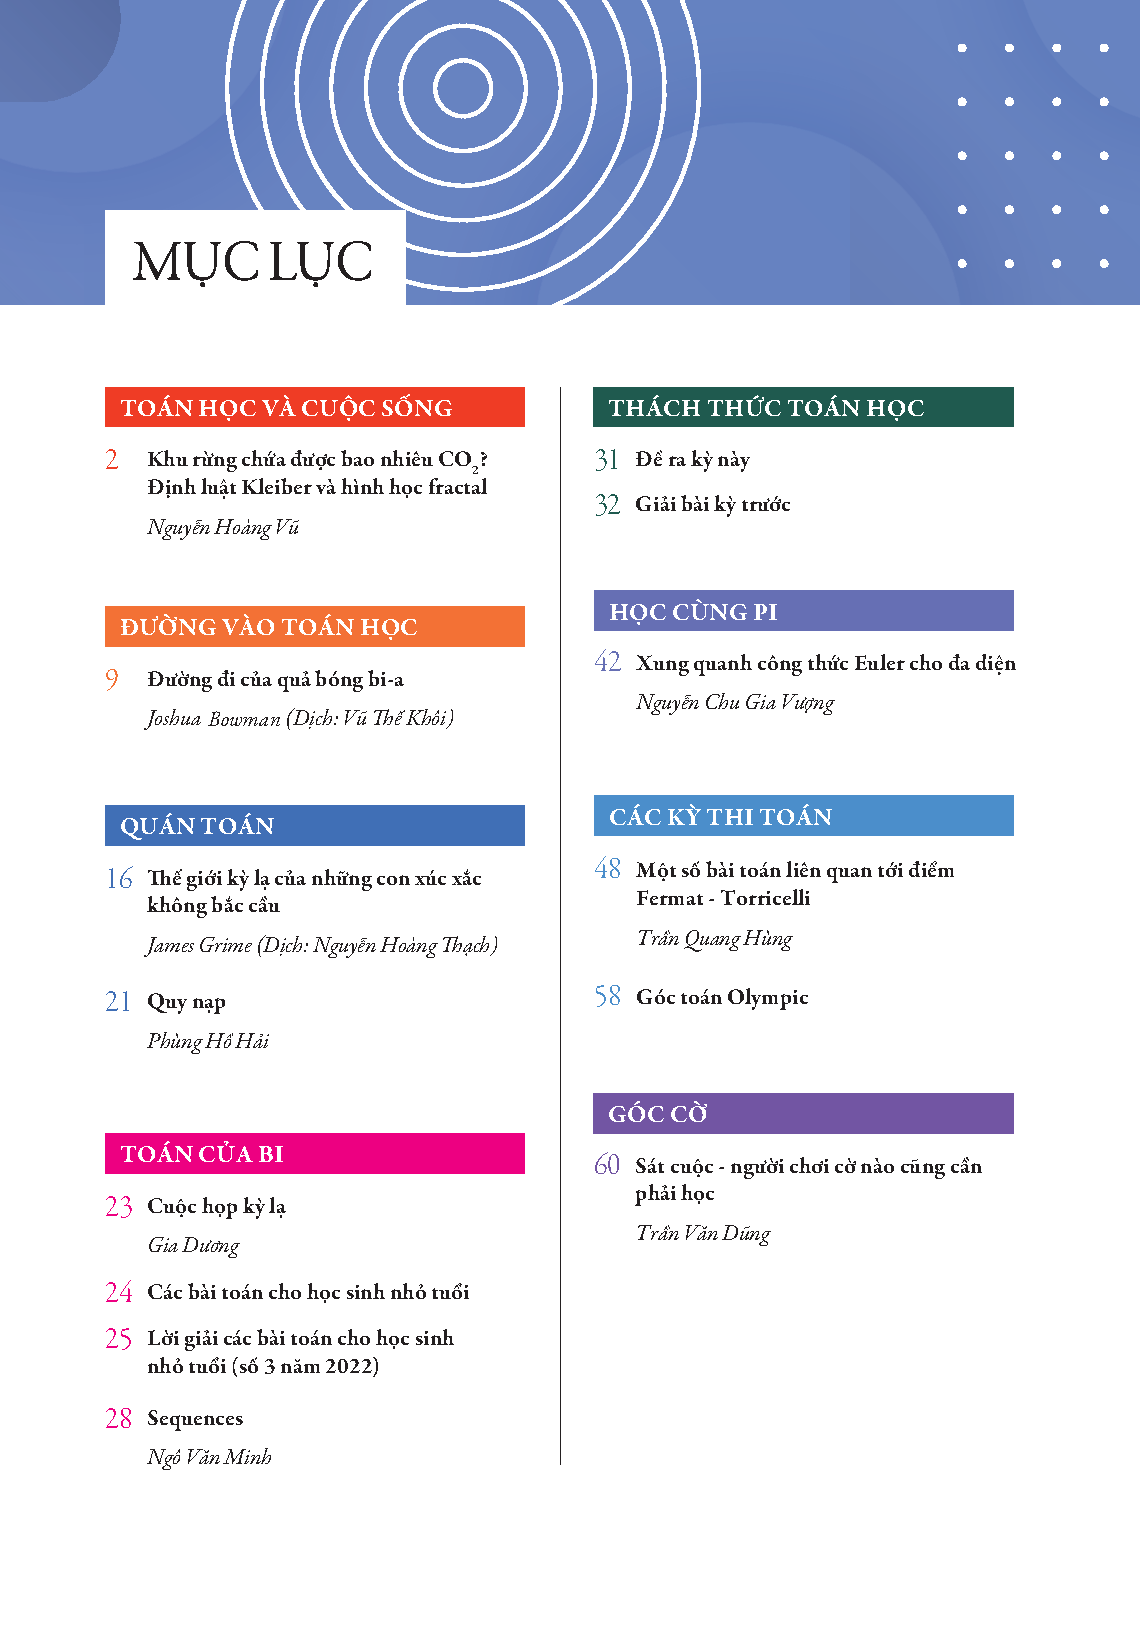
\includegraphics[scale=1]{ML.pdf}}}
%	 \centering
%	 \vspace*{0cm}
%	 \endgroup
%	 \newpage	 
%	 \pagestyle{empty}

%	\setcounter{page}{2}
%	\setcounter{figure}{0}
%	\thispagestyle{toanhocvadoisongnone}
\pagestyle{toanhocvadoisong}
\everymath{\color{toanhocdoisong}}
\graphicspath{{../toanhocdoisong/pic/}}
\begingroup
\blfootnote{$^1$\color{toanhocdoisong}Viện Sinh thái và Môi trường Đông Dương.}
\AddToShipoutPicture*{\put(0,616){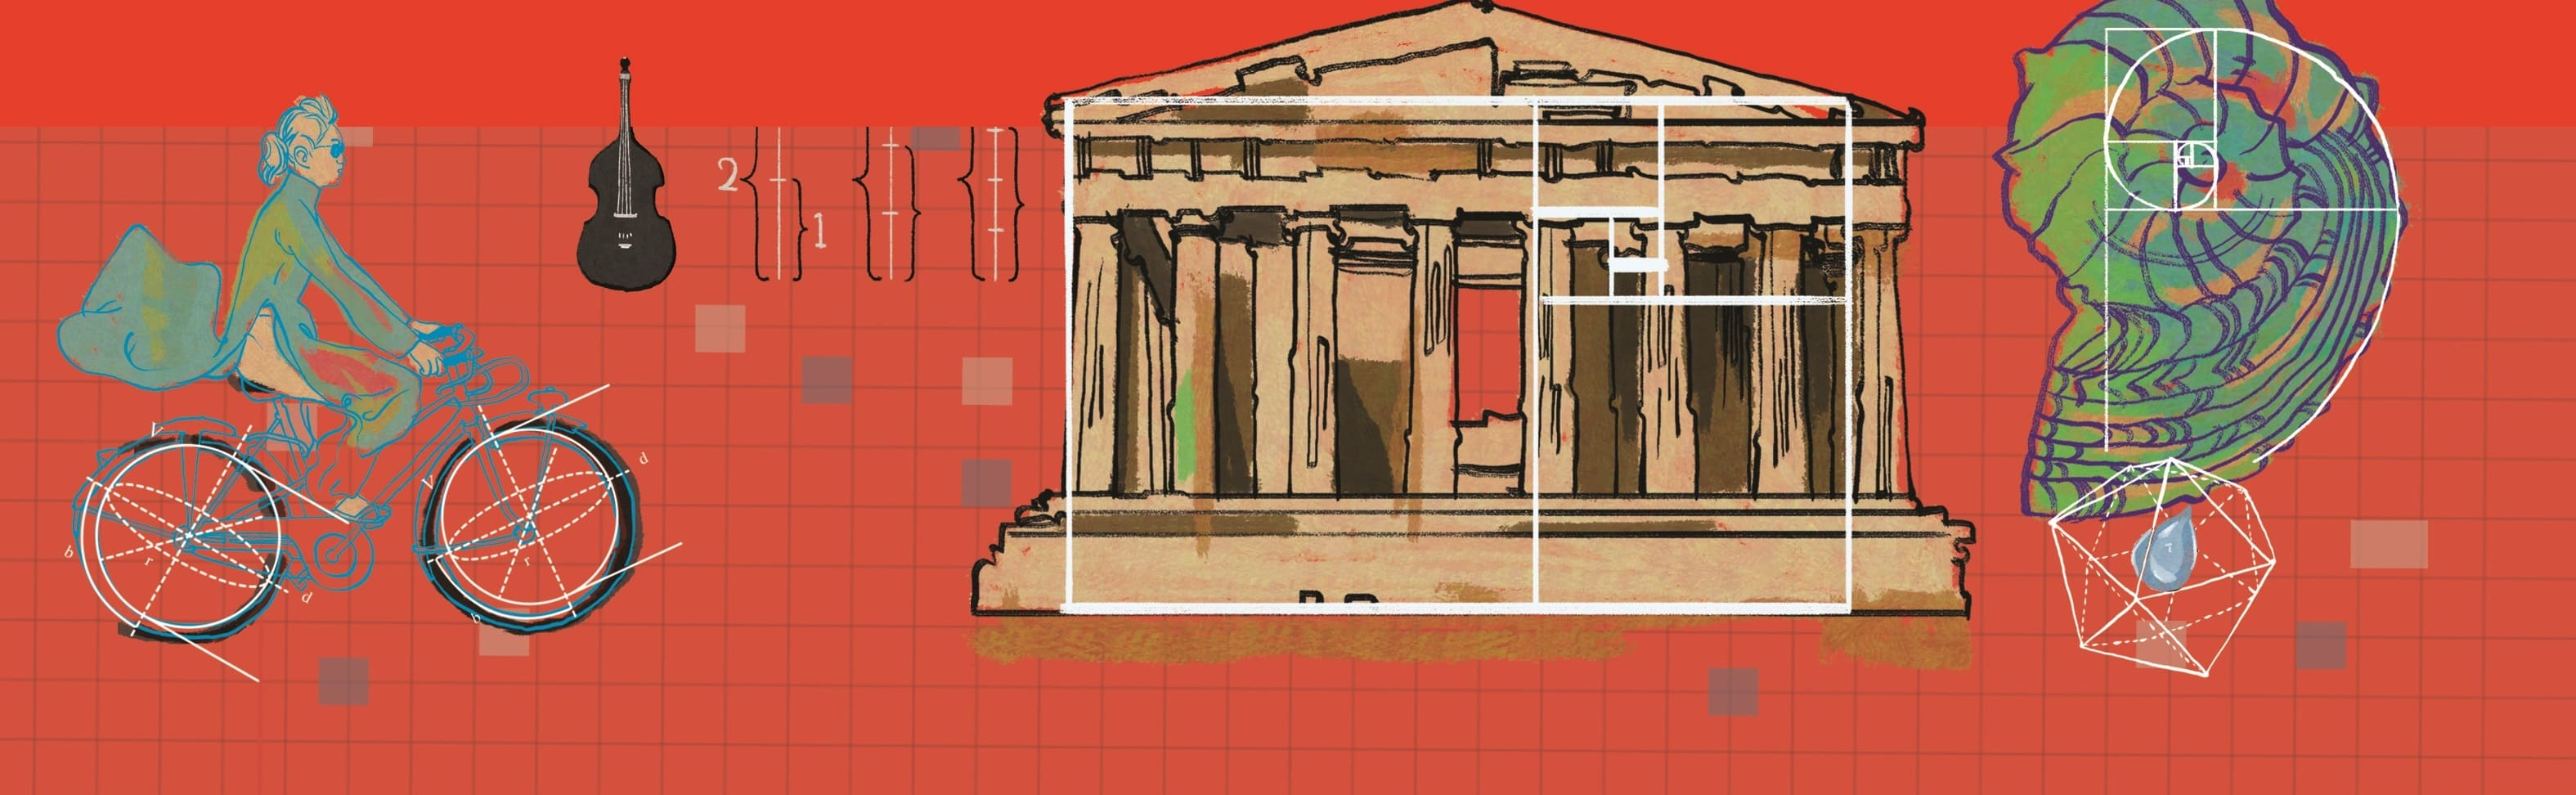
\includegraphics[width=19.3cm]{../bannertoanhocdoisong}}}
\AddToShipoutPicture*{\put(79,520){
\includegraphics[scale=1]{../tieude.pdf}}}
\centering
\endgroup

\vspace*{190pt}

\begin{multicols}{2}
	Bài toán cây kim của Buffon vẫn luôn xuất hiện trong sách giáo khoa toán dưới dạng một phương pháp để tính số $\pi$. Trong bài này, chúng ta hãy cũng Pi tìm hiểu chi tiết về bài toán này cũng như một số ứng dụng thú vị của nó trong thực tiễn.
	
	\vskip 0.1cm
	\textbf{\color{toanhocdoisong}$\pmb{1.}$ Bài toán cây kim của Buffon}
	\begin{figure}[H]
		\vspace*{-5pt}
		\centering
		\captionsetup{labelformat= empty, justification=centering}
		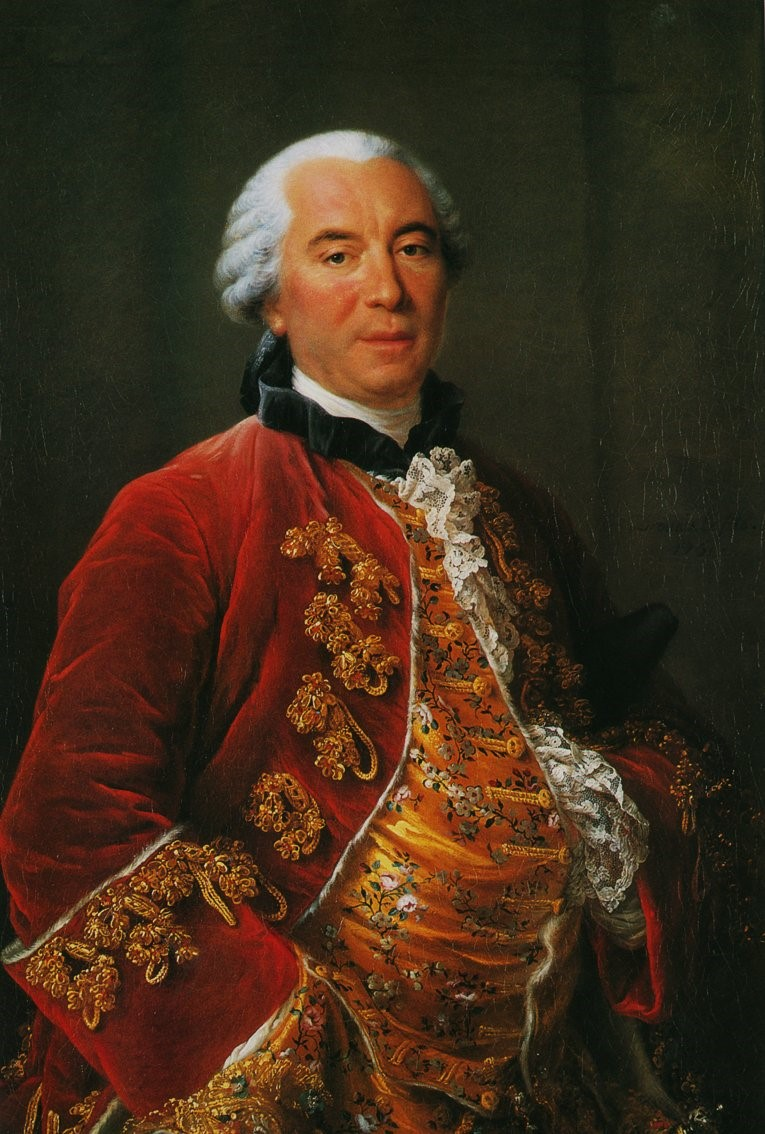
\includegraphics[width=0.6\linewidth]{1}
		\caption{\small\textit{\color{toanhocdoisong}Georges--Louis Leclerc, Comte de Buffon $(1707-1788)$.}}
		\vspace*{-10pt}
	\end{figure}
	Nhà toán học Pháp thế kỉ $18$, Georges Louis Leclerc, được phong Bá tước tại vùng có một ngôi làng tên Buffon nên ông còn có danh hiệu Comte de Buffon (Bá tước Buffon). Do đó các tài liệu thường gọi tắt là Buffon. Bài toán nổi tiếng mang tên ông có nội dung như sau:
	\vskip 0.1cm
	``Trên một tờ giấy với các đường kẻ cách đều nhau khoảng cách $d$, thả ngẫu nhiên một cây kim chiều dài $l$ $(d>l)$, hãy tìm xác suất để cây kim cắt một đường nằm ngang trên trang giấy".
	\begin{figure}[H]
		\vspace*{-5pt}
		\centering
		\captionsetup{labelformat= empty, justification=centering}
		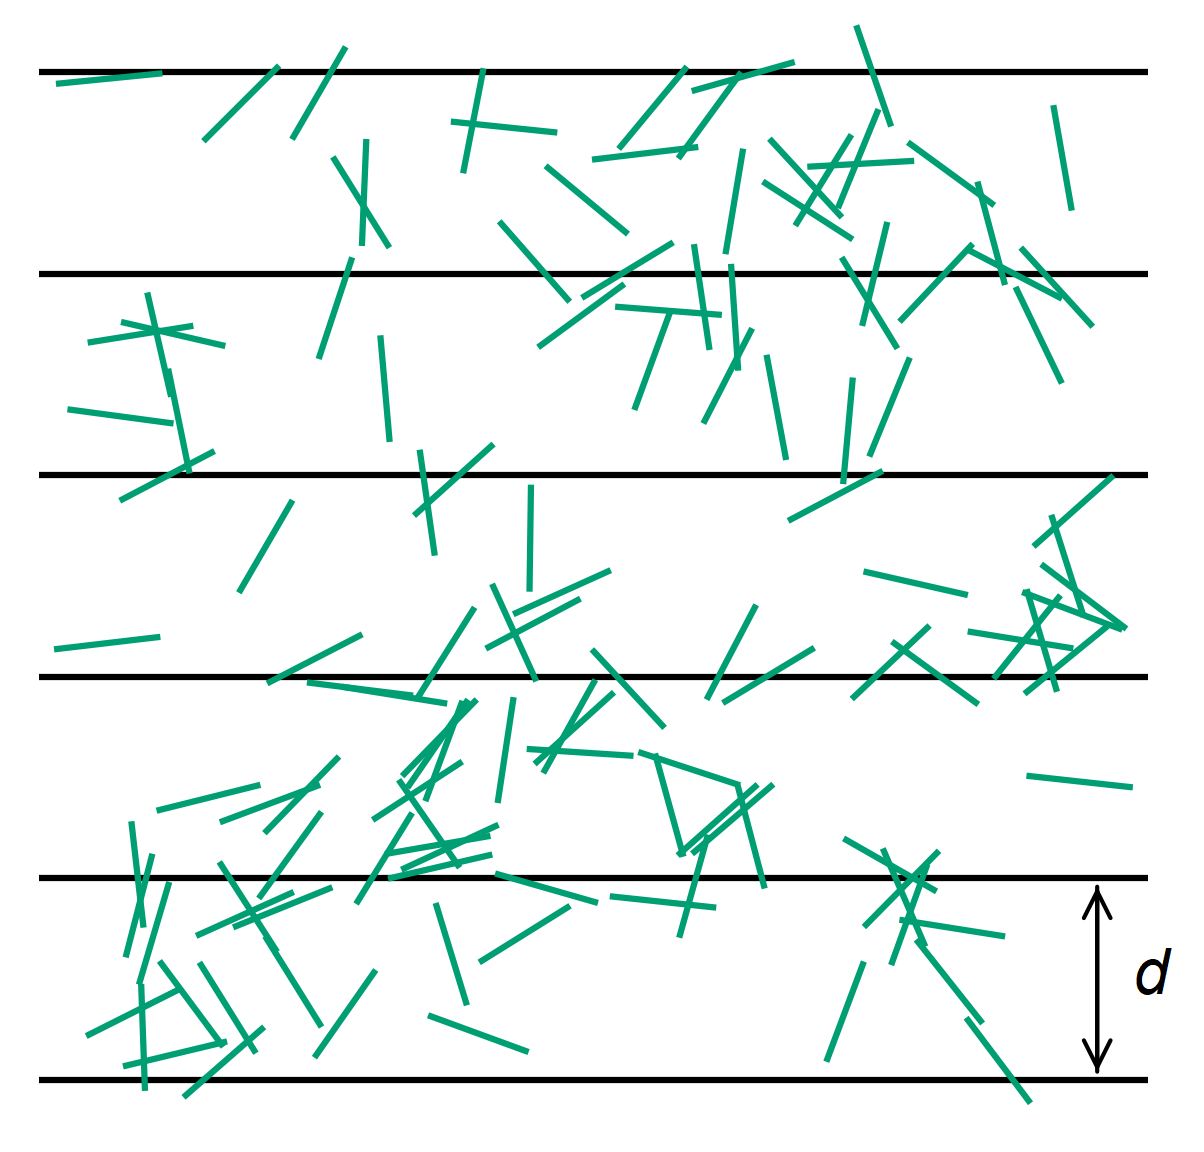
\includegraphics[width=0.95\linewidth]{2}
		\caption{\small\textit{\color{toanhocdoisong}Hình $1$. Minh họa bài toán cây kim của Buffon.}}
		\vspace*{-10pt}
	\end{figure}
	Chúng ta hãy xét một lời giải không sử dụng tích phân được E. Barbier đưa ra năm $1860$.
	\vskip 0.1cm 
	Do $l<d$ nên chỉ có hai trường hợp xảy ra: cây kim cắt một đường kẻ và cây kim không đè lên đường kẻ nào; không tồn tại trường hợp cây kim cắt nhiều hơn một đường kẻ.
	\vskip 0.1cm
	Gọi $P(l)$ là xác suất để cây kim có độ dài $l$ cắt một đường kẻ khi được thả. Lấy một điểm bất kỳ trên cây kim chia nó thành hai đoạn thẳng độ dài $l_1$ và $l_2$. Ta có:
	\begin{align*}
		P(l)=P(l_1 )+P(l_2).
	\end{align*}
	Quan hệ trên có thể được mở rộng ra thành dạng $P(l)=n\cdot P(\dfrac{l}{n})$. Tức là xác suất để một cây kim cắt đường kẻ khi được thả sẽ bằng $n$ lần xác suất này của cây kim có độ dài bằng $\dfrac{1}{n}$ lần độ dài cây kim ban đầu.
	\vskip 0.1cm
	Do đó, $P(l)=c\cdot l$ với $c$ là một hằng số, $c=P(1)$ (khi $l=1$ và $d > 1$).
	\begin{figure}[H]
		\vspace*{-5pt}
		\centering
		\captionsetup{labelformat= empty, justification=centering}
		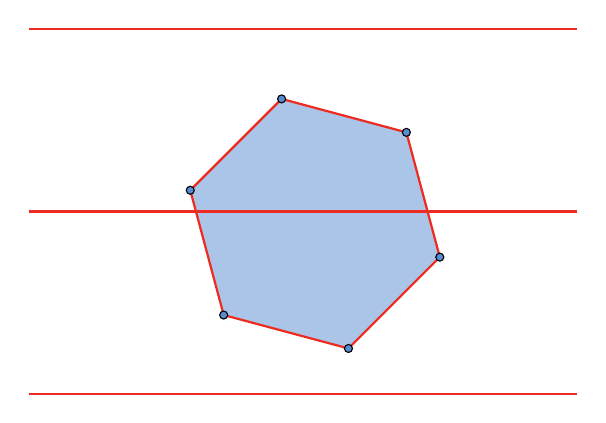
\begin{tikzpicture}[scale=0.58]
			\definecolor{qqqqff}{rgb}{0.,0.,1.}
			\definecolor{ududff}{rgb}{0.30196078431372547,0.30196078431372547,1.}
				\fill[line width=0.8pt,color=cackithi,fill=cackithi,fill opacity=0.5] (1.,3.) -- (3.,5.) -- (2.267949192431123,7.732050807568878) -- (-0.46410161513775494,8.464101615137755) -- (-2.4641016151377553,6.464101615137756) -- (-1.7320508075688794,3.7320508075688785) -- cycle;
				\draw [line width=0.8pt,color=toanhocdoisong] (1.,3.)-- (3.,5.);
				\draw [line width=0.8pt,color=toanhocdoisong] (3.,5.)-- (2.267949192431123,7.732050807568878);
				\draw [line width=0.8pt,color=toanhocdoisong] (2.267949192431123,7.732050807568878)-- (-0.46410161513775494,8.464101615137755);
				\draw [line width=0.8pt,color=toanhocdoisong] (-0.46410161513775494,8.464101615137755)-- (-2.4641016151377553,6.464101615137756);
				\draw [line width=0.8pt,color=toanhocdoisong] (-2.4641016151377553,6.464101615137756)-- (-1.7320508075688794,3.7320508075688785);
				\draw [line width=0.8pt,color=toanhocdoisong] (-1.7320508075688794,3.7320508075688785)-- (1.,3.);
				\draw [toanhocdoisong,line width=0.8pt] (-6.,6.)-- (6.,6.);
				\draw [toanhocdoisong,line width=0.8pt] (-6.,2.)-- (6.,2.);
				\draw [toanhocdoisong,line width=0.8pt] (-6.,10.)-- (6.,10.);
			
				\draw [fill=cackithi] (1.,3.) circle (2.5pt);
				\draw [fill=cackithi] (3.,5.) circle (2.5pt);
				\draw [fill=cackithi] (2.267949192431123,7.732050807568878) circle (2.5pt);
				\draw [fill=cackithi] (-0.46410161513775494,8.464101615137755) circle (2.5pt);
				\draw [fill=cackithi] (-2.4641016151377553,6.464101615137756) circle (2.5pt);
				\draw [fill=cackithi] (-1.7320508075688794,3.7320508075688785) circle (2.5pt);
		\end{tikzpicture}
		\caption{\small\textit{\color{toanhocdoisong}Hình $2$. Thả một đa giác cạnh $l$ lên tờ giấy với các đường kẻ ngang cách đều nhau.}}
		\vspace*{-10pt}
	\end{figure}
	Ta hãy tiếp tục xét một đa giác đều $N$ cạnh có độ dài mỗi cạnh bằng $l$ (Hình $2$). Ta đã biết ở trên rằng xác suất để mỗi cạnh của đa giác cắt một đường kẻ là $P(l)$. Đây cũng chính là giá trị kỳ vọng của số giao điểm của một cạnh với các đường kẻ, vì số giao điểm nói chung chỉ có thể là $0$ hoặc $1$ tương ứng với không cắt và cắt. Theo tính chất cộng tính của kỳ vọng, giá trị kỳ vọng của số giao điểm của đa giác với các đường kẻ khi thả lên tờ giấy là:
	\begin{align*}
		E &= \sum\nolimits_{i = 1}^N {P(l) = N \cdot } P(l) \\
		&= N \cdot c \cdot l = c \cdot L, \tag{$1$}
	\end{align*}
	với $L=N \cdot l$ là chu vi của đa giác đều.
	\vskip 0.1cm
	\columnbreak
	\textbf{\color{toanhocdoisong}Giá trị kỳ vọng}
	\vskip 0.1cm
	Trong một thí nghiệm ngẫu nhiên, nếu kết quả có giá trị $x_i$ có xác suất xảy ra là $p_i$ thì giá trị kỳ vọng của kết quả thu được được tính theo công thức:
	\begin{align*}
		E=x_1 p_1+x_2 p_2+ \cdots +x_n p_n.
	\end{align*}
	Ví dụ, với thí nghiệm gieo con xúc xắc, giá trị kỳ vọng của số chấm thu được là:
	\begin{align*}
		E=\frac{1}{6}\cdot 1 + \frac{1}{6} \cdot 2 + \cdots + \frac{1}{6}\cdot6 = 3{,5}.
	\end{align*}
	Chú ý rằng giá trị kỳ vọng có thể không trùng với một trong các giá trị có thể xảy ra. Theo định luật số lớn trong xác suất, với số lần thực hiện thí nghiệm càng lớn thì giá trị trung bình của các kết quả sẽ càng đến gần với giá trị kỳ vọng.
	\vskip 0.1cm
	Mặt khác, nếu giữ chu vi $L$ của đa giác không đổi, khi $N \to \infty$, đa giác của ta sẽ trở thành một đường tròn có chu vi $L$ và bán kính $\dfrac{L}{2\pi}$.
	\vskip 0.1cm
	Để tính hệ số $c$, ta xét một trường hợp đặc biệt, khi đường tròn có đường kính đúng bằng khoảng cách $d$ giữa các dòng kẻ. Khi đó, ta có $L=\pi d$.
	\begin{figure}[H]
		\vspace*{-5pt}
		\centering
		\captionsetup{labelformat= empty, justification=centering}
		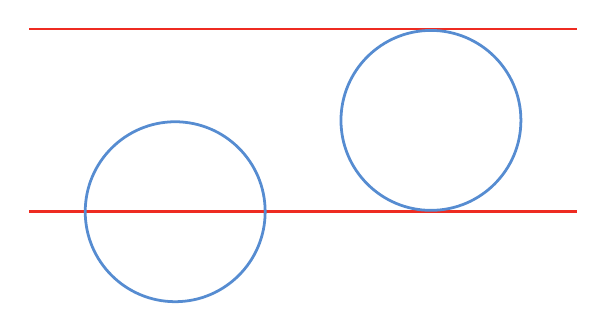
\begin{tikzpicture}[scale=0.58]
			\draw [toanhocdoisong, line width=1.pt] (-6.,6.)-- (6.,6.);
			\draw [toanhocdoisong, line width=1.pt] (-6.,10.)-- (6.,10.);
			\draw [cackithi, line width=1.pt] (2.8,8.) circle (1.97cm);
			\draw [cackithi, line width=1.pt] (-2.8,6.) circle (1.97cm);
		\end{tikzpicture}
		\caption{\small\textit{\color{toanhocdoisong}Hình $3$. Đường tròn có đường kính $d$ sẽ luôn cắt một đường kẻ tại hai điểm hoặc tiếp xúc hai đường kẻ.}}
		\vspace*{-10pt}
	\end{figure}
	Đường tròn có đường kính $d$ sẽ luôn cắt một đường kẻ tại $2$ giao điểm hoặc tiếp xúc với $2$ đường kẻ liên tiếp, do đó với đường tròn này $E=2$. Thay vào ($1$) ta có:
	\begin{align*}
		2=c\cdot\pi d
	\end{align*}
	hay $c = \dfrac{2}{\pi d}$.
	\vskip 0.1cm
	Vậy xác suất để một cây kim khi thả cắt đường nằm ngang trên giấy là 
	\begin{align*}
		P(l) = \frac{2l}{\pi d}. \tag{$2$}
	\end{align*}
	\begin{figure}[H]
		\vspace*{-5pt}
		\centering
		\captionsetup{labelformat= empty, justification=centering}
		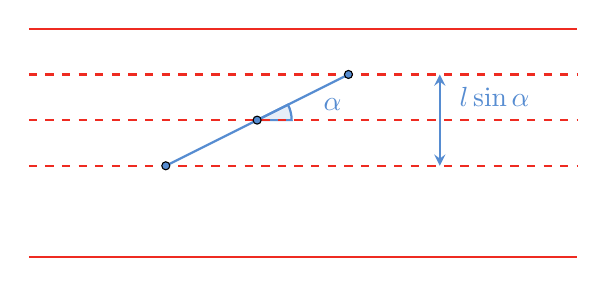
\begin{tikzpicture}[scale=0.58]
			\draw [shift={(-1.,8.)},line width=0.8pt,color=cackithi,fill=cackithi,fill opacity=0.15000000596046448] (0,0) -- (0.:0.7555063451882832) arc (0.:26.56505117707799:0.7555063451882832) -- cycle;
			\draw [toanhocdoisong,line width=0.8pt] (-6.,10.)-- (6.,10.);
			\draw [toanhocdoisong,dashed, line width=0.8pt] (-6.,9.)-- (6.,9.);
			\draw [toanhocdoisong,dashed, line width=0.8pt] (-6.,8.)-- (6.,8.);
			\draw [toanhocdoisong,dashed, line width=0.8pt] (-6.,7.)-- (6.,7.);
			\draw [toanhocdoisong, line width=0.8pt] (-6.,5.)-- (6.,5.);
			\draw [cackithi,line width=0.8pt] (-3.,7.)-- (1.,9.);
			\draw [fill=cackithi] (-3,7) circle (2.5pt);
			\draw [fill=cackithi] (1,9) circle (2.5pt);
			\draw [fill=cackithi] (-1,8) circle (2.5pt);
			\draw [cackithi,-stealth,line width=0.8pt] (3.,8.)-- (3.,9.);
			\draw [cackithi,-stealth,line width=0.8pt] (3.,8.)-- (3.,7.);
			
			\draw[color=cackithi] (0.65,8.347966297286694) node {$\color{cackithi}\alpha$};
			\draw[color=cackithi] (4.2,8.5) node {$\color{cackithi}l\sin\alpha$};
		\end{tikzpicture}
		\caption{\small\textit{\color{toanhocdoisong}Hình $4$. Chứng minh công thức $(2)$ sử dụng tích phân.}}
		\vspace*{-10pt}
	\end{figure}
	Ta cũng có thể thu được đáp án này bằng cách sử dụng tích phân. Cụ thể là ta xây dựng một mô hình xác suất cho vị trí rơi của cây kim. Gọi $\alpha$ $(0\le \alpha \le \dfrac{\pi}{2})$ là góc mà cây kim tạo với phương nằm ngang. Hình chiếu của nó theo phương vuông góc với các đường kẻ sẽ có độ dài $l\sin\alpha$, mà khoảng cách giữa hai đường kẻ là $d$, do đó xác suất để nó cắt một đường kẻ là $\dfrac{l\sin\alpha}{d}$. Coi phân bố của $\alpha$ là đều trên khoảng $[0,\dfrac{\pi}{2}]$, ta tính giá trị trung bình bằng cách lấy tích phân trên khoảng này rồi chia cho $\dfrac{\pi}{2}$ để thu được ($2$):
	\begin{align*}
		P(l) &= \frac{2}{\pi }\int_0^{\frac{\pi }{2}} {\frac{{l\sin \alpha }}{d}} d\alpha  = \frac{2}{\pi }\frac{l}{d}\left[ { - \cos \alpha } \right]|_0^{\frac{\pi }{2}}\\
		& = \frac{2}{\pi }\frac{l}{d}.
	\end{align*}
	Với cây kim có độ dài lớn hơn $d$, xác suất để nó cắt ít nhất một đường kẻ trong khoảng $\left[\arcsin\left(\dfrac{d}{l}, \dfrac{\pi}{2}\right)\right]$ sẽ luôn là $1$, do đó:
	\begin{align*}
		&P(l) \\
		= \,&\frac{2}{\pi }\left( {\int_0^{\arcsin \left( {\frac{d}{l}} \right)} {\frac{{l\sin \alpha }}{d} + } \int_{\arcsin \left( {\frac{d}{l}} \right)}^{\frac{\pi }{2}} {1d\alpha } } \right)\\
		=\,&1 \!\!+\!\! \frac{2}{\pi }\!\left( \!\!{\frac{l}{d}\!\!\left(\!\! {1 \!-\! \sqrt {\!\!1 \!-\! \frac{{{d^2}}}{{{l^2}}}} \!} \right) \!\!-\! \arcsin\! \frac{d}{l}}\! \right)\!\!.\tag{$3$}
	\end{align*}
	Bài toán này cũng được Laplace mở rộng cho trường hợp lưới trên tờ giấy là lưới chữ nhật và  tính xác suất để cây kim không cắt một đường kẻ dọc hay ngang nào. 
	\vskip 0.1cm
	Cũng chính Laplace đã đề xuất sử dụng thí nghiệm này để tính giá trị của số $\pi$. Đây cũng là khía cạnh được biết đến nhiều nhất về bài toán cây kim của Buffon. Thật vậy, nếu trong $M$ lần thả cây kim, ta thu được $m$ lần mà nó cắt một đường kẻ, công thức ($2$) cho ta:
	\begin{align*}
		\pi = \frac{2l}{d\cdot\left(\frac{m}{M}\right)},
	\end{align*}
	với $\dfrac{m}{M}$ là xác suất thực nghiệm của sự kiện cây kim cắt một đường kẻ.
	\vskip 0.1cm
	Đề xuất này của Laplace rất gần với phương pháp Monte Carlo của hơn một thế kỉ sau. Tuy vậy, về mặt thực tế, nó gập phải một số vấn đề. Nhiều thí nghiệm được tiến hành và cho kết quả của $\pi$ không quá chính xác: $3{,}1596$; $3{,}1553$; $3{,}137$.
	\vskip 0.1cm 
	Năm $1901$, Lazzarini công bố giá trị $3{,}1415929$ cho $3408$ lần thả cây kim, một giá trị khá chính xác (so với giá trị đã biết hiện nay, thì chỉ có chữ số cuối là không đúng). Tuy vậy, một số nghiên cứu đã chỉ ra kết quả này hầu như là ngụy tạo. Theo các lí thuyết về ước lượng tham số, để có độ chính xác đến $6$ chữ số sau dấu phẩy, cần phải tiến hành thí nghiệm trên $1{,}34×10^{14}$ lần chứ không phải vài nghìn lần. Đồng thời, số liệu của Lazzarini sử dụng phân số $\dfrac{355}{113}$, một số hữu tỉ được biết là một xấp xỉ tốt cho $\pi$. 
	\vskip 0.1cm
	Ngay cả với máy tính điện tử thì việc ước lượng $\pi$ bằng cách sử dụng thí nghiệm Buffon cũng không đạt được độ chính xác quá cao do việc làm tròn số trên máy tính. Đồng thời, các chữ số của $\pi$ cũng có thể được tính toán một cách chính xác hơn bởi các phương pháp khác.
	\vskip 0.1cm
	Tuy vậy, bài toán cây kim của Buffon có một ý nghĩa quan trọng trong lịch sử toán học bởi sự liên hệ giữa xác suất và hình học. Đây là một hướng tiếp cận mới khác với hướng tiếp cận xác suất sử dụng tổ hợp như truyền thống.
	\vskip 0.1cm
	\textbf{\color{toanhocdoisong}Bài tập}
	\vskip 0.1cm
	$1$. Chứng minh rằng khi cây kim vô cùng dài thì một cách hầu chắc chắn nó sẽ luôn cắt ít nhất một đường kẻ, tức là biểu thức trong ($3$) có giới hạn là $1$ khi $l\to \infty$.
	\vskip 0.1cm
	$2$. Trên tờ giấy với các đường kẻ ngang cách nhau khoảng $d$, thả ngẫu nhiên một đường tròn với bán kính $r < \dfrac{d}{2}$. Hãy tính xác suất để đường tròn cắt và không cắt các đường kẻ.
	\vskip 0.1cm
	$3$. Tương tự bài trên nhưng thả một hình vuông có cạnh $a<d$. Hãy tính xác suất để số giao điểm của các cạnh hình vuông với các đường kẻ ngang là:
	\vskip 0.1cm
	$a)$ $0$\quad\quad		$b)$ $1$\quad\quad		$c)$ $2$\quad\quad
	$d)$ $3$\quad\quad		$e)$ $4$
	\vskip 0.1cm
	Gợi ý: Xét trường hợp $a<\dfrac{d}{\sqrt{2}}$ và $a> \dfrac{d}{\sqrt{2}}$.
	\vskip 0.1cm	
	$4$. Trong thí nghiệm Buffon, với cây kim có độ dài $l>d$, hãy chứng minh giá trị kỳ vọng của số giao điểm của cây kim với các đường kẻ ngang là $E = \dfrac{2l}{\pi d}$. (Gợi ý: Gọi $N$ là số nguyên lớn nhất sao cho $d<\dfrac{l}{N}$, coi cây kim là hình gồm $N$ đoạn thẳng bằng nhau).
	\vskip 0.1cm
	$5$. Mở rộng của Laplace. Trên một lưới chữ nhật, với mỗi hình chữ nhật có chiều dài $a$ và chiều rộng $b$, thả ngẫu nhiên một cây kim chiều dài $l$ (biết rằng $l$ nhỏ hơn cả $a$ và $b$). Hãy tính xác suất để cây kim không chạm bất kỳ cạnh nào của lưới.
	\vskip 0.1cm
	$6$. Lưới Uspensky. Cho một lưới tam giác đều như hình vẽ với $d$ là chiều cao của mỗi tam giác đều. Thả một cây kim chiều dài \linebreak$l<d$ lên lưới tam giác đều này. Hãy tính xác suất để số giao điểm của cây kim với các đường trong lưới là:
	\vskip 0.1cm
	\quad\quad$a)$ $0$\quad\quad		$b)$ $1$\quad\quad		$c)$ $2$	\quad\quad	$d)$ $3$
	\begin{figure}[H]
		\vspace*{5pt}
		\centering
		\captionsetup{labelformat= empty, justification=centering}
		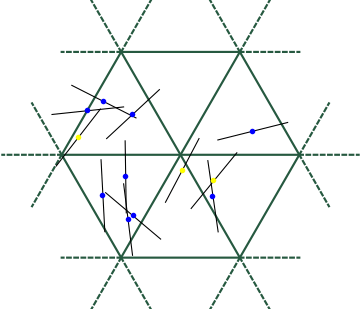
\includegraphics[width=1\linewidth]{6}
		\vspace*{-15pt}
	\end{figure}
	$7$. Bài toán sợi mì của Buffon. Trên một tờ giấy với các đường kẻ ngang song song cách nhau khoảng $d$, ném ngẫu nhiên một sợi mì ướt có độ dài $l$. Chứng minh rằng giá trị kì vọng của số giao điểm của sợi mì với các đường kẻ ngang là $E=\dfrac{2l}{\pi d}$. Giả sử rằng khi ném sợi mì, chiều dài của nó không đổi nhưng nó có thể uốn thành một đường cong bất kỳ.
	\vskip 0.1cm
	\textbf{\color{toanhocdoisong}$\pmb{2.}$ Đo độ dài bằng phương pháp ngẫu nhiên}
	\vskip 0.1cm
	Với một số thay đổi, thí nghiệm của Buffon có thể được sử dụng để giải quyết một vấn đề thực tế trong khoa học: đo độ dài của rễ cây (Newman, $1966$). Xét một bản thủy tinh mà trên đó một mẫu vật (ví dụ rễ cây) được trải phẳng. Khi quan sát mẫu vật qua kính hiển vi, người ta sử dụng một thị kính với một đường sợi tóc để soi các vùng khác nhau của bản thủy tinh.
	\vskip 0.1cm
	Với mỗi lần quan sát, thị kính được quay một góc bất kì và đường sợi tóc cũng được quay theo. Sau đó, số giao điểm của đường sợi tóc với rễ cây sẽ được ghi lại. Cách thức này được lặp lại nhiều lần với các vị trí quan sát ngẫu nhiên khác nhau trên bản thủy tinh. Để tiện lợi hơn, ta có thể đặt bản thủy tinh trên một tấm giấy với các điểm ngẫu nhiên đã được đánh dấu trước. Các điểm quan sát cũng có thể là một lưới ô vuông các điểm cách đều.
	\begin{figure}[H]
%		\vspace*{5pt}
		\centering
		\captionsetup{labelformat= empty, justification=centering}
		
\includegraphics[width=1\linewidth]{7}
		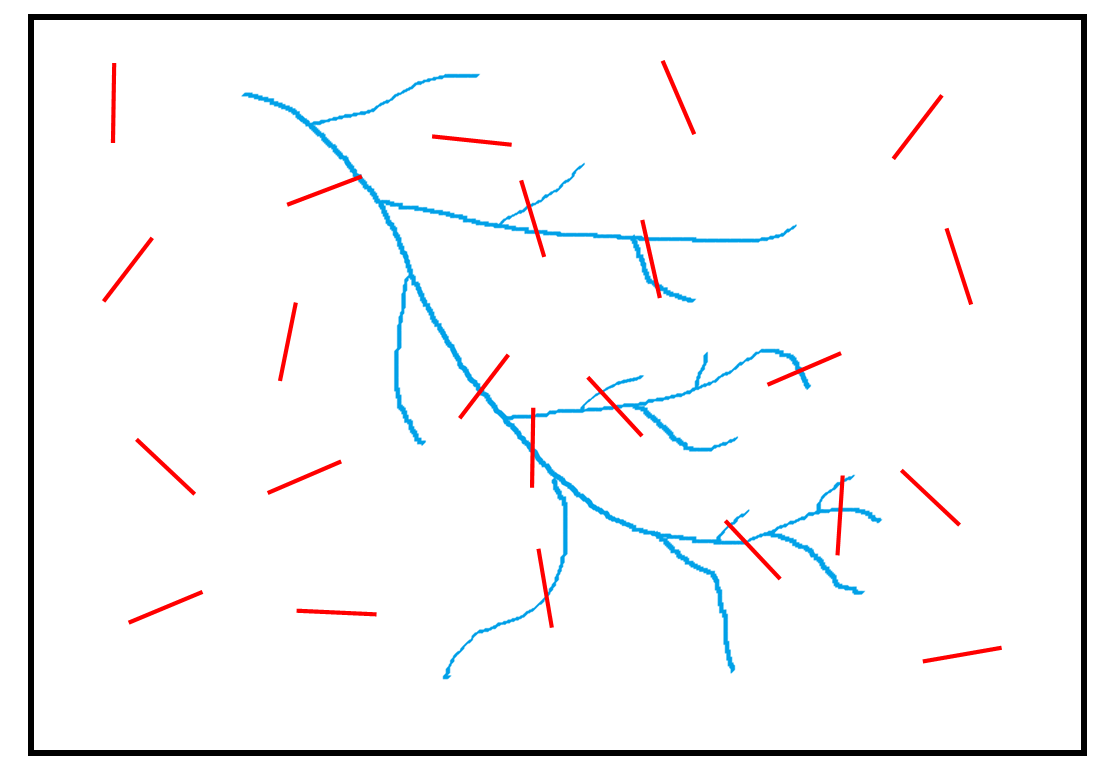
\includegraphics[width=1\linewidth]{8}
		\caption{\small\textit{\color{toanhocdoisong}Hình $5$. Trên: Thị kính của kính hiển vi có đường sợi tóc (đường thẳng đứng). Dưới: minh họa phép đo độ dài rễ cây (màu xanh) với các vị trí và góc quay khác nhau của đường sợi tóc (màu đỏ). Số lượng đường sợi tóc trong hình chỉ mang tính minh họa, trong thực tế, cấu trúc rễ cây càng phức tạp thì số lượng đường sợi tóc cần sử dụng lại càng nhiều. Mỗi lần quan sát qua kính, ta chỉ thấy được một vùng hình tròn có đường kính là đường sợi tóc.}}
		\vspace*{-10pt}
	\end{figure}
	Về mặt bản chất, thay vì đếm số giao điểm của cây kim được thả ngẫu nhiên với các đường kẻ ngang, ta đếm số giao điểm của các đường sợi tóc được phân bố ngẫu nhiên với mẫu vật rễ cây (gồm nhiều đường cong) trên bản thủy tinh.
	\vskip 0.1cm
	Độ dài của rễ cây có thể được tính theo công thức:
	\begin{align*}
		R= \frac{\pi N A}{2H},	\tag{$4$}
	\end{align*}
	với $N$ là số giao điểm đã được đếm, $A$ là diện tích bản thủy tinh và $H$ là tổng độ dài của tất cả các đường sợi tóc.
	\vskip 0.1cm
	Thật vậy, xét một đoạn rễ cây $PQ$ có chiều dài $\Delta R$ và một đường sợi tóc $MN$ chiều dài $h$. Nếu khoảng cách từ trung điểm $D$ của $PQ$ đến $MN$ lớn hơn $\dfrac{1}{2}\Delta R$ thì $PQ$ và $MN$ chắc chắn không cắt nhau. Miền giới hạn này được biểu diễn bằng đường nét đứt trong hình. Giả sử $\dfrac{\Delta R}{h}$ là nhỏ, diện tích miền này có thể được xấp xỉ bằng $\Delta \cdot h$. Do $MN$ được phân bố ngẫu nhiên trên bản thủy tinh, xác suất để $D$ nằm trong miền này là $\dfrac{\Delta R \cdot h}{A}$.
	\vskip 0.1cm
	Khi $D$ nằm trong miền cách $MN$ một khoảng không quá $\dfrac{1}{2}\Delta R$, khoảng cách từ $D$ đến $MN$ cần phải không lớn hơn $\dfrac{1}{2}\Delta R |\sin \theta |$, với $\theta$ là góc tạo bởi hai đường thẳng $PQ$ và $MN$, để $PQ$ và $MN$ cắt nhau. Xác suất để $PQ$ và $MN$ cắt nhau khi $D$ đã nằm trong miền trên là:
	\begin{align*}
		\frac{\frac{1}{2}\Delta R|\sin\theta|}{\frac{1}{2}\Delta R} = |\sin\theta|.
	\end{align*}
	Do đó, theo công thức nhân xác suất, xác suất để $PQ$ và $MN$ cắt nhau là:
	\begin{align*}
		p = \frac{\Delta R\cdot h}{A} |\sin\theta|.
	\end{align*}
	\begin{figure}[H]
		\vspace*{-5pt}
		\centering
		\captionsetup{labelformat= empty, justification=centering}
		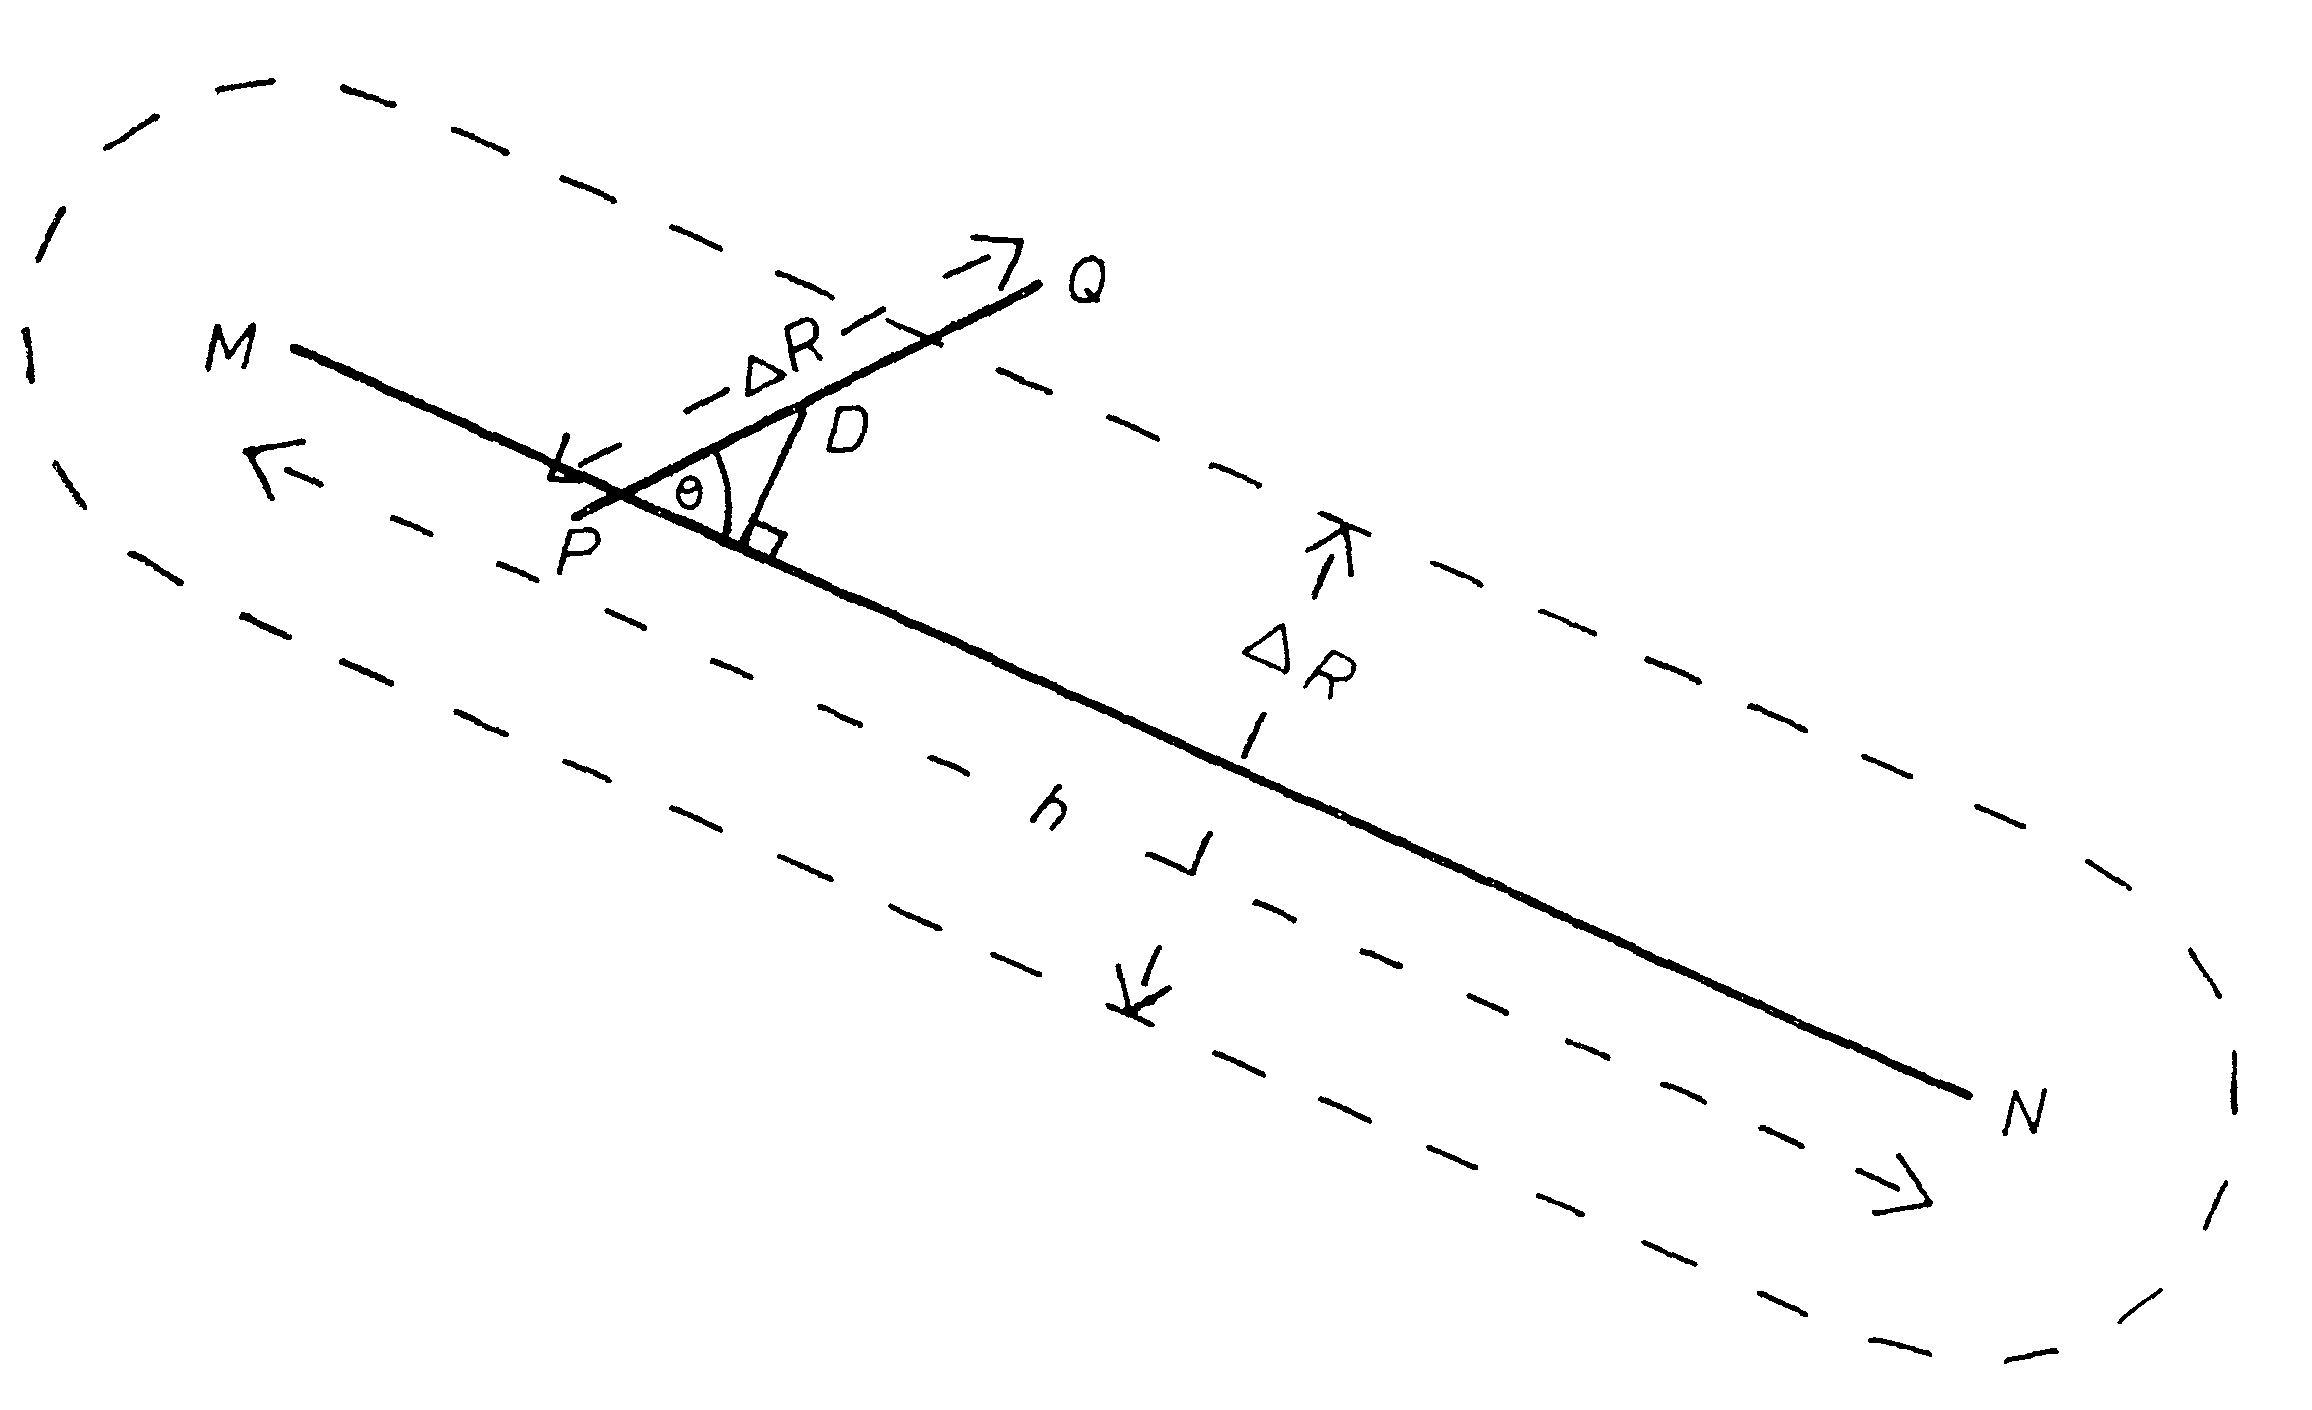
\includegraphics[width=1\linewidth]{9}
		\caption{\small\textit{\color{toanhocdoisong}Hình $6$. Đoạn rễ cây $PQ$ và đường sợi tóc $MN$.}}
		\vspace*{-10pt}
	\end{figure}
	Tổng độ dài của các đoạn sợi tóc được phân bố ngẫu nhiên trên miền diện tích $A$ là $H$. Các góc $\theta$ cũng nhận giá trị ngẫu nhiên trong khoảng $[0,2\pi]$ nên giá trị kì vọng của số giao điểm của $PQ$ với các đường sợi tóc là:
	\begin{align*}
		\frac{1}{2\pi}\int_0^{2\pi}{\frac{{\Delta R \cdot H}}{A}}|\sin\theta|d\theta= \frac{2\left(\Delta R \cdot H\right)}{\pi A}.
	\end{align*}
	Coi rễ cây là một hình với nhiều đoạn có độ dài $\Delta R$, ta được giá trị kì vọng của số giao điểm của rễ cây với tất cả các đường sợi tóc là:
	\begin{align*}
		N = \frac{2RH}{\pi A}.
	\end{align*}
	Do $N$ là giá trị kỳ vọng nên khi đo đạc người ta cần phải tiến hành nhiều lần quan sát với các vị trí ngẫu nhiên của đường sợi tóc để kết quả thí nghiệm gần với giá trị của $N$ trong công thức.
	\vskip 0.1cm
	Ví dụ, với bản thủy tinh $10\times 20$ cm; tiến hành quan sát $40$ lần, độ dài đường sợi tóc (đường kính của thị trường vùng quan sát được) là $1{,}88$ cm; số giao điểm quan sát được là $344$ thì tổng độ dài của rễ cây là:
	\begin{align*}
		R - \frac{\pi \cdot 344\cdot 10 \cdot 20}{2\cdot40 \cdot1{,}88} = 1436 \text{ cm}.
	\end{align*}
	Cách đo độ dài này đã được các nhà thực vật học sử dụng trong nhiều thập kỉ mãi cho đến gần đây mới được thay thế bởi các phần mềm xử lí ảnh từ các camera có độ phân giải cao.
	\vskip 0.1cm
	\textbf{\color{toanhocdoisong}$\pmb{3.}$ Kiến biết đo diện tích bằng xác suất?}
	\vskip 0.1cm
	Phương pháp đo độ dài ở phần trước cũng có thể được biến đổi để tiến hành đo diện tích.
	\vskip 0.1cm
	Một nghiên cứu khá thú vị trên loài kiến \textit{Leptothorax albipennis} đưa ra giả thuyết rằng loài kiến này đã sử dụng xác suất để tính diện tích khi chọn tổ (kiến thường cố gắng chọn tổ có diện tích lớn nhất trong các vị trí khảo sát) (Mallon \& Franks, $2000$).
	\vskip 0.1cm
	Khi sử dụng camera để theo dõi kiến trinh sát trong phòng thí nghiệm, người ta thấy trong lần thứ nhất đến một vị trí để khảo sát, con kiến sẽ đi một cách ngẫu nhiên trong hộp theo một đường cong bao phủ phần lớn các vị trí trong hộp (gọi là đường cong $L$). Trong những lần tiếp theo (thường nó sẽ quay lại lần thứ hai hoặc có thể là lần thứ $3$), nó sẽ đi một đường cong đơn giản hơn (gọi là đường cong $S$). Đồng thời, khi đến các vị trí đã đi qua (kiến khi di chuyển có thể tiết ra pheromone để đánh dấu đường đi của mình), tức là các giao điểm của $L$ và $S$, kiến dành thời gian lâu hơn nhiều.
	\begin{figure}[H]
		\vspace*{-5pt}
		\centering
		\captionsetup{labelformat= empty, justification=centering}
		
\includegraphics[width=0.65\linewidth]{10}
		\caption{\small\textit{\color{toanhocdoisong}Hình $7$. Từ trên xuống: Đường đi của kiến trinh sát khi khảo sát tổ được camera ghi lại trong lần khảo sát thứ nhất, thứ hai và thứ ba.}}
		\vspace*{-10pt}
	\end{figure}
	Theo các tác giả, số giao điểm của $L$ và $S$ được kiến trinh sát sử dụng để đánh giá diện tích của một vị trí làm tổ. Trong công thức ($4$), nếu ta thay các đường sợi tóc bằng một đường cong $L$ và rễ cây $R$ bằng đường cong $S$, công thức này vẫn đúng và diện tích có thể được xấp xỉ theo 
	\begin{align*}
		A = \frac{2SL}{\pi N}, \tag{$5$}
	\end{align*}
	với $N$ là số giao điểm của $S$ và $L$.
	\vskip 0.1cm
	Để kiểm chứng việc này, thí nghiệm được tiến hành với nhiều con kiến trinh sát khác nhau trên các loại hộp để làm tổ như trong hình vẽ.
	\vskip 0.1cm
	Trong thí nghiệm để chọn giữa hai tổ cùng chu vi (hình $8a$ và hình $8c$), kiến luôn chọn tổ có diện tích lớn hơn sau khi khảo sát cả hai. Do đó, diện tích chứ không phải chu vi mới là tiêu chí chọn tổ. Vì các tổ có một tấm chắn ở giữa (hình $8d$) cũng được chọn với khả năng tương tự như tổ bình thường, cho thấy số lần va chạm với chướng ngại vật trong tổ cũng không phải nhân tố quyết định.
	\begin{figure}[H]
		\vspace*{-5pt}
		\centering
		\captionsetup{labelformat= empty, justification=centering}
		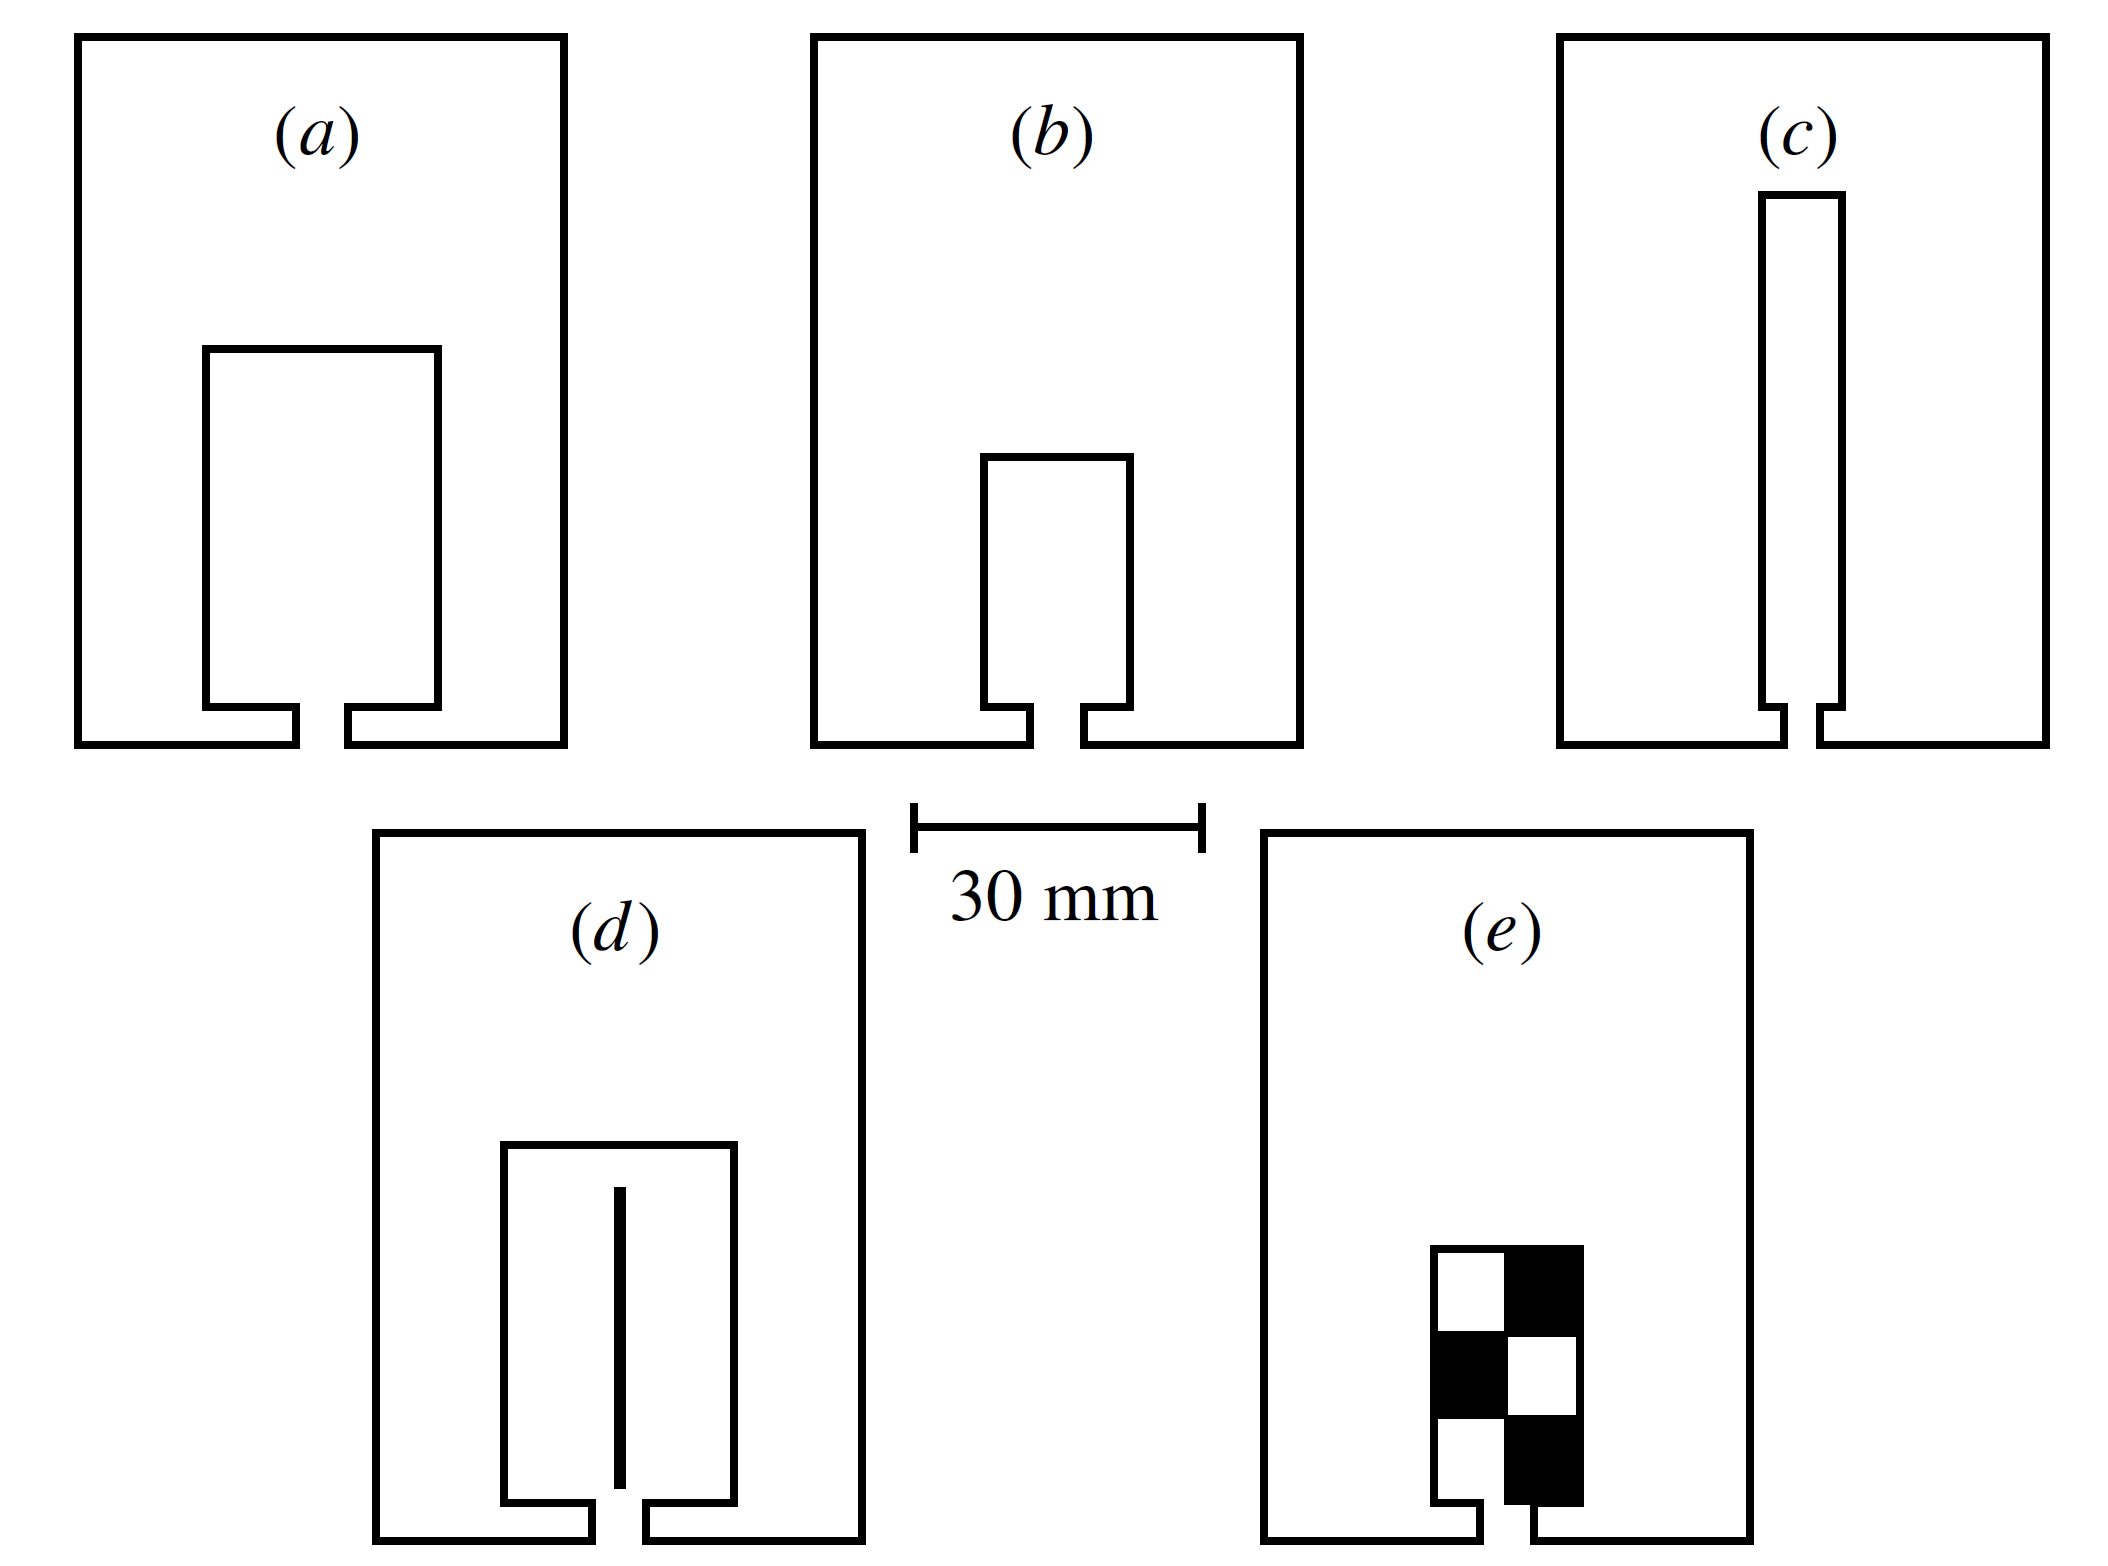
\includegraphics[width=1\linewidth]{11}
		\caption{\small\textit{\color{toanhocdoisong}Hình $8$. Các loại tổ được sử dụng trong thí nghiệm về việc chọn tổ của kiến trinh sát. $a)$ tổ tiêu chuẩn; $b)$ tổ đồng dạng và có diện tích bằng một nửa tổ tiêu chuẩn; $c)$ tổ có diện tích bằng một nửa tổ tiêu chuẩn nhưng có cùng chu vi; $d)$ tổ tiêu chuẩn có tấm chắn ở giữa; $e)$ tổ dạng $b$ với một nửa được phủ các tấm đệm có thể nhấc ra.}}
		\vspace*{-10pt}
	\end{figure}
	Thí nghiệm cũng cho thấy khi kiến trở lại lần thứ hai, nếu tổ đã được thay bằng một tổ mới hoặc một tổ đã được một con kiến khác đi qua, nó sẽ tiến hành khảo sát lại như là đang đi qua lần thứ nhất. Điều này cho thấy trong lần khảo sát thứ nhất, kiến sẽ lưu lại pheromone đánh dấu đường đi và pheromone này đặc trưng cho từng cá thể. Việc này cũng cho phép các con kiến không làm ảnh hưởng đến quá trình khảo sát của nhau khi một vị trí có thể được nhiều hơn một con kiến đến thăm dò.
	\vskip 0.1cm
	Nếu kiến trở lại lần thứ ba hoặc sau đó, thời gian nó tiến hành khảo sát cũng không khác nhiều lắm so với lần thứ hai, do đó có thể thấy pheromone chỉ được rải ở lần thăm dò thứ nhất còn các lần lặp lại sau để tăng độ chính xác của việc ước lượng.
	\vskip 0.1cm
	Loại tổ trong hình $8e$ được thiết kế đồng dạng với tổ trong hình $8a$ nhưng có diện tích bằng một nửa. Đồng thời, ở nền của loại tổ này, một nửa diện tích là các tấm đệm có thể lấy ra. Sau khi kiến khảo sát tổ dạng này lần thứ nhất, người ta sẽ lấy các tấm đệm ra trước khi kiến quay lại lần thứ hai. Khi kiến trở lại, do các vị trí có đệm bị lấy ra không còn pheromone nên số giao điểm của đường đi của nó trong lần thứ hai với đường đi trong lần thứ nhất sẽ giảm một nửa. Trong thí nghiệm chọn giữa tổ dạng $8a$ và dạng $8e$, một nửa số kiến chọn $8e$ dù diện tích chỉ có một nửa. Thí nghiệm với kích thước tổ lớn gấp đôi cho thấy khoảng cách $L$ của mỗi con kiến là không đổi giữa các tổ với diện tích khác nhau. Kết hợp với với ($5$), có thể thấy thấy kiến đánh giá diện tích theo tỉ lệ nghịch với tần số gặp giao điểm $\dfrac{N}{S}$.
	\vskip 0.1cm
	Việc nghiên cứu những thuật toán liên quan đến hành vi của kiến không chỉ có ý nghĩa về mặt sinh học mà còn có nhiều ứng dụng khác, ví dụ như trong việc lập trình điều khiển hành vi của robot.
	\vskip 0.1cm
	$\pmb{4.}$ \textbf{\color{toanhocdoisong}Lời kết}
	\vskip 0.1cm
	Lĩnh vực xác suất hình học còn có nhiều bài toán khác có giá trị về cả mặt lý thuyết lẫn thực tiễn. Pi cũng sẽ tiếp tục giới thiệu các bài toán này đến với độc giả trong tương lai không xa.
	\vskip 0.1cm
	\textbf{\color{toanhocdoisong}Tài liệu tham khảo}
	\vskip 0.1cm
	[$1$] Aigner, M., \& Ziegler, G. ($2004$). \textit{Proof from} THE BOOK. Springer--Verlag.
	\vskip 0.1cm
	[$2$] Mallon, E. B., \& Franks, N. R. ($2000$). Ants estimate area using Buffon's needle. \textit{Proc. R. Soc. Lond.} B($267$), $765-770$.
	\vskip 0.1cm
	[$3$] Mugford, S. T., Mallon, E. B., \& Franks, N. R. ($2001$). The accuracy of Buffon's needle: a rule of thumb used by ants to estimate area. \textit{Behavioral Ecology}, $12(6)$, $655-658$.
	\vskip 0.1cm
	[$4$] Newman, E. I. ($1966$). A Method of Estimating the Total Length of Root in a Sample. \textit{Journal of Applied Ecology}, $139-145$.
	\vskip 0.1cm
	[$5$] Ramaley, J. F. ($1969$). Buffon's Noodle Problem. \textit{The American Mathematical Monthly}, $78(8)$, $916-918$.
\end{multicols}
%	\newpage
	
%	\setcounter{figure}{0}
%	\thispagestyle{duongvaotoanhocnone}
\pagestyle{duongvaotoanhoc}
\everymath{\color{duongvaotoanhoc}}
\graphicspath{{../duongvaotoanhoc/pic/}}
%\blfootnote{$^1$\text{.}}
\begingroup
\AddToShipoutPicture*{\put(0,616){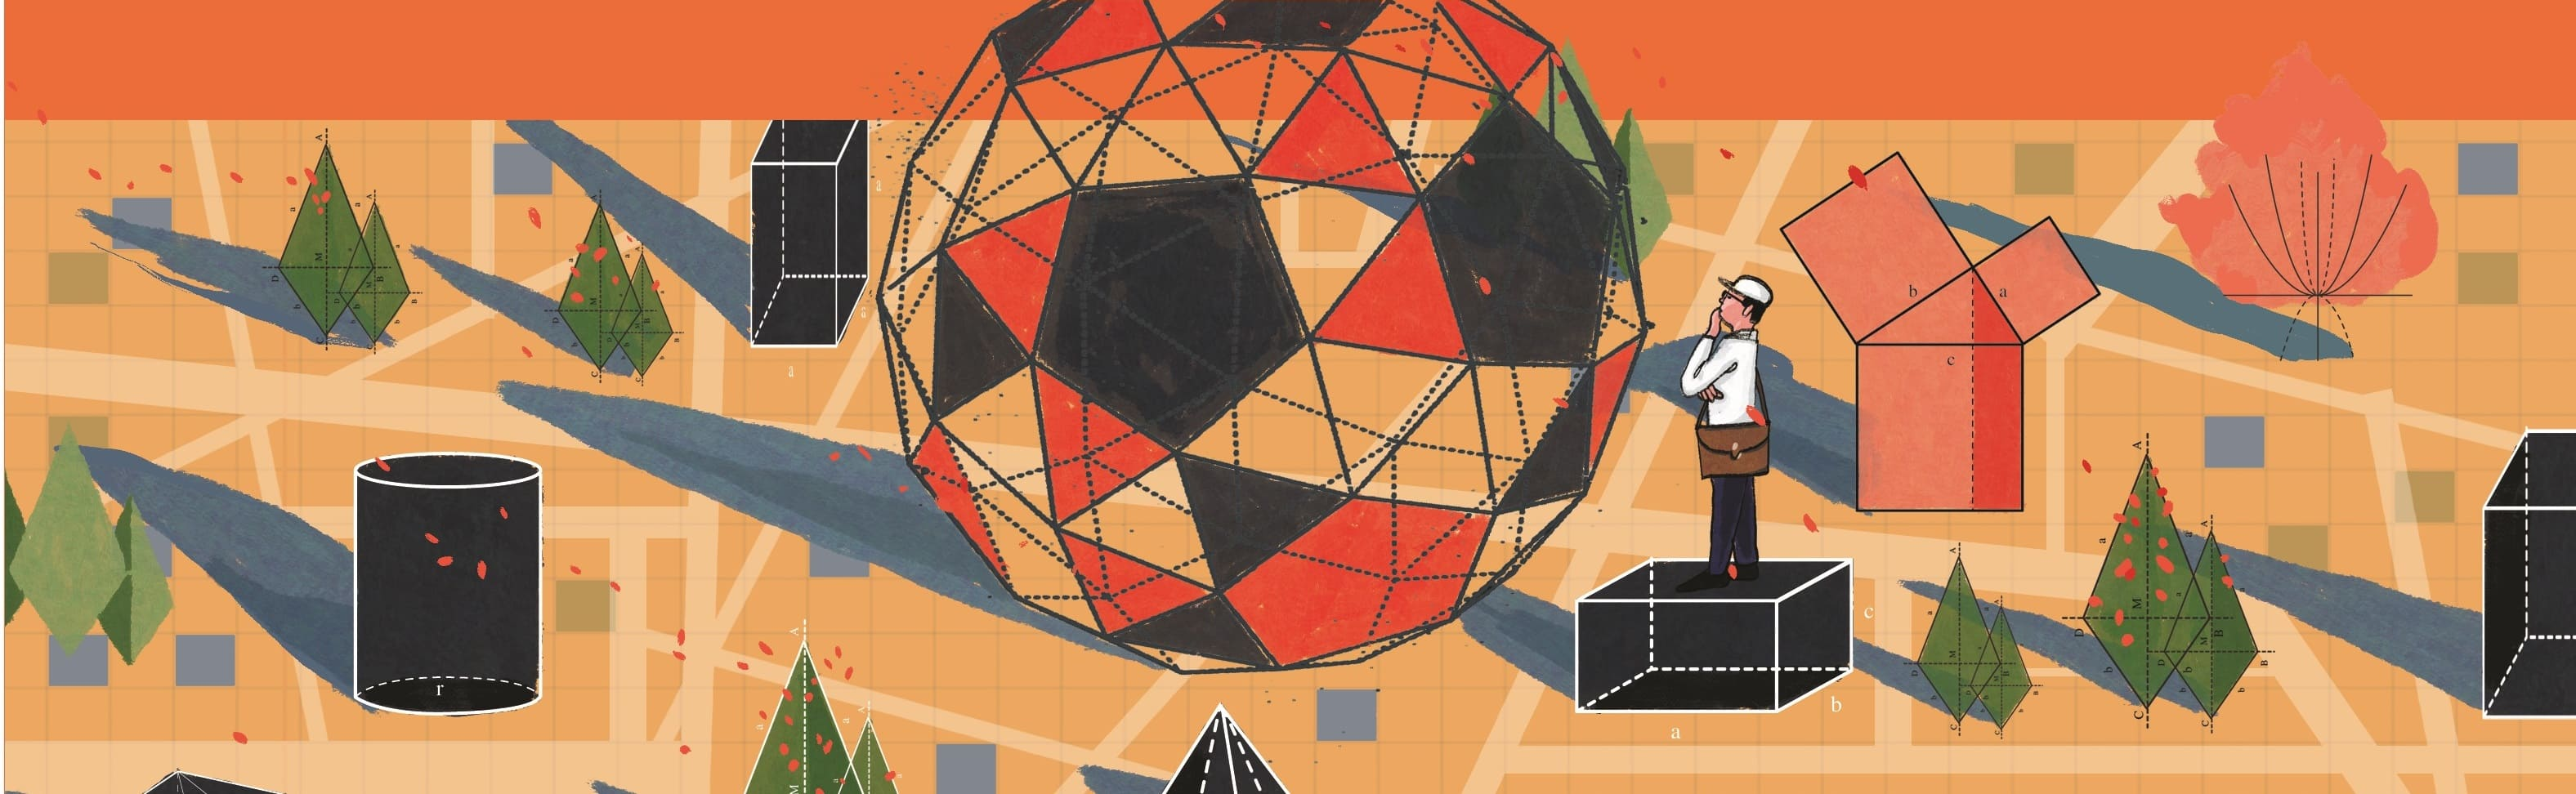
\includegraphics[width=19.3cm]{../bannerduongvao}}}
%\AddToShipoutPicture*{\put(138,522){
\includegraphics[scale=1]{../tieude.pdf}}}
\AddToShipoutPicture*{\put(130,522){
\includegraphics[scale=1]{../tieude1.pdf}}}
\centering
\endgroup

\vspace*{185pt}

\begin{multicols}{2}	
%	Đại hội Toán học thế giới (The International Congress of Mathematicians (ICM)) được tổ chức $4$ năm một lần là một sự kiện quan trọng của cộng đồng Toán học. Sau ``chiến dịch tranh cử'' của những nhà toán học Nga đứng đầu là hai Huy chương Fields A.~Okounkov và S.~K.~Smirnov, nước Nga đã giành quyền đăng cai. Nơi tổ chức Đại hội đã được ấn định từ trước là thành phố cổ kính Saint Petersburg từ ngày $6$ đến $14$ tháng $7$ năm $2022$. Tuy nhiên, vì một số yếu tố chính trị liên quan đến cuộc chiến giữa Nga và Ucraina, phiên họp trực tiếp đã không diễn ra, thay vào đó các báo cáo khoa học được để  dưới hình thức trực tuyến. Mặc dù vậy phiên họp Đại hội đồng của Liên đoàn Toán học thế giới nhằm bầu ra những vị trí chủ chốt của Liên đoàn Toán học thế giới nhiệm kỳ tiếp theo vẫn được tiến hành trực tiếp ở thủ đô Helsinki của Phần Lan với sự có mặt của các Chủ tịch hội toán học các nước. Tại phiên họp này các Huy chương Fields đã được trao vào ngày $5$ tháng $7$. Thực tế Helsinki cũng là nơi đăng cai Đại hội Toán học thế giới năm $1978$. Như chúng ta đã biết, ngoài điều kiện không quá $40$ tuổi, tiêu chí của Huy chương Fields là ``trao cho những khám phá xuất sắc trong Toán học đối với những công trình đặc biệt thú vị và hứa hẹn những khám phá tiếp theo''. Kết quả là $4$ Huy chương Fields năm $2022$ đã được trao cho các nhà toán học tài năng sau đây (lần lượt theo vần chữ cái): 
%	\vskip 0.1cm
%	$\bullet$ Hugo Duminil--Copin: Anh sinh năm $1985$ tại Pháp, là giáo sư tại Đại học Geneva, Thụy Sĩ, đồng thời cũng là giáo sư của Viện nghiên cứu cao cấp về Khoa học tự nhiên (Institut des Hautes Études Scientifiques--IHES), Cộng hòa Pháp . Anh được trao Huy chương Fields vì đã ``đã giải quyết những giả thuyết đã có từ lâu trong lý thuyết xác suất của hiện tượng chuyển pha trong Vật lý thống kê, đặc biệt là với số chiều $3$ và chiều~$4$".
%	\begin{figure}[H]
%		\centering
%		\vspace*{-5pt}
%		\captionsetup{labelformat= empty, justification=centering}
%		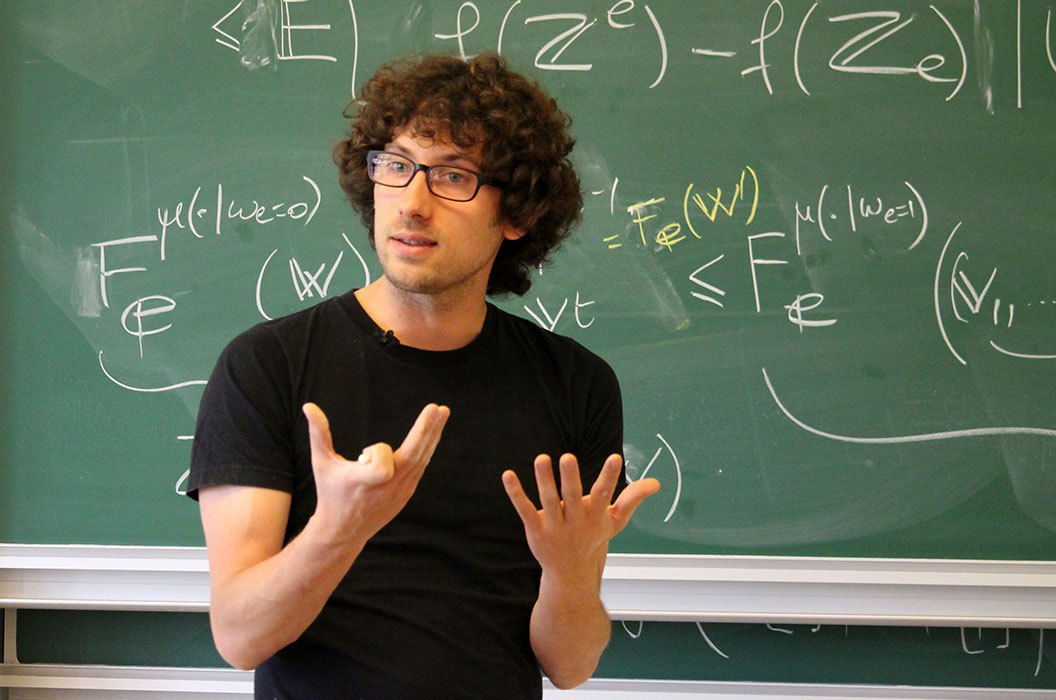
\includegraphics[width=1\linewidth]{Duminil-Copin}
%		\caption{\small\textit{\color{duongvaotoanhoc}Hugo Duminil--Copin.}}
%		\vspace*{-12pt}
%	\end{figure}
%	$\bullet$ June Huh: Anh sinh năm $1983$ tại Mỹ, nhưng là người Hàn Quốc và lớn lên cũng tại Hàn Quốc. Hiện anh là giáo sư tại Đại học\, Princeton,\, Hoa\, Kỳ.\, Anh\, nhận\, được\, Huy 
%	\end{multicols}
%	\begin{multicols}{2}
%	chương Fields vì ``việc mang những ý tưởng của lý thuyết Hodge vào tổ hợp, vì chứng minh giả thuyết Dowling--Wilson về các dàn hình học, chứng minh giả thuyết Heron--Rota--Welsh cho các matroids, và phát triển lý thuyết về các đa thức Lorentz, cùng với việc chứng minh giả thuyết Mason dạng mạnh".
%	\begin{figure}[H]
%		\centering
%		\vspace*{-5pt}
%		\captionsetup{labelformat= empty, justification=centering}
%		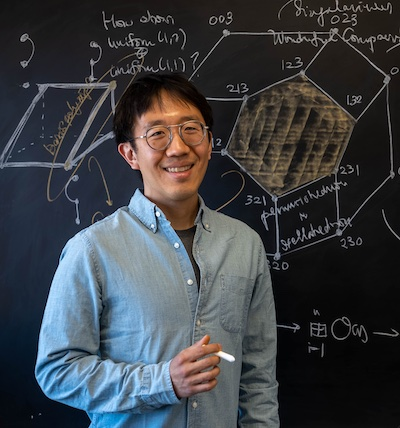
\includegraphics[width=1\linewidth]{Huh}
%		\caption{\small\textit{\color{duongvaotoanhoc}June Huh.}}
%		\vspace*{-10pt}
%	\end{figure}	
%	$\bullet$ James Maynard: Anh sinh năm $1987$ tại Vương Quốc Anh, là giáo sư tại Đại học Oxford. Huy chương Fields của J. Maynard
%	được trao cho việc đã có ``những đóng góp trong Lý thuyết số giải tích, dẫn đến những tiến bộ chính trong việc hiểu cấu trúc các số nguyên tố và trong xấp xỉ Diophantine". 
%	\vskip 0.1cm
%	$\bullet$ Maryna Viazovska: Chị sinh năm $1984$ tại Ucraina, là giáo sư đặc biệt (lãnh đạo nhóm Lý thuyết số) tại Đại học Bách Khoa Lausanne (EPFL), Thụy Sĩ. Chị được Huy chương Fields vì ``đã chứng minh được dàn $E_{8}$ cung cấp cách sắp xếp các hình cầu giống nhau một cách dày đặc nhất trong không không gian $8$ chiều, và những ứng dụng khác cho bài toán cực trị trong giải tích Fourier".
%	\vskip 0.1cm
%	Sau đây là một vài điểm chi tiết hơn một chút về công trình cũng như một vài thông tin khác của những nhà toán học nói trên. 
%	\begin{figure}[H]
%		\centering
%		\vspace*{5pt}
%		\captionsetup{labelformat= empty, justification=centering}
%		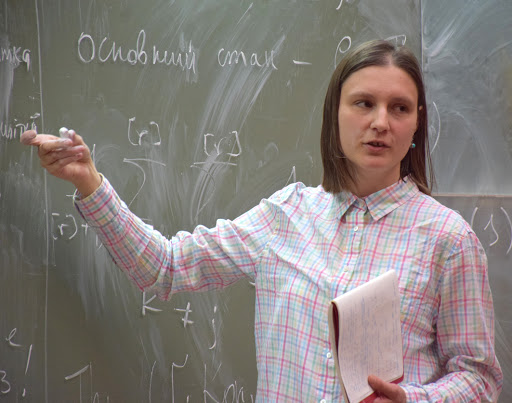
\includegraphics[width=1\linewidth]{Viazovska}
%		\caption{\small\textit{\color{duongvaotoanhoc}Maryna Viazovska.}}
%		\vspace*{-10pt}
%	\end{figure}
%	$1.$ Hugo Duminil--Copin: Anh được xem là đã làm thay đổi nền tảng toán học của hiện tượng chuyển pha trong Vật lý thống kê và đã giải quyết một số vấn đề mở đã có từ lâu trong Lý thuyết này, nói riêng trong trường hợp chiều $3$, chiều $4$ và trường hợp không khả tích khi số chiều bằng $2$. Chuyển pha là là một thuật ngữ mô tả sự chuyển tiếp các trạng thái của vật chất như rắn, lỏng, khí, plasma (ví dụ khi đun sôi đến $100$ độ C, dưới áp suất thông thường thì nước bắt đầu bay hơi). Mô hình Vật lý để mô tả những hiện tượng này là mô hình của E. Ising (một nhà Vật lý người Đức) trong Vật lý thống kê. Số chiều $2,3,4$ nói ở trên là số chiều của mô hình Ising. Công việc của Hugo Duminil--Copin là sự tiếp nối từ công việc của người thầy hướng dẫn của anh, Stanislav Smirnov (Huy chương Fields năm $2010$ về những đóng góp trong trường hợp số chiều $2$), cho những nền tảng toán học chặt chẽ để giải thích cho hiện tượng chuyển pha trong Vật lý nói trên thông qua mô hình Ising. Thực ra kết quả Toán học quan trọng đầu tiên về những mô hình Ising đã được L. Onsager (nhà bác học được giải Nobel về Hóa học năm $1968$) tìm ra. 
%	\vskip 0.1cm
%	Cần nói thêm rằng ngay từ khi làm luận án Tiến sĩ, Hugo đã có công trình quan trọng với thầy của mình giải quyết giả thuyết Nienhuis trong Vật lý thống kê về những hằng số liên kết cho những dàn lục giác. Chính kết quả này cũng đã góp phần tạo nên Huy chương Fields năm $2010$ của Stanislav Smirnov. Sau khi bảo vệ luận án Tiến sĩ năm $2013$, anh đã nhanh chóng trở thành chuyên gia hàng đầu về các khía cạnh xác suất của mô hình Ising. Bên cạnh mô hình Ising, Hugo còn có nhiều đóng góp cho mô hình Potts cũng trong Vật lý thống kê. Ở đây anh cùng với các cộng sự cũng đã giải quyết được một giả thuyết của Baxter đưa ra từ những năm $1970$. Vì những kết quả xuất sắc kể trên, khi chỉ ở độ tuổi $30$ anh đã là Giáo sư ĐH Geneve (Thụy Sĩ) và là Giáo sư ở Viện nghiên cứu cao cấp (Institut des Hautes Études Scientifiques (IHÉS)), Cộng hòa Pháp. Trước khi được trao Huy chương Fields, anh đã nhận được nhiều giải thưởng quan trọng như Giải thưởng của Hội Toán học Châu Âu, Giải thưởng của Viện hàn lâm khoa học Pháp, và một số giải thưởng của chuyên ngành Xác suất như giải thưởng Loeve, Dobrushin, ...  
%	\vskip 0.1cm
%	$2.$ James Maynard: Các công việc của anh được xem có tính độc đáo rất cao, thường dẫn đến những kết quả có tính đột phá đáng ngạc nhiên cho những vấn đề quan trọng, tưởng chừng như không thể thực hiện được với những kỹ thuật hiện tại.  
%	\begin{figure}[H]
%		\centering
%		\vspace*{-5pt}
%		\captionsetup{labelformat= empty, justification=centering}
%		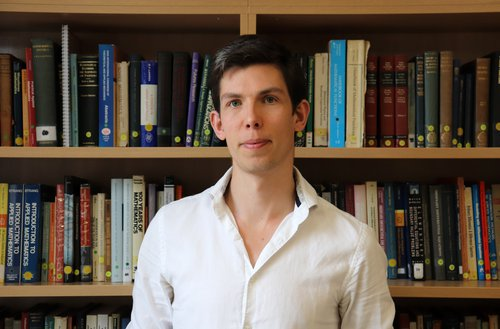
\includegraphics[width=1\linewidth]{Maynard}
%		\caption{\small\textit{\color{duongvaotoanhoc}James Maynard.}}
%		\vspace*{-10pt}
%	\end{figure}
%	Anh là một nhà Toán học người Anh, và được phong giáo sư ở Đại học Oxford danh tiếng vào năm $2017$ khi mới vừa tròn $30$ tuổi. Trước đó, anh làm dưới sự hướng dẫn của một trong những chuyên gia đầu ngành về Lý thuyết số giải tích là Roger Heath--Brown. Trước khi được trao Huy chương Fields, anh đã dành được một số giải thưởng quan trọng khác như giải thưởng SASTRA Ramanujan năm $2014$, giải thưởng Whitehead cho các nhà toán học trẻ của Hội Toán học London năm $2015$, giải thưởng của Hội toán học Châu Âu năm $2016$.    
%	\vskip 0.1cm
%	Như đã biết, số nguyên tố là một lĩnh vực cổ điển của Lý thuyết số mà không nhiều người dám thử sức vì khả năng có kết quả tương đối thấp. Ngoại trừ kết quả về vô hạn số nguyên tố có từ thời Eulid, mà chứng minh của nó chỉ vài dòng được giới thiệu trong chương trình cấp hai, thì các kết quả được xem là định lý về số nguyên tố đều có các chứng minh ít nhiều cần đến kiến thức ở bậc đại học trở lên và rất khó. Ở góc nhìn tổng thể về phân bố số nguyên tố, một trong những kết quả quan trọng mở đầu cho những ứng dụng của giải tích trong số nguyên tố là định lý của J. Hadamard và de vallee Poussin năm $1896$ (được dự đoán từ trăm năm trước đó bởi A--M. Legendre):
%	\vskip 0.1cm
%	\textbf{\color{duongvaotoanhoc}Định lý} $\pmb{1.}$ \textit{Với $\pi(n)$ là số lượng các số nguyên tố nhỏ hơn hay bằng $n$ thì} 
%	\begin{align*}
%		\lim_{n \to \infty} \frac{\pi(n)}{{\rm ln}n}=1.
%	\end{align*}
%	Liên quan đến phân bố các số nguyên tố thì dự đoán lớn nhất còn tồn tại có lẽ là giả thuyết Riemann về không điểm của hàm zeta. Bên cạnh đó, một mặt với số $n$ lớn tùy ý luôn tồn tại một dãy $n$ số liên tiếp gồm toàn hợp số (chẳng hạn $(n+1)!+2, (n+1)!+3, \ldots, (n+1)!+(n+1)$), nhưng {\it có thể có} những cặp số nguyên tố sinh đôi $(p,p+2)$ lớn tùy ý, chẳng hạn $(518807,518809)$. Đó chính là nội dung của câu hỏi về cặp số nguyên tố sinh đôi vẫn còn mở: 
%	\vskip 0.1cm
%	\textbf{\color{duongvaotoanhoc}Câu hỏi} $\pmb{1.}$
%		Tồn tại vô hạn cặp số nguyên tố sinh đôi $(p,p+2)$?
%	\vskip 0.1cm
%	Năm $2006$, một kết quả quan trọng theo hướng khẳng định giả thuyết về các cặp số nguyên tố sinh đôi của Goldston--Graham--Pintz--Yıldırım đã chỉ ra 
%	\vskip 0.1cm
%	\textbf{\color{duongvaotoanhoc}Định lý} $\pmb{2.}$ (Goldston--Graham--Pintz--Yıldırım, Proc. Japan Academy $2006$).
%	\textit{Ký hiệu $p_{n}$ là số nguyên tố thứ $n$ thì}
%	\begin{align*}
%		\liminf  \frac{p_{n+1}-p_{n}}{{\rm log}p_{n}}=0.
%	\end{align*}
%	Sau đó, vào năm $2013$ có một bước tiến rất ấn tượng của Y. Zhang như sau.
%	\vskip 0.1cm
%	\textbf{\color{duongvaotoanhoc}Định lý} $\pmb{3.}$ (Y. Zhang, Ann. Math. $179$ ($2014$), $1121$--$1174$).
%	\textit{Với một số $N$ nào đó nhỏ hơn $70$ triệu, tồn tại vô hạn cặp số nguyên tố sai khác $N$. }
%	\vskip 0.1cm
%	Cũng cần phải nói thêm Y. Zhang lúc đó chỉ là một giảng viên Toán bình thường ở Đại học New Hampshire. Đây không hẳn là một đại học nghiên cứu (có đào tạo bậc Tiến sĩ về Toán), ở vùng Đông Bắc nước Mỹ. Sở dĩ ông công tác ở một đại học nhỏ như vậy vì kết quả chính trong luận án Tiến sĩ của mình tuy được công bố ở một tạp chí uy tín cao là Duke Math. J. nhưng đã sử dụng một kết quả mà sau này người ta mới biết là sai. Tuy kết quả năm $2014$ của Y. Zhang rất ấn tượng nhưng sau đó đã được làm mạnh hơn rất nhiều bởi James Maynard và nhóm của T. Tao (một nhà toán học rất nổi tiếng, Huy chương Fields năm $2006$) và các cộng sự. Điển hình là kết quả sau giảm số $70$ triệu của định lý trước của Y. Zhang xuống còn $600$:
%	\vskip 0.1cm
%	\textbf{\color{duongvaotoanhoc}Định lý} $\pmb{4.}$ (James Maynard, Ann. Math. ($2015$), vol. $181$ (no.$1$) $383$--$413$, nhóm của T. Tao cũng cho một chứng minh độc lập).
%	\textit{Ký hiệu $p_{n}$ là số nguyên tố thứ $n$ thì}
%	\begin{align*}
%		\liminf (p_{n+1}-p_{n}) \leq 600. 
%	\end{align*}
%	\textit{Nếu thừa nhận giả thuyết Elliot--Halberstam thì} 
%	\begin{align*}
%		\liminf (p_{n+1}-p_{n}) \leq 12,
%	\end{align*}
%	\textit{và}
%	\begin{align*}
%		\liminf(p_{n+2}-p_{n}) \leq 600. 
%	\end{align*}
%	Phương pháp mà James Maynard sử dụng phát triển phương pháp ``sàng'' của nhóm tác giả D. A. Goldston, J. Pintz, C. Y. Yildirim (Ann. Math. $2009$). Gốc rễ của phương pháp này chính là sàng Eratosthenes có từ thời cổ đại dùng để lọc ra các số nguyên tố nhỏ hơn một số cho trước. Ngoài kết quả có tính đột phá kể trên, J. Maynard cũng đã có những đóng góp cơ bản trong xấp xỉ Diophantine, cùng với Koukoulopoulos anh đã giải quyết Giả thuyết Duffin--Schaeffer (Ann. Math $2020$). Giả thuyết này được đưa ra năm $1941$, mô tả việc một số thực có thể được xấp xỉ tốt bởi một số hữu tỷ đến mức độ nào, và bắt nguồn từ bổ đề xấp xỉ nổi tiếng của Dirichlet. 
%	\vskip 0.1cm
	$3.$ June Huh: Anh được xem là đã cùng với một số cộng sự làm thay đổi lĩnh vực hình học tổ hợp thông qua việc dùng các phương pháp của lý thuyết Hodge (phương pháp để nghiên cứu đối đồng điều của những đa tạp Kahler compact), hình học nhiệt đới (tropical), và lý thuyết kỳ dị. Đối tượng tổ hợp chính mà June Huh quan tâm là các matroids. Matroid là một đối tượng gần với ma trận (matrix) và lý thuyết đồ thị, và lý thuyết về chúng có cảm hứng từ việc trừu tượng hóa nhiều khái niệm từ hai lý thuyết nói trên. Cụ thể hơn, matroid $M$ là một cặp $(E,\pazocal{I})$ gồm một tập hữu hạn $E$ và một họ $\pazocal{I}$ khác rỗng các tập con của $E$ thỏa mãn đồng thời $2$ điều kiện:
	\vskip 0.1cm
	$\bullet$ Nếu tập con $A$ của $E$ thuộc họ $\pazocal{I}$ thì mọi tập con của nó cũng thuộc $\pazocal{I}$.
	\vskip 0.1cm
	$\bullet$ Nếu $A, B \in \pazocal{I}$ và $|A| = |B| +1$, thì tồn tại một phần tử $x \in A \setminus B$ sao cho $B \cup \{x\} \in \pazocal{I}$.
	\vskip 0.1cm
	Mô hình cụ thể của một matroid là một ma trận với các cột đánh số bởi tập $E$ và họ $\pazocal{I}$ các tập con mà các cột ứng với tập con đó là độc lập tuyến tính.
	\vskip 0.1cm
	Đây là một khái niệm đưa ra bởi một nhà hình học nổi tiếng của thế kỷ trước là H. Whitney sau đó được phát triển nhiều bởi một chuyên gia nổi tiếng về tổ hợp là G--C. Rota. Sau này matroids tìm thấy nhiều ứng dụng trong hình học, tôpô, tổ hợp, ...
	\vskip 0.1cm
	Bên cạnh đó, hình học nhiệt đới (tropical) là một biến thể của hình học đại số. Trong khi hình học đại số nghiên cứu những đa tạp đại số là tập nghiệm của một hệ phương trình đa thức thì hình học nhiệt đới thay phép cộng trong đa thức bởi phép lấy giá trị nhỏ nhất và phép nhân thay bằng phép cộng. Ngay trong hình học đại số, lý thuyết hình học mới này đã có nhiều ứng dụng thông qua các công trình của M. Kontsevich (Huy chương Fields năm $1998$) và G. Mikhalkin. Tuy xuất phát từ hình học đại số nhưng theo nhận xét của June Huh các đa tạp nhiệt đới rộng hơn nhiều so với việc lấy nhiệt đới hóa (tropicalization) các đa tạp đại số, qua đó cho thấy những nghiên cứu của June Huh chắc sẽ còn hứa hẹn nhiều kết quả quan trọng.  
	\vskip 0.1cm
	Cụ thể hơn những công trình quan trọng làm nên Huy chương Fields của June Huh bao gồm:
	\vskip 0.1cm
	$\bullet$ June Huh đã cùng với Boton Wang sử dụng Hình học đại số và lý thuyết giao để chứng minh giả thuyết Dowling--Wilson về nhận biết các matroids. 
	\vskip 0.1cm
	$\bullet$ Karim Adiprasito, June Huh, và Eric Katz đã tìm ra một dạng tương tự của lý thuyết Hodge và chứng minh định lý Lefschetz dạng mạnh và quan hệ Hodge--Riemann cho các matroids tùy ý. Họ đã dùng các kết quả này để giải quyết giả thuyết Heron--Rota--Welsh về tính lõm loga của đa thức đặc trưng của một matroid. 
	\vskip 0.1cm
	$\bullet$ Petter Branden và June Huh đã phát triển lý thuyết về các đa thức Lorentz, liên hệ với giải tích lồi và phiên bản rời rạc của nó thông qua hình học nhiệt đới. Họ đã chứng minh giả thuyết Mason dạng mạnh cho các matroids và tìm ra các ứng dụng khác nhau từ hình học đại số xạ ảnh cho tới mô hình Potts trong cơ học thống kê (đã được đề cập đến trong công việc của Hugo Duminil--Copin).
	\vskip 0.1cm 
	June Huh có một quá trình đào tạo về Toán không thật chính quy. Anh tự nhận không giỏi Toán khi học phổ thông và học cả chuyên ngành Vật lý ở bậc đại học ở Đại học Quốc Gia Seoul (Hàn Quốc) nhưng bảng điểm không thật tốt. Đến những năm cuối đại học, anh được tham dự các bài giảng về Hình học đại số của H. Hironaka (Huy chương Fields năm $1970$ của Nhật Bản, nổi tiếng với định lý giải kỳ dị) khi ông là Giáo sư mời của Đại học Quốc gia Seoul. Lúc này anh bắt đầu có cảm hứng và bắt đầu dành nhiều thời gian hơn cho Toán học. Tốt nghiệp Đại học xong, anh làm luận văn Thạc sĩ với một trong những chuyên gia hàng đầu về Hình học đại số của Hàn Quốc là Young--Hoon Kiem. Sau đó, năm $2009$, anh được nhận làm luận án Tiến sĩ Toán ở Mỹ, ban đầu là Đại học Illinois ở Urbana--Champaign, sau đó chuyển sang Đại học Michigan. Anh bảo vệ luận án Tiến sĩ năm $2014$ dưới sự hướng dẫn của một chuyên gia nổi tiếng về Hình học đại số là M. Mustata. Tuy bắt đầu làm luận án Tiến sĩ khá muộn, nhưng ngay từ những năm đầu khi làm luận án Tiến sĩ, anh đã dùng những kỹ thuật của hình học đại số để chứng minh giả thuyết Read về hệ số của đa thức sắc số (chromatic polynomials) trong lý thuyết đồ thị. Đây là một giả thuyết từ hơn $40$ năm trước xuất phát từ bài toán $4$ màu nổi tiếng mà lời giải của nó dài vài trăm trang được đưa ra bởi K. Appel và W. Haken năm $1976$ cùng với sự hỗ trợ của máy tính. Bài báo của June Huh ngay lập tức đã được chú ý và in ở một tạp chí hàng đầu là Journal of the American Mathematical Society. Một điều thú vị là chính trong bài báo này, June Huh cũng đã trả lời một câu hỏi liên quan của GS. Ngô Việt Trung và J. K. Verma về số bội trộn trong Đại số giao hoán. Nhờ những kết quả quan trọng trong luận án, anh được nhận học bổng nghiên cứu danh giá của Viện Clay, và nhận vị trí Veblen Instructor, cũng như vị trí giáo sư mời ở Viện nghiên cứu cao cấp Princeton. Đến năm $2020$, anh nhận vị trí giáo sư ở Đại học Stanford, nhưng chỉ $1$ năm sau đó anh quay lại nhận vị trí giáo sư ở Đại học Princeton.     
	\vskip 0.1cm
	$4.$ Maryna Viazovska: Như đã nói ở trên được trao huy chương Fields một phần vì những đóng góp trong bài toán xếp hình cầu.
	\vskip 0.1cm
	Một vấn đề có từ lâu trong toán học là tìm một cách sắp xếp dày đặc nhất (tối ưu nhất) những hình cầu giống nhau trong không gian với số chiều cho trước. Dày đặc nhất ở đây hiểu là tỷ lệ giữa tổng thể tích các hình cầu và thể tích hình chứa nó là lớn nhất. Bài toán này cũng rất tự nhiên trong thực tế khi ta đi du lịch và cần phải xắp xếp sao cho balo chứa được nhiều đồ vật nhất. Ở chiều $2$ ta biết cách sắp xếp theo hình lục lăng (một hình tròn ở giữa, $6$ hình tròn đặt xung quanh trong một lục giác đều) cho ta cách xếp dày đặc nhất. Với số chiều $3$, từ vài trăm năm trước, J. Kepler đã dự đoán cách xếp các quả cam chứa trong một hình kim tự tháp sẽ cho kết quả tối ưu. Năm $1998$, T. Hales chứng minh giả thuyết Kepler với một chứng minh gần $100$ trang in ở Annals of Mathematics cùng với sự trợ giúp của máy tính. Bài toán sắp xếp hình cầu không có thêm kết quả gì ở các số chiều khác cho đến năm $2016$, M.~Viazovska chỉ ra dàn $E_{8}$ (dàn (lưới) trong không gian $\mathbb{R}^8$, liên quan đến nhóm Lie dạng $E_{8}$) cho cách xếp tối ưu nhất trong chiều $8$. Ít lâu sau đó cùng với H. Cohn, A. Kumar, S. Miller và D. Radchenko, M.~Viazovska đã chứng minh dàn Leech cho cách sắp xếp dày đặc nhất ở số chiều $24$. Dàn Leech nằm trong không gian $\mathbb{R}^{24}$ có nhóm các tự đẳng cấu là nhóm đơn hữu hạn loại lẻ tẻ (sporadic) đưa ra bởi Conway. Lời giải của M.~Viazovska dựa trên cách tiếp cận của H. Cohn và N.~Elkies (Ann. Math. $2003$), những người đã dùng công thức tổng Poisson của giải tích điều hòa để tìm ra một chặn trên cho những khả năng có thể có của mật độ cho bài toán xếp cầu với số chiều tùy ý. Công trình của các nhà toán học này cần đến sự tồn tại của những hàm Schwatz với những tính chất đặc biệt (chẳng hạn hàm đó và biến đổi Fourier của nó triệt tiêu tại những giá trị độ dài của vectơ trong các dàn tương ứng). H. Cohn và N.~Elkies nghĩ rằng những hàm có tính chất đặc biệt như thế là tồn tại nhưng chưa có ý tưởng gì để xây dựng. Khi công việc dừng ở đó khoảng $10$ năm thì M.~Viazovska xuất hiện và đưa ra một phương pháp hoàn toàn mới để đưa ra những hàm này dựa trên lý thuyết về các dạng modular. Như chúng ta đã biết các dạng modular là một lĩnh vực thuộc Lý thuyết số hiện đại và cung cấp những điểm mấu chốt cho lời giải bài toán Fermat của A. Wiles từ khoảng gần $30$ năm trước. Sau đó kỹ thuật chọn hàm Schwatz dùng dạng modular cũng đã được H. Cohn khai thác và thu được những kết quả quan trọng gần đây. Việc dùng các dạng modular là một đối tượng rất khác để giải quyết vấn đề nói trên ít nhiều có sự hợp lý nếu chúng ta nhìn vào đào tạo của M.~Viazovska. Ngay từ phổ thông, chị đã là một học sinh giỏi Toán, tốt nghiệp Đại học ở Ucraina, sau đó làm luận văn cao học Đức, rồi quay lại Ucraina làm luận án Tiến sĩ và bảo vệ vào năm $2010$. Sau đó chị sang Đức làm luận án Tiến sĩ với một trong hai người thầy hướng dẫn là Don Zagier, một chuyên gia về nhiều thứ trong đó có lý thuyết các dạng modular. Một điều đáng ngạc nhiên là mặc dù lời giải bài toán xếp cầu trong trường hợp $3$ chiều rất dài và cần đến máy tính kiểm tra nhưng lời giải trong trường hợp $8$ chiều và $24$ chiều lại khá ngắn gọn (khoảng $20$ trang). Vì những kết quả độc đáo này, M.~Viazovska đã nhận được giải thưởng nghiên cứu của Viện Clay năm $2017$ dành cho những kết quả Toán học xuất sắc nhất trong năm.        
	\vskip 0.1cm
	Sau lời giải bài toán xếp cầu ở chiều $8$ và $24$, M.~Viazovska đã phát triển tiếp tục ý tưởng của riêng mình. Chị đã cùng với D.~Radchenko ($2019$) chứng minh mọi hàm Schwatz chẵn thỏa mãn hàm đó cùng với biến đổi Fourier triệt tiêu tại các số $\sqrt{n}$ ($n$ là số nguyên không âm) luôn đồng nhất bằng $0$. Kết quả này được các chuyên gia đánh giá là rất đáng ngạc nhiên.
	\vskip 0.1cm
	{\bf\color{duongvaotoanhoc} Kết luận:}  Từ những phân tích kể trên ta thấy đóng góp của những giải thưởng Fields luôn rất đặc biệt, thường là lời giải cho những vấn đề quan trọng, và lời giải nhiều khi đến từ những lĩnh vực hoàn toàn khác.
	\vskip 0.1cm
	\textbf{\color{duongvaotoanhoc}Tài liệu tham khảo}
	\vskip 0.1cm
	[$1$] Trang web \url{https://www.mathunion.org/imu-awards/fields-medal/fields-medals}\\ \url{-2022}
	\vskip 0.1cm
	[$2$] Các trang wikipedia.
\end{multicols}
 
%	\newpage
%	
%	 \setcounter{figure}{0}
%	 \thispagestyle{quantoannone}
\pagestyle{quantoan}
\everymath{\color{quantoan}}
\graphicspath{{../quantoan/pic/}}
\blfootnote{\color{quantoan}\color{quantoan}$^*$Nguồn Math. Intellegencer, Số $41$.}
\begingroup
\AddToShipoutPicture*{\put(0,616){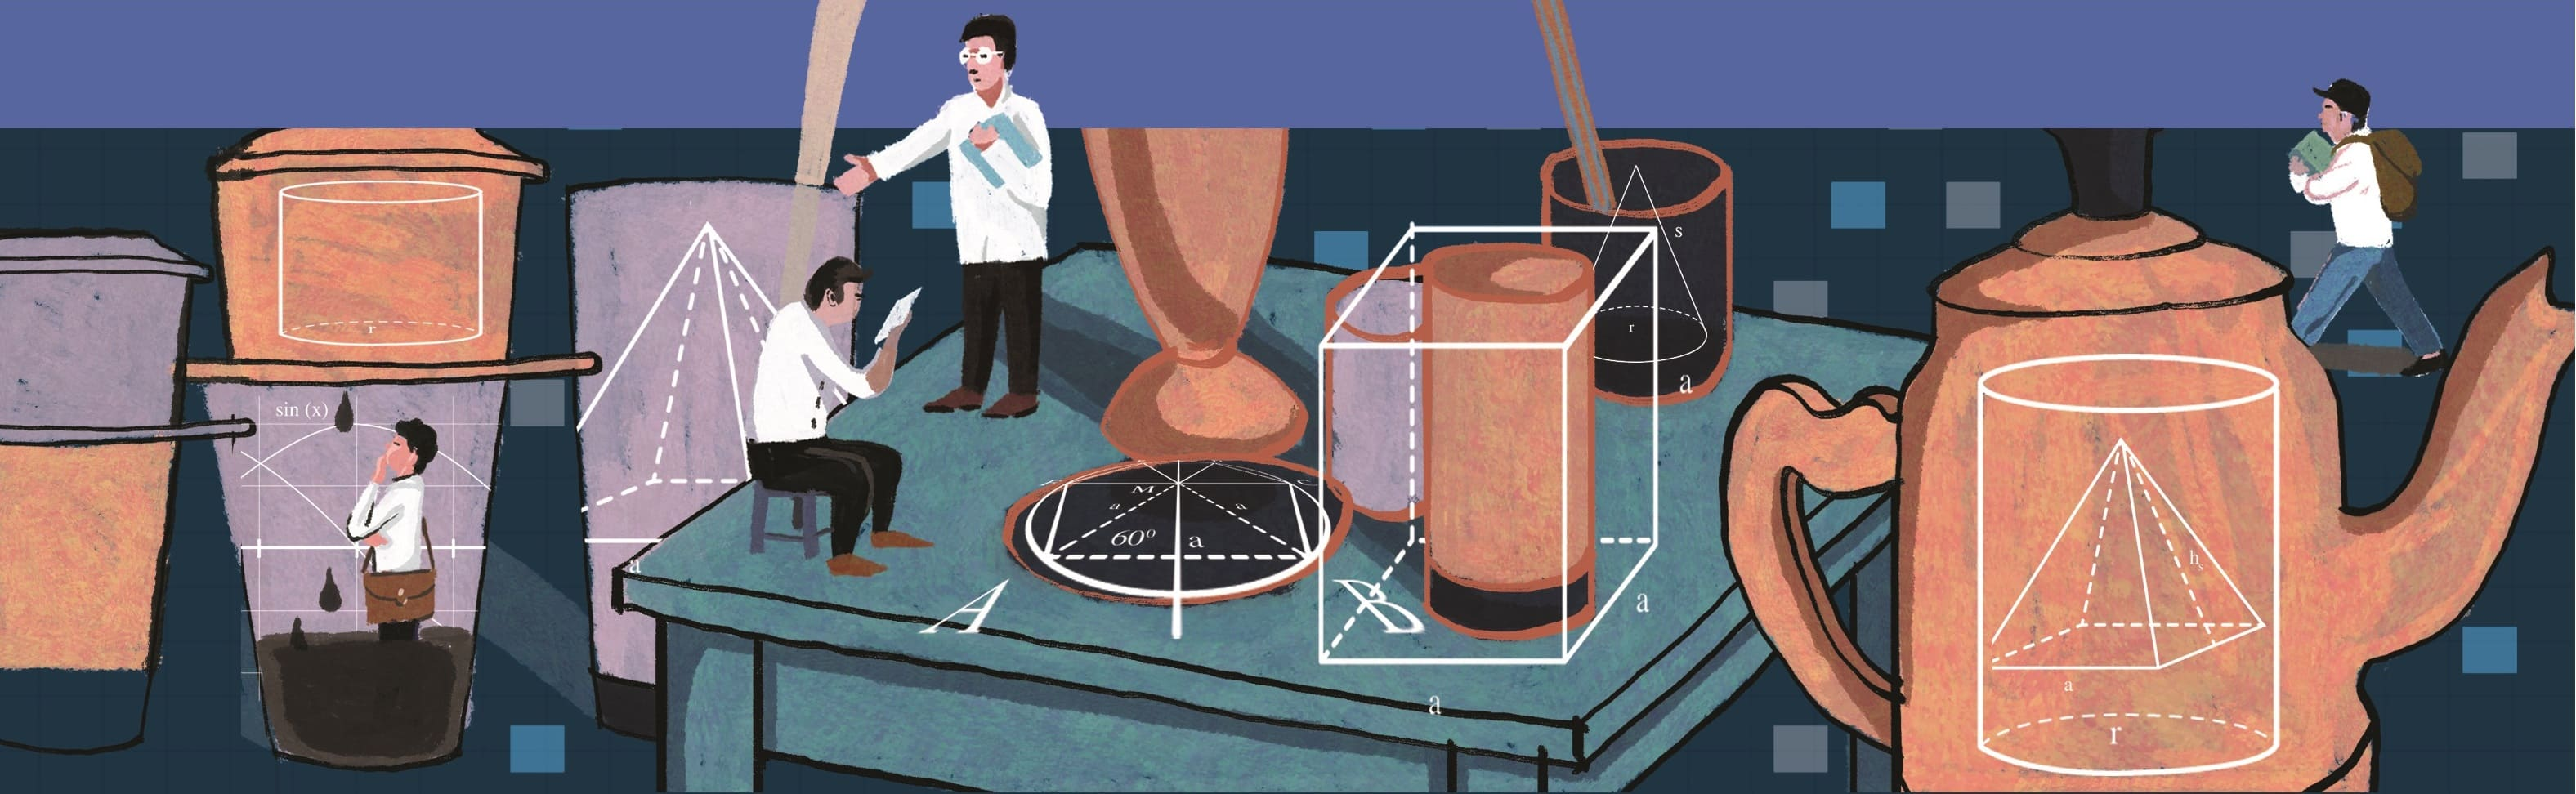
\includegraphics[width=19.3cm]{../bannerquantoan}}}
\AddToShipoutPicture*{\put(58,505){
\includegraphics[scale=1]{../tieude.pdf}}}
\centering
\endgroup

\vspace*{198pt}

\begin{multicols}{2}
	Ai cũng biết rằng Charles Lutwidge Dodgson (bút danh Lewis Carroll, $1832-1898$; Hình $1$), tác giả của \textit{Alice ở xứ xở diệu kỳ}, là một nhà toán học. Dodgson là một giảng viên toán tại trường Christ Church thuộc Đại học Oxford và đã có nhiều công trình toán học về hình học, đại số, logic và lý thuyết bỏ phiếu. Hầu hết mọi đánh giá về toán học của Dodgson đều nhắc đến một câu chuyện thú vị (sau đây gọi là \textit{câu chuyện}) liên quan đến nữ hoàng Victoria. Nữ hoàng được cho là rất thích truyện \textit{Alice}, xuất bản năm $1865$, và đã yêu cầu tác phẩm tiếp theo của tác giả. Với sự ngạc nhiên và thất vọng, bà đã nhận được cuốn \textit{Chuyên luận về định thức} của Dodgson, xuất bản năm $1867$. Câu chuyện này là một giai thoại kinh điển mà người ta thường bắt gặp trong các tác phẩm về toán học.
	\vskip 0.02cm
	Những bài viết về \textit{câu chuyện} cũng đôi khi nhắc nhở chúng ta rằng chính Dodgson đã phủ nhận nó vào năm $1896$, nhưng sự lan rộng của tin đồn dường như không thể ngăn được. Có thể dễ dàng hiểu được sức hấp dẫn của nó, vì nó thể hiện một cách hoàn hảo quan niệm rộng rãi về Dodgson nói riêng và toán học nói chung. Đầu tiên, câu chuyện truyền tải một cái nhìn rộng rãi về Dodgson như một nhân vật kép: một mặt là nhà toán học buồn tẻ và mặt khác là một tiểu thuyết gia giàu trí tưởng tượng. Thứ hai, phản ứng được cho là của nữ hoàng tiêu biểu cho niềm tin rằng toán học và văn học bắt nguồn từ những bộ óc và nền văn hóa khác nhau. Điều thú vị là nhiều lời kể về \textit{câu chuyện} nói rằng nữ hoàng không hài lòng khi nhận được cuốn sách. Người ta cũng nói rằng Dodgson, người rất tôn kính hoàng gia, không thể nào thực hiện một ``hành động hoàn toàn ngược với tính cách" như vậy (Beale $1973$). Nhưng  tặng một cuốn sách toán cho nữ hoàng thì có gì sai?  
	\begin{figure}[H]
		\vspace*{-5pt}
		\centering
		\captionsetup{labelformat= empty, justification=centering}
		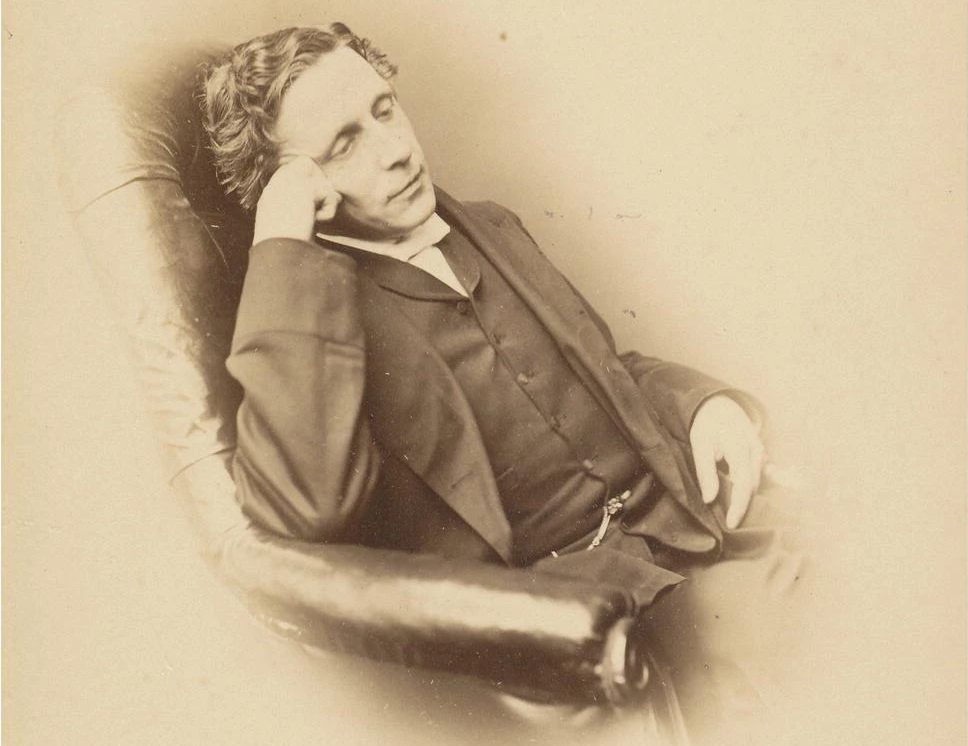
\includegraphics[width= 1\linewidth]{1}
		\caption{\small\textit{\color{quantoan}Hình $1$. Charles L. Dodgson (from the Wakeling
				Collection).}}
		\vspace*{-5pt}
	\end{figure}
	\textbf{\color{quantoan}Câu chuyện lan truyền chóng mặt}
	\vskip 0.1cm
	Khi \textit{Alice ở xứ xở diệu kỳ} ra mắt (Dodgson $1865$, Hình $2$), Dodgson là một tác giả vô danh. Ông mới chỉ xuất bản một số tập sách nhỏ về toán học và các tác phẩm nhỏ. Đặc biệt, vào năm $1856$, ông đã đóng góp một số bài thơ cho tạp chí \textit{Chuyến tàu}, ở đó ông sử dụng bút danh Lewis Carroll, lấy từ tên của mình (Lewis từ Lutwidge và Carroll từ Charles). Những năm sau đó, ông chủ yếu sử dụng tên thật cho các công trình toán học và bút danh cho các tác phẩm văn học để giữ kín danh tính của mình. Thành công tức thì của cuốn sách \textit{Alice} đã làm cho bút danh văn học của ông được đông đảo công chúng biết đến, nhưng họ không biết được ông có thể là ai.
	\begin{figure}[H]
		\vspace*{-5pt}
		\centering
		\captionsetup{labelformat= empty, justification=centering}
		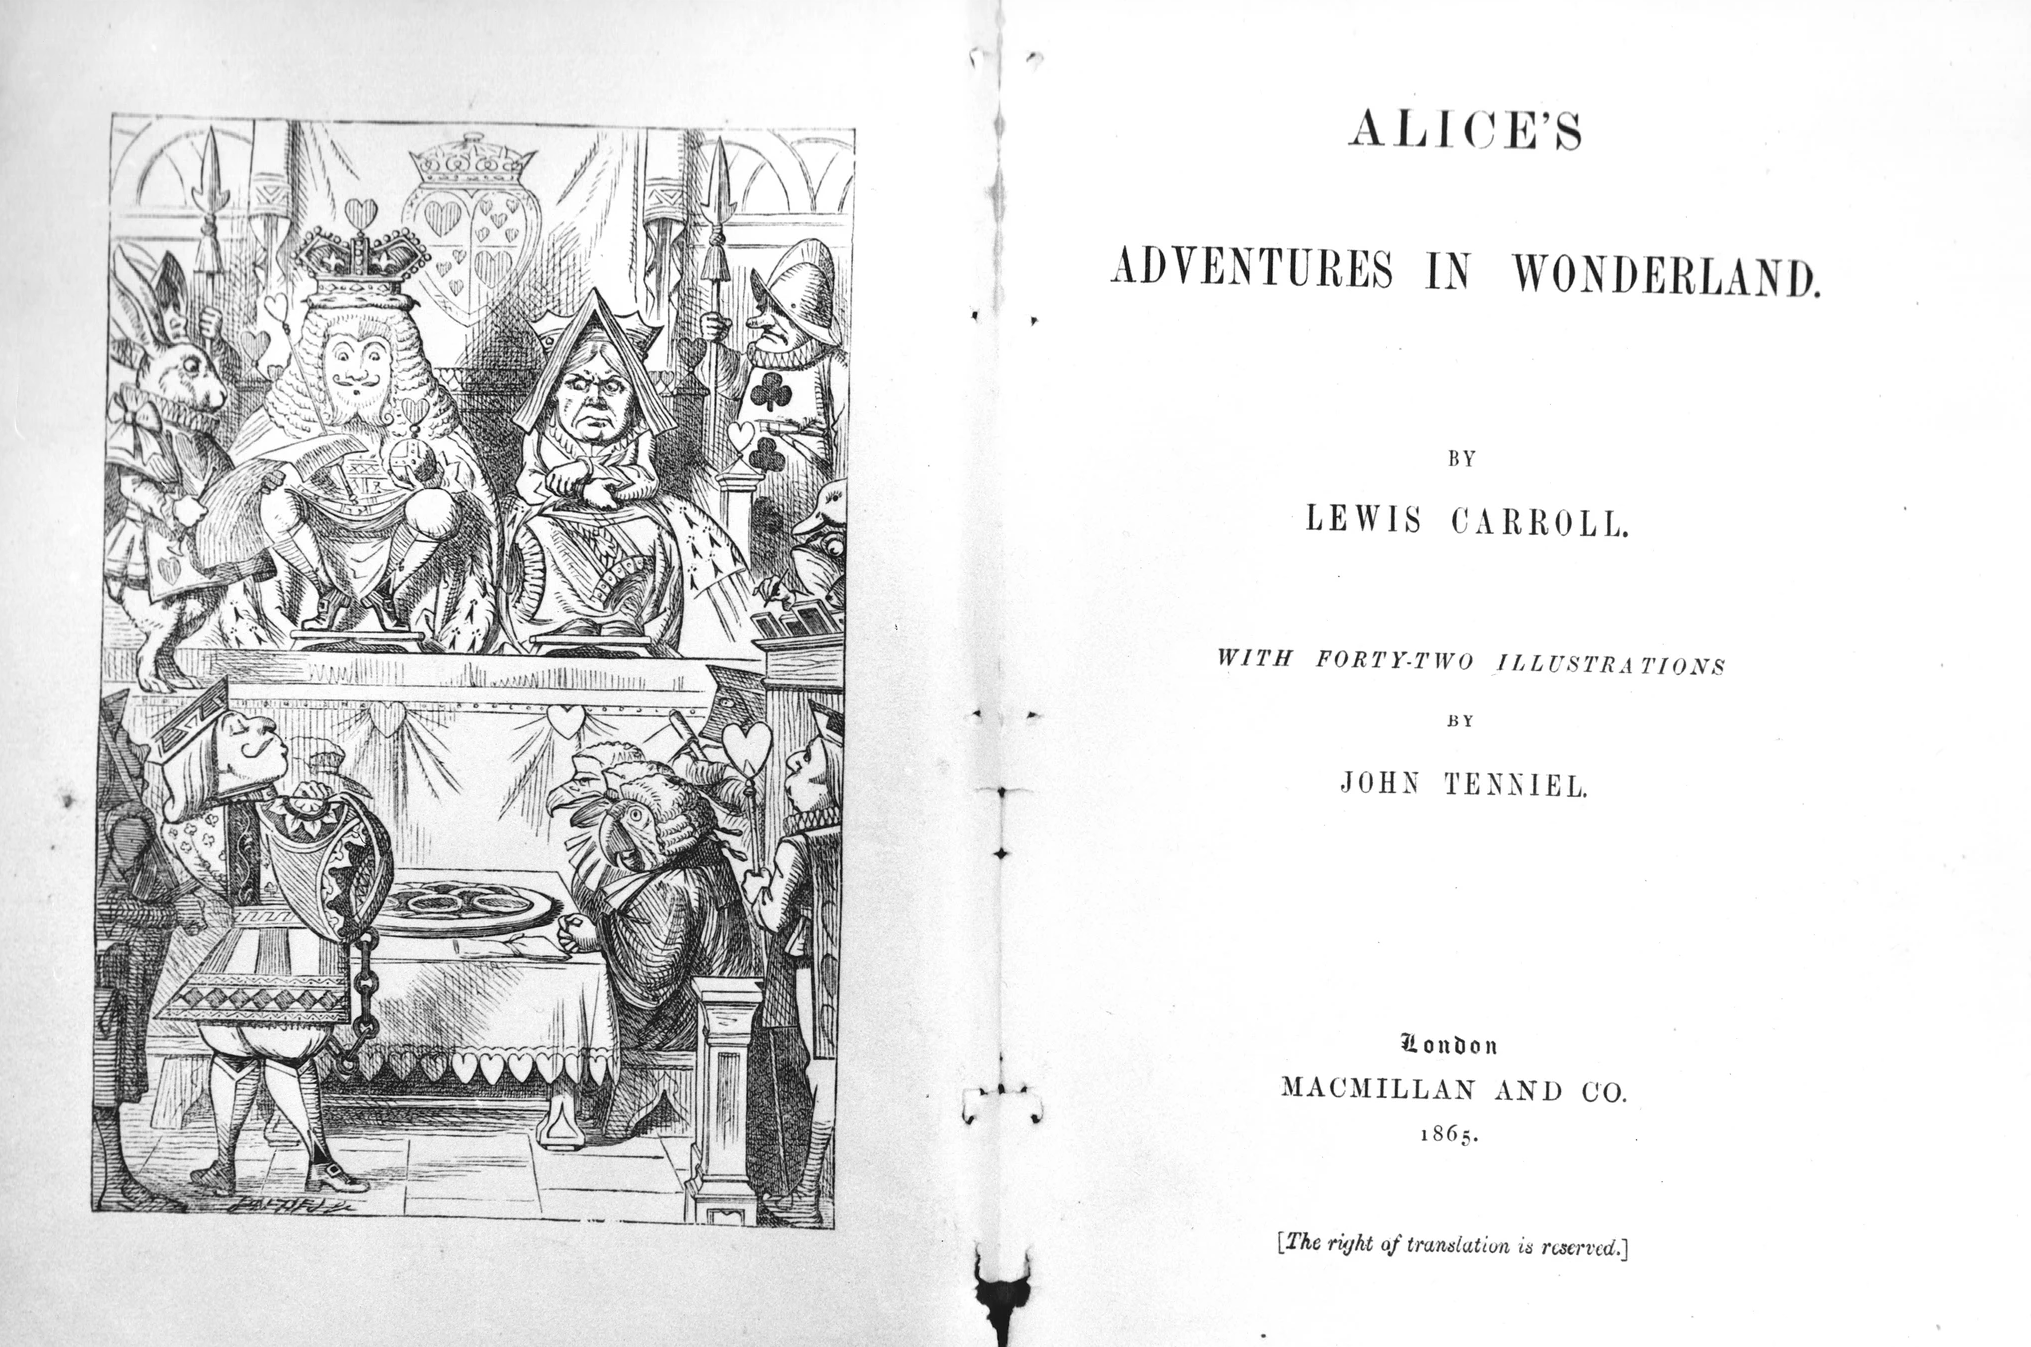
\includegraphics[width= 1\linewidth]{2}
		\caption{\small\textit{\color{quantoan}Hình $2$. The title page of Dodgson’s Alice’s Adventures in Wonderland, $1865$ (Photo by George Bayntun, Collection of Charlie Lovett).}}
		\vspace*{-10pt}
	\end{figure}
	Cuốn sách cũng được hưởng một nỗ lực quảng bá lớn của cả nhà xuất bản và tác giả. Vô số các bản sao đã được gửi đến các tạp chí để đánh giá, hoặc tặng bạn bè làm quà. Cháu trai, đồng thời là người viết tiểu sử đầu tiên của Dodgson, Stuart D. Collingwood, đã thuật lại rằng bản sao đầu tiên của cuốn sách được gửi đến Alice ngoài đời thực, người đã truyền cảm hứng cho câu chuyện, còn bản thứ hai được gửi đến công chúa Beatrice, con gái út của nữ hoàng Victoria (Collingwood $1898$, tr.$104$) . Đáp lại, Dodgson nhận được một lá thư cho biết ``cuốn sách nhỏ mà Bệ hạ rất hài lòng khi cho phép đọc nó cho công chúa Beatrice" (Wakeling $1999$, tr. $122$).
	\vskip 0.1cm
	Với sự khen ngợi của giới phê bình và số lượng lớn sách bán được, ý tưởng về phần tiếp theo hẳn đã nhanh chóng nảy ra với Dodgson và nhà xuất bản của ông. Ngay từ năm $1866$, Dodgson đã đề cập đến việc ``đang cân nhắc ý tưởng về việc viết một thứ kiểu như phần tiếp theo". Công chúng rõ ràng đã mơ màng về những cuộc phiêu lưu khác, và có tin đồn rằng ``Lewis Carroll đang viết tiếp" (Collingwood $1898$, tr.$129$).
	\vskip 0.1cm
	Quả thực là Dodgson đang viết. Bên cạnh những thứ khác, ông đang nghiên cứu về thứ có thể là đóng góp quan trọng nhất của ông cho nghiên cứu toán học. Thật vậy, ông đã đưa ra một phương pháp mới để tính toán các định thức, trình bày nó trước Hiệp hội Hoàng gia Luân Đôn vào tháng $5$ năm $1866$, và sau đó công trình này xuất hiện trong Kỷ yếu của Hiệp hội Hoàng gia Luân Đôn. Trong vòng một năm sau đó, Dodgson đã phát triển bài báo của mình thành một ``cuốn sách nhỏ", mà ông ghi lại trong nhật ký của mình là ``đã mang lại cho [ông] nhiều rắc rối hơn bất cứ thứ gì mà ông đã từng viết" (Wakeling $1999$, $206-207$). Việc xuất bản cuốn sách bị gián đoạn bởi một chuyến đi đến nước Nga cùng với Henry Parry Liddon từ tháng $7$ đến tháng $9$ năm $1867$. \textit{Chuyên luận về định thức} cuối cùng được xuất bản vào đầu tháng $12$ năm đó (Hình $3$). Cuốn sách này đã nhận được một số lời khen ngợi về đóng góp và tính mới, nhưng bị chỉ trích vì văn phong logic nặng nề và sự lựa chọn thuật ngữ và ký hiệu gây khó đọc.
	\vskip 0.1cm
	\textit{Chuyên luận về định thức} là cuốn sách đầu tiên của Dodgson kể từ Alice, nhưng nó không có liên hệ gì với cuốn truyện tuyệt vời đó. Trước khi hoàn thành, Dodgson đã thông báo cho nhà xuất bản của mình, Macmillan, trong một bức thư ngày $11$ tháng $2$ năm $1867$, về ý định đề tên thật của mình cho cuốn sách: ``Tôi có một cuốn sách nhỏ, sắp hoàn thành, mà tôi muốn các ông xuất bản cho tôi -- nhưng tôi e rằng nó không thể được giới thiệu như là của tác giả 'của \textit{Những cuộc phiêu lưu của Alice}'". Độc giả của chuyên luận chắc chắn không có lý do gì để nghi ngờ rằng tác giả của nó thực sự là người đã viết ra \textit{Alice}. Vào thời điểm đó, Dodgson đã giữ được bí mật danh tính của mình và chỉ tiết lộ nó cho một số bạn bè và những người quen may mắn. Những bức thư gửi cho Lewis Carroll được gửi đến nhà xuất bản Macmillan, sau đó nhà xuất bản chuyển tiếp tới ông dưới cái tên Charles L. Dodgson ở Oxford. Khi một cô bé yêu cầu ông viết một câu chuyện Alice khác vào năm $1867$, ông hồi âm dưới cái tên Dodgson, khẳng định rằng ông có một thông điệp cho cô ấy ``từ một người bạn ... ông Lewis Carroll, một sinh vật kỳ dị, khá thích nói những chuyện vô nghĩa".
	\begin{figure}[H]
		\vspace*{-5pt}
		\centering
		\captionsetup{labelformat= empty, justification=centering}
		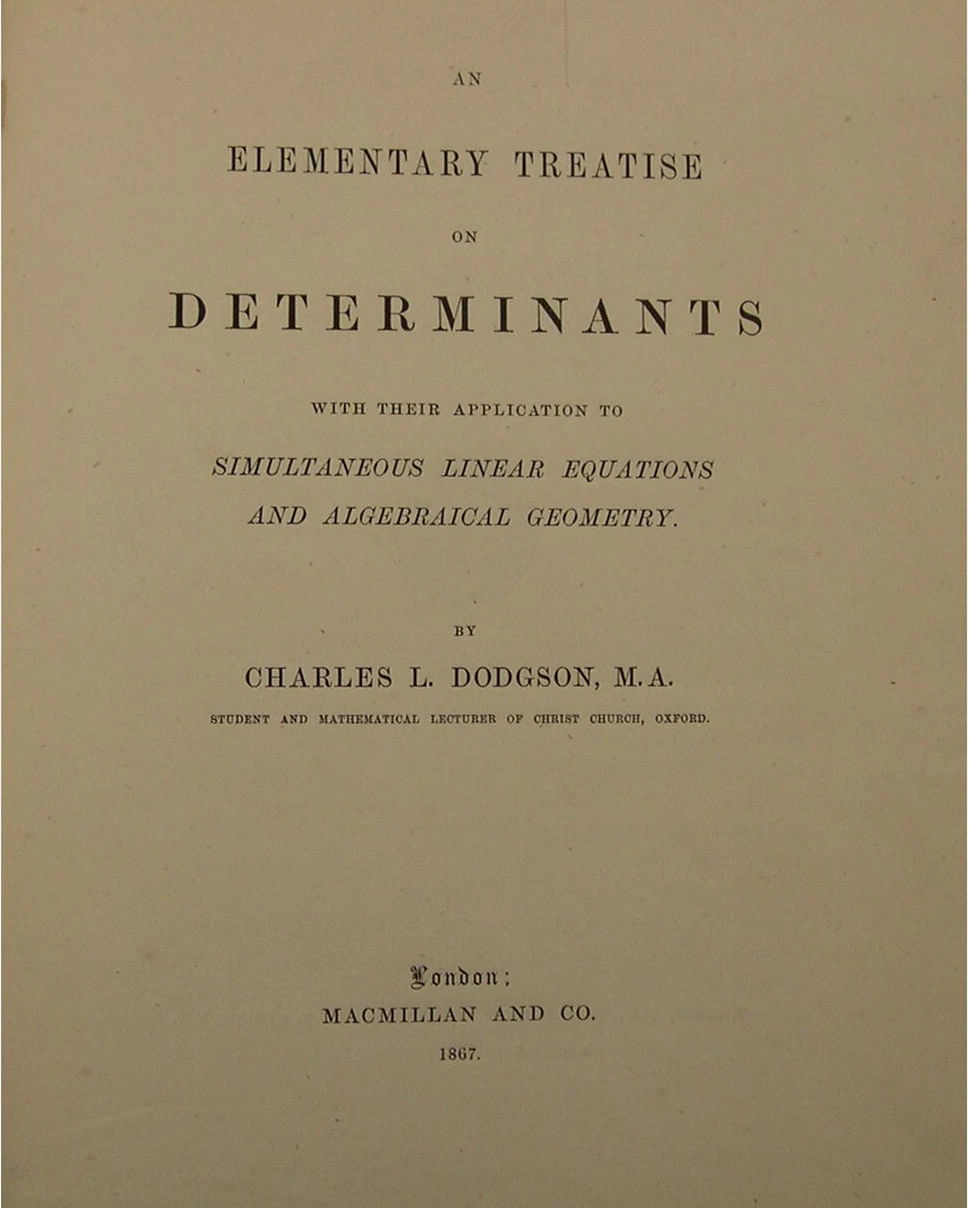
\includegraphics[width= 1\linewidth]{3}
		\caption{\small\textit{\color{quantoan}Hình $3$. The title page of Dodgson’s Elementary Treatise on Determinants, $1867$ (from the Wakeling Collection)}}
		\vspace*{-10pt}
	\end{figure}
	Khi \textit{Chuyên luận về định thức} ra mắt, có lẽ chỉ có một nhóm nhỏ độc giả có đặc quyền mới biết được bí mật nhỏ của tác giả, và ``nó là một phát hiện hoàn toàn bất ngờ với những sinh viên đại học lần đầu tiên được biết rằng ông Dodgson của trường Christ Church và Lewis Carroll chính là một" (Colingwood $1898$, tr.$110$). Một trong những người viết đánh giá về chuyên luận dường như biết điều đó, vì ông ta kết thúc bài đánh giá của mình bằng cách hy vọng ``có thêm khảo sát về thế giới thần tiên đại số tùy chọn [của tác giả]". Sự ám chỉ này đến truyện \textit{Alice} chắc hẳn đã khiến Dodgson khó chịu, một người đã rất cố gắng giữ bí mật về danh tính của mình. Dodgson phàn nàn trong một bức thư gửi cho chị dâu của mình, vào ngày $31$ tháng $7$ năm $1890$, rằng ông thấy khá kỳ lạ rằng ``mọi người sẽ không hiểu rằng, khi một tác giả sử dụng \textit{bút danh}, thì mục đích là \textit{tránh} việc công khai danh tính cá nhân, điều mà họ luôn cố gắng thúc giục anh ta". Có vẻ như việc Dodgson nhất quyết giữ bí mật danh tính của mình chỉ khiến những ``kẻ săn đuổi" ông trở nên đông đảo và quyết tâm hơn. Quả là tình huống đó hẳn đã gợi nên sự tò mò và hấp dẫn, và dễ dàng hình dung được sự ngạc nhiên của một độc giả nhiệt tình của \textit{Alice}, không biết rằng tác giả của nó là một giảng viên toán tại Oxford, khi đối diện với cuốn sách tiếp theo của tác giả, về chủ đề định thức, và được cho biết tác giả thực sự là ai. Những gì đã có thể là một giai thoại thú vị đã trở thành một câu chuyện lan truyền chóng mặt khi độc giả bối rối tình cờ lại chính là nữ hoàng.
	\vskip 0.1cm
	Câu chuyện này quá hay và không khó để có thể là sự thật. Thực sự là nữ hoàng biết, và có thể rất thích truyện \textit{Alice}. Bà  chỉ cần hỏi, và có thể bà ấy đã hỏi, về cuốn sách tiếp theo của tác giả, để khiến cho \textit{câu chuyện} xảy ra. Đó là một \textit{câu chuyện} tuyệt vời, và sẽ còn tuyệt vời hơn nếu Dodgson không hoàn toàn phủ nhận nó, gần ba mươi năm sau thời điểm mà nó được cho là đã xảy ra.
	\vskip 0.1cm
	\textbf{\color{quantoan}Phủ nhận} 
	\vskip 0.1cm
	Đến năm $1896$, Dodgson là một tác giả nổi tiếng từ chối tận hưởng danh tiếng của mình. Phần tiếp theo của câu chuyện, \textit{Đi qua tấm gương}, cũng  thành công như truyện \textit{Alice ở xứ sở diệu kỳ}.
	\vskip 0.1cm
	Sau đó, ông xuất bản nhiều tác phẩm hư cấu khác, nhưng không có tác phẩm nào thực sự sánh được với hai truyện \textit{Alice}. Là một nhà toán học, ông cũng đã xuất bản nhiều về nhiều chủ đề khác nhau, đặc biệt là bảo vệ một cách đẹp đẽ hình học Euclid trước những sách giáo khoa mới muốn thay thế nó trong các trường trung học và đại học. Trong những năm cuối đời, ông viết một chuyên luận về logic nhằm giúp chủ đề này có thể tiếp cận tới một công chúng rộng rãi. Không giống như các đồng nghiệp của mình tại Đại học Oxford, Dodgson đã chấp nhận lý thuyết logic hình thức mới được phát triển ở Anh bởi George Boole và những người theo trường phái của ông. Phần đầu tiên của chuyên luận của Dodgson, \textit{Logic hình thức}, xuất bản vào tháng $2$ năm $1896$. Lần tái bản thứ nhất, ra mắt vào đầu tháng $6$ cùng năm, có lời tựa được đề ngày $11$ tháng $5$ năm $1896$ (Hình $4$). Ngoài một vài thay đổi và sửa chữa nhỏ, nó có một phần tái bút sau trang tiêu đề, với ghi chú sau:
	\vskip 0.1cm
	\textit{Tôi xin nhân cơ hội này để phủ nhận một cách công khai nhất  có thể  một câu chuyện ngớ ngẩn, được lan truyền trên báo chí, về việc tôi đã tặng một số cuốn sách nào đó cho Nữ hoàng. Nó được lặp đi lặp lại liên tục, và là thêu dệt hoàn toàn, đến nỗi tôi nghĩ rằng đáng để tuyên bố, một lần dứt điểm, rằng nó tuyệt đối sai trong mọi chi tiết: không có bất kỳ điều gì thậm chí hơi giống như thế đã từng xảy ra cả.}
	\vskip 0.1cm
	Dodgson đã giữ ghi chú này trong lần tái bản thứ hai của cuốn sách, có lời tựa đề ngày $20$ tháng $7$ năm $1896$, nhưng vì lý do nào đó đã bỏ nó khỏi lần tái bản thứ ba, xuất bản vào đầu năm $1897$ nhưng có lời tựa vào Giáng sinh năm $1896$.
	\vskip 0.1cm
	Trong ghi chú này, Dodgson đã mạnh mẽ phủ nhận một ``câu chuyện ngớ ngẩn" về việc ông đã tặng một số cuốn sách cho nữ hoàng. Có thể lưu ý rằng giải thích của Dodgson là rất ít ỏi và có thể đề cập đến một sự việc khác, nhưng có vẻ như chỉ đơn giản là ông không muốn kể chi tiết về giai thoại để không quảng bá thêm về nó. Dodgson rõ ràng không thấy thích thú gì với \textit{câu chuyện}. Vì tin đồn đề cập đến các sự kiện được cho là diễn ra vào năm $1867$, một số tác giả tự hỏi tại sao Dodgson phải mất gần ba mươi năm để phủ nhận nó (Wakeling $2015$, tr. $315$). Derek Hudson cho rằng Dodgson có thể đã dùng thời gian này để tranh luận ``với chính bản thân mình liệu có đúng khi phản bác câu chuyện hay không (Hudson $1976$,  tr.$133$). Một lời giải thích hợp lý hơn có thể là Dodgson chỉ đơn giản là phủ nhận câu chuyện khi nó được lan truyền rộng ra, vì không có lý do gì để cho rằng tin đồn được bắt đầu trong cùng thời kỳ mà những sự việc được kể lại trong \textit{câu chuyện} được cho là đã xảy ra.
	\begin{figure}[H]
		\vspace*{-5pt}
		\centering
		\captionsetup{labelformat= empty, justification=centering}
		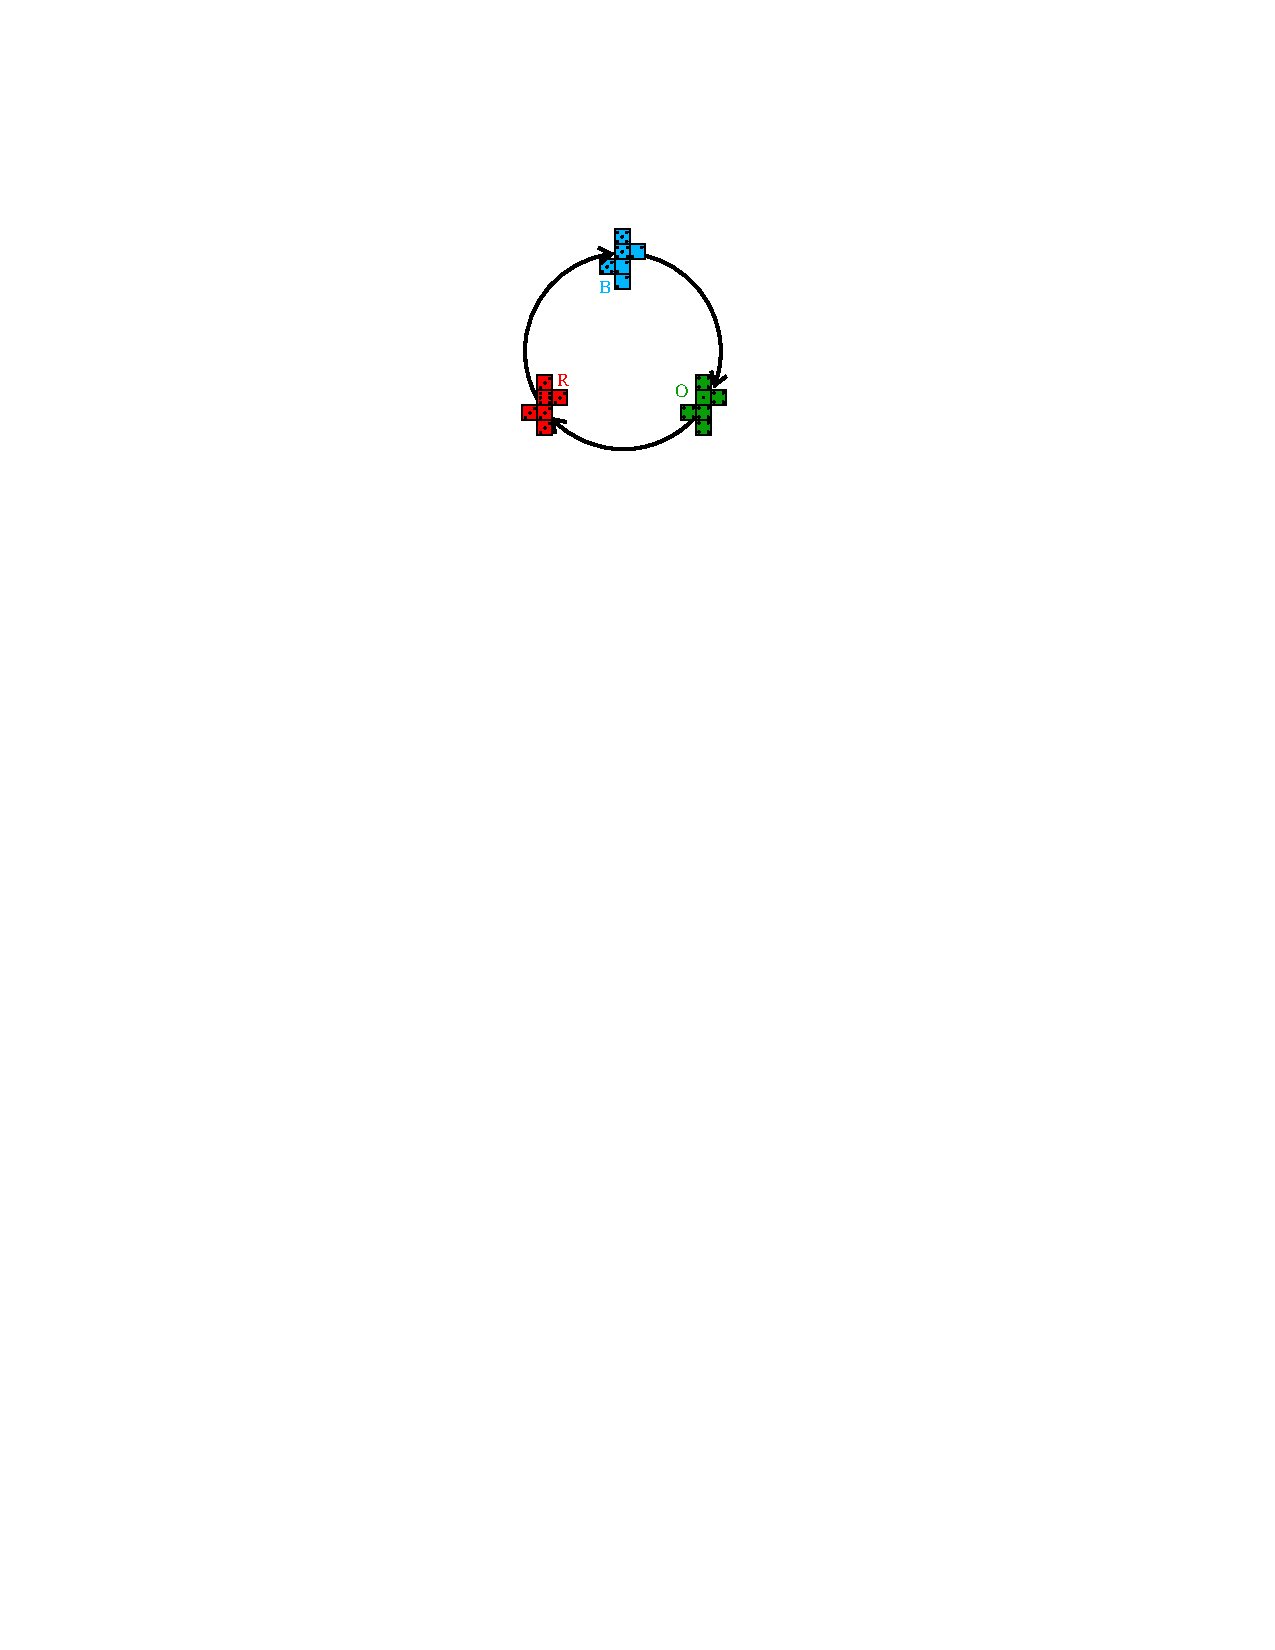
\includegraphics[width= 1\linewidth]{4}
		\caption{\small\textit{\color{quantoan}Hình $4$. The title page of Dodgson’s Symbolic Logic, second edition, $1896$, and the Advertisement page, which includes a denial of the story (from the Wakeling Collection).}}
		\vspace*{-10pt}
	\end{figure}
	Trên thực tế, có vẻ như không biết tin đồn đã bắt đầu từ khi nào. Trong một thời gian dài, người ta thậm chí đã nghĩ rằng không có bằng chứng văn bản nào về sự tồn tại của tin đồn trước sự phủ nhận của chính Dodgson vào năm $1896$. Tuy nhiên, trong những năm gần đây, một số bài báo trước đó về nó đã được tìm thấy, và giờ đây mọi thứ trở nên rõ ràng rằng tin đồn đã lan truyền khá rộng vào quãng thời gian mà Dodgson phủ nhận nó. Tin đồn chắc chắn tồn tại ít nhất từ năm $1892$, vì nó được tìm thấy trên một số tờ báo thời đó, chẳng hạn như \textit{Sporting Times}. Nó dường như đã được lan truyền rộng rãi hơn sau năm $1895$, đặc biệt là sau khi nó được Ethel Mackenzie McKenna kể lại trong số tháng $8$ năm $1895$ của \textit{Tạp chí Ladies’ Home}:
	\vskip 0.1cm
	``Trong thời kỳ  mới mẻ của sự thành công rực rỡ, ``Alice" nằm  trên tay của mọi người và những chuyến phiêu lưu vào thế giới thần tiên của cô là niềm vui thích của  người lớn cũng như trẻ em. Nữ hoàng Victoria đã gửi một thông điệp đến tác giả, xin ông gửi cho bà cuốn sách tiếp theo của mình. Giống như tất cả các thần dân của mình, bà nóng lòng muốn nghe nhiều hơn về đứa trẻ thú vị, mà nguyên mẫu là con gái của hiệu trưởng của trường Christ Church. Bà đã rất kinh ngạc khi không lâu sau đó nhận được một cuốn ``\textit{Chuyên luận về định thức}" của C. L. Dodgson, vì khi đó, ông vẫn giữ bí mật về danh tính của mình, và Nữ hoàng, cũng như cả thế giới, đã tin rằng ông chỉ đơn thuần là một người hài hước."
	\vskip 0.1cm
	Tạp chí của Mỹ này có lượng độc giả rộng lớn và ngày càng tăng vào thời Dodgson, và vào năm $1904$, nó trở thành tạp chí đầu tiên đạt được số lượng một triệu người đặt báo. Lời kể của McKenna về \textit{câu chuyện} được đăng lại trên các tạp chí khác của Mỹ, nhất là trong các mục tin đồn, tin vắn và tin tức văn học. \textit{Câu chuyện} hẳn cũng đã lan tới một số tờ báo của Anh, vì nó được đăng trên tờ \textit{Newcastle Weekly Courant}. Đúng là \textit{câu chuyện} không được tìm thấy trên các tờ báo lớn của Anh, một sự thật có thể được giải thích là do họ không muốn xuất bản những bài viết tiết lộ danh tính của Dodgson. Được biết, Dodgson không hài lòng với những bài viết như vậy và đã liên tục viết thư phàn nàn đến những tạp chí và nhà xuất bản của Anh đã tiết lộ hoặc muốn tiết lộ tên thật đằng sau bút danh của ông. Các tạp chí nước ngoài hiển nhiên nằm ngoài tầm ảnh hưởng của Dodgson, như ông thừa nhận trong một bức thư gửi cho Falconer Madan vào ngày $8$ tháng $12$ năm $1880$: ``Tôi e rằng các ấn phẩm của Mỹ nằm ngoài tầm khiếu nại của các nhà văn Anh: chỉ ở Anh, người ta mới có thể hy vọng ngăn tên mình được công bố."
	\vskip 0.1cm
	Vào năm $1895$, \textit{câu chuyện} rõ ràng là đã ``lan truyền trên báo chí" và được ``lặp đi lặp lại liên tục", như Dodgson đã viết trong lời phủ nhận của mình. Người ta lập luận rằng ``không chắc Dodgson đã xem tạp chí [\textit{Tạp chí Ladies’ Home}] này" (Wakeling $2005$, tr. $257$); tuy nhiên, ông có thể đã thấy một trích dẫn về nó được đăng lại trên các tờ báo của Anh. Chúng ta cũng biết rằng Edward Bok, chủ bút của \textit{Tạp chí Ladies’ Home}, đã đến thăm Dodgson ở Oxford để thuyết phục ông đóng góp bài cho tạp chí. Chuyến thăm này được ghi lại trong tự truyện của Bok, nhưng ngày tháng không được nêu rõ ràng. Tuy nhiên, lời kể đó gợi ý rằng nó trùng hợp với lần Bok đến thăm Rudyard Kipling, người đã được thuyết phục đóng góp câu chuyện ``William the Conqueror" của mình cho tạp chí. Do câu chuyện của Kipling xuất bản vào cuối năm $1895$, sẽ khá hợp lý khi cho rằng chuyến thăm diễn ra trước đó. Điều thú vị là Bok kể về việc ông đã hỏi Dodgson về câu chuyện gửi tặng cuốn sách \textit{Chuyên luận về định thức} cho nữ hoàng, một câu hỏi mà Dodgson  không bình luận, nhưng ``khuôn mặt của ông ấy hoàn toàn không có biểu hiện gì ngoài vẻ trắc ẩn nhằm nói với người chủ bút rằng ông ta đang mắc một sai lầm khủng khiếp" (Bok $1920$, tr. $222-223$). Trước sự thất vọng lớn của Bok, Dodgson chỉ đơn giản  phủ nhận việc mình là tác giả của hai cuốn sách \textit{Alice}. Nếu lời kể của Bok là sự thật, ông ta đã sớm được chứng kiến Dodgson bác bỏ câu chuyện, trước khi ông phủ nhận bằng văn bản, trong cuốn sách. Nhưng chúng ta có nên tin Dodgson không?
	\vskip 0.1cm
	\textbf{\color{quantoan}Liệu rằng nó đã xảy ra?}
	\vskip 0.1cm
	Việc tìm hiểu sự thật về \textit{câu chuyện} có vẻ là việc làm kỳ quái và thiếu tôn trọng bởi vì Dodgson đã phủ nhận nó một cách rõ ràng. Tuy nhiên, chúng ta không được quên rằng Dodgson thường xuyên phủ nhận (một cách không đúng) rằng ông là tác giả của  \textit{Alice}, vì vậy chúng ta không có thêm lý do gì để tin vào sự thật của lời phủ nhận này so với tất cả những lời phủ nhận khác mà chúng ta biết là không đúng. Câu chuyện của chúng ta kết nối tác giả của \textit{Alice} với tác giả của \textit{Chuyên luận về định thức}. Dodgson không có lựa chọn nào khác ngoài việc phủ nhận nó, bất kể sự thật là gì, nếu ông ấy muốn -- và chúng ta biết rằng ông thực sự muốn -- giữ bí mật về danh tính của mình.
	\vskip 0.1cm
	Chúng ta hầu như không thể nhấn mạnh đủ mức độ quan trọng của việc giữ kín danh tính đối với Dodgson. Các tiểu sử về ông chứa nhiều mẩu chuyện về việc ông từ chối là tác giả của truyện \textit{Alice} khi được hỏi về nó. Dodgson cũng từ chối lời mời tham dự các buổi chiêu đãi do nhà xuất bản của ông tổ chức, nơi ``hầu như không thể giữ được sự ẩn danh". Khi những lá thư được gửi đến trường Christ Church cho ông dưới cái tên Lewis Carroll , ông  đã gửi trả lại chúng mà không mở. Năm $1890$, ông thậm chí còn ban hành một thông cáo để gửi cho những người đã gửi thư đến như sau:
	\vskip 0.1cm
	``Ông Dodgson thường xuyên bị những người lạ gửi thư đến với giả định khá trái phép rằng ông tuyên bố, hoặc trong một chừng mực nào đó thừa nhận quyền tác giả của những cuốn sách không được xuất bản dưới tên ông, đến mức ông thấy cần phải tuyên bố điều này, một lần dứt điểm, như một câu trả lời cho tất cả các bức thư như vậy. Ông ta không tuyên bố hay thừa nhận bất kỳ mối liên hệ nào với bất kỳ bút danh nào, hoặc với bất kỳ cuốn sách nào không được xuất bản dưới tên của chính ông ta. Do đó, không có quyền giữ lại, hoặc thậm chí đọc thư bên trong, ông ta gửi trả lại nó cho người viết thư đã viết sai địa chỉ."
	\vskip 0.1cm
	Lưu ý rằng Dodgson không chính thức phủ nhận là tác giả của các truyệnAlice trong thông cáo này; ông chỉ đơn thuần từ chối việc đòi hoặc thừa nhận quyền tác giả đó. Nhưng Lloyd Humberstone khuyến cáo một cách đúng đắn rằng
	``Chúng ta không nên coi trọng những lời phủ nhận [của Dodgson] hơn những lời phủ nhận của một nghi phạm bị bắt trong cuộc truy tìm Jack the Ripper của cảnh sát, người khẳng định rằng anh ta không muốn được biết đến với cái tên đó, rằng anh ta không tuyên bố -- hay thừa nhận -- đã thực hiện bất kỳ vụ giết người nào, v.v." (Humberstone $1995$, tr. $498$).
	\vskip 0.1cm
	Đúng là bí mật về danh tính của Dodgson dần dần được hé lộ và có lẽ nó đã trở thành một bí mật công khai vào những năm cuối đời của ông. Các tờ báo thỉnh thoảng có đề cập đến danh tính của ông, và từ điển các bút danh thường liệt kê ông. Khá hợp lý khi cho rằng bí mật có lẽ được lan truyền qua số đông bạn bè và người quen của ông. Tuy nhiên, Dodgson vẫn từ chối thừa nhận là tác giả của những truyện \textit{Alice} khi những người lạ tiếp cận ông hoặc viết thư cho ông về nó. Những nỗ lực nhiệt thành của Dodgson để bảo vệ bí mật của mình,  thậm chí ngay cả sau này khi danh tính của ông đã được biết đến rộng rãi, hẳn đã khiến những người cùng thời của ông phải tò mò. Các cuốn tiểu sử về ông thuật lại cái cách mà trong suốt cuộc đời của mình, ông ấy là ``\textit{mục tiêu thường xuyên của những lời đồn đại}".
	\vskip 0.1cm
	Việc phủ nhận \textit{câu chuyện} của Dodgson cần phải được hiểu trong bối cảnh này: \textit{câu chuyện} chỉ là một trong số rất nhiều tin đồn về tác giả của \textit{Alice} và sự phủ nhận chỉ là một trong số rất nhiều tình huống mà Dodgson cố gắng giữ bí mật danh tính của mình. Tuy nhiên, có một nét nổi bật về việc Dodgson phủ nhận \textit{câu chuyện} trong cuốn \textit{Logic Hình thức} của ông. Dodgson tin tưởng vào lợi ích xã hội của logic hình thức và muốn cuốn sách của mình dễ tiếp cận đối với rộng rãi độc giả. Để quảng bá rộng rãi hơn cho cuốn sách chuyên luận  của mình, ông đã dùng bút danh văn học của mình thay vì tên thật, vốn thường được sử dụng cho các công trình toán học. Vì vậy, lời phủ nhận mà ông  đưa vào chuyên luận có thể là dịp duy nhất mà Dodgson, dưới cái tên Lewis Carroll, phủ nhận mối liên hệ của ông với Charles L. Dodgson.
	\vskip 0.1cm
	Chúng tôi đã nói ở trên rằng \textit{câu chuyện} thực sự không khó để có thể là  thật. Thật vậy, có những lý do chính đáng để tin rằng \textit{câu chuyện} đã thực sự xảy ra, và người ta sẽ không ngạc nhiên nếu nó đã xảy ra. Tuy nhiên, Thomas B. Strong, một người bạn của Dodgson, trong hồi ký viết năm $1932$, đưa ra hai lý do để không tin vào điều đó:
	\vskip 0.1cm
	``Thật trái ngược với toàn bộ thái độ của Dodgson đối với Hoàng gia và với cung cách đúng mực của ông ấy nếu  ông ấy giễu cợt Nữ hoàng như vậy. Và nó hoàn toàn trái ngược với thái độ của ông ấy đối với những cuốn sách của mình. Ông ấy luôn từ chối thừa nhận với bất kỳ người nào, ngoại trừ một số những người có đặc quyền đặc biệt, rằng ông ấy là Lewis Carroll."
	\vskip 0.1cm
	Có vẻ như Strong không nhận thấy rằng hai lý do ông ấy đưa ra có phần trái ngược nhau. Thật vậy, Dodgson hoặc phải gửi cuốn sách tiếp theo của mình, và do đó tiết lộ danh tính của ông, hoặc từ chối gửi nó, và do đó từ chối yêu cầu của nữ hoàng, mặc dù ông có thể đã  lập luận rằng cuốn sách tiếp theo của Lewis Carroll hoàn toàn không phải là cuốn sách tiếp theo của Charles Dodgson.
	\vskip 0.1cm
	Lưu ý rằng lý do đầu tiên mà Strong đưa ra cho thấy rằng việc Dodgson gửi tặng một cuốn sách toán cho nữ hoàng là điều đáng hổ thẹn và thô lỗ. Nhưng lý do thứ hai có vẻ như không đúng, vì chúng ta có thể tưởng tượng Dodgson hẳn sẽ vui vẻ coi nữ hoàng là một trong số ``những người có đặc quyền" được ông đã tiết lộ danh tính của mình, và chắc chắn ông đã tiết lộ điều đó để được giao thiệp với một số nhân vật nổi tiếng cùng thời.
	\vskip 0.1cm
	Dodgson không đáng tin cậy lắm khi ông phủ nhận những \textit{câu chuyện} tiết lộ danh tính của mình; thậm chí chỉ cần nhìn qua danh sách những phủ nhận của ông là đủ để ủng hộ việc không tin vào ông. Nhưng có thể có một lý do chính đáng để tin Dodgson một lần. Thật vậy, việc Dodgson phủ nhận \textit{câu chuyện} sẽ không ảnh hưởng đến niềm tin của chúng ta về nó nếu nhân vật liên quan không phải là nữ hoàng. Tôi không tin rằng việc tặng một cuốn sách toán học cho nữ hoàng sẽ đi ngược lại cách hành xử đúng mực của Dodgson. Tuy nhiên, việc công khai phủ nhận một câu chuyện liên quan đến nữ hoàng, câu chuyện có thể sẽ được nữ hoàng công nhận là thật, có thể sẽ bị coi là đáng hổ thẹn đối với một thần dân thời Victoria, một người ``yêu nước nồng nàn và là một tín đồ trung thành của những hoạt động của hoàng gia" (Hudson $1976$, $133$).
	\vskip 0.1cm
	Được biết, Dodgson rất kính trọng nữ hoàng và hoàng gia. Trong suốt cuộc đời mình, ông đã có một số dịp gặp gỡ các thành viên của hoàng gia, và ông chắc chắn đã quen với một số người trong họ. Ông đã tường thuật chi tiếttrong nhật ký của mình chuyến thăm trường Christ Church của nữ hoàng, vào tháng $12$ năm $1860$. Trong các chuyến thăm Oxford của các thành viên hoàng gia, ông tìm cách được giới thiệt để chụp ảnh họ. Dodgson là một nhiếp ảnh gia có tiếng, được nhiều nhân vật nổi tiếng cùng thời làm mẫu. Đáng chú ý, ông đã chụp được ảnh Hoàng tử Frederick của Đan Mạch vào năm 1863 và Hoàng tử Leopold (con trai út của nữ hoàng) vào năm 1875. Theo Collingwood, một số bức ảnh của  Dodgson ``đã được nữ hoàng xem, và bà nói rằng rất thích chúng"  (Collingwood $1898$, tr. $102-104$).
	\vskip 0.1cm
	Đúng là trong thư từ cá nhân của mình, Dodgson đã bịa ra một số câu chuyện liên quan đến nữ hoàng để mua vui cho các bạn thư của ông. Một lần, ông đã ``soạn một bức thư giả của nữ hoàng Victoria mời mình đến một bữa tiệc trong vườn". Một lần khác, ông giả vờ rằng nữ hoàng đã hỏi xin ông một bức ảnh, nhưng ông từ chối vì ``nguyên tắc của ông là không bao giờ cho ảnh của mình, ngoại trừ cho những cô gái \textit{trẻ}" (Cohen và Green $1979$, tr. $135-136$ và $116$). Edward Wakeling đã nhận xét tinh tế rằng ``đó dĩ nhiên chính là cách mà những câu chuyện và tin đồn bắt đầu" (Wakeling $2015$, tr. $316$). Vì vậy, có thể \textit{câu chuyện} của chúng ta cũng được bắt đầu bởi chính Dodgson, để đùa vui một số người bạn gần gũi, trước khi trò đùa trở thành một tin đồn không thể ngăn chặn.
	\vskip 0.1cm
	\textbf{\color{quantoan}Tác giả của \textit{Alice}}
	\vskip 0.1cm
	Đương nhiên, sự phủ nhận của Dodgson về \textit{câu chuyện} vào năm $1896$ không làm nó ngừng lan truyền. Ví dụ, nó được tìm thấy vào năm sau đó trong mục về Dodgson trong cuốn sách đầy tham vọng \textit{Thư viện về Văn học hay nhất thế giới}, trong đó chủ biên nhận xét rằng 
	\vskip 0.1cm
	``hiếm khi một bộ óc kép như vậy -- khi thì viết những điều hoàn toàn ngớ ngẩn và rất dí dỏm, khi thì lại khám phá những điều phức tạp của toán học cao cấp -- lại có một thể hiện kỳ lạ hơn (Warner $1897$, tr. $309$).
	\vskip 0.1cm
	\textit{Câu chuyện} cũng được tìm thấy vào năm $1897$ trong chuyên mục tin ngắn của tờ \textit{Northern Echo}, kèm theo một số câu thơ lấy cảm hứng từ đó.
	\vskip 0.1cm
	Kể từ đó, \textit{câu chuyện} được kể thường xuyên đến mức có đến mấy bản khác nhau của nó. Một số phiên bản cho rằng Dodgson đã gửi cho nữ hoàng cả một bộ sách chứ không chỉ là cuốn \textit{Chuyên luận về định thức}. Một số phiên bản khác cho rằng thực ra người bán sách của nữ hoàng mới là người được yêu cầu giao sách của Dodgson cho nữ hoàng. Bất chấp sự khác biệt của chúng, tất cả các lời kể đều thống nhất ở một điểm trọng tâm: nữ hoàng đã yêu cầu một tác phẩm khác của tác giả của một câu chuyện thiếu nhi và thật ngạc nhiên, bà đã nhận được một cuốn sách toán.
	\vskip 0.1cm
	Không khó để hiểu được sự thành công của ``giai thoại hấp dẫn không chịu phai nhạt, mặc dù nó khá sai sự thật" này (Hudson $1976$, tr. $132$). ``Riêng việc nó trùng khớp quá mức với hình ảnh phổ biến" về tính cách kép đã đủ giải thích cho sự dai dẳng của nó (Heath $1974$, tr.$3$). Từ lâu, công việc chính của các nhà viết tiểu sử của Dodgson là giải quyết điều mà họ coi là một nghịch lý: ``Bằng cách nào mà Lewis Carroll, một nhà toán học  khó tính, dè dặt và sùng đạo sâu sắc thời Victoria, lại có thể tạo ra những câu chuyện đã trở thành những tác phẩm thiếu nhi kinh điển được yêu thích nhất trong văn học Anh?" (Cohen $1995$, tr. $19$).
	\vskip 0.1cm
	Nhiều nhà nghiên cứu đã cố gắng giải quyết bí ẩn này và chứng minh sự thống nhất (hoặc ít nhất là sự tương đồng) giữa hai mặt của  thiên tài của Dodgson. Một số người đã diễn giải quá mức các câu chuyện Alice nhằm tìm kiếm những chân lý toán học ẩn náu mà chỉ một nhà toán học mới có thể lồng vào đó. Một số người khác đã phóng đại phần toán học giải trí của Dodgson mà chỉ một nhà văn hài hước mới có thể tạo ra. Nhưng từ lâu, chiến lược chính của các người theo chủ nghĩa Carroll là làm cho cái tên Dodgson trở nên mờ nhạt, chìm về phía sau vì cho rằng ``những công trình của Charles Dodgson kém thú vị hơn những tác phẩm của Lewis Carroll".
	\vskip 0.1cm
	Việc hạ thấp Dodgson để ủng hộ Carroll đã bắt đầu từ khi Dodgson còn sống. Ví dụ, một người viết nhận xét về cuốn sách \textit{Pillow--Problems} của Dodgson, một tập hợp các bài toán mà ông ký bằng tên thật của mình, đã bày tỏ một cách rõ ràng thị hiếu của mình: 
	\vskip 0.1cm
	``Và, sau cùng, thế giới cần Lewis Carroll, người một mình hiểu được ``trí thông minh siêu hình" của trẻ nhỏ, và tức thì đưa người lớn tuổi nhất trong chúng ta đi dạo qua vùng đất mơ ước của chúng, hơn là ông Dodgson, người không có vẻ gì là một người du hành trong biển sâu của tư tưởng (Newton, Kelvin là vậy) mà chỉ là một nhà toán học tao nhã."
	\vskip 0.1cm
	Ngoài sự bực bội khi thấy danh tính của mình bị tiết lộ, người ta có thể tưởng tượng được Dodgson có thể đã cảm thấy khó chịu như thế nào khi danh tiếng văn học can thiệp vào việc đánh giá các công trình toán học của ông. Tuy nhiên, sự cám dỗ của việc liên kết hai cái tên là rất mạnh, và nhiều đồng nghiệp làm toán của Dodgson chắc chắn đã không cưỡng lại được. Ví dụ, Hugh MacColl, người đã đã viết nhận xét về một số cuốn sách toán của Dodgson trong tạp chí \textit{Athenaeum} đã đề cử cuốn sách \textit{Lý thuyết mới của sự song song} của Dodgson, mà ông thấy ``cũng thú vị như những điều kỳ lạ cô bé Alice đã gặp ở xứ sở diệu kỳ". Một ví dụ khác xảy ra vào năm $1894$, khi một bài toán  logic do Dodgson nghĩ ra được lưu truyền giữa các nhà logic học người Anh. John Venn muốn thảo luận về nó trên báo in và xin phép Dodgson. Ông đồng ý nhưng yêu cầu Venn ``không được đề cập với bất kỳ ai  \textit{tên thật} [của ông], một cách có liên quan đến bút danh [của ông]". Venn hẳn đã rất bối rối, vì ông đã không đề cập đến cả hai cái tên trong cuốn sách của mình, mà chỉ gọi bài toán logic đang được thảo luận là Bài toán Alice, ``người đề xuất nó, đối với độc giả nói chung, được biết đến nhiều hơn trong một nhánh văn học rất khác."
	\vskip 0.1cm
	Tình hình sau đó không có nhiều thay đổi. Trong cuốn \textit{Cơ sở về Lịch sử toán} học, Nicolas Bourbaki gọi \textit{Chuyên luận về định thức} của Dodgson  là  ``một cuốn sách khó hiểu, với sự cẩn thận và tỉ mỉ đặc trưng của ông,  tác giả nổi tiếng của \textit{Alice ở xứ sở diệu kỳ}"  mà không nêu tên tác giả của nó; chỉ cần biết rằng chuyên luận được viết bởi tác giả của \textit{Alice}. Sự nổi tiếng ngày nay của Dodgson trong giới toán học chắc chắn đã được hưởng lợi từ vị thế văn học của ông. Ngày nay, có một nhánh nghiên cứu đáng nể chuyên về Dodgson trong cộng đồng các nhà sử học toán học, không như nhiều đồng nghiệp đã bị lãng quên của ông. Dodgson có lẽ sẽ không bao giờ thiếu độc giả, nhưng ông luôn đối mặt với nguy cơ không được đọc một cách nghiêm túc. Độc giả hiện đại của Dodgson biết rằng họ đang đọc ``tác giả của Alice." Thật vậy, có lẽ  phần lớn độc giả của Dodgson đọc sách của ông chính là vì họ biết ông là tác giả của \textit{Alice}. Như vậy, họ thường mong gặp những điều huyền ảo ở những nơi không có nhiều, và khi không có nhiều, đôi khi họ thêm thắt một chút.
	\vskip 0.1cm
	Thật là xấu hổ cho nữ hoàng nếu bài viết này kết thúc mà không có một vài lời về cách bà được miêu tả trong \textit{câu chuyện}. Mọi người dễ dàng hiểu được sự ngạc nhiên của bà khi nhận được chuyên luận về định thức của Dodgson, nếu bà quả thựcnhận được cuốn sách, với lý do rằng ``nữ hoàng, giống như phần còn lại của thế giới,  tin rằng ông ấy chỉ đơn thuần là một người hài hước" (McKenna $1895$, tr. $8$). Bà có lẽ cũng sẽ phản ứng tương tự nếu nhận được một chuyên luận về thực vật nhiệt đới hoặc một nghiên cứu về nghệ thuật thời trung cổ, khi tất cả những gì bà mong đợi là một câu chuyện cho trẻ em. Tuy nhiên, sự đặc biệt của \textit{câu chuyện} rõ ràng nảy ra từ định kiến sáo mòn rằng toán học và văn học thuộc về các lĩnh vực tách biệt và không thể dung hòa. Nữ hoàng đã rất ngạc nhiên vì bà mong đợi tác giả là ``một người hài hước", nhưng điều khiến cho sự ngạc nhiên của bà vô cùng thú vị là nếu như bà đã kỳ vọng tác giả là bất kỳ ai khác khác ngoài ``một người hài hước", có lẽ bà sẽ không thể ngờ ông ta là một nhà toán học.
	\vskip 0.1cm
	Ngoài sự ngạc nhiên, nhiều phiên bản của \textit{câu chuyện} cho rằng nữ hoàng không hề cảm thấy thích thú. Chúng ta đã thấy một số nhà bình luận phủ nhận câu chuyện với lý do rằng việc tặng một cuốn sách như vậy là vô lễ. Nếu \textit{câu chuyện} quả thực đã xảy ra, những nhà bình luận như vậy cho rằng nữ hoàng sẽ cảm thấy bị xúc phạm. Chúng tôi không biết năng lực toán học của nữ hoàng, nhưng giả sử rằng bà không phải là một người yêu thích toán học, chúng ta vẫn thấy không có lý do gì để bà cảm thấy không hài lòng hoặc không được tôn trọng (mặc dù có thể đã thất vọng). Đầu tiên, chúng ta có thể tưởng tượng rằng nữ hoàng cảm thấy thích thú với sự cố nhỏ này, cũng như cách nó đã khiến nhiều thế hệ độc giả sau này thích thú. Và thứ hai, lời buộc tội  thiếu tôn trọng dường như tận dụng niềm tin rộng rãi rằng toán học là một thứ buồn tẻ, không phù hợp với những nghi thức xã giao, và do đó không thích hợp để làm  một món quà chân thành.
	\vskip 0.1cm
	Câu chuyện Dodgson tặng một cuốn sách toán cho nữ hoàng Victoria là một giai thoại kinh điển trong thế giới toán học. Nó bảo chúng ta rằng một tiểu thuyết gia thành công khó có thể là một nhà toán học chuyên nghiệp và các nữ hoàng có lẽ không hứng thú với những cuốn sách toán. Không cần phải xem xét nó một cách quá nghiêm túc. Nhưng  thành công của nó chắc chắn phản ánh những điều cũ rích nhưng còn mãi về toán học là gì, nhà toán học là ai, và sự sáng tạo toán học bắt nguồn từ đâu.
	\vskip 0.1cm
	\textbf{\color{quantoan}Tài liệu tham khảo} 
	\vskip 0.1cm
	[$1$]	Beale, Tony ($1973$). C. L. Dodgson: mathematician. In Denis Crutch, ed. \textit{Mr. Dodgson}, pp. $26-33$. London: The Lewis Carroll Society.
	\vskip 0.1cm
	[$2$]	Bok, Edward ($1920$). \textit{The Americanization of Edward Bok: The Autobiography of a Dutch Boy Fifty Years Later}. New York: Charles Scribner’s sons.
	\vskip 0.1cm
	[$3$]	Cohen, Morton N. ($1995$). \textit{Lewis Carroll: A Biography}. New York: Alfred A. Knopf.
	\vskip 0.1cm
	[$4$]	Cohen, Morton N., and Roger Lancelyn Green, eds. ($1979$). \textit{The Letters of Lewis Carroll}. New York: Oxford University Press.
	\vskip 0.1cm
	[$5$]	Collingwood, Stuart Dodgson ($1898$). \textit{The Life and Letters of Lewis Carroll (Rev. C. L. Dodgson)}. London: T. Fisher Unwin.
	\vskip 0.1cm
	[$6$]	Heath, Peter, ed. ($1974$). The Philosopher’s Alice. London: Academy Editions.
	\vskip 0.1cm
	[$7$]	Hudson, Derek ($1976$). \textit{Lewis Carroll: An Illustrated Biography}. London: Constable.
	\vskip 0.1cm
	[$8$]	Humberstone, Lloyd ($1995$). Names and pseudonyms. \textit{Philosophy} $70$ ($274$), $487-512$.
	\vskip 0.1cm
	[$9$]	McKenna, Ethel Mackenzie (August $1895$). The author of ``Alice in Wonderland." \textit{Ladies’ Home Journal} $8$.
	\vskip 0.1cm
	[$10$]	Wakeling, Edward, ed. ($1999$). \textit{Lewis Carroll’s Diaries: The Private Journals of Charles Lutwidge Dodgson (Lewis Carroll)}, vol. $5$. The Lewis Carroll Society, Bedfordshire: Luton Press.
	\vskip 0.1cm
	[$11$]	Wakeling, Edward, ed. ($2005$). \textit{Lewis Carroll’s Diaries: The Private Journals of Charles Lutwidge Dodgson (Lewis Carroll)}. Vol. $9$, The Lewis Carroll Society, Herefordshire: Clifford Press.
	\vskip 0.1cm
	[$12$]	Wakeling, Edward ($2015$). \textit{Lewis Carroll: The Man and His Circle}. London: I. B. Tauris.
	\vskip 0.1cm
	[$13$]	Warner Charles Dudley, ed. ($1897$). \textit{A Library of the Wold’s Best Literature: Ancient and Modern}. Vol. $8$. New York: The international Society.
\end{multicols}
%	 \newpage
%
%	 \setcounter{figure}{0}
%	 \thispagestyle{toancuabinone}
\pagestyle{toancuabi}
\everymath{\color{toancuabi}}
%\blfootnote{$^1$\color{toancuabi}...}
\graphicspath{{../toancuabi/pic1/}}
\begingroup
\AddToShipoutPicture*{\put(0,616){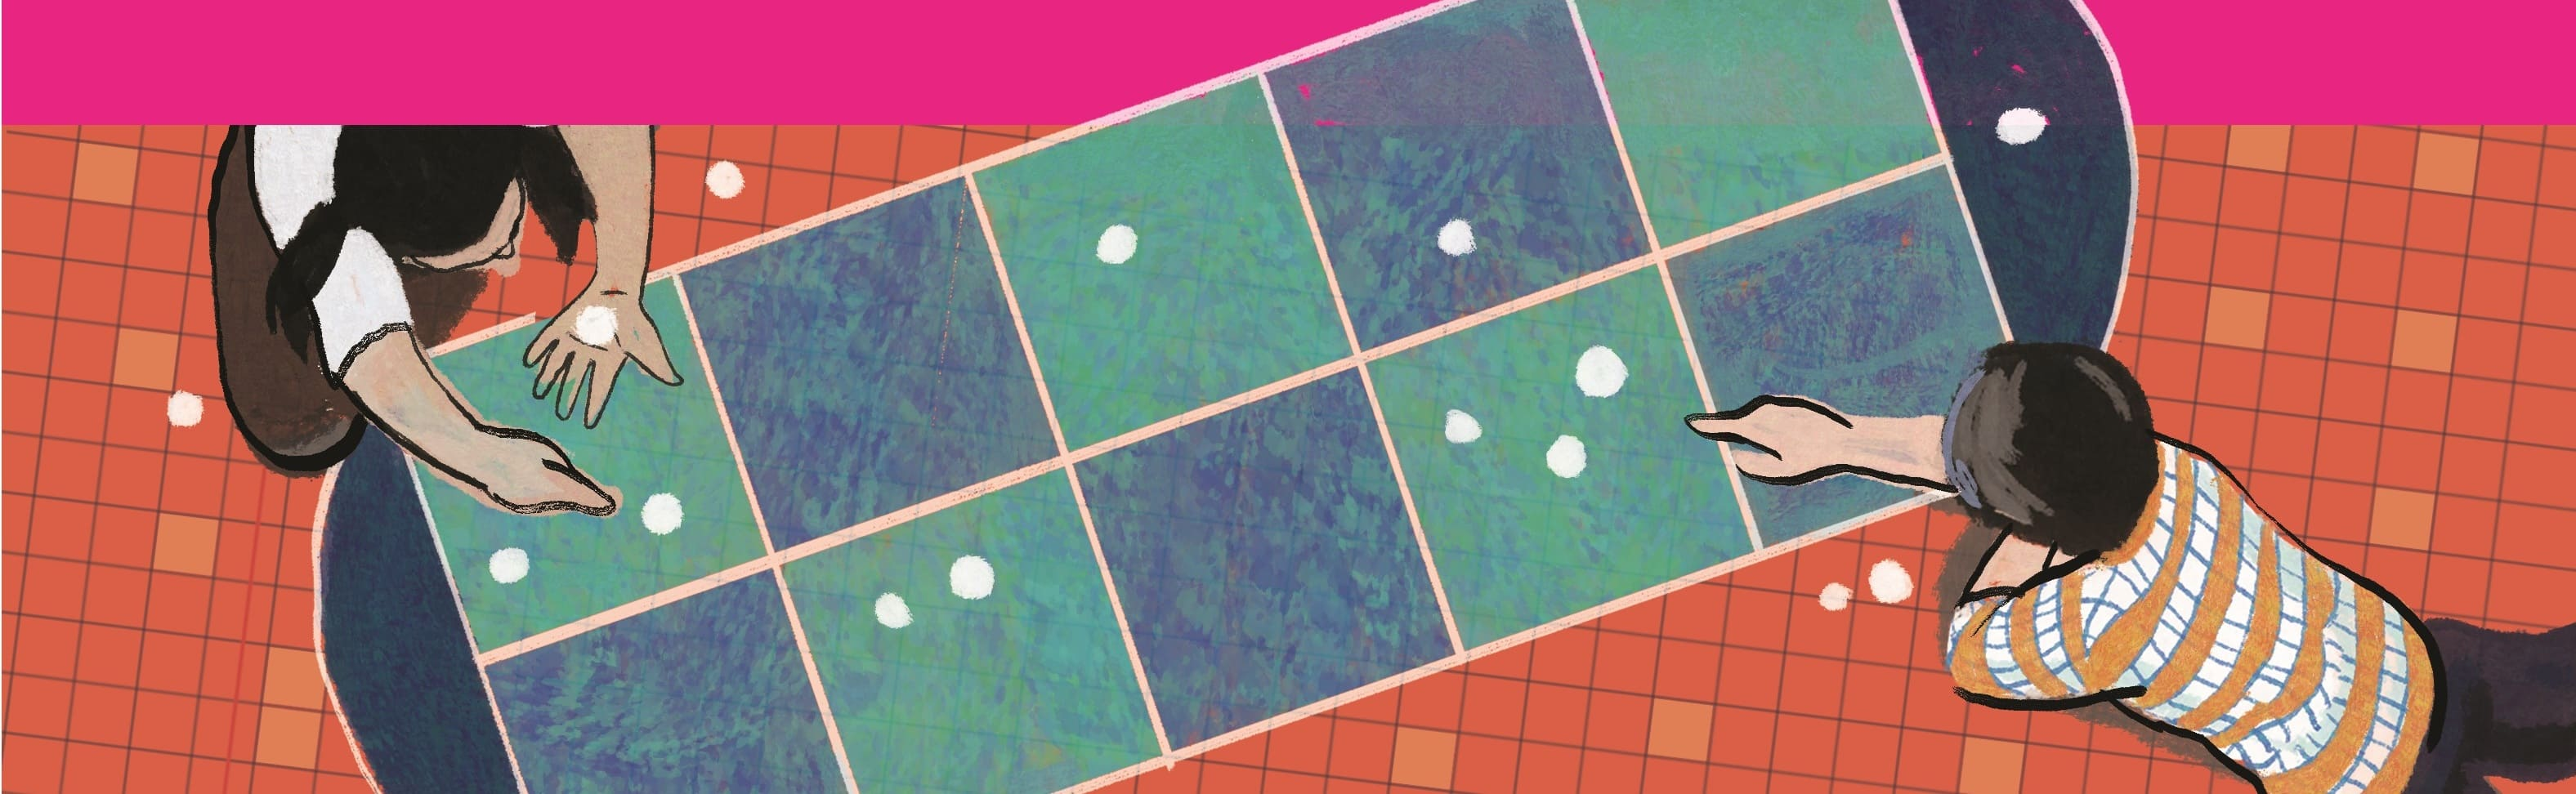
\includegraphics[width=19.3cm]{../bannertoancuabi}}}  
\AddToShipoutPicture*{\put(38,553){
\includegraphics[scale=0.95]{../tieude1.pdf}}} 
\centering
\endgroup
\vspace*{152pt}

\tikzset{
	mystyle/.style={
		below,
		yshift=-0.5cm,
		text width=1.2cm,
		align=center
	}
}

\begin{multicols}{2}
%		Mặc dù ngày nay, một số bộ lạc thổ dân sống ở rừng rậm Amazon chỉ có những từ: ``một", ``hai" và ``nhiều" để nói về số lượng hay một số bộ lạc khác chỉ đếm từ $1$ đến $5$, từ xa xưa người tiền sử đã đếm những số lớn hơn bằng cách đánh dấu lên đá hay xương động vật.
%	\vskip 0.1cm
%	\begin{figure}[H]
%		\centering
%		\vspace*{-5pt}
%		\captionsetup{labelformat= empty, justification=centering}
%		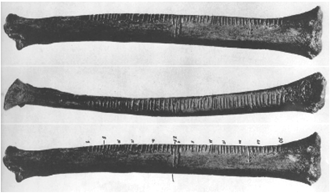
\includegraphics[width=1\linewidth]{1}
%		\caption{\textit{\color{toancuabi}Hình $1$: Những mảnh xương chó sói có các khía, được cho là ra đời cách đây $30000$ năm và là công cụ để đếm của người thời tiền~sử.}}
%		\vspace*{-10pt}
%	\end{figure}
%	Từ hàng nghìn năm trước, ở những nền văn minh khác nhau, con người đã phát minh ra những hệ thống số để phục vụ mục đích đầu tiên là ghi nhớ những đại lượng lớn. Những con số đó chính là khởi nguồn của toán học. Trong bài viết này chúng ta hãy cùng tìm hiểu về những cách ghi số của những nền văn minh khác nhau thời cổ đại nhé.
%	\begin{figure}[H]
%		\centering
%		\vspace*{-5pt}
%		\captionsetup{labelformat= empty, justification=centering}
%		\resizebox{\columnwidth}{!}{\begin{tikzpicture}[scale=0.6]
%			\draw [ fill=red] (0,0) rectangle (5,1) node[pos=.5] {\tiny TIỀN SỬ};
%			\draw [fill=quantoan] (5,0) rectangle + (4,1) node[pos=.5] {\tiny CỔ ĐẠI};
%			\draw [fill=diendantoanhoc] (9,0) rectangle + (3,1) node[pos=.5] {\tiny TRUNG ĐẠI};
%			\draw [fill=cackithi] (12,0) rectangle + (3,1) node[pos=.5] {\tiny CẬN ĐẠI};
%			\draw [fill=gocco] (15,0) rectangle + (3,1) node[pos=.5] {\tiny HIỆN ĐẠI};
%			\draw[<->, line width=1.0mm, toancuabi] (0,-0.8) -- (18,-0.8);
%			\draw[line width=1.0mm, blue] (1,-1.1) -- (1,-0.5) node[mystyle] {$2000000$ năm trước};
%			\draw[line width=1.0mm, blue] (5,-1.1) -- (5,-0.5) node[mystyle] {$5000$ năm trước};
%			\draw[line width=1.0mm, blue] (9,-1.1) -- (9,-0.5)  node[mystyle] { năm $500$};
%			\draw[line width=1.0mm, blue] (12,-1.1) -- (12,-0.5) node[mystyle] {năm $1500$};
%			\draw[line width=1.0mm, blue] (15,-1.1) -- (15,-0.5) node[mystyle] {năm $1800$};
%			\draw[line width=1.0mm, blue] (17.2,-1.1) -- (17.2,-0.5) node[mystyle] {năm $2022$} ;
%		\end{tikzpicture}}
%		\vspace*{-15pt}
%	\end{figure}
%	Trước tiên, các bạn hãy quan sát $5$ cụm ký tự trong hình $2$.  Chúng cùng nói về một thứ. Bạn có đoán được không?
%	\vskip 0.1cm
%	\begin{figure}[H]
%		\centering
%		\vspace*{-5pt}
%		\captionsetup{labelformat= empty, justification=centering}
%		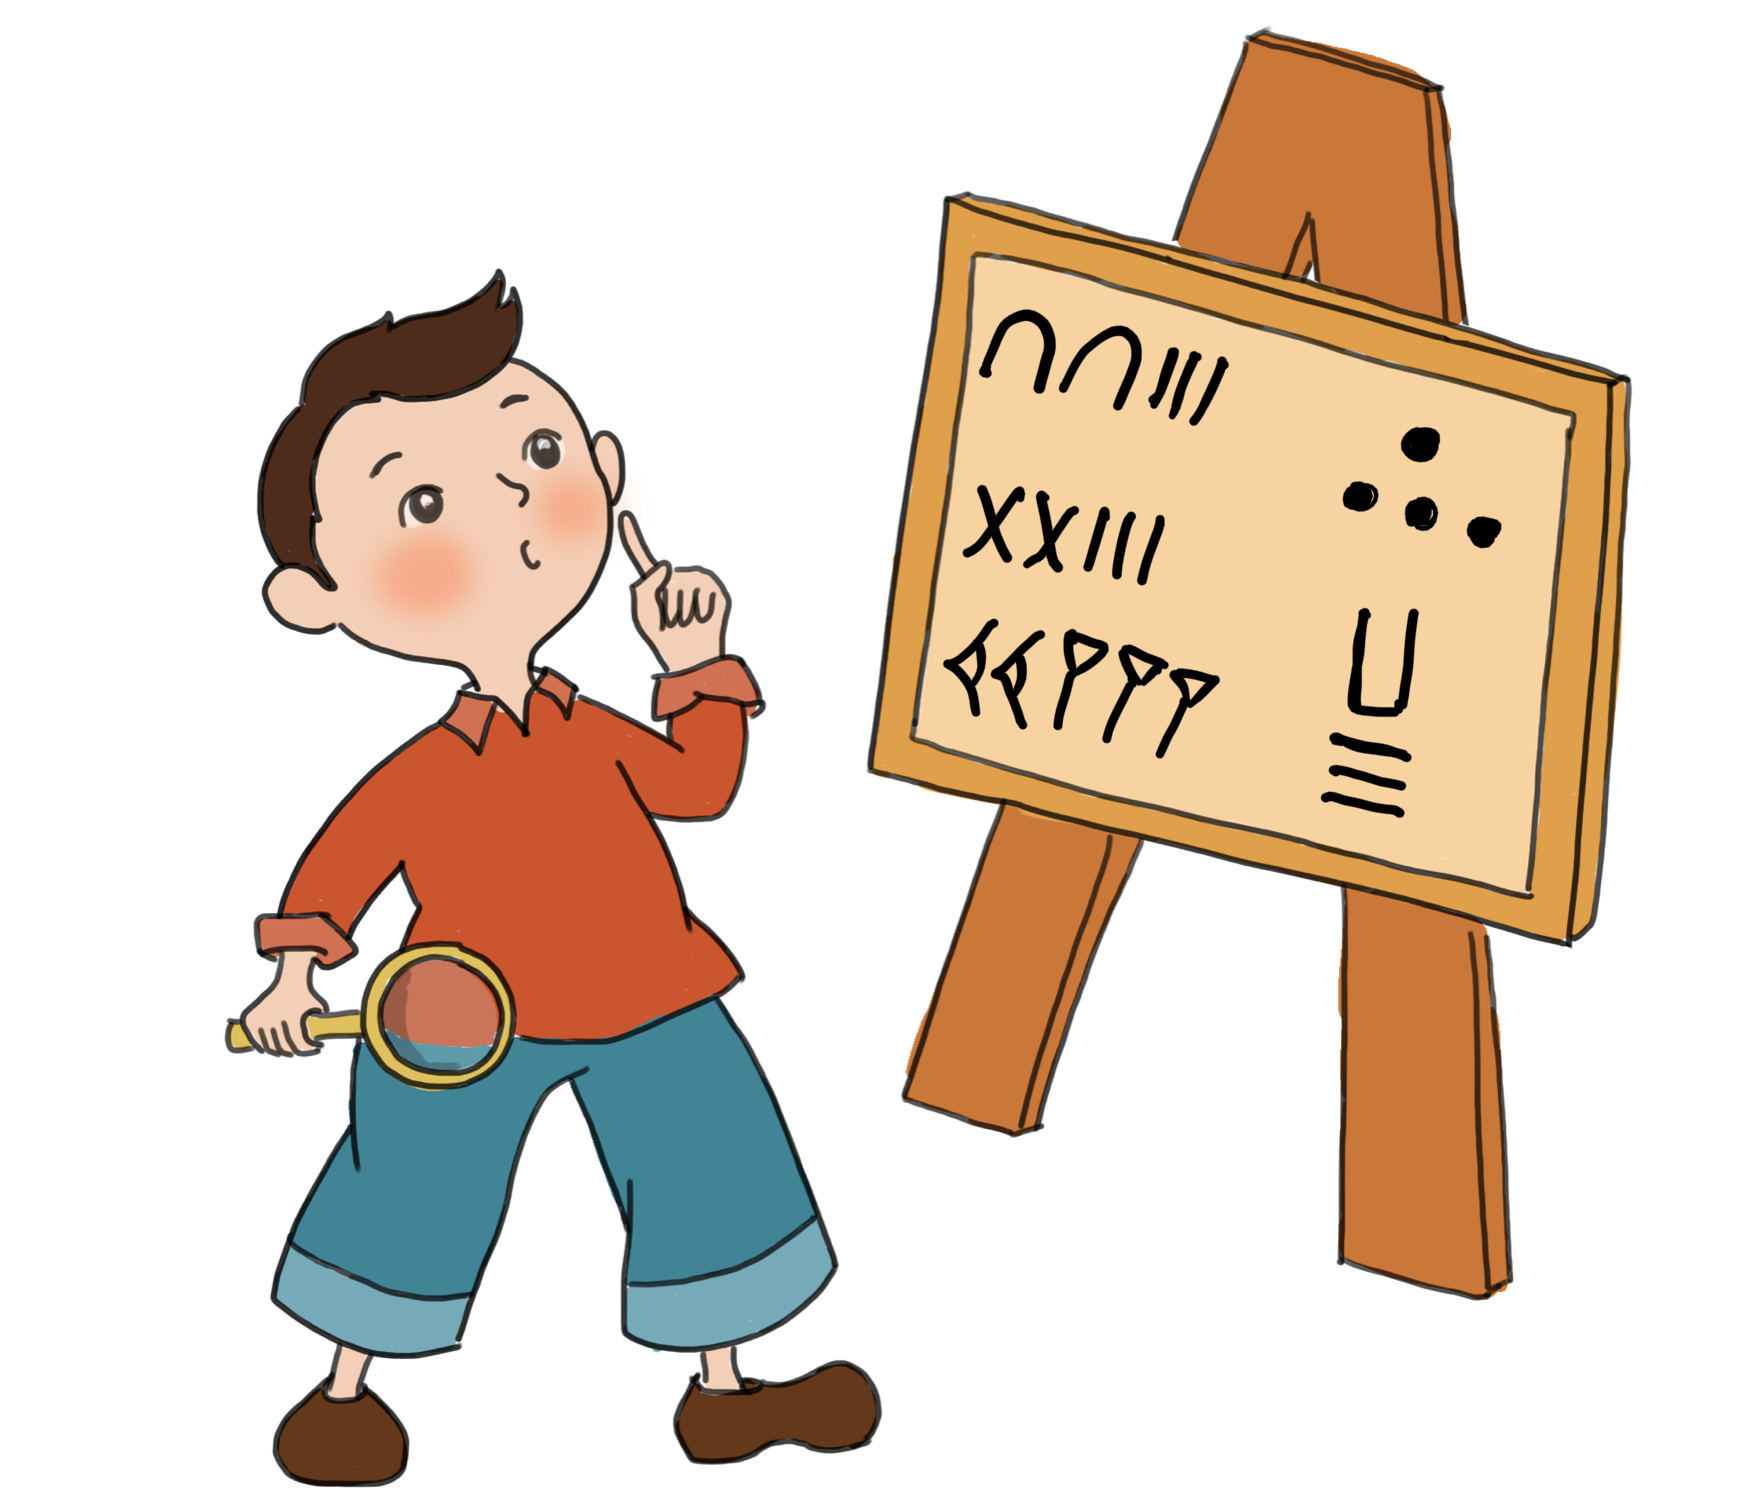
\includegraphics[width=0.8\linewidth]{20.12-pi}
%		\caption{\small\textit{\color{toancuabi}Hình $2$: Số $23$ trong một số hệ ghi số cổ đại.}}
%		\vspace*{-10pt}
%	\end{figure}
%	Đó là những cách ghi số cổ của số $23$. Em có thể đoán xem những ký hiệu nào biểu diễn hàng chục, hàng đơn vị tương ứng với cách chúng ta viết số $23$ ngày nay không?
%	\vskip 0.1cm
%	\textbf{\color{toancuabi}Số Ai Cập cổ}
%	\vskip 0.1cm
%	Ai Cập cổ đại, một trong những cái nôi văn minh của nhân loại, là vùng đất nằm dọc hai bên sông Nile, phía Bắc của châu Phi. Toán học đã xuất hiện ở đây cách đây hơn $5000$ năm. Những thành tựu toán học là một trong những yếu tố quan trọng giúp người Ai Cập cổ xây dựng nên những kim tự tháp mà một số vẫn còn tồn tại đến ngày nay. 
%	\vskip 0.1cm
%	Người Ai Cập cổ sử dụng những ký hiệu bằng hình ảnh để viết các số (được gọi là chữ viết \textit{tượng hình}). Những chữ số của họ như~sau.
%	\end{multicols}
%	\begin{table}[H]
%%		\vspace*{-5pt}
%		\setlength{\tabcolsep}{5.05pt}
%		\renewcommand{\arraystretch}{1.25}
%		\centering
%		\begin{tabular}{|c|c|c|c|c|c|c|}
%			\hline
%			& & & & & & \\[-3ex]
%			
\includegraphics[scale=1]{2a}&
\includegraphics[scale=1]{2b}&
\includegraphics[scale=1]{2c}&
\includegraphics[scale=0.9]{2d}&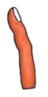
\includegraphics[scale=1]{2e}&
\includegraphics[scale=1]{2f}&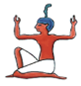
\includegraphics[scale=1]{2g}\\
%			\hline
%			$1$&$10$ &$100$&$1000$&$10000$&$100000$&$1000000$\\
%			\hline
%			{Gạch đứng}&{Móng ngựa}&{Cuộn dây}&{Hoa sen}&{Ngón tay}&{Con ếch}&{Vị thần}\\
%			\hline
%		\end{tabular}
%		\vspace*{-5pt}
%	\end{table}
%	\begin{multicols}{2}
%	Số $4$ được viết là 
\includegraphics[scale=0.85]{3} còn 
\includegraphics{4}  là số $7$. Để viết các số từ $10$ trở lên, người ta dùng thêm ký hiệu 
\includegraphics[scale=0.85]{5} (để biểu diễn số $10$), chẳng hạn số $17$ được viết là 
\includegraphics[scale=0.85]{5}
\includegraphics[scale=0.85]{4} và số $27$ được viết là  
\includegraphics[scale=0.85]{5}
\includegraphics[scale=0.85]{5}
\includegraphics[scale=0.85]{4}. Số lượng các ký hiệu 
\includegraphics[scale=0.85]{5} cho biết có bao nhiêu chục, số các ký hiệu 
\includegraphics[scale=1]{12} cho biết có bao nhiêu đơn vị trong số được biểu diễn. Với những số từ $100$ trở đi họ dùng ký hiệu 
\includegraphics[scale=0.85]{6} (biểu diễn số $100$) và viết các số theo cách tương tự; và cứ như vậy cho những số lớn hơn. Để biết giá trị của số được biểu diễn ta cộng các giá trị ứng với những ký hiệu biểu diễn nó. Chẳng hạn, 
\includegraphics[scale=0.85]{6}
\includegraphics[scale=0.85]{6}
\includegraphics[scale=0.85]{5}\includegraphics[scale=0.85]{5}\includegraphics[scale=0.85]{5}\includegraphics[scale=0.85]{3.1}   $=  100+ 100 + 10 + 10 + 10 + 1 + 1 + 1= 233$.
%	\vskip 0.1cm
%	\begin{figure}[H]
%		\centering
%		\vspace*{-5pt}
%		\captionsetup{labelformat= empty, justification=centering}
%		\includegraphics[width=0.7\linewidth]{20.12-pi.1}
%		\vspace*{-10pt}
%	\end{figure}
%	Ngày nay, ta dùng các hàng khác nhau để biểu diễn số: hàng đơn vị, hàng chục, hàng trăm,... Hàng chục đứng ngay trước hàng đơn vị và lớn gấp $10$ lần hàng đơn vị, hàng trăm đứng ngay trước hàng chục và lớn gấp $10$ lần hàng chục,... Đó là cách ghi số trong hệ ``cơ số $10$" hay ``\textit{thập phân}". Cách ghi số của người Ai Cập cổ cũng vậy nhưng việc viết các số phức tạp hơn so với cách viết ngày nay của chúng ta, nhất là với những số lớn. Chẳng hạn để viết số $5412314$, người Ai Cập cổ cần dùng $20$ ký hiệu!
%	\begin{center}
%		$5412314   =$ \includegraphics[scale=0.85]{7}\includegraphics[scale=0.85]{7}\includegraphics[scale=0.85]{7}\includegraphics[scale=0.85]{7}\includegraphics[scale=0.85]{7}\includegraphics[scale=0.35]{fog.png}\includegraphics[scale=0.35]{fog.png}\includegraphics[scale=0.35]{fog.png}\includegraphics[scale=0.35]{fog.png}\includegraphics[scale=0.85]{9}\includegraphics[scale=0.85]{10}\includegraphics[scale=0.85]{10}\includegraphics[scale=0.85]{6}\includegraphics[scale=0.85]{6}\includegraphics[scale=0.85]{6}\includegraphics[scale=0.85]{5}\includegraphics[scale=0.85]{3}
%	\end{center}
%	\vskip 0.1cm
%	\textbf{\color{toancuabi}Số La Mã}
%	\vskip 0.1cm
%	Các bạn có nhìn thấy các ký hiệu I, II, ..., X trên mặt đồng hồ, trong sách vở, trên bảng khi thầy cô giáo đánh số các mục trong bài giảng? Đó là các số La Mã. La Mã là tên gọi một đế chế cổ đại thuộc châu Âu mà có thời kỳ từng thống trị một vùng đất rộng lớn của châu lục này. Người La Mã sử dụng một số chữ cái từ bảng chữ cái của họ để biểu diễn những chữ số.
%	\vskip 0.1cm
%	Số $4$ được viết là IV, còn số $6$ là VI. Khi một chữ số lớn được viết ngay trước  một chữ số nhỏ hơn hay bằng nó, ta cộng chúng lại với nhau để được con số cần biểu diễn, như trường hợp số $6=$ VI. Ngược lại, ta thực hiện phép trừ, giống như trường hợp số $4=$ IV.
%	\begin{table}[H]
%%		\vspace*{-5pt}
%		\centering
%		\setlength{\tabcolsep}{4.5pt}
%		\renewcommand{\arraystretch}{1.25}
%		\begin{tabular}{|l l|l l|}
%			\hline
%			IV $=4$:&    V$-$I $=$ IV & VI $=6$:&    V$+$I =VI\\
%			&$5-1=4$ & &$5+1=6$\\
%			\hline
%		\end{tabular}
%		\vspace*{-10pt}
%	\end{table}
%	Tương tự, ta có:
%	\begin{table}[H]
%		\vspace*{-10pt}
%		\centering
%		\setlength{\tabcolsep}{3.7pt}
%		\renewcommand{\arraystretch}{1.25}
%		\begin{tabular}{|l l|}
%				\hline
%				XXXII $\!=\! 32$:&    X$+$X$+$X$+$I$+$I $\!=\!$ XXXII\\
%				&$10 +10 +10+1+1=32$\\
%				\hline
%				XL$= 40$:&     L $-$ X = XL\\
%				&$50 - 10 = 40$\\
%				\hline
%		\end{tabular}
%	\end{table}
%	\end{multicols}
%	\begin{figure}[H]
%		\centering
%%		\vspace*{-5pt}
%		\captionsetup{labelformat= empty, justification=centering}
%		\includegraphics[width=1\linewidth]{14a}
%		\caption{\small\textit{\color{toancuabi}Các chữ cái và chữ số La Mã}}
%		\vspace*{-10pt}
%	\end{figure}
%	\begin{multicols}{2}
%	Theo cách người La Mã viết số, khi một chữ số nhỏ đứng trước chữ số số lớn hơn, ta trừ số lớn cho số bé. Trong đó I, V chỉ được trừ từ những giá trị không quá X. Ví dụ, ta có thể viết IX nhưng không thể viết IL; X, L chỉ được trừ bởi những chữ số không vượt quá C; C, D chỉ được trừ cho những chữ số không vượt quá M. Ngoài ra, còn có những quy tắc khác như sau:
%	\vskip 0.1cm
%	-- Luôn viết số bằng cách dùng ít ký hiệu nhất, chẳng hạn ta viết XX để biểu diễn $20$ thay vì VVVV.
%	\vskip 0.1cm
%	-- Không có nhiều hơn $3$ ký tự giống nhau trong một hàng (đơn vị, chục, trăm,...). Ví dụ ta viết XIV thay vì XIIII để biểu diễn $14$.
%	\vskip 0.1cm
%	-- Để biểu diễn số gấp hơn $1000$ lần, người La Mã dùng vạch ngang phía trên các dãy chữ số, ví dụ $\overline{\text{VI}}\text{II}=6\times 1000+2=6002$. Ở đây, VI có thêm vạch ngang trên đầu biểu diễn giá trị $6\times 1000 = 6000$. Những chữ số có vạch ngang trên đầu đứng trước các chữ số còn lại.
%	\vskip 0.1cm
%	-- Không đặt nhiều hơn $1$ số nhỏ đứng trước $1$ số lớn. Ví dụ ta không viết IIX để biểu diễn~$8$.
%	\vskip 0.1cm
%	Để dễ dàng viết số La Mã, ta viết theo từng hàng từ  lớn đến nhỏ (như các số mà ngày nay chúng ta dùng). Ví dụ, để viết số $645$, ta viết $600$ trước (DC), rồi $40$ (XL) và cuối cùng là $5$ (V). Vậy $\text{DCXLV}=645$.
%	Số La Mã là hệ số cổ duy nhất còn được dùng ngày nay nhưng cũng chỉ mang ý nghĩa tượng trưng hay để trang trí.
%	\vskip 0.1cm
%	Trong phần hai của bài viết này chúng ta sẽ cùng tìm hiểu  cách ghi số của người Babylon, Maya và Trung Hoa cổ đại. Mời các em đón đọc ở số báo sau. Còn bây giờ chúng ta cùng làm một số bài tập nhé.
%	\vskip 0.1cm
%	\textbf{\color{toancuabi}Bài tập} $\pmb{1.}$ Viết các số sau theo cách viết số ngày nay
%	\vskip 0.1cm
%	$\bullet$ \includegraphics{5}\includegraphics{5}\includegraphics{4}
%	\vskip 0.1cm $\bullet$ \includegraphics{10}\includegraphics{10}\includegraphics{6}\includegraphics{6}\includegraphics{6}
%	\vskip 0.1cm $\bullet$ \includegraphics{9}\includegraphics{10}\includegraphics{10}\includegraphics{6}\includegraphics{3}
%	\vskip 0.1cm
%	$\bullet$ IX
%	\vskip 0.1cm
%	$\bullet$ CLII
%	\vskip 0.1cm
%	$\bullet$ MCCXXX
%	\vskip 0.1cm
%	\textbf{\color{toancuabi}Bài tập} $\pmb{2.}$ Viết các số sau bằng số Ai Cập cổ và số La Mã
%	\vskip 0.1cm
%	$\bullet$ $8$
%	\vskip 0.1cm
%	$\bullet$ $15$
%	\vskip 0.1cm
%	$\bullet$ $999$

	\textbf{\color{toancuabi}Số Babylon}
	\vskip 0.1cm
	Người Babylon, sống vào khoảng $5000$ năm trước ở vùng đất Lưỡng Hà (một khu vực ở phía Tây của  Châu Á). Họ đã tạo ra những công cụ tính toán thiên văn, hình học đáng kinh ngạc và họ đã phát minh ra bàn tính.
		\begin{figure}[H]
		\centering
		\vspace*{-5pt}
		\captionsetup{labelformat= empty, justification=centering}
		\includegraphics[width=1\linewidth]{17.1}
		\vspace*{-15pt}
	\end{figure}
	Để ghi số, ban đầu người Babylon chỉ sử dụng hai ký hiệu 
	\begin{table}[H]
		\vspace*{-10pt}
		\centering
		\begin{tabular}{|c|c|}
			\hline
			& \\[-2.5ex]
			\includegraphics[scale=0.7]{15}&$1$\\
			\hline
			& \\[-2.5ex]
			\includegraphics[scale=0.65]{16}&$10$\\
			\hline
		\end{tabular}
		\vspace*{-10pt}
	\end{table}
	để viết số từ $1$ tới $60$, chẳng hạn số $7$ là  \includegraphics[scale=0.7]{17}, số $27$ là  \includegraphics[scale=0.7]{16}\includegraphics[scale=0.7]{16}\includegraphics[scale=0.7]{17}. 	 
	\vskip 0.1cm
	Những ký hiệu này được sử dụng tương tự như những chữ số La Mã (bằng cách cộng các ký hiệu xuất hiện trong số được biểu diễn). Số \includegraphics[scale=0.7]{18} được viết bởi $2$ ký hiệu \includegraphics[scale=0.7]{16} để biểu diễn $2$ chục, và $7$ ký hiệu \includegraphics[scale=0.7]{15}  cho $7$ đơn vị. Do vậy \includegraphics[scale=0.7]{18}  $=27$.
	\vskip 0.1cm
	Sau đó, một ký hiệu mới được sử dụng để biểu diễn chữ số $0$ (các bạn có thấy nó là ký tự chỉ chữ số $1$ được viết ngiêng?)
	\includegraphics[scale=0.65]{15.1}
	\vskip 0.1cm
	Để viết những số từ $60$ trở đi, người Babylon xếp các ký hiệu theo các nhóm. Điều này giống như ngày nay các bạn viết $159$ bằng cách viết số $1$ đầu tiên ứng với hàng trăm, số $5$ tiếp theo ở hàng chục và cuối cùng là số $9$ ở hàng đơn vị. Như vậy $159 = 1 \times 100+ 5 \times 10+ 9$.
	\vskip 0.1cm
	\begin{figure}[H]
		\centering
		\vspace*{-5pt}
		\captionsetup{labelformat= empty, justification=centering}
		\includegraphics[width=0.85\linewidth]{20.12-pi.2}
		\vspace*{-15pt}
	\end{figure}
	Để viết số $63$, người Babylon viết ký hiệu  \includegraphics[scale=0.7]{15}  ở hàng $60$ và ba ký hiệu \includegraphics[scale=0.7]{15}  ở hàng đơn vị và để khoảng trống để phân biệt hai nhóm.
	\vskip 0.1cm
	\includegraphics[scale=0.7]{16.1}$=63$. Trong cách viết này, ta thấy có $4$ ký hiệu \includegraphics[scale=0.7]{15}   nhưng ký hiệu đầu tiên được viết tách biệt so với $3$ cái còn lại để biểu diễn $1$ lần $60$ tức $60$, $3$ ký hiệu còn lại biểu diễn số $3$, và như vậy ta có số $60+3 =63$.
	\vskip 0.1cm
	Điều này giống như chúng ta viết chữ số $1$ ở hàng chục và chữ số $1$ ở hàng đơn vị để biểu diễn số $11$: nó có nghĩa là $1$ chục và $1$ đơn vị. Trong  cách ghi số  Babylon cổ, nó có nghĩa là $1$ lần $60$  và $1$.
	\vskip 0.1cm
	Để hiểu rõ hơn, ta hãy viết số chín mươi ba theo hệ ghi số hiện đại. Việc này thật dễ dàng phải không? Tuy nhiên để hiểu cách viết của người Babylon, ta sẽ thực hiện theo cách như sau: do các số của chúng ta ngày nay sử dụng hệ cơ số $10$, ta chia chín mươi ba cho $10$ được thương là $9$, nên ta viết $9$ vào hàng chục
	\begin{figure}[H]
		\centering
		\vspace*{-5pt}
		\captionsetup{labelformat= empty, justification=centering}
		\includegraphics[width=0.65\linewidth]{19}
		\vspace*{-10pt}
	\end{figure}
	Phép chia đó có số dư $3$ nên ta viết $3$ vào hàng đơn vị
	\begin{figure}[H]
		\centering
		\vspace*{-5pt}
		\captionsetup{labelformat= empty, justification=centering}
		\includegraphics[width=0.65\linewidth]{20}
		\vspace*{-10pt}
	\end{figure}
	Vậy là ta viết: $93$.
	\vskip 0.1cm
	Thế còn người Babylon viết số $93$ trong hệ thống số của họ như thế nào?
	\vskip 0.1cm
	\textit{Hệ thống số Babylon sử dụng hệ cơ số $60$}: ta chia $93$ cho $60$ được thương là $1$ nên ta viết $1$ ở hàng $60$
	\begin{figure}[H]
		\centering
		\vspace*{-5pt}
		\captionsetup{labelformat= empty, justification=centering}
		\includegraphics[width=0.65\linewidth]{21}
		\vspace*{-10pt}
	\end{figure}
	Phép chia có số dư là $33$, nên ta sẽ viết $33$ ở hàng đơn vị. Số $33$ được biểu diễn bởi $3$ ký tự mười cộng với $3$. Nên ta đặt $3$ ký tự \includegraphics[scale=0.65]{16} và $3$ ký tự \includegraphics[scale=0.65]{15} vào hàng đơn vị như sau
	\begin{figure}[H]
		\centering
		\vspace*{-5pt}
		\captionsetup{labelformat= empty, justification=centering}
		\includegraphics[width=0.65\linewidth]{22}
		\vspace*{-10pt}
	\end{figure}
	Vậy \includegraphics[scale=0.85]{23}  $= 93$.
	\vskip 0.1cm
	Tiếp theo, chúng ta hãy thử viết số lớn hơn. Chúng ta hãy cùng viết số $3604$ bằng các chữ số Babylon nhé. Số $3604$ lớn hơn $60\times 60=3600$, nên ta cần biểu diễn số này từ hàng thứ ba tính từ hàng đơn vị. Ta chia số $3604$ cho $3600$ được thương là $1$ nên ta viết ký hiệu \includegraphics[scale=0.7]{15}  vào hàng $60\times60$
	\begin{figure}[H]
		\centering
		\vspace*{-5pt}
		\captionsetup{labelformat= empty, justification=centering}
		\includegraphics[width=0.65\linewidth]{25}
		%	\caption{\textit{\color{toancuabi}Hình $1$.}}
		\vspace*{-10pt}
	\end{figure}
	Số dư của phép chia là $4$ nhỏ hơn $60$ nên ta viết ký hiệu \includegraphics[scale=0.6]{15.1} vào hàng $60$, và $4$ ký hiệu \includegraphics[scale=0.7]{15} vào hàng đơn vị. 
	\begin{figure}[H]
		\centering
		\vspace*{-5pt}
		\captionsetup{labelformat= empty, justification=centering}
		\includegraphics[width=0.65\linewidth]{26}
		%	\caption{\textit{\color{toancuabi}Hình $1$.}}
		\vspace*{-10pt}
	\end{figure}
	Vậy, số $3604$ được người Babylon viết như sau:
	\begin{figure}[H]
		\centering
%		\vspace*{-5pt}
		\captionsetup{labelformat= empty, justification=centering}
		\includegraphics[width=0.75\linewidth]{27}
		%	\caption{\textit{\color{toancuabi}Hình $1$.}}
		\vspace*{-10pt}
	\end{figure}
	Cách ghi Số của người Ai Cập cổ, La Mã hay chúng ta ngày nay dùng cơ số $10$ còn cách ghi số của người Babylon sử dụng cơ số $60$. Do số $60$ chia hết cho nhiều số: $1,2,3,4,5,6, 10, 12, 15, 20,30$ và $60$, nên việc chia các đại lượng được thực hiện dễ dàng hơn, ít phải dùng đến các phân số. Việc sử dụng đơn vị thời gian: $1$ phút $= 60$ giây, $1$ giờ $= 60$ phút ngày nay là một ảnh hưởng của người Babylon đấy.
	\vskip 0.1cm
	\textbf{\color{toancuabi}Số Maya}
	\vskip 0.1cm
	\begin{figure}[H]
		\centering
		\vspace*{-10pt}
		\captionsetup{labelformat= empty, justification=centering}
		\includegraphics[width=1\linewidth]{28}
		\caption{\textit{\color{toancuabi}Kim tự tháp Tikal của người Maya}}
		\vspace*{-15pt}
	\end{figure}
	Người Maya  được cho là đã xuất hiện từ rất xa xưa. Họ đã xây dựng hệ thống lịch chính xác và toán học của họ là đại diện tiêu biểu cho toán học của dân cư ở châu Mỹ thời cổ đại.
	\vskip 0.1cm
	Nói về cách ghi số,  người Maya  cổ dùng hệ cơ số $20$, gồm $3$ ký hiệu:  \includegraphics[scale=0.7]{29},  \includegraphics[scale=0.7]{30}, \includegraphics[scale=0.7]{31}  ứng với $0,1, 5$ và biểu diễn số theo chiều dọc. Chữ số ở hàng cao hơn được viết phía trên, chữ số ở hàng thấp hơn được viết phía dưới. Điều này tương tự chúng ta viết số ngày nay: ta đặt số ở hàng cao hơn bên trái còn số ở hàng thấp hơn bên phải. 
	\begin{table}[H]
		\vspace*{-5pt}
		\centering
		\setlength{\tabcolsep}{4.5pt}
		\renewcommand{\arraystretch}{1.25}
		\begin{tabular}{|l|l|}
			\hline
			$10^3 = 10\!\times\! 10 \!\times\! 10 =1000$& hàng nghìn\\
			\hline
			$10^2 = 10\!\times\! 10 =100$& hàng trăm\\
			\hline
			$10^1 = 10$& hàng chục\\
			\hline
			$10^0 = 1$& hàng đơn vị\\
			\hline
		\end{tabular}
%		\vspace*{-5pt}
	\end{table}
	Do sử dụng hệ cơ số $20$,  số Maya được biểu diễn trong phần bên phải của bảng trong Hình $3$ chính là số  $1\times 8000+ 0\times 400+ 10\times20+ 7\times1= 8207$. Bởi vì, ta  thấy  \includegraphics[scale=0.3]{33},  \includegraphics[scale=0.3]{34},  \includegraphics[scale=0.3]{35}, \includegraphics[scale=0.3]{36}  ứng với $1, 0, 10, 7$  lần lượt ở các hàng $8000$, $400$, $20$ và đơn vị. Chú ý rằng, trong một hàng, số có giá trị cao hơn lại được viết phía dưới số có giá trị lớn hơn chẳng hạn  \includegraphics[scale=0.3]{36}:  hai ký tự \includegraphics[scale=0.7]{37} (số $1$) được viết bên trên ký tự \includegraphics[scale=0.7]{38} (số $5$). Ký hiệu \includegraphics[scale=0.3]{34} để biểu diễn $0$ ở một hàng giống như ta viết $101$ và giúp ta phân biệt số $101$ với số $11$. Điều này cũng tương tự như cách ghi số Babylon. 
	\begin{table}[H]
		\vspace*{-5pt}
		\centering
		\captionsetup{labelformat= empty, justification=centering}
		\setlength{\tabcolsep}{21pt}
		\renewcommand{\arraystretch}{1.25}
		\begin{tabular}{|l|c|}
			\hline
			$20\times 20\times 20 =8000$  & \includegraphics[scale=0.3]{33} \\
			\hline
			$20\times 20 =400$     & \includegraphics[scale=0.3]{34} \\
			\hline
			$20$ & \includegraphics[scale=0.3]{35}\\
			\hline
			$1$& \includegraphics[scale=0.3]{36.png}\\
			\hline
		\end{tabular}
		\caption{\small\textit{\color{toancuabi}Hình $3$.}}
		\vspace*{-10pt}
	\end{table}
	Người ta cho rằng hệ cơ số $10$ được dùng phổ biến vì con người có $10$ ngón tay, còn người Maya vốn không đi giày nên họ đếm bằng cả các ngón chân nữa. Họ dùng hệ cơ số $20$ là vì thế!
	\begin{figure}[H]
		\centering
		\vspace*{-5pt}
		\captionsetup{labelformat= empty, justification=centering}
		\includegraphics[width=1\linewidth]{20.12-pi.4-2}
		\vspace*{-12pt}
	\end{figure}
	\vskip 0.1cm
	\textbf{\color{toancuabi}Số Trung Hoa cổ}
	\vskip 0.1cm
	Trung Hoa cổ đại cũng là một trong những nền văn minh cổ lớn của thế giới. Khoảng $3500$ năm trước, người Trung Hoa khắc lên những mảnh mai rùa những ký hiệu khác nhau thể hiện số và chữ. Một số trong đó như~sau:
	\begin{figure}[H]
		\centering
%		\vspace*{-5pt}
		\captionsetup{labelformat= empty, justification=centering}
		\includegraphics[height=0.45\linewidth]{40}\quad
		\includegraphics[height=0.45\linewidth]{41}
		\caption{\textit{\color{toancuabi}Một số ký hiệu viết trên một mảnh mai rùa.}}
		\vspace*{-10pt}
	\end{figure}
	Cách ghi số Trung Hoa cổ tương tự như cách ghi số La Mã: Các chữ số giá trị lớn được đặt bên trái các chữ số có  giá trị nhỏ hơn, số được biểu diễn có giá trị bằng tổng các chữ số trong biểu diễn của nó. Ví dụ \includegraphics[scale=0.7]{42} biểu diễn số $10000 + 500 + 30 + 5 =10535$. Những biểu tượng khắc trên những mảnh mai rùa phát triển theo thời gian và hình thành nên chữ viết của người Trung Hoa ngày nay. 
	\vskip 0.1cm
	Các bạn có thấy rằng cách biểu diễn số của người Ai Cập, La Mã và Trung Hoa cổ có điểm tương đồng? Người ta nói đó là những hệ thống số ``\textit{đơn phân}". Mỗi ký hiệu thể hiện một giá trị không thay đổi cho dù nó đứng ở vị trí nào. Mỗi số viết ra biểu diễn một đại lượng được xác định bằng cách  cộng (hay trừ như ở số La Mã) những giá trị tương ứng với các ký hiệu được sử dụng trong đó. Số mà chúng ta dùng ngày nay là một hệ thống số ``\textit{sắp theo hàng}" vì các ký hiệu có giá trị phụ thuộc vào hàng mà nó được xếp vào. Ở hàng chục, số $1$ có nghĩa là một chục, nhưng số $1$ ở hàng đơn vị có nghĩa là $1$ đơn vị. Trong khi đó, số của người Babylon và Maya là một dạng hỗn hợp vừa được ``\textit{sắp theo hàng}" vừa cần cộng những ký hiệu trong mỗi hàng để biết giá trị của số được biểu diễn.
	\begin{figure}[H]
		\centering
		\vspace*{-5pt}
		\captionsetup{labelformat= empty, justification=centering}
		\includegraphics[width=0.85\linewidth]{20.12-pi.3}
		\vspace*{-10pt}
	\end{figure}
	Vậy là qua bài viết này chúng ta đã biết những cách ghi số  từ thời xa xưa con người ở những nơi khác nhau trên Trái Đất. Những đại lượng phức tạp hơn như phân số chẳng hạn cũng đã được người cổ đại viết ra và sử dụng. Chúng ta sẽ tìm hiểu thêm về những thành tựu toán học của loài người ở những thời kỳ trước đây trong những số báo sắp tới nhé. 
	\vskip 0.1cm
	\textbf{\color{toancuabi}Tài liệu, nguồn tham khảo}
	\vskip 0.1cm
	[$1$] R. L. Cooke, History of math, Wiley, $2013$.
	\vskip 0.1cm
	[$2$] \url{https://www.britannica.com/}
	\vskip 0.1cm
	[$3$] \url{https://www.penn.museum/}
	\vskip 0.1cm
	[$4$] \url{https://www.cemc.uwaterloo.ca}
\end{multicols}
%\newpage
%\graphicspath{{../toancuabi/pic/}}
%\begingroup
%\AddToShipoutPicture*{\put(112,680){\includegraphics[scale=1]{../tieude.pdf}}} 
%\centering
%\endgroup
%\vspace*{25pt}
%
%\begin{multicols}{2}
%	Một lần nọ, thám tử Xuân Phong lên đường để truy tìm một kẻ tội phạm có biệt hiệu là Bắp Cải đang lẩn trốn trong một khu lán trại hẻo lánh có tên là Vườn Ngô. Xuân Phong vừa đi vừa hỏi đường vì bản đồ không chỉ rõ khu Vườn Ngô ở đâu, chắc hẳn đó là một địa điểm mới trong vùng. Thám tử đang lơ ngơ tìm đường thì bỗng nhiên một bác nông dân vui tính, tay cầm cuốc, mồ hôi nhễ nhại, xuất hiện trước mặt. Bác hồ hởi vừa nói vừa đưa tay ra hiệu: ``Tôi biết đường đến khu Vườn Ngô chứ, tôi đã từng đến đó rồi. Lần đó, tôi đi mất  tận $4$ ngày và $4$ đêm. Ngày và đêm đầu tiên tôi đi trên đường cái thẳng về phía bắc, và đi được một phần ba quãng đường. Sau đó tôi quay về phía tây và gắng sức đi xuyên qua rừng mất một ngày một đêm nữa, và đi được quãng đường chỉ bằng nửa của ngày đêm đầu tiên. Ngày và đêm thứ ba tôi lại phải đi xuyên qua rừng tiếp, và đi về phía nam và cuối cùng lại đi ra đường cái dẫn về phía đông. Tôi đi rảo bước theo con đường đó cả ngày cả đêm thứ tư, đi hết $30$ km và thế là đặt chân đến được khu Vườn Ngô, nơi mà thám tử đang tìm. Đấy, thám tử cứ đi theo con đường sáng suốt như tôi đã đi là thế nào sang tới ngày thứ $5$ sẽ tới được Vườn Ngô".
%	\vskip 0.1cm
%	Xuân Phong suy nghĩ một chút rồi xua tay trả lời ``Cảm ơn bác nhé. Nếu mọi thứ cứ đúng như bác nói thì ngay ngày mai tôi đã có thể đặt chân tới Vườn Ngô và bắt được tên Bắp~Cải."
%	\begin{figure}[H]
%		\centering
%		\vspace*{-5pt}
%		\captionsetup{labelformat= empty, justification=centering}
%		\includegraphics[width=1\linewidth]{xp}
%		\vspace*{-15pt}
%	\end{figure}
%	Xuân Phong có lập luận đúng không nhỉ? Theo em, bác nông dân đã đi bao nhiêu km để tới Vườn Ngô, còn Xuân Phong thì nghĩ sẽ cần phải đi hết bao nhiêu km?
%\end{multicols}
%\vspace*{-10pt}
%\rule{1\linewidth}{0.1pt}
%\begingroup
%\AddToShipoutPicture*{\put(112,248){\includegraphics[scale=1]{../tieude11.pdf}}} 
%\centering
%\endgroup
%\vspace*{40pt}
%
%\begin{multicols}{2}
%	$\pmb{1.}$ Một lần nọ, sau cơn mưa, bác Tuấn đi vào rừng để hái nấm. Bác khệ nệ bê được cả một sọt nấm nặng trĩu về. Nhưng thật buồn cho bác là về đến nhà, bác mới biết là trong số nấm tươi mới hái được thì có tới tận $90\%$ thành phần là nước, nên hoá ra bác mất công mang nước về suốt cả một quãng đường dài. Sau khi nấm được hong khô đi chút, khối lượng của đống nấm bị giảm đi $15$ kg, và bây giờ nước chỉ chiếm $60\%$ khối lượng. Hỏi lúc đầu bác Tuấn đã mang được bao nhiêu ki--lô--gam nấm từ rừng về nhà?
%	
%	\columnbreak
%	\begin{figure}[H]
%		\centering
%%		\vspace*{5pt}
%		\captionsetup{labelformat= empty, justification=centering}
%		\includegraphics[width=0.65\linewidth]{bai1}
%	\end{figure}
%	\end{multicols}
%	\begin{multicols}{2}
%	$\pmb{2.}$ Ông Ninh cùng với con trai mình và ông Phúc cùng với con trai mình đi ra hồ câu cá. Ông Ninh bắt được số con cá bằng với số con cá mà con trai ông  bắt được. Còn ông Phúc lại bắt được số con cá nhiều gấp ba lần số con cá mà con trai ông bắt được. Họ bắt được tổng cộng  $35$ con. Con trai của ông Ninh đi câu cá cùng ông tên là Giao. Hỏi con ông Phúc tên là gì và mỗi người hôm đó bắt được bao nhiêu con cá?
%	\begin{figure}[H]
%		\centering
%		\vspace*{-5pt}
%		\captionsetup{labelformat= empty, justification=centering}
%		\includegraphics[width=1\linewidth]{bai2}
%		\vspace*{-15pt}
%	\end{figure}
%	$\pmb{3.}$ Chiếc đồng hồ treo tường nhà bạn Lâm chỉ  $9$ giờ $20$ phút. Hỏi lúc đó góc tạo bởi kim giờ và kim phút bằng bao nhiêu độ (góc tương ứng với một vòng tròn là $360$ độ)?
%	\begin{figure}[H]
%		\centering
%		\vspace*{-5pt}
%		\captionsetup{labelformat= empty, justification=centering}
%		\includegraphics[width=1\linewidth]{bai3}
%		\vspace*{-15pt}
%	\end{figure}
%	$\pmb{4.}$ Tích của một tỷ số tự nhiên bằng đúng $1$ tỷ. Hỏi giá trị lớn nhất của tổng của chúng bằng bao nhiêu?
%	\begin{figure}[H]
%		\centering
%		\vspace*{5pt}
%		\captionsetup{labelformat= empty, justification=centering}
%		\includegraphics[width=1\linewidth]{bai5}
%		\vspace*{-15pt}
%	\end{figure}
%	$\pmb{5.}$ Làm thế nào để xác định tâm của một hình tròn nếu chỉ có một cái bút chì và một cái thước kẻ thông thường có hai cạnh song song (chiều rộng của thước kẻ nhỏ hơn đường kính của hình tròn).
%	\begin{figure}[H]
%		\centering
%		\vspace*{-5pt}
%		\captionsetup{labelformat= empty, justification=centering}
%		\includegraphics[width=1\linewidth]{bai4}
%		\vspace*{-15pt}
%	\end{figure}
%	$\pmb{6.}$ Tất cả các điểm của một đường tròn được tô bằng hai màu: trắng hoặc đỏ. Em hãy chứng tỏ rằng luôn có một tam giác cân có các đỉnh nằm trên đường tròn đã cho sao cho các đỉnh của nó đều được tô bởi cùng một màu.
%	\begin{figure}[H]
%		\centering
%		\vspace*{-5pt}
%		\captionsetup{labelformat= empty, justification=centering}
%		\includegraphics[width=1\linewidth]{bai6}
%		\vspace*{-5pt}
%	\end{figure}
%\end{multicols}
%\newpage
%\begingroup
%\AddToShipoutPicture*{\put(112,640){\includegraphics[scale=1]{../tieude2.pdf}}} 
%\centering
%\endgroup
%\graphicspath{{../toancuabi/pic/}}
%\vspace*{70pt}
%
%\begin{multicols}{2}
%	$\pmb{1.}$	Trong một giải thi đấu bóng chuyền, mỗi đội sẽ lần lượt thi đấu với các đội còn lại hai lần. Cuối cùng người ta thấy rằng $80\%$ các đội có ít nhất một trận thắng. Hỏi có tất cả bao nhiêu đội đã tham gia trong giải đấu đó biết rằng các trận đấu bóng chuyền không có tỷ số hoà?
%	\begin{figure}[H]
%		\vspace*{-5pt}
%		\centering
%		\captionsetup{labelformat= empty, justification=centering}
%		\includegraphics[width= 1\linewidth]{b5}
%		\vspace*{-15pt}
%	\end{figure}
%	\textit{Lời giải.} 	Do trong môn bóng chuyền không có trận hoà, nên đội nào không thắng ít nhất một trận có nghĩa là đội đó thua tất cả các đội còn lại. Nhưng chỉ có thể có duy nhất một đội là như vậy, vì không thể có hai đội $A$, $B$ mà $A$ thua $B$ đồng thời $B$ thua $A$ trong cùng trận đấu. Vì thế $20\%$ số các đội bao gồm đúng duy nhất $1$ đội, có nghĩa là  chỉ có đúng $5$ đội tham gia giải đấu đó.
%	\vskip 0.1cm
%	$\pmb{2.}$	Một buổi cắm trại có $9$ học sinh nam và $10$ học sinh nữ tham gia. Trước đó, mỗi học sinh nam đều đã quen với cùng một số lượng các học sinh nữ tham gia buổi cắm trại đó, còn tất cả các học sinh nữ đều quen số lượng học sinh nam hoàn toàn khác nhau (không có hai em nữ nào có số lượng bạn nam quen biết giống nhau). Hỏi điều này có thể xảy ra hay không?
%	\begin{figure}[H]
%		\vspace*{5pt}
%		\centering
%		\captionsetup{labelformat= empty, justification=centering}
%		\includegraphics[width= 1\linewidth]{b4}
%		\vspace*{-15pt}
%	\end{figure}
%	\textit{Lời giải.} 	Giả sử mỗi học sinh nam quen $k$ học sinh nữ, thì khi đó có tất cả $9k$ mối quen biết. Do các bạn nữ có số bạn nam quen biết là hoàn toàn khác nhau, nên điều này chỉ có thể xảy ra nếu một bạn quen với tất cả $9$ bạn nam, một bạn quen với $8$ bạn nam, vv... và cuối cùng có một bạn không quen bạn nam nào. Vì thế số mối quen biết sẽ là $9+8+7+\cdots+1+0=45$. Do đó $9k=45$, tức là $k=5$. Có thể dễ dàng chỉ ra một sơ đồ quen biết như sau. Ở bảng dưới đây, dấu ``$+$" biểu diễn học sinh nam và học sinh nữ quen biết nhau với số thứ tự được chỉ ra theo chiều ngang và chiều dọc tương ứng.
%	\begin{figure}[H]
%		\centering
%		\vspace*{-5pt}
%		\captionsetup{labelformat= empty, justification=centering}
%		\begin{tikzpicture}[scale=0.5]
%			\draw (6,10) node[above] {Bạn nữ};
%			\draw (-1.5,6) node[left,rotate=90] {Bạn nam};
%			\foreach \x in {1,...,10}{
%					\draw(\x +0.5,9.5) node{$\x$};
%			}
%			\foreach \y in {1,...,9}{
%				\draw(-0.5,9.5-\y) node{$\y$};
%				\draw(10.5,9.5-\y) node{$+$};
%			}
%			\foreach \y in {2,...,9}{
%				\draw(9.5,9.5-\y) node{$+$};
%			}
%			\foreach \y in {3,...,9}{
%				\draw(8.5,9.5-\y) node{$+$};
%			}
%			\foreach \y in {4,...,9}{
%				\draw(7.5,9.5-\y) node{$+$};
%			}
%			\foreach \y in {5,...,9}{
%				\draw(6.5,9.5-\y) node{$+$};
%			}
%			\foreach \y in {1,...,4}{
%				\draw(5.5,9.5-\y) node{$+$};
%			}
%			\foreach \y in {1,...,3}{
%				\draw(4.5,9.5-\y) node{$+$};
%			}
%			\draw(3.5,8.5) node{$+$};
%			\draw(3.5,7.5) node{$+$};
%			\draw(2.5,8.5) node{$+$};
%			\draw[cackithi] (0,0) grid (11,9);
%		\end{tikzpicture}
%	\end{figure}
%	$\pmb{3.}$	Trên bảng có ghi ít nhất hai số nguyên đôi một khác nhau. Hơn nữa tổng của hai số bất kỳ trong chúng cũng được ghi trên đó. Hỏi có bao nhiêu số được viết ra trên bảng?
%	\vskip 0.1cm
%	\textit{Lời giải.} 	Ta sẽ chỉ ra rằng trên bảng không thể có nhiều hơn $1$ số nguyên dương. Thật vậy, giả sử $M$ là số nguyên dương lớn nhất trong các số được viết trên bảng, hơn nữa giả sử có thêm một số nguyên dương $m$ nữa nhỏ hơn, tức là $0<m<M$. Khi đó trên bảng phải có cả số $m+M$, lớn hơn $M$, và điều này là không thể. Tương tự cũng chỉ ra được rằng trên bảng có không quá $1$ số nguyên âm. Như vậy trên bảng hoặc có $2$, hoặc có $3$ số được viết ra. Ví dụ như $2$ số $\{0, 4\}$, hoặc $3$ số $\{-4,0,4\}$.
%	\vskip 0.1cm
%	$\pmb{4.}$ Một số các bạn học sinh lớp $7$ đứng xếp thành hàng ngang. Trước mặt mỗi bạn lại có một học sinh lớp $6$ thấp hơn mình. Em hãy chứng tỏ rằng nếu hai hàng ngang của các học sinh hai lớp được xếp lại tăng dần theo chiều cao ở mỗi hàng, thì ở hai hàng mới, mỗi học sinh lớp $7$ lại vẫn có trước mặt một học sinh lớp $6$ thấp hơn mình.
%	\begin{figure}[H]
%		\vspace*{-5pt}
%		\centering
%		\captionsetup{labelformat= empty, justification=centering}
%		\includegraphics[width= 1\linewidth]{b1}
%		\vspace*{-15pt}
%	\end{figure}
%	\textit{Lời giải.} Ta sẽ thực hiện cách đổi chỗ từng cặp học sinh một  như sau: bắt đầu từ bạn lớp $6$ cao nhất, đổi chỗ bạn cao nhất cho bạn hiện tại đang đứng ở vị trí thứ nhất; tiếp theo bạn cao thứ nhì đổi chỗ cho bạn đang đứng ở vị trí thứ $2$.  Cứ mỗi lần đổi chỗ hai bạn lớp $6$ để sắp xếp theo thứ tự giảm dần, các bạn học sinh lớp $7$ đứng đối diện hai bạn đó cũng được đổi giống như vậy. Sau khi các bạn lớp $6$ đã được xếp theo thứ tự ``đúng", có nghĩa là giảm dần theo chiều cao thì ở hàng của các bạn lớp $7$, vị trí còn khá lộn xộn, chưa được xếp ``đúng chỗ". Tuy nhiên vì mỗi lần đổi chỗ $2$ bạn lớp $6$ ta lại đổi $2$ bạn lớp $7$ đứng đối diện, nên các cặp đứng đối diện vẫn giữ nguyên chưa thay đổi sau khi sắp xếp các bạn lớp $6$ theo thứ tự giảm dần.
%	\vskip 0.1cm
%	Bây giờ ta giữ nguyên hàng của các bạn lớp $6$, và tiến hành xếp các bạn lớp $7$ theo thứ tự chiều cao giảm dần. Đầu tiên bạn cao nhất sẽ được đổi chỗ cho bạn đứng ở vị trí thứ nhất, rồi tiếp tới bạn cao nhì ... Các em có thể thấy ngay cứ sau mỗi lần đổi chỗ như thế ở hàng của lớp  thì trước mặt mỗi bạn lớp $7$ vẫn có một bạn lớp $6$ có chiều cao thấp hơn. Vì vậy cuối cùng sau khi xếp ngay ngắn hàng lớp $7$ giảm dần theo chiều cao thì điều kiện đặt ra của bài toán vẫn được đảm bảo.
%	\vskip 0.1cm
%	$\pmb{5.}$	Trên một bàn cờ vua người ta đặt một số quân cờ mà ở  mỗi một hàng ngang và mỗi hàng dọc của bàn cờ đều có một số lẻ các quân cờ. Em hãy chứng tỏ rằng có một số chẵn các quân cờ đứng ở các ô màu đen của bàn cờ đó.
%	\begin{figure}[H]
%		\vspace*{-5pt}
%		\centering
%		\captionsetup{labelformat= empty, justification=centering}
%		\includegraphics[width= 1\linewidth]{b2}
%		\vspace*{-15pt}
%	\end{figure}
%	\textit{Lời giải.} Đánh số bàn cờ các cột dọc, hàng ngang từ $1$ tới $8$ như trong hình minh hoạ sau. Tại các cột đánh số lẻ (các cột $1$, $3$, $5$, $7$), ta đặt chữ $A$ vào các ô đen, tại các cột còn lại ($2$, $4$, $6$, $8$) ta lại đặt chữ $B$ vào mỗi ô đen. Tại các hàng ngang đánh số chẵn (hàng $2$, $4$, $6$, $8$), ta đặt chữ $C$ vào mỗi ô trắng.
%	\vskip 0.1cm 
%	Số các quân cờ đặt tại các ô $A$ được ký hiệu là $n$, số quân cờ đặt tại các ô $B$ là $m$, và tại các ô $C$ là $k$. 
%	\vskip 0.1cm
%	Các chữ $A,C$ phủ kín các hàng $2,4,6,8$. Mà tại mỗi hàng đó:  tổng số quân cờ là số lẻ theo giả thiết.
%	\begin{figure}[H]
%		\centering
%		\vspace*{-5pt}
%		\captionsetup{labelformat= empty, justification=centering}
%		\begin{tikzpicture}[scale=0.55]
%			\draw[cackithi] (1,1) grid (9,9);
%			\foreach \x in {1,...,8}{
%				\draw (0.5,9.5-\x) node{$\x$};
%				\draw (\x+0.5,9.5) node{$\x$};
%			}
%			\foreach \x in {1,3,...,7}{
%				\foreach \y in {1,3,...,7}{
%					\draw[cackithi,fill=cackithi!50] (\x,\y) rectangle (\x+1, \y+1);
%					\draw (\x+0.5,\y+0.5) node{$A$};
%				}
%			}
%			\foreach \x in {2,4,...,8}{
%				\foreach \y in {2,4,...,8}{
%					\draw[cackithi,fill=cackithi!50] (\x,\y) rectangle (\x+1, \y+1);
%					\draw (\x+0.5,\y+0.5) node{$B$};
%				}
%			}
%			\foreach \x in {2,4,...,8}{
%				\foreach \y in {1,3,...,7}{
%					\draw (\x+0.5,\y+0.5) node{$C$};
%				}
%			}
%		\end{tikzpicture}
%	\end{figure}
%	Vậy $n+k$ là tổng số quân cờ tại bốn hàng đánh số chẵn và là tổng của $4$ số lẻ, nên nó là một số chẵn.
%	\vskip 0.1cm
%	Lập luận tương tự tại các cột $2,4,6,8,$  ta có $m+k$ là số chẵn.
%	Vì thế số các quân cờ đặt tại các ô đen là $m+n$ và là một số chẵn.
%	\vskip 0.1cm
%	$\pmb{6.}$	Bốn chú lùn cùng đi chẻ củi để chuẩn bị cho một mùa đông có nàng Bạch Tuyết tới ở cùng, họ chẻ mất  $3$ tiếng đồng hồ. Nếu như chú lùn thứ nhất làm nhanh gấp đôi, còn chú thứ hai làm chậm một nửa, thì $4$ chú cũng sẽ hoàn thành trong từng đó thời gian. Còn nếu như, ngược lại, chú thứ nhất làm chậm một nửa, còn chú thứ hai làm nhanh gấp đôi, thì họ sẽ xoay sở  đống củi chỉ trong $2$ tiếng.
%	\vskip 0.1cm
%	Hỏi $3$ chú lùn đầu tiên sẽ chẻ hết đống củi trong bao nhiêu lâu mà không cần sự trợ giúp của chú thứ tư?
%	\vskip 0.1cm
%	\textit{Lời giải.} 	Ký hiệu $a$ là số phần của đống củi mà chú lùn thứ nhất chẻ được trong $1$ tiếng, tương tự $b, c,d$ là số phần đống củi mà các chú lùn còn lại chẻ được trong một tiếng. Khi đó ta có
%	\begin{align*}
%		a+b+c+d      &= \frac{1}{3},\\
%		2a+\frac{b}{2}+c+d    &= \frac{1}{3},\\
%		\frac{a}{2}+2b+c+d    &= \frac{1}{2}.
%	\end{align*}
%	Từ hai hệ thức đầu ta thấy $2a=b$.
%	\vskip 0.1cm
%	Trừ hệ thức thứ $3$ cho hệ thức thứ nhất ta có $b-\dfrac{a}{2}=\dfrac{1}{6}$.
%	\begin{figure}[H]
%		\vspace*{-5pt}
%		\centering
%		\captionsetup{labelformat= empty, justification=centering}
%		\includegraphics[width= 1\linewidth]{b6}
%		\vspace*{-15pt}
%	\end{figure}
%	Suy ra $a= \dfrac{1}{9}$, và $b=\dfrac{2}{9}$. Thay vào một trong hai hệ thức đầu ta tìm ra $c+d=0$. Có nghĩa là $2$ chú lùn thứ $3$ và thứ $4$ không động chân động tay làm gì hết ($c=d=0$, do $c,d$ là các số không âm).
%	Vì thế có vắng chú nào trong hai chú này thì thời gian chẻ củi cũng không bị ảnh hưởng. Vậy ba chú lùn đầu vẫn sẽ  chẻ xong đống củi trong thời gian $3$ tiếng như~vậy.
%\end{multicols}
%\newpage
%\begingroup
%\thispagestyle{toancuabinone}
%\AddToShipoutPicture*{\put(60,733){\includegraphics[width=17.2cm]{../mathc.pdf}}}
%%\AddToShipoutPicture*{\put(-2,733){\includegraphics[width=17.2cm]{../mathl.pdf}}} 
%\AddToShipoutPicture*{\put(162,677){\includegraphics[scale=1]{../tieude3.pdf}}} 
%\centering
%\endgroup
%\graphicspath{{../toancuabi/pic/}}
%\vspace*{25pt}
%
%\begin{multicols}{2}
%	\setlength{\abovedisplayskip}{4pt}
%	\setlength{\belowdisplayskip}{4pt}
%	A Magic Triangle is an arrangement of the integers from $1$ to $n$ on the sides of a triangle such that each side has the same number of integers, called the order of the triangle, and that the sum of integers on each side is a constant, called the magic sum of the triangle. A Magic Triangle is also called a Perimeter Magic Triangle.
%	\vskip 0.1cm
%	Now let’s try to build some Magic Triangles!
%	\vskip 0.1cm
%	\PIbox{
%	\textbf{\color{toancuabi}Problem} $\pmb{1}$ ({\color{toancuabi}Magic Triangle of order $3$ and magic sum $9$})\textbf{\color{toancuabi}.} Arrange the numbers from $1$ to $6$ into the circles in the triangle below so that the magic sum is equal to $9$.}
%	\begin{figure}[H]
%		\vspace*{-5pt}
%		\centering
%		\captionsetup{labelformat= empty, justification=centering}
%		\begin{tikzpicture}[scale=0.75, ]
%			\draw[toancuabi] (0,0) -- (3,0) -- (1.5,2.6) -- (0,0);
%				\draw(1.5,2.6) node[roundnode] {};
%				\draw(0.75,1.3) node[roundnode] {};
%				\draw(2.25,1.3) node[roundnode] {};
%				\draw(0,0) node[roundnode] {};
%				\draw(1.5,0) node[roundnode] {};
%				\draw(3,0) node[roundnode] {};
%		\end{tikzpicture}
%		\vspace*{-10pt}
%	\end{figure}
%	\textit{Solution}:  Let $a,b,c$ be the numbers on the vertices of the triangle and $S$ be the sum of all numbers in a side (the magic sum).
%	\vskip 0.1cm
%	Summing the $3$ sides of the triangle, we get: 
%	\begin{align*}
%		3S &= 3 \times 9 \\
%		&= (1+2+3+4+5+6)+ (a+b+c),
%	\end{align*}
%	whence
%	\begin{align*}
%		a+b+c = 27 - 21 = 6.
%	\end{align*} 
%	There is only one three--number set $(1,2,3)$ which sums up to $6$.
%	\vskip 0.1cm
%	We place $1,2,3$ to the vertices of the triangle. Since the magic sum is $9$, we can compute the other numbers right away.
%	\begin{figure}[H]
%		\vspace*{-5pt}
%		\centering
%		\captionsetup{labelformat= empty, justification=centering}
%		\begin{tikzpicture}[scale=0.75]
%			\draw[toancuabi] (0,0) -- (3,0) -- (1.5,2.6) -- (0,0);
%			\begin{scriptsize}
%				\draw(1.5,2.6) node[roundnode] {$1$};
%				\draw(0.75,1.3) node[roundnode] {$5$};
%				\draw(2.25,1.3) node[roundnode] {$6$};
%				\draw(0,0) node[roundnode] {$3$};
%				\draw(1.5,0) node[roundnode] {$4$};
%				\draw(3,0) node[roundnode] {$2$};
%			\end{scriptsize}
%		\end{tikzpicture}
%		\vspace*{-10pt}
%	\end{figure}
%	We can either flip or rotate a given Magic Triangle and a new set of Magic Triangles will appear:
%	\begin{figure}[H]
%		\vspace*{-10pt}
%		\centering
%		\captionsetup{labelformat= empty, justification=centering}
%		\begin{tikzpicture}[scale=0.75]
%			\draw[toancuabi] (0,0) -- (3,0) -- (1.5,2.6) -- (0,0);
%			\draw[toancuabi] (0,0) -- (3,0) -- (1.5,2.6) -- (0,0);
%			\draw[toancuabi] (5,0) -- (8,0) -- (6.5,2.6) -- (5,0);
%			\begin{scriptsize}
%				\draw(1.5,2.6) node[roundnode] {$1$};
%				\draw(0.75,1.3) node[roundnode] {$5$};
%				\draw(2.25,1.3) node[roundnode] {$6$};
%				\draw(0,0) node[roundnode] {$3$};
%				\draw(1.5,0) node[roundnode] {$4$};
%				\draw(3,0) node[roundnode] {$2$};
%				
%				\draw(1.5,2.6) node[roundnode] {$1$};
%				\draw(0.75,1.3) node[roundnode] {$5$};
%				\draw(2.25,1.3) node[roundnode] {$6$};
%				\draw(0,0) node[roundnode] {$3$};
%				\draw(1.5,0) node[roundnode] {$4$};
%				\draw(3,0) node[roundnode] {$2$};
%				
%				\draw(6.5,2.6) node[roundnode] {$1$};
%				\draw(5.75,1.3) node[roundnode] {$6$};
%				\draw(7.25,1.3) node[roundnode] {$5$};
%				\draw(5,0) node[roundnode] {$2$};
%				\draw(6.5,0) node[roundnode] {$4$};
%				\draw(8,0) node[roundnode] {$3$};
%				
%				\draw[toancuabi] (2.5,-3.5) -- (5.5,-3.5) -- (4,-0.9) -- (2.5,-3.5);
%				\draw(4,-0.9) node[roundnode] {$3$};
%				\draw(3.25,-2.2) node[roundnode] {$4$};
%				\draw(4.75,-2.2) node[roundnode] {$5$};
%				\draw(2.5,-3.5) node[roundnode] {$2$};
%				\draw(4,-3.5) node[roundnode] {$6$};
%				\draw(5.5,-3.5) node[roundnode] {$1$};
%			\end{scriptsize}
%			
%			\draw[toancuabi,-Stealth] (3,1.5) -- (5,1.5);
%			\draw(4,1.5) node[above] {Flip};
%			
%			\draw[toancuabi,-Stealth] (0.5,-2) -- (2.5,-2);
%			\draw(1.5,-2) node[above] {Rotate};
%		\end{tikzpicture}
%		\vspace*{-10pt}
%	\end{figure}
%	\PIbox{\textbf{\color{toancuabi}Problem} $\pmb{2.}$ Arrange the numbers from $1$ to $6$ to make a Magic Triangle of order $3$ so that the sum of each side is equal to $13$.}
%	\vskip 0.05cm
%	\textit{Solution}: Arguing as above, we have the following equation:
%	\begin{align*}
%		3S &= 3 \times 13 \\[-0.4ex]
%		&= (1+2+3+4+5+6)+ (a+b+c),
%	\end{align*}
%	whence
%	\begin{align*}
%		a+b+c = 39 - 21 = 18.
%	\end{align*}
%	There are apparently no three--number subset of $\{1,2,3,4,5,6\}$ which sums up to $18$ (the largest sum is: $6+5+4 = 15$). This means that there is no Magic Triangle with magic sum $13$.
%	\vskip 0.05cm
%	\textbf{\color{toancuabi}Problem $\pmb{3.}$} In the picture below, there are three big circles, each of which intersects the other two at four small circles (colored gray). Arrange the numbers from $1$ to $6$ into the small circles so that the sum of numbers on each big circle is equal to $14$.
%	\begin{figure}[H]
%		\vspace*{-5pt}
%		\centering
%		\captionsetup{labelformat= empty, justification=centering}
%		\begin{tikzpicture}[scale=0.75]
%			\draw [toancuabi] (0.75,1.3) circle (1.5cm);
%			\draw [toancuabi] (2.25,1.3) circle (1.5cm);
%			\draw [toancuabi] (1.5,0.) circle (1.5cm);
%				\draw(1.5,2.6) node[roundnode] {};
%				\draw(0.75,1.3) node[roundnode] {};
%				\draw(2.25,1.3) node[roundnode] {};
%				\draw(0,0) node[roundnode] {};
%				\draw(1.5,0) node[roundnode] {};
%				\draw(3,0) node[roundnode] {};
%		\end{tikzpicture}
%		\vspace*{-5pt}
%	\end{figure}
%	\textit{Solution:} 
%	\begin{figure}[H]
%		\vspace*{-5pt}
%		\centering
%		\captionsetup{labelformat= empty, justification=centering}
%		\begin{tikzpicture}[scale=0.75, ]
%			\draw [toancuabi] (0.75,1.3) circle (1.5cm);
%			\draw [toancuabi] (2.25,1.3) circle (1.5cm);
%			\draw [toancuabi] (1.5,0.) circle (1.5cm);
%			\begin{scriptsize}
%				\draw(1.5,2.6) node[roundnode] {$a$};
%				\draw(0.75,1.3) node[roundnode] {$f$};
%				\draw(2.25,1.3) node[roundnode] {$b$};
%				\draw(0,0) node[roundnode] {$e$};
%				\draw(1.5,0) node[roundnode] {$d$};
%				\draw(3,0) node[roundnode] {$c$};
%			\end{scriptsize}
%		\end{tikzpicture}
%		\vspace*{-10pt}
%	\end{figure}
%	As shown in the diagram, we call the numbers in the small circles $a$, $b$, $c$, $d$, $e$, $f$, $g$, $h$. Thus, we have:
%	\begin{align*}
%		a+b+c+d+e+f &= 21,\tag{$1$}\\
%		a+b+d+e &= 14,\tag{$2$}\\
%		a+f+d+c &= 14.     \tag{$3$}
%	\end{align*}
%	Adding Equations ($2$) and ($3$), we get:
%	\begin{align*}
%		(a+b+d+e) + (a+f+d+c) = 28,
%	\end{align*}
%	or
%	\begin{align*}
%		(a+b+c+d+e+f)  + (a+d) = 28. 
%	\end{align*}
%	Combining this equation with ($1$), we get:
%	\begin{align*}
%		a+d=7.      \tag{$4$}
%	\end{align*}
%	Plugging ($4$) in ($3$) and ($2$), we have: 
%	\begin{align*}
%		c+f = 7,
%	\end{align*}
%	and 
%	\begin{align*}
%		e+b = 7.
%	\end{align*}
%	We remark that each of the pairs $(a,d)$, $(c,f)$, $(b,e)$ is at the intersections of a pair of big circles. There are only three partitions of $7$ into sums of two positive integers:
%	\begin{align*}
%		7 = 1+6 = 2+5 = 3+4.
%	\end{align*} 
%	Therefore, we could fill in the two--number sets $(1,6)$, $(2,5)$, $(3,4)$ in any order into the pairs of white circles $(a,d)$, $(c,f)$, $(e,b)$, and we will get a different result  for each choice. Two such examples are:
%	\begin{figure}[H]
%		\vspace*{-5pt}
%		\centering
%		\captionsetup{labelformat= empty, justification=centering}
%		\begin{tikzpicture}[scale=0.75, ]
%			\draw [toancuabi] (0.75,1.3) circle (1.5cm);
%			\draw [toancuabi] (2.25,1.3) circle (1.5cm);
%			\draw [toancuabi] (1.5,0.) circle (1.5cm);
%			\begin{scriptsize}
%				\draw(1.5,2.6) node[roundnode] {$6$};
%				\draw(0.75,1.3) node[roundnode] {$3$};
%				\draw(2.25,1.3) node[roundnode] {$2$};
%				\draw(0,0) node[roundnode] {$5$};
%				\draw(1.5,0) node[roundnode] {$1$};
%				\draw(3,0) node[roundnode] {$4$};
%			\end{scriptsize}
%		\end{tikzpicture}\,\,
%		\begin{tikzpicture}[scale=0.75, ]
%			\draw [toancuabi] (0.75,1.3) circle (1.5cm);
%			\draw [toancuabi] (2.25,1.3) circle (1.5cm);
%			\draw [toancuabi] (1.5,0.) circle (1.5cm);
%			\begin{scriptsize}
%				\begin{scriptsize}
%					\draw(1.5,2.6) node[roundnode] {$1$};
%					\draw(0.75,1.3) node[roundnode] {$4$};
%					\draw(2.25,1.3) node[roundnode] {$2$};
%					\draw(0,0) node[roundnode] {$5$};
%					\draw(1.5,0) node[roundnode] {$6$};
%					\draw(3,0) node[roundnode] {$3$};
%				\end{scriptsize}
%			\end{scriptsize}
%		\end{tikzpicture}
%		\vspace*{-5pt}
%	\end{figure}
%	Now, solve some exercises yourself!
%	\vskip 0.1cm
%	\PIbox{\textbf{\color{toancuabi}Exercise} $\pmb{1.}$ Arrange the numbers from $1$ to $6$ into the circles on the triangle so that the magic sum is equal to $10$.}
%	\begin{figure}[H]
%		\vspace*{-5pt}
%		\centering
%		\captionsetup{labelformat= empty, justification=centering}
%		\begin{tikzpicture}[scale=0.75, ]
%			\draw[toancuabi] (0,0) -- (3,0) -- (1.5,2.6) -- (0,0);
%
%				\draw(1.5,2.6) node[roundnode] {};
%				\draw(0.75,1.3) node[roundnode] {};
%				\draw(2.25,1.3) node[roundnode] {};
%				\draw(0,0) node[roundnode] {};
%				\draw(1.5,0) node[roundnode] {};
%				\draw(3,0) node[roundnode] {};
%
%		\end{tikzpicture}
%		\vspace*{-10pt}
%	\end{figure}
%	\PIbox{\textbf{\color{toancuabi}Exercise} $\pmb{2.}$ Arrange the numbers from $1$ to $9$ into the circles so that each side of the triangle sums up to $17$.}
%	\begin{figure}[H]
%		\vspace*{-5pt}
%		\centering
%		\captionsetup{labelformat= empty, justification=centering}
%		\begin{tikzpicture}[scale=0.9]
%			\draw[toancuabi] (0,0) -- (3,0) -- (1.5,2.6) -- (0,0);
%			\draw (0.,0.) node[roundnode] {};
%			\draw (3.,0.) node[roundnode] {};
%			\draw (1.5,2.5980762113533165) node[roundnode] {};
%			\draw (1.,0.) node[roundnode] {};
%			\draw (2.,0.) node[roundnode] {};
%			\draw (0.5,0.8660254037844386) node[roundnode] {};
%			\draw (1.,1.7320508075688779) node[roundnode] {};
%			\draw (2.,1.7320508075688783) node[roundnode] {};
%			\draw (2.5,0.8660254037844388) node[roundnode] {};
%		\end{tikzpicture}
%		\vspace*{-10pt}
%	\end{figure}		
%	\PIbox{\textbf{\color{toancuabi}Exercise} $\pmb{3.}$ Fill the numbers from $1$ to $9$ into the circles so that each side of the triangle sums up to $N$. Find the range of $N$ so that solutions exist.}
%	\begin{figure}[H]
%		\vspace*{-5pt}
%		\centering
%		\captionsetup{labelformat= empty, justification=centering}
%		\begin{tikzpicture}[scale=0.9]
%			\draw[toancuabi] (0,0) -- (3,0) -- (1.5,2.6) -- (0,0);
%			\draw (0.,0.) node[roundnode] {};
%			\draw (3.,0.) node[roundnode] {};
%			\draw (1.5,2.5980762113533165) node[roundnode] {};
%			\draw (1.,0.) node[roundnode] {};
%			\draw (2.,0.) node[roundnode] {};
%			\draw (0.5,0.8660254037844386) node[roundnode] {};
%			\draw (1.,1.7320508075688779) node[roundnode] {};
%			\draw (2.,1.7320508075688783) node[roundnode] {};
%			\draw (2.5,0.8660254037844388) node[roundnode] {};
%		\end{tikzpicture}
%		\vspace*{-10pt}
%	\end{figure}
%	\PIbox{
%	\textbf{\color{toancuabi}New words}
%	\vskip 0.1cm
%	{\color{toancuabi}Magic Triangle}: Tam giác ma thuật	
%	\vskip 0.1cm
%	{\color{toancuabi}vertex} (n, plural vertices): đỉnh
%	\vskip 0.1cm
%	{\color{toancuabi}appear} (v): xuất hiện	
%	\vskip 0.1cm
%	{\color{toancuabi}order} (n): cấp (bậc)
%	\vskip 0.1cm
%	{\color{toancuabi}arrange} (v): sắp xếp
%	\vskip 0.1cm
%	{\color{toancuabi}analysis} (n): sự phân tích
%	\vskip 0.1cm
%	{\color{toancuabi}arrangement} (n): cách sắp xếp
%	\vskip 0.1cm	
%	{\color{toancuabi}partition} (n): phân hoạch}
%\end{multicols}
%	 \newpage
%
%	 \setcounter{figure}{0}
%	 \thispagestyle{thachthuctoanhocnone}
\pagestyle{thachthuctoanhoc}
\everymath{\color{thachthuctoanhoc}}
\graphicspath{{../thachthuctoanhoc/pic/}}
\begingroup
\AddToShipoutPicture*{\put(0,616){\includegraphics[width=19.3cm]{../thachthuctoanhoc/bannerthachthuc}}}
\centering
\vspace*{4cm}
\endgroup
\vspace*{-8pt}
\begin{tBox}
	\begin{itemize}[leftmargin = 13pt, itemsep = 1.0pt] 
		%		\item Mỗi bài toán đề xuất (kèm theo lời giải) cần được nêu rõ là bài sáng tác hay bài sưu tầm.
		\item Mỗi bài toán đề xuất (kèm theo lời giải) cần được nêu rõ là bài sáng tác hay bài sưu tầm (nếu là bài sưu tầm, cần ghi rõ nguồn).
		\item Bài giải cho mỗi bài toán cần được trình bày trong một file riêng hoặc
		một tờ giấy riêng.
		\item  Người đề xuất bài toán hoặc gửi bài giải cho các bài toán trong mục ``Thách thức kỳ này" cần ghi rõ họ, đệm, tên và nơi làm việc/học tập, số điện thoại liên hệ. Nếu là học sinh (hoặc sinh viên) cần ghi rõ là học sinh lớp mấy (hoặc sinh viên năm thứ mấy).
		\item Các bài toán trong mục Thách thức kỳ này hướng tới các độc giả là học sinh phổ thông; được phân chia thành các mức độ $B$, $A$, và được sắp xếp theo độ khó tăng dần, theo đánh giá chủ quan của Ban biên tập. Các bài toán mức độ $B$ không đòi hỏi các kiến thức vượt quá chương trình môn Toán cấp THCS; các bài toán mức độ $A$ không đòi hỏi các kiến thức vượt quá chương trình môn Toán cấp THPT.
		\item Cách thức gửi bài toán đề xuất hoặc lời giải: gửi file thu được bằng cách scan, ảnh chụp (rõ nét) của bản viết tay, hoặc được soạn thảo bằng các phần mềm Latex, Word tới \url{bbt@pi.edu.vn} hoặc gửi qua đường bưu điện tới Tòa soạn (xem địa chỉ tại bìa $2$).
		\item Hạn gửi lời giải cho các bài toán P$611$--P$620$: trước ngày $15/8/2022$.
	\end{itemize}
\end{tBox}
\begin{center}
	\vspace*{-5pt}
	\textbf{\color{thachthuctoanhoc}THÁCH THỨC KỲ NÀY}
	\vspace*{-5pt}
\end{center}
\begin{multicols}{2}
	\setlength{\abovedisplayskip}{4pt}
	\setlength{\belowdisplayskip}{4pt}
	{\color{thachthuctoanhoc}{\usefont{T5}{qag}{b}{n} P611.}}
	(Mức $B$) Cho $A,B,C$ là các chữ số khác $0$ sao cho $\overline{CCA}+\overline{B2B}=\overline{A88}$. Hãy tìm số $\overline{ABC}$. 
	\vskip 0.05cm
	\hfill	\textit{Tường Thanh, Nghệ An (st)}
	\vskip 0.05cm
	{\color{thachthuctoanhoc}{\usefont{T5}{qag}{b}{n} P612.}}
	(Mức $B$) Chứng minh biểu thức sau nhận giá trị nguyên với mọi giá trị nguyên dương của $n$
	\begin{align*}
		A\!=\!\dfrac{\left(2^4\!+\!\dfrac14\right)\!\left(4^4\!+\!\dfrac14\right)\!\cdots\! \left((2n)^4\!+\!\dfrac14\right)}{\left(1^4\!+\!\dfrac14\right)\left(3^4\!+\!\dfrac14\right)\!\cdots\! \left((2n\!-\!1)^4\!+\!\dfrac14\right)}.
	\end{align*}
	\vskip 0.05cm
	\hfill	\textit{Phùng Chí Tự, Hà Nội (st)}
	\vskip 0.05cm
	{\color{thachthuctoanhoc}{\usefont{T5}{qag}{b}{n} P613.}}
	(Mức $B$) Cho $n$ là một số nguyên dương. Chứng minh rằng, trong ba số $n$,  $\dfrac{n-5}2$, và $\dfrac{15n-9}7$, có ít nhất hai số không phải là số chính phương.
	\begin{flushright}
		\textit{Trương Quang An, Quảng Ngãi}
	\end{flushright}
	{\color{thachthuctoanhoc}{\usefont{T5}{qag}{b}{n} P614.}}
	(Mức $B$) Cho $a,b$ là các số nguyên dương thoả mãn
	\begin{align*}
		\left\{ \sqrt{a+\sqrt{a}}\right\}=\{\sqrt b\}.
	\end{align*}
	Chứng minh rằng, $4b+1$ là một số chính phương.
	\vskip 0.05cm
	(Với $x$ là một số thực, $\{x\}=x-[x]$, trong đó $[x]$ là số nguyên lớn nhất không vượt quá $x$. Đại lượng $\{x\}$ được gọi là {\it phần lẻ} của số thực $x$)
	\begin{flushright}
		\textit{Lưu Bá Thắng, Hà Nội}
	\end{flushright}
	{\color{thachthuctoanhoc}{\usefont{T5}{qag}{b}{n} P615.}}
	(Mức $B$) Cho tam giác $ABC$ vuông tại $A$. Một điểm $D$ di chuyển trên tia $CA$. Gọi $E$ là hình chiếu vuông góc của điểm $C$ trên đường thẳng $BD$; $F$ là giao điểm của $AE$ và $BC$. Chứng minh rằng, đường thẳng $DF$ luôn đi qua một điểm cố định.
	\begin{figure}[H]
		\vspace*{-5pt}
		\centering
		\captionsetup{labelformat= empty, justification=centering}
%		\includegraphics[width= 1\linewidth]{P615}
		\vspace*{-15pt}
	\end{figure}
	\hfill	\textit{Trần Thanh Hưng, Phú Yên}
	\vskip 0.05cm
	{\color{thachthuctoanhoc}{\usefont{T5}{qag}{b}{n} P616.}}
	(Mức $B$) Xét các số dương $a,b,c$ thoả mãn $a+b+c=4$. Tìm giá trị nhỏ nhất của biểu thức 
	\begin{align*}
		P=\left|\dfrac 1a-1\right|+\left|\dfrac 1b-1\right|+\left|\dfrac 1c-1\right|.
	\end{align*}
	\begin{flushright}
		\textit{Nguyễn Tuấn Ngọc, Tiền Giang}
	\end{flushright}
	{\color{thachthuctoanhoc}{\usefont{T5}{qag}{b}{n} P617.}}
	(Mức $A$) Giải phương trình
	\begin{align*}
		\sqrt{(x^3-4)^3}=\sqrt[3]{(x^2+4)^2}+4.
	\end{align*} 
	\begin{flushright}
		\textit{Trần Văn Lâm, Thái Nguyên (st)}
	\end{flushright}
	{\color{thachthuctoanhoc}{\usefont{T5}{qag}{b}{n} P618.}}
	(Mức $A$) Cho $a,b,c$ là các số nguyên lớn hơn $1$. Giả sử $x,y,z$ là các số thực thoả mãn $a^x=bc$, $b^y=ca$ và $c^z=ab$. Tính giá trị của biểu thức $T=x+y+z-xyz$. 
	\vskip 0.05cm
		\hfill \textit{Bằng Linh, Phú Thọ (st)}
	\vskip 0.05cm
	\columnbreak
	{\color{thachthuctoanhoc}{\usefont{T5}{qag}{b}{n} P619.}}
	(Mức $A$) Cho tam giác $ABC$ nội tiếp đường tròn $(O)$, có trực tâm $H$. Gọi $M$ là điểm chính giữa cung $BAC$ của $(O)$. Qua $O$ kẻ đường thẳng  song song với $AM$, cắt $HM$ tại $P$. Gọi $X,Y,Z$ tương ứng là hình chiếu vuông góc của $P$ trên $BC,CA,AB$. Chứng minh rằng đường tròn ngoại tiếp tam giác $XYZ$ đi qua trung điểm của $HM.$
	\begin{figure}[H]
		\vspace*{-10pt}
		\centering
		\captionsetup{labelformat= empty, justification=centering}
%		\includegraphics[width= 1\linewidth]{P619}
		\vspace*{-15pt}
	\end{figure}
	\begin{flushright}
		\textit{Nguyễn Văn Linh, Hà Nội}
	\end{flushright}
	{\color{thachthuctoanhoc}{\usefont{T5}{qag}{b}{n} P620.}}
	(Mức $A$) Chứng minh rằng với mọi số nguyên tố $p\ge5$, tồn tại số nguyên $t$ sao cho: với mọi số nguyên $k$ thì $k^2-2t^2-1$ không chia hết cho $p$.   
	\begin{flushright}
		\textit{Nguyễn Quang Minh, Singapore}
	\end{flushright}
\end{multicols}
\begin{center}
	{\large{\textbf{\color{thachthuctoanhoc}\color{thachthuctoanhoc}GIẢI BÀI KỲ TRƯỚC}}}
\end{center}
\begin{multicols}{2}
	\setlength{\abovedisplayskip}{4pt}
	\setlength{\belowdisplayskip}{4pt}
	{\color{thachthuctoanhoc}{\usefont{T5}{qag}{b}{n} P591.}}
	(Mức $B$) Xét bốn số thực phân biệt có tính chất: Mỗi số $189$, $264$, $287$, $320$ đều là tổng của hai trong bốn số ấy. Hỏi, tổng của bốn số đó có thể lớn nhất là bao nhiêu?
	\vskip 0.05cm
	\textbf{Lời giải} \textit{(phỏng theo ý giải của bạn Trần Minh Hoàng, lớp $9$E, trường THCS Nguyễn Trãi, Huyện Nghi Xuân, Tỉnh Hà Tĩnh})\textbf{.}
	\vskip 0.05cm
	Gọi $a$, $b$, $c$, $d$ là bốn số thực có tính chất đã nêu trong đề bài.
	\vskip 0.05cm
	Khi đó, $189$, $264$, $287$, $320$ là bốn trong sáu số: $a + b$, $c + d$, $a + c$, $b + d$, $a + d$, $b + c$. Do đó, bốn số vừa nêu thuộc ba nhóm số $\{a \!+\! b; c \!+\! d\}$, $\{a \!+\! c; b \!+\! d\}$ và $\{a \!+\! d; b \!+\! c\}$. Suy ra, phải có hai trong bốn số ấy thuộc cùng một nhóm. Do hai số đó là hai số phân biệt nên tổng của chúng chính là tổng của hai số trong nhóm. Từ đây, vì tổng của hai số cùng nhóm nào cũng bằng $a + b + c + d$, nên suy ra trong bốn số $189$, $264$, $287$, $320$ phải có hai số có tổng bằng $a + b + c + d$. Vì thế, ta có:
	\begin{align*}
		a + b + c + d \le 287 + 320 = 607.
	\end{align*}
	Hơn nữa, nhận thấy, bốn số $83$, $106$, $181$, $237$ có tính chất đã nêu trong đề bài (vì $189 = 83 + 106$, $264 = 83 + 181$,\linebreak $287 = 106 + 181$, $320 = 83 + 237$) và tổng của chúng bằng
	\begin{align*}
		83 + 106 + 181 + 237 = 607.
	\end{align*}
	Vì vậy, tổng của bốn số có tính chất đã nêu trong đề bài có thể lớn nhất bằng $607$.
	\vskip 0.05cm
	\textbf{Bình luận và Nhận xét}
	\vskip 0.05cm
	Ngoài lời giải của bạn \textit{Trần Minh Hoàng}, Tạp chí đã nhận được hai lời giải nữa; trong đó, có một lời giải sai, và một lời giải không được chấp nhận là lời giải hoàn chỉnh, vì mắc lỗi logic (cụ thể, người giải bài đã khẳng định, giá trị lớn nhất của tổng $a + b + c + d$ bằng $607$ ngay sau khi mới chỉ chứng minh được tổng đó không vượt quá $607$).
	\begin{flushright}
		\textbf{Lê Huy}
	\end{flushright}
	{\color{thachthuctoanhoc}{\usefont{T5}{qag}{b}{n} P592.}}
	(Mức $B$) Tìm chữ số hàng đơn vị của số
	\begin{align*}
		A = &\left( {1 + {2^2} + {3^3} +  \cdots  + {{2022}^{2022}}} \right)\\
		&\times\!\left( {{5^5} + {{15}^{15}} + {{25}^{25}} +  \cdots  + {{2025}^{2025}}} \right)\!.
	\end{align*}
	\textbf{Lời giải} (\textit{dựa theo lời giải của bạn Hà Mạnh Hùng, lớp $7$A, trường THPT chuyên Hà Nội -- Amsterdam, Tp. Hà Nội})\textbf{.}
	\vskip 0.05cm
	Đặt  $B = 1 + {2^2} + {3^3} +  \cdots  + {2022^{2022}}$ và $C = {5^5} + {15^{15}} + {25^{25}} +  \cdots  + {2025^{2025}}$.
	\vskip 0.1cm 
	Ta có:
	\begin{align*}
		B = &\left( {1 + {2^2}} \right) + \left( {{3^3} + {4^4}} \right) +  \cdots\\
		  &+ \left( {{{2021}^{2021}} + {{2022}^{2022}}} \right).
	\end{align*}
	Dễ thấy, tổng của hai số trong mỗi ``ngoặc đơn" là một số lẻ, và có tất cả $2022 : 2 = 1011$ ``ngoặc đơn". Do đó, $B$ là tổng của một số lẻ các số lẻ. Vì thế, $B$ là một số lẻ.   \hfill ($1$)
	\vskip 0.05cm
	Tiếp theo, nhận thấy, mỗi số hạng của tổng $C$ là một số lẻ chia hết cho $5$, và tổng đó có $(2025 - 5) : 10 + 1 = 203$ số hạng. Do đó, $C$ là tổng của một số lẻ các số lẻ chia hết cho $5$. Vì thế, $C$ là một số lẻ, chia hết cho $5$. \hfill ($2$)
	\vskip 0.05cm
	Từ ($1$) và ($2$) suy ra, $A = B \cdot C$  là một số lẻ, chia hết cho $5$. Vì thế, chữ số tận cùng, hay chữ số hàng đơn vị, của $A$ là $5$.
	\vskip 0.05cm
	\textbf{Bình luận và Nhận xét}
	\vskip 0.05cm
	Tất cả các lời giải Tạp chí nhận được từ bạn đọc đều có ý giải đúng. Tuy nhiên, một số lời giải trong số đó không được chấp nhận là lời giải hoàn chỉnh do người giải bài đã tính sai số số hạng của tổng $C$ (trong lời giải trên), hoặc lời giải được trình bày quá vắn tắt, thiếu các lí giải cần thiết.
	\begin{flushright}
		\textbf{Lưu Thị Thanh Hà}
	\end{flushright}
	{\color{thachthuctoanhoc}{\usefont{T5}{qag}{b}{n} P593.}}
	(Mức $B$) Cho $n$ là một số nguyên dương. Chứng minh rằng, nếu $4n + 1$ và $20n + 1$ là các số chính phương thì $20n + 21$ là một hợp số.
	\vskip 0.05cm
	\textbf{Lời giải} (\textit{dựa theo lời giải của bạn Trần Minh Hoàng, lớp $9$E, trường THCS Nguyễn Trãi, Huyện Nghi Xuân, Tỉnh Hà Tĩnh})\textbf{.}
	\vskip 0.05cm
	Ta biết rằng, khi chia một số chính phương cho $3$ sẽ được số dư là $0$ hoặc $1$. Vì thế, từ giả thiết $4n + 1$ và $20n + 1$ là các số chính phương, suy ra, hoặc $4n + 1$ và $20n + 1$ cùng chia hết cho $3$ (tức, chia $3$ dư $0$), hoặc trong hai số $4n + 1$ và $20n + 1$ có ít nhất một số chia $3$ dư $1$.
	\vskip 0.1cm
	Nếu $4n + 1$ và $20n + 1$ cùng chia hết cho $3$ thì
	\begin{align*}
		(20n + 1) - (4n + 1) = 16n
	\end{align*}
	chia hết cho $3$. Suy ra, $n$ chia hết cho $3$ (do $16$ và $3$ nguyên tố cùng nhau). Vì thế, $4n$ và $20n$ chia hết cho $3$; suy ra, $1$ chia hết cho $3$, là điều vô lí. Vì vậy, phải có: trong hai số $4n + 1$ và $20n + 1$ có ít nhất một số chia $3$ dư $1$. Khi đó, trong hai số $4n$ và $20n$ có ít nhất một số chia hết cho $3$. Từ đây, vì $4$ và $3$ nguyên tố cùng nhau, $20$ và $3$ nguyên tố cùng nhau, suy ra, $n$ chia hết cho $3$. Vì thế, $20n + 21$ chia hết cho $3$. Mà $20n + 21 > 3$, nên $20n + 21$ là hợp~số.
	\vskip 0.05cm
	Ta có điều phải chứng minh theo yêu cầu đề bài.
	\vskip 0.05cm
	\textbf{Bình luận và Nhận xét}
	\vskip 0.05cm
	Rất tiếc, trong số các lời giải Tạp chí đã nhận được từ bạn đọc, có một lời giải sai, do người giải bài đã mắc \textbf{\textit{lỗi}} sau: ``Với $a$, $b$, $c$ là các số nguyên dương, từ  $a = b \cdot c$ và $b > 1$, suy ra, $a$ là hợp số.". (\textit{Khẳng định vừa nêu hiển nhiên sai, nếu $c = 1$ và $b$ là số nguyên tố.}). Ngoài lời giải sai vừa nêu, tất cả các lời giải còn lại đều là lời giải đúng và hoàn chỉnh.
	\begin{flushright}
		\textbf{Lưu Thị Thanh Hà}
	\end{flushright}
	{\color{thachthuctoanhoc}{\usefont{T5}{qag}{b}{n} P594.}}
	(Mức $B$) Giải phương trình:
	\begin{align*}
		&\sqrt {1 + 2x}  + \sqrt {1 - 2x}  \\
		= \,&\left( {1 + 3x} \right)\sqrt {1 - 3x}  + \left( {1 - 3x} \right)\sqrt {1 + 3x} .
	\end{align*}
	\textbf{Lời giải} (\textit{dựa theo cách giải của bạn Nguyễn Đức Khải, lớp $10$T$2$, trường THPT chuyên Lê Hồng Phong, Tỉnh Nam Định}).
	\vskip 0.05cm
	Điều kiện xác định của phương trình:
	\begin{align*}
		-\dfrac{1}{3} \le x \le \dfrac{1}{3}.
	\end{align*}
	Với điều kiện đó, phương trình đã cho tương đương với phương trình
	\begin{align*}
		&\sqrt {1 + 2x}  + \sqrt {1 - 2x}  \\
		= \,&\sqrt {1 - 9{x^2}} \left( {\sqrt {1 + 3x}  + \sqrt {1 - 3x} } \right).
	\end{align*}
	Vì thế, giả sử $x_0$  là nghiệm của phương trình đã cho, ta có $ - \dfrac{1}{3} \le {x_0} \le \dfrac{1}{3}$  và
	\begin{align*}
		&\sqrt {1 + 2{x_0}}  + \sqrt {1 - 2{x_0}}  \\
		= \,&\sqrt {1 - 9x_0^2} \left( {\sqrt {1 + 3{x_0}}  + \sqrt {1 - 3{x_0}} } \right). \tag{$1$}
	\end{align*}
	Kí hiệu $VP$ là vế phải của ($1$).\\
	Do $0 \le \sqrt {1 - 9x_0^2}  \le 1$  nên
	\begin{align*}
		VP \le \sqrt {1 + 3{x_0}}  + \sqrt {1 - 3{x_0}} .
	\end{align*}
	Do đó, từ ($1$) suy ra
	\begin{align*}
		\sqrt {\!1 \!+\! 2{x_0}}  \!+\!\! \sqrt {\!1 \!-\! 2{x_0}}  \!\le\!\! \sqrt {\!1 \!+\! 3{x_0}}  \!+\!\! \sqrt {\!1 \!-\! 3{x_0}} .
	\end{align*}
	Ta có:
	\begin{align*}
		(2) &\Leftrightarrow 2 + 2\sqrt {1 - 4x_0^2}  \le 2 + 2\sqrt {1 - 9x_0^2} \\
		&\Leftrightarrow \sqrt {1 - 4x_0^2}  \le \sqrt {1 - 9x_0^2} \\
		&\Leftrightarrow 1 - 4x_0^2 \le 1 - 9x_0^2 \Leftrightarrow x_0^2 \le 0.
	\end{align*}  
	Vì thế,  $x_0 = 0$.
	\vskip 0.05cm
	Ngược lại, bằng cách thử trực tiếp, ta thấy, $x = 0$ nghiệm đúng phương trình đã cho.
	\vskip 0.05cm
	Vậy, phương trình đã cho có duy nhất nghiệm $x = 0$.
	\vskip 0.05cm
	\textbf{Bình luận và Nhận xét}
	\vskip 0.05cm
	$\pmb{1.}$ Hầu hết các lời giải Tạp chí đã nhận được từ bạn đọc đều là lời giải theo cách sử dụng phép bình phương hai vế của phương trình để thực hiện các biến đổi tương đương. Lời giải theo cách này khá dài dòng và cồng kềnh.
	\vskip 0.05cm
	$\pmb{2.}$ Tất cả các lời giải Tạp chí nhận được từ bạn đọc đều là lời giải đúng và hoàn chỉnh.
	\begin{flushright}
		\textbf{Lê Huy}
	\end{flushright}
	{\color{thachthuctoanhoc}{\usefont{T5}{qag}{b}{n} P595.}}
	(Mức $B$) Cho tam giác nhọn, không cân $ABC$, nội tiếp đường tròn $(O)$, có các đường cao $AD$, $BE$, $CF$. Gọi $G$ là giao điểm của các đường thẳng $BC$, $EF$. Đường tròn ngoại tiếp tam giác $ADG$ cắt $(O)$ tại điểm thứ hai $I$ (khác $A$). Các đường thẳng $AI$ và $EF$ cắt nhau tại $K$. Chứng minh rằng, đường thẳng nối $K$ và trực tâm của tam giác $ABC$ đi qua trung điểm của $BC$.
	\vskip 0.05cm
	\textbf{Lời giải} ()\textbf{.}
	\vskip 0.05cm
	
	\textbf{Bình luận và Nhận xét}
	
	\begin{flushright}
		\textbf{Hạ Vũ Anh}
	\end{flushright}
	{\color{thachthuctoanhoc}{\usefont{T5}{qag}{b}{n} P596.}}
	(Mức $B$) Cho các số thực không âm $a, b, c$, thỏa mãn $a^2 + b^2 + c^2 =2$.  Chứng minh rằng
	\begin{align*}
		8\left( {2 \!-\! a \!-\! b} \right)\left( {2 \!-\! b \!-\! c} \right)\left( {2 \!-\! c \!-\! a} \right) \ge {\left( {abc} \right)^2}.
	\end{align*}
	Dấu đẳng thức xảy ra khi nào?
	\vskip 0.05cm
	\textbf{Lời giải} (\textit{dựa theo cách giải của đa số lời giải Tạp chí đã nhận được từ bạn đọc})\textbf{.}
	\vskip 0.05cm
	Từ giả thiết của bài ra, ta có:
	\begin{align*}
		&2\left( {2 - a - b} \right) \\
		= \,&4 - 2a - 2b \\
		= \,&{a^2} + {b^2} + {c^2} - 2a - 2b + 2 \\
		= \,&{\left( {a - 1} \right)^2} + {\left( {b - 1} \right)^2} + {c^2} \ge {c^2}. \tag{$1$}
	\end{align*}
	Bằng cách hoàn toàn tương tự, ta cũng chứng minh được:
	\begin{align*}
		&2\left( {2 - b - c} \right) \ge {a^2}.\tag{$2$}\\
		&2\left( {2 - c - a} \right) \ge {b^2}.\tag{$3$}
	\end{align*}
	Vì các vế của các bất đẳng thức cùng chiều ($1$), ($2$), ($3$) đều là các số không âm (do  $a^2$, $b^2$, $c^2 \ge 0$), nên nhân các bất đẳng thức đó, vế theo vế, ta nhận được bất đẳng thức cần chứng minh theo yêu cầu đề bài.
	\vskip 0.05cm
	Dễ thấy, dấu đẳng thức xảy ra khi và chỉ khi trong ba số $a, b, c$ có hai số bằng $1$ và số còn lại bằng $0$.
	\vskip 0.05cm
	\textbf{Bình luận và Nhận xét}
	\vskip 0.05cm
	Rất tiếc, trong số các lời giải Tạp chí đã nhận được từ bạn đọc, có một lời giải không được chấp nhận là lời giải hoàn chỉnh, do người giải bài chưa nêu câu trả lời cho câu hỏi ``Dấu đẳng thức xảy ra khi nào?" của đề bài. Tất cả các lời giải còn lại đều là lời giải hoàn chỉnh.
	\begin{flushright}
		\textbf{Lê Huy}
	\end{flushright}
	{\color{thachthuctoanhoc}{\usefont{T5}{qag}{b}{n} P597.}}
	(Mức $A$) Một nhà địa chất đang ở vị trí $A$ trong sa mạc, cách con đường thẳng $10km$ ($AN = 10km$). Trên con đường đó, xe của nhà địa chất có thể chạy với vận tốc tối đa $50km/h$, nhưng trên sa mạc nó chỉ chạy được với vận tốc tối đa $30km/h$.
	\begin{figure}[H]
		\centering
		\vspace*{-10pt}
		\captionsetup{labelformat= empty, justification=centering}
		\includegraphics[width=0.75\linewidth]{P597}
		\vspace*{-5pt}
	\end{figure}
	Nhà địa chất đang rất khát nước, và ông biết rằng, có một trạm xăng $P$ ở vị trí xuôi theo đường $25km$ ($NP = 25km$), và ở đó có bán nước giải khát.
	\vskip 0.05cm
	$a)$ Nhà địa chất cần ít nhất bao nhiêu phút, để đi từ $A$ đến $P$ theo đường sa mạc?
	\vskip 0.05cm
	$b)$ Nếu nhà địa chất đi từ $A$ đến $N$, rồi đi theo con đường thẳng để đến $P$ thì có nhanh hơn không?
	\vskip 0.05cm
	$c)$ Hãy tìm một cách đi nhanh hơn cho nhà địa chất. Cách của bạn đã là nhanh nhất chưa?
	\vskip 0.05cm
	\textbf{Lời giải} ()\textbf{.}
	\vskip 0.05cm
	
	\textbf{Bình luận và Nhận xét}
	
	\begin{flushright}
		\textbf{Trần Nam Dũng}
	\end{flushright}
	{\color{thachthuctoanhoc}{\usefont{T5}{qag}{b}{n} P598.}}
	(Mức $A$) Chứng minh rằng, tồn tại số tự nhiên có $2022$ chữ số, được tạo thành từ hai chữ số $4$, $5$, và chia hết cho $2^{2022}$. 
	\vskip 0.05cm
	\textbf{Lời giải} ()\textbf{.}
	
	\textbf{Bình luận và Nhận xét}
	\begin{flushright}
		\textbf{Nguyễn Khắc Minh}
	\end{flushright}
	{\color{thachthuctoanhoc}{\usefont{T5}{qag}{b}{n} P599.}}
	(Mức $A$) Cho các số thực dương $a$, $b$, $c$ có tổng bằng $7$. Chứng minh rằng
	\begin{align*}
		\frac{a}{b} + \frac{b}{c} + \frac{c}{a} + abc \ge ab + bc + ca - 2.
	\end{align*}
	\textbf{Lời giải} ()\textbf{.}
	\vskip 0.05cm
	
	\textbf{Bình luận và Nhận xét}
	\vskip 0.05cm
	
	\begin{flushright}
		\textbf{Võ Quốc Bá Cẩn}
	\end{flushright}
	{\color{thachthuctoanhoc}{\usefont{T5}{qag}{b}{n} P600.}}
	(Mức $A$) Cho $A$ là một tập con có $100$ phần tử của tập hợp gồm $178$ số nguyên dương đầu tiên. Chứng minh rằng, với mỗi số $n$ thuộc tập hợp gồm $24$ số nguyên dương đầu tiên, đều tồn tại hai số thuộc $A$, có hiệu bằng $n$.
	\vskip 0.05cm
	\textbf{Lời giải} ()\textbf{.}
	\vskip 0.05cm
	
	\textbf{Bình luận và Nhận xét}
	\vskip 0.05cm
	\begin{flushright}
		\textbf{Nguyễn Khắc Minh}
	\end{flushright}
\end{multicols}


%	 \newpage 
%
%	 \setcounter{figure}{0}
%	 \thispagestyle{hoccungpinone}
\pagestyle{hoccungpi}
\everymath{\color{hoccungpi}}
\graphicspath{{../hoccungpi/pic/}}
\blfootnote{$^*${\color{hoccungpi}Dựa trên bài giảng của tác giả tại trường THPT chuyên Quốc học Huế, tháng $5/2022$.}}
\blfootnote{$^1${\color{hoccungpi}Viện Toán học.}}
\begingroup
\AddToShipoutPicture*{\put(0,616){\includegraphics[width=19.3cm]{../bannerhoccungpi}}} 
\AddToShipoutPicture*{\put(115,520){\includegraphics[scale=1]{../tieude.pdf}}} 
\centering
\endgroup
\vspace*{185pt}

\begin{multicols}{2}
%	\setlength{\abovedisplayskip}{5pt}
%	\setlength{\belowdisplayskip}{5pt}
	\textbf{\color{hoccungpi}Công thức Euler cho đa diện}
	\vskip 0.1cm
	Các khối đa diện là đối tượng hình học rất quen thuộc với mỗi người. Nhắc lại rằng, một đa diện lồi trong không gian ba chiều là một hình khối trong không gian mà các mặt là các đa giác lồi. Kết quả mà chúng ta quan tâm trong bài viết này là được phát biểu sau đây.
	\vskip 0.1cm
	\textbf{\color{hoccungpi}Định lý} $\pmb{1}$ (Công thức Euler)\textbf{\color{hoccungpi}.} \textit{Gọi $v$, $e$ và $f$ tương ứng là số đỉnh, số cạnh và số mặt của  một khối đa diện lồi $P$. Khi đó}
	\begin{align*}
		v-e+f=2.
	\end{align*}
	\begin{figure}[H]
		\centering
		\vspace*{-5pt}
		\captionsetup{labelformat= empty, justification=centering}
		\includegraphics[width=1\linewidth]{Euler_GDR_stamp}
		\caption{\small\textit{\color{hoccungpi}Leonhard Euler ($1707-1783$) là một nhà toán học, nhà vật lý, nhà thiên văn học, nhà địa lý, nhà logic và kỹ sư người Thụy Sĩ.}}
		\vspace*{-10pt}
	\end{figure}
	Trước khi trình bày chứng minh, ta hãy kiểm tra công thức Euler cho một số đa diện quen thuộc.
	\vskip 0.1cm
	\textbf{\color{hoccungpi}Ví dụ} $\pmb{1.}$
	\vskip 0.1cm
	\textit{$1.$ Tứ diện
	\begin{figure}[H]
		\centering
		\vspace*{-5pt}
		\captionsetup{labelformat= empty, justification=centering}
		\includegraphics[width=0.45\linewidth]{Tetrahedron}
		\vspace*{-10pt}
	\end{figure}
	có $4$ đỉnh, $6$ cạnh và $4$ mặt. Công thức Euler cho tứ diện là hệ thức sau đây:
	\begin{align*}
		\boxed{4-6+4=2.}
	\end{align*}
	$2.$ Hình lập phương
	\begin{figure}[H]
		\centering
		\vspace*{-5pt}
		\captionsetup{labelformat= empty, justification=centering}
		\includegraphics[width=0.45\linewidth]{Hexahedron}
		\vspace*{-10pt}
	\end{figure}
	có $8$ đỉnh, $12$ cạnh và $6$ mặt. Công thức Euler cho tứ diện nói rằng
	\begin{align*}
		\boxed{8-12+6=2.}
	\end{align*}
	$3.$ Kim  tự tháp
	\begin{figure}[H]
		\centering
		\vspace*{-5pt}
		\captionsetup{labelformat= empty, justification=centering}
		\includegraphics[width=0.45\linewidth]{Pyramid}
		\vspace*{-10pt}
	\end{figure}
	có $5$ đỉnh, $8$ cạnh và $5$ mặt. Trong trường hợp này, công thức Euler khẳng định rằng
	\begin{align*}
		\boxed{5-8+5=2.}
	\end{align*}
	$4.$ Tuy nhiên, đối với hình ba chiều sau, giống như một chiếc phao, còn gọi là ``xuyến lục giác",
	\begin{figure}[H]
		\centering
		\vspace*{-5pt}
		\captionsetup{labelformat= empty, justification=centering}
		\includegraphics[width=0.5\linewidth]{Hexagonal_torus}
		\vspace*{-10pt}
	\end{figure}
	là một hình khối có $6\times 4=24$ đỉnh, $24+ 24=48$ cạnh và $6\times 4=24$ mặt, trong trường hợp này, công thức Euler không còn đúng nữa, bởi vì
	\begin{align*}
		\boxed{ 24 - 48 + 24 = 0\neq  2}.
	\end{align*}
	Điều này đến từ việc hình khối trên đây không phải là một hình lồi!}
	\vskip 0.1cm
	$\pmb{2.}$ \textbf{\color{hoccungpi}Chứng minh công thức Euler}
	\vskip 0.1cm
	Trong khi công thức Euler ban đầu được phát biểu cho các khối đa diện (lồi),  ngày nay nó thường được phát biểu trong bối cảnh tổng quát hơn với các đồ thị phẳng.
	\vskip 0.1cm
	Nhắc lại rằng một đồ thị là $G=(V, E)$ là một cặp được tạo thành từ một tập đỉnh $V$ và một tập cạnh $E$, trong đó mỗi cạnh được xác định bởi $2$ đầu mút của nó (nghĩa là mỗi cạnh có dạng $e=\{A,B\}$, trong đó  $A, B$ là hai đỉnh nào đó của đồ thị). Chúng ta thường mô tả đồ thị bằng hình vẽ: các đỉnh bởi các điểm và mỗi cạnh bởi một đường cong liên tục nối hai đỉnh với nhau. 
	\vskip 0.1cm
	\textbf{\color{hoccungpi}Ví dụ} $\pmb{2.}$
	\textit{Ta có các ví dụ sau đây về đồ thị $K_5$ (hình bên trái) và $K_{3,3}$ (hình bên phải):}
	\begin{figure}[H]
		\centering
		\vspace*{-5pt}
		\captionsetup{labelformat= empty, justification=centering}
		\includegraphics[width=1\linewidth]{k5_n_k33}
		\vspace*{-15pt}
	\end{figure}
	Một \emph{đồ thị phẳng} là một đồ thị mà ta {\emph có thể} vẽ trong mặt phẳng sao cho các cạnh của nó chỉ gặp nhau tại các đỉnh của đồ thị. Lưu ý rằng một đồ thị có thể có nhiều cách vẽ khác nhau (còn gọi là các biểu diễn) và một đồ thị phẳng có thể có các biểu diễn ``không phẳng" -- một biểu diễn hình học mà trong đó các cạnh có thể cắt nhau.
	\vskip 0.1cm
	\textbf{\color{hoccungpi}Ví dụ} $\pmb{3.}$ \textit{Ba hình vẽ sau đây đều là các biểu diễn khác nhau của đồ thị $K_4$: đồ thị có $4$ đỉnh, trong đó hai đỉnh bất kỳ được nối với nhau bằng một cạnh.
	\begin{figure}[H]
		\centering
		\vspace*{-5pt}
		\captionsetup{labelformat= empty, justification=centering}
		\includegraphics[width=1\linewidth]{K4}
		\vspace*{-15pt}
	\end{figure}
	Tuy nhiên, hình bên trái là một biểu diễn không phẳng và hai hình còn lại là các biểu diễn phẳng. 
	\vskip 0.1cm
	Do đó ta có thể kết luận rằng $K_4$ là một đồ thị phẳng.}
	\vskip 0.1cm
	Nhận xét rằng, một khối đa diện lồi là một đồ thị phẳng. Cụ thể hơn, với một đa diện lồi bất kỳ, đồ thị với các đỉnh là các đỉnh của khối đa diện và các cạnh được cho bởi các cạnh của khối đa diện là một đồ thị phẳng.
	\vskip 0.1cm
	Để chỉ ra điều đó, ta cần chỉ ra đồ thị xây dựng như trên có một biểu diễn phẳng. Có một cách trực quan để thấy điều đó như sau: cắt một trong các mặt của hình đa diện dọc theo các cạnh trên biên của mặt đó và hãy hình dung rằng các mặt còn lại được tạo thành từ cao su (sao cho chúng có thể co giãn được). Sau đó kéo căng hình đa diện có một mặt đã bị  bỏ đi để khiến cho nó trở thành một hình phẳng. Bằng cách đó, ta thu được một biểu diễn phẳng của đồ thị liên kết với khối đa diện. 
	\vskip 0.1cm
	Cho một đồ thị phẳng $G$ và cho một biểu diễn phẳng của $G$. Thế thì các cạnh của $G$ phân chia mặt phẳng thành các miền. 
	\vskip 0.1cm
	Một cách chính xác hơn, một mặt của đồ thị phẳng là một miền cực đại (theo quan hệ bao hàm) không chứa bất kỳ đỉnh cũng như một phần nào của các cạnh của đồ thị. Ta có thể hình dung về các mặt của một đồ thị phẳng một cách trực quan như sau: xét một biểu diễn phẳng của một đồ thị phẳng trên một mảnh giấy, sau đó, lấy kéo cắt dọc theo các cạnh của đồ thị, thế thì các mảnh giấy rời ra chính là các mặt của đồ thị phẳng.
	\vskip 0.1cm
	Ta có thể nhận thấy rằng, với một biểu diễn phẳng của một đồ thị phẳng, có duy nhất một mặt là không bị chặn (các cạnh bao quanh nó tạo thành một đường khép kín, hay một chu trình), còn các mặt còn lại, nếu có, là các mặt bị chặn (các cạnh bao quanh nó tạo thành một chu trình).
	\vskip 0.1cm
	\textbf{\color{hoccungpi}Ví dụ} $\pmb{4.}$
	\textit{$1.$ Đồ thị con bướm
	\begin{figure}[H]
		\centering
		\vspace*{-5pt}
		\captionsetup{labelformat= empty, justification=centering}
		\includegraphics[width=0.6\linewidth]{Butterfly}
		\vspace*{-10pt}
	\end{figure}
	là một đồ thị phẳng có $5$ đỉnh, $6$ cạnh và $3$ mặt (gồm $2$ mặt bị chặn là các tam giác và $1$ mặt không bị chặn).
	\vskip 0.1cm
	$2.$  Đồ thị $K_4$
	\begin{figure}[H]
		\centering
		\vspace*{-5pt}
		\captionsetup{labelformat= empty, justification=centering}
		\includegraphics[width=0.4\linewidth]{K4b}
		\vspace*{-5pt}
	\end{figure}
	là một đồ thị phẳng có $4$ đỉnh, $6$ cạnh và $4$ mặt (gồm $3$ mặt bị chặn là các tam giác và $1$ mặt không bị chặn).}
	\vskip 0.1cm
	Bây giờ, ta đã sẵn sàng để phát biểu công thức Euler cho đồ thị phẳng.
	\vskip 0.1cm
	\textbf{\color{hoccungpi}Định lý} $\pmb{2.}$ (Công thức Euler cho đồ thị phẳng)\textbf{\color{hoccungpi}.} \textit{Cho $G$ là một đồ thị phẳng liên thông  với $v$ đỉnh, $e$ cạnh. Giả sử $f$ là số mặt của một biểu diễn phẳng (bất kỳ) của $G$. Thế thì}
	\begin{align*}
		v-e + f =2.
	\end{align*}
	Nhắc lại rằng một đồ thị được gọi là liên thông nếu ta có thể di chuyển theo các cạnh để đi từ một đỉnh bất kỳ tới một đỉnh bất kỳ khác.
	\vskip 0.1cm
	\textit{Chứng minh.} Hãy coi mặt vô hạn (miền của mặt phẳng không bị chặn) của biểu diễn phẳng của $G$ là đại dương, các cạnh của biểu diễn phẳng là những con đê làm bằng đất và các mặt bị chặn là những cánh đồng khô. Dưới đây là một ví dụ điển hình của đồ thị phẳng liên thông.
	\begin{figure}[H]
		\centering
		\vspace*{-5pt}
		\captionsetup{labelformat= empty, justification=centering}
		\includegraphics[width=0.5\linewidth]{proof_Euler_1}
		\vspace*{-10pt}
	\end{figure}
	Trong hình vẽ bên dưới, một cạnh nằm trên biên của một mặt bị chặn được tô đỏ và cạnh này tiếp giáp với đại dương. Khi con đê đại diện bởi cạnh màu đỏ này bị ``phá vỡ", cánh đồng ở phía bên kia của con đê được thông ra biển và trở nên ngập nước, được minh họa bằng màu xanh ngọc (cho dù đúng ra nó phải có màu xanh lam của đại dương).
	\begin{figure}[H]
		\centering
		\vspace*{5pt}
		\captionsetup{labelformat= empty, justification=centering}
		\includegraphics[width=0.5\linewidth]{proof_Euler_2}
		\vspace*{-10pt}
	\end{figure}
	Nếu đồ thị liên thông có các mặt bị chặn (biên của các mặt như vậy là các đường khép kín: các chu trình),  ta có thể loại bỏ một cạnh khỏi mỗi mặt này mà vẫn bảo toàn tính chất liên thông của đồ thị (và tất nhiên tính phẳng cũng vậy). 
	\vskip 0.1cm
	Ta dễ dàng nhận nhận thấy có một song ánh giữa các cạnh bị bỏ đi để nhận được một đồ thị liên thông, không có chu trình và các mặt bị chặn của đồ thị. Trong hình vẽ sau, các cạnh bị bỏ đi được tô bằng bằng màu đỏ và các cánh đồng ngập nước được hiển thị bằng màu xanh ngọc.
	\begin{figure}[H]
		\centering
		\vspace*{-5pt}
		\captionsetup{labelformat= empty, justification=centering}
		\includegraphics[width=0.5\linewidth]{proof_Euler_3}
		\vspace*{-10pt}
	\end{figure}
	Đồ thị nhận được sau cùng, có cùng tập đỉnh với đồ thị ban đầu và các cạnh còn lại màu đen, được gọi là một \emph{cây bao trùm} của đồ thị ban đầu.  (Do đó, một cây bao trùm của một đồ thị liên thông có cùng số đỉnh với đồ thị ban đầu, nhưng ít cạnh hơn, trừ khi bản thân đồ thị ban đầu là một cây.) Theo định nghĩa, một cây là một đồ thị liên thông và không có chu trình. 
	\vskip 0.1cm
	Chẳng hạn, ba đồ thị đầu tiên là một cây, còn đồ thị ngoài cùng bên phải không phải là cây.
	\begin{figure}[H]
		\centering
		\vspace*{5pt}
		\captionsetup{labelformat= empty, justification=centering}
		\includegraphics[width=1\linewidth]{trees}
		\vspace*{-10pt}
	\end{figure}
	Ta có kết quả quen thuộc sau đây: với một cây bất kỳ, số cạnh và số đỉnh của nó được ràng buộc với nhau bởi hệ thức: 
	\begin{align*}
		\boxed{v = e + 1.}
	\end{align*}
	Chứng minh của kết quả này có thể được tìm thấy trong nhiều tài liệu về lý thuyết đồ thị. Tuy nhiên, tác giả của bài viết khuyên các bạn đọc quan tâm tự chứng minh kết quả trên.
	\vskip 0.1cm
	Bây giờ, chúng ta hãy đếm các cạnh của đồ thị ban đầu bằng cách cộng số cạnh bị loại bỏ (để thu được một cây) với các cạnh còn lại (của cây nhận được).  Các cạnh bỏ đi chính là các cạnh màu đỏ và các cạnh còn lại chính là các cạnh màu đen. Vì vậy, số cạnh của đồ thị ban đầu là
	\begin{align*}
		e = e_{\textrm{đỏ}} + e_{\textrm{đen}}.
	\end{align*}
	Bây giờ, một mặt, chúng ta biết rằng $e_{\textrm{đỏ}}=f-1$: điều này là bởi vì chúng ta cần bỏ đi một cạnh màu đỏ để làm ngập mỗi vùng khô (chính là các mặt bị chặn) và đồ thị còn lại có (duy nhất) một mặt không bị chặn ngoài các mặt bị chặn đã xét đến. Mặt khác, ta có $e_{\textrm{đen}}=v-1$ bởi vì các cạnh màu đen tạo thành một cây bao trùm của đồ thị ban đầu. Suy ra
	\begin{align*}
		e = f-1 + v-1,
	\end{align*}
	có nghĩa là $v-e+f=2$.
	\vskip 0.1cm
	$\pmb{3.}$ \textbf{\color{hoccungpi}Ứng dụng của công thức Euler trong phân loại các khối đa diện đều}
	\vskip 0.1cm
	Một khối đa diện (lồi) được gọi là đều nếu các mặt của nó là các đa giác đều bằng nhau và số cạnh đi ra từ mỗi đỉnh của đa diện có là bằng nhau. Việc phân loại các đa diện đều được biết đến từ thời Platon. Ta có kết quả quen thuộc sau đây.
	\vskip 0.1cm
	\textbf{\color{hoccungpi}Định lý} $\pmb{3.}$ \textit{Có tất cả $5$ loại khối đa diện đều. Đó là: hình tứ diện đều, hình lập phương, hình bát diện đều, hình mười hai mặt đều, hình hai mươi mặt đều.}
	\begin{figure}[H]
		\centering
		\vspace*{-5pt}
		\captionsetup{labelformat= empty, justification=centering}
		\includegraphics[scale=0.07]{Tetrahedron.png} 
		\includegraphics[scale=0.07]{Hexahedron.png}
		\includegraphics[scale=0.07]{Octahedron.png}
		\includegraphics[scale=0.07]{Dodecahedron.png}
		\includegraphics[scale=0.07]{Icosahedron.png}
		\vspace*{-10pt}
	\end{figure}
	\textit{Chứng minh.} Xét một khối đa diện đều $P$. Giả sử $P$ có $v$ đỉnh và mỗi đỉnh có bậc $k$ (nghĩa là mỗi đỉnh có $k$ cạnh đi ra từ đó) và mỗi mặt là một đa giác đều có $m$ cạnh. Gọi $e, f$ tương ứng là số cạnh và số mặt của $P$. 
	\vskip 0.1cm
	$\bullet$ Một mặt, ta có $kv= 2e$: mỗi đỉnh có $k$ cạnh đi ra, do đó có tổng cộng $kv$ cạnh, nhưng mỗi cạnh được đếm $2$ lần.
	\vskip 0.1cm
	$\bullet$ Mặt khác, $m f=2e$: mỗi mặt có $m$ cạnh, do đó có $mf $ cạnh, nhưng mỗi cạnh cũng được đếm $2$ lần do mỗi cạnh nằm trên đúng $2$ mặt.
	\vskip 0.1cm
	Suy ra $v = \frac{2e}{k}, f = \frac{2e}{m}$. Thay vào công thức Euler cho đa diện: $v-e+f=2$, ta có 
	\begin{align*}
		e\left(\frac{2}{k}-1 + \frac{2}{m}\right)=2.
	\end{align*}	
	Nói riêng, $\frac{2}{k}-1 + \frac{2}{m} >0$, hay $(k-2)(m-2) < 4$.
	\vskip 0.1cm	
	Chú ý rằng $k \geq 3, m \geq 3$ do mỗi đỉnh phải có ít nhất $3$ cạnh đi ra từ đó và mỗi mặt có ít nhất $3$ cạnh. Kết hợp với bất đẳng thức $(k-2)(m-2) < 4$ ta suy ra $3 \leq k, m \leq 5$. Thử lại ta thấy các bộ thỏa mãn các bất đẳng thức trên là 
	\begin{align*}
		\boxed{(k, m)\!\in\! \{\!(3,3), (3, 4), (3, 5), (4, 3), (5, 3)\!\}\!.}
	\end{align*}
	Đảo lại, ứng với các giá trị này ta có các đa diện đều: khối tứ diện đều, khối lập phương, khối bát diện đều, khối mười hai mặt đều và khối hai mươi mặt đều.
	\vskip 0.1cm
	$\pmb{4.}$ \textbf{\color{hoccungpi}Một số ví dụ ứng dụng khác của công thức Euler}
	\vskip 0.1cm
	Ta có bài toán đố nổi tiếng sau đây.
	\vskip 0.1cm
	\textbf{\color{hoccungpi}Ví dụ} $\pmb{5.}$ \textit{Trong một thị trấn có $3$ ngôi nhà $A, B, C$ và ba nhà máy điện, nước và khí đốt. Mỗi ngôi nhà cần phải được nối với mỗi nhà máy trên bởi một đường ống. Hỏi có thể xây dựng được các đường ống sao cho hai đường ống đôi một không giao nhau hay không?}
	\begin{figure}[H]
		\centering
		\vspace*{-5pt}
		\captionsetup{labelformat= empty, justification=centering}
		\includegraphics[width=1\linewidth]{3_utilities}
		\vspace*{-10pt}
	\end{figure}
	\textit{Lời giải.} Biểu diễn các ngôi nhà và các nhà máy bằng các điểm của mặt phẳng và các đường ống bằng các đường liên tục. Ta thu được một đồ thị gồm $6$ đỉnh ($3$ ngôi nhà và $3$ nhà máy) và $9$ cạnh (nối mỗi ngôi nhà với mỗi nhà máy).  Bài toán yêu cầu chứng minh đồ thị nhận được, được gọi là đồ thị $K_{3, 3}$, không phải là đồ thị phẳng.
	\begin{figure}[H]
		\centering
		\vspace*{-5pt}
		\captionsetup{labelformat= empty, justification=centering}
		\includegraphics[scale=0.15]{K3_3}
		\vspace*{-10pt}
	\end{figure}
	Giả sử ngược lại, đồ thị $K_{3,3}$ là một đồ thị phẳng có $f$ mặt. 
	\vskip 0.1cm
	$\bullet$ Theo công thức Euler, ta có
	\begin{align*}
		6 - 9 + f = 2.
	\end{align*}
	Suy ra $f=5$.
	\vskip 0.1cm
	$\bullet$  Mặt khác, dễ thấy không một mặt nào, bị chặn hay không bị chặn, của $K_{3, 3}$ là tam giác (do các cạnh chỉ nối các nhà máy với các ngôi nhà, chứ không nối $2$ nhà máy với nhau cũng như $2$ ngôi nhà với nhau). Từ đó suy ra mỗi mặt của $K_{3,3}$ có ít nhất $4$ cạnh. Mà mỗi cạnh thuộc đúng hai mặt. Chứng tỏ $2$ lần số cạnh $ \geq $ $4$ lần số mặt. Suy ra $f \leq \frac{9}{2}$, mâu thuẫn với việc $f=5$.
	\vskip 0.1cm
	Bài toán về trò chơi sau đây được lấy từ kỳ thi Putnam, một kỳ thi Toán dành cho sinh viên các trường đại học của Mỹ. 
	\vskip 0.1cm
	\textbf{\color{hoccungpi}Ví dụ} $\pmb{6.}$
	\textit{Cho một đa diện với ít nhất $5$ mặt và sao cho mỗi đỉnh có đúng $3$ cạnh xuất phát từ đó. Hai bạn $A$ và $B$ chơi trò chơi sau đây trên đa diện đó: mỗi người lần lượt, bạn $A$ bắt đầu, viết tên mình lên một mặt chưa từng được viết lên. Người chiến thắng là người đầu tiên viết tên mình lên $3$ mặt cùng chung $1$ đỉnh. Hỏi ai là người có chiến lược thắng cuộc?}
	\vskip 0.1cm
	\textit{Lời giải}
	Trả lời: bạn $A$ có chiến lược thắng!
	\vskip 0.1cm	
	Nếu tồn tại một mặt $F_0$ với ít nhất $4$ cạnh thì $A$ viết tên lên mặt đó. Giả sử $F_0$ có các cạnh $e_1, \ldots,e_k (k\geq 4)$. Nếu $B$ viết lên một cạnh kề với $F_0$, có nghĩa là một trong các mặt $F_i$, mặt chung cạnh $e_i$ với $F_0$. Không mất tính tổng quát, gọi đó là mặt $F_1$. Thế thì lượt tiếp theo, $A$ viết lên mặt $F_3$. Khi đó, ở lượt tiếp theo, $B$ không thể ngăn $A$ viết lên một trong $2$ mặt $F_2, F_4$. (Tất nhiên, $A$ giữ chiến lược này cả khi $B$ không chọn một mặt kề với $F_0$.)
	\vskip 0.1cm
	Giả sử đa diện không có mặt có $\ge 4$ cạnh. Thế thì mỗi mặt là một tam giác. Nhưng một đa diện có mỗi mặt là một tam giác và mỗi đỉnh có bậc $3$ phải là một tứ diện.Thật vậy điều này được suy ra từ các đẳng thức: $v-e+f=2$ (công thức Euler), $2e=3f$ (vì mỗi mặt là một tam giác) và $2e=3v$ (vì mỗi đỉnh có bậc $3$). Nhưng điều này mâu thuẫn với giả thiết rằng đa diện có $\geq 5 $ mặt. 
	\vskip 0.1cm
	Công thức Euler có vai trò quan trọng trong một số bài toán thi học sinh giỏi ở bậc phổ thông. Chẳng hạn, bài toán sau đây xuất hiện trong đề thi Olympic Toán học Trung Quốc lần thứ $36$, năm $2020-2021$.
	\vskip 0.1cm
	\textbf{\color{hoccungpi}Ví dụ} $\pmb{7.}$ \textit{Cho $P$ là một khối đa diện thỏa mãn: 
	\vskip 0.1cm
	$\bullet$ Mỗi đỉnh của $P$ thuộc ba mặt khác nhau;
	\vskip 0.1cm
	$\bullet$ Với mọi số nguyên $ k \geq 3$, số mặt của $P$ có $k$ cạnh là một số chẵn.
	\vskip 0.1cm
	$\bullet$ Một con kiến bò dọc theo các cạnh của $P$, bắt đầu từ trung điểm của một cạnh, bò theo một hành trình khép kín $L$, đi qua mỗi điểm trên $L$ đúng một lần, và cuối cùng quay trở lại điểm xuất phát. Hành trình $L$ chia bề mặt của đa diện $P$ thành $2$ phần, sao cho với mọi $k \leq 3$, số đa giác $k$ cạnh trong hai phần đó là bằng nhau. Chứng minh số lần rẽ trái và rẽ phải của con kiến là bằng nhau.}
	\vskip 0.1cm
	Bạn đọc hãy tự thử sức mình với bài toán trên. Lời giải của bài toán có thể được tìm thấy trong Tạp chí Pi, số $3$ năm $2022$.
	\vskip 0.1cm
	\textbf{\color{hoccungpi}Tài liệu}
	\vskip 0.1cm
	[$1$] Nguyễn Hữu Việt Hưng. \emph{Rộng hẹp nhỏ to đều vậy cả (hay Tôpô học là gì?)} Tạp chí Pi, tập $2$, số $7$ năm $2018$.
	\vskip 0.1cm
	[$2$] Joseph Malkevitch. \emph{Euler's polyhedral formula}. Notices of the American Mathematical Society, số $12$ năm $2004$.
\end{multicols}
%	 \newpage
%
%	 \setcounter{figure}{0}
%	  \thispagestyle{cackithitoannone}
\pagestyle{cackithitoan}
\everymath{\color{cackithi}}
\graphicspath{{../cackithi/pic/}}
%\blfootnote{{\color[named]{cackithi}$^1$Trường THPT chuyên Khoa học Tự nhiên, Đại học KHTN, Đại học Quốc Gia Hà Nội.}}
\begingroup
\AddToShipoutPicture*{\put(0,616){\includegraphics[width=19.3cm]{../bannercackithi}}} 
\AddToShipoutPicture*{\put(120,525){\includegraphics[scale=1]{../tieude.pdf}}} 
\centering
\endgroup
\vspace*{180pt}

%\begin{multicols}{2}
%	\textbf{\color{cackithi}Vài nét về kỳ thi}
%	\vskip 0.05cm
%	Đây là kỳ thi được tổ chức lần đầu tiên vào năm $2000$, do bộ Giáo dục và Đào tạo Pháp và hiệp hội Animath khởi xướng, nhằm mục đích phát triển sự tò mò, khả năng tìm tòi cũng như tư duy phản biện của học sinh thông qua việc xử lý hoặc cá nhân hoặc theo nhóm một số bài toán cụ thể. Bên cạnh đó, kỳ thi còn nhằm mục đích phát triển và nâng cao văn hóa khoa học và công nghệ, nhằm mục đích kích thích sự sáng tạo và chủ động của học sinh, khơi dậy trong học sinh niềm yêu thích với bộ môn Toán. Đối tượng mà kỳ thi hướng tới là những học sinh khối lớp $11$ theo chương trình phổ thông Pháp, ở cả trong và ngoài nước. 
%	\vskip 0.05cm
%	Học sinh sẽ trải qua hai bài thi độc lập, mỗi bài thi kéo dài $120$ phút. Tùy theo chương trình mà học sinh theo học, chương trình chuyên biệt hay chương trình phổ quát, học sinh chọn hai trong ba bài tập được đưa ra. Bài thi thứ nhất là phần thi cá nhân bao gồm những bài tập thuộc cấp quốc gia. Bài thi số hai gồm các bài tập thuộc cấp tỉnh, điểm đặc biệt của bài thi này là học sinh có thể chọn hoặc thi đơn hoặc thi theo nhóm từ $2$ tới $3$ thí sinh thậm chí các thành viên trong nhóm có thể tới từ những lớp khác nhau trong cùng một khối, đây là một trong những điểm đổi mới của kỳ thi Olympic Toán so với những kỳ thi Toán khác nhằm mục đích khuyến khích và phát huy khả năng làm việc nhóm của học sinh.
%	\vskip 0.05cm 
%	Hội đồng chấm thi được chỉ định và chia thành hai cấp: quốc gia và cấp tỉnh. Trong đó hội đồng cấp tỉnh một mặt chấm bài thi cấp tỉnh của các thí sinh ở tỉnh đó nhằm chọn ra những bài làm xuất sắc nhất để trao huy chương, bên cạnh đó còn chọn lựa từ những bài thi cấp quốc gia của tỉnh mình những bài làm xuất sắc nhất để gửi lên hội đồng cấp quốc gia. Qua đó, hội đồng cấp quốc gia xem xét và chọn ra trong những đề cử từ các tỉnh khác nhau những bài làm xuất sắc nhất để trao huy chương. 
%	\vskip 0.05cm
%	Kỳ thi Olympic Toán lần thứ $22$ tại Pháp, diễn ra vào ngày $14/03/2022$ đã thu hút sự tham gia của $22000$ học sinh khối $11$ từ các trường trung học trên các tỉnh thành của khắp nước Pháp, cũng như từ những trường trung học Pháp ở nước ngoài. Sau khi thảo luận thống nhất vào ngày $25/05/2022$, hội đồng cấp quốc gia đã chọn ra $50$ bài làm xuất sắc nhất để trao giải nhất, nhì, ba cùng các huy chương và giấy chứng nhận của Bộ Giáo dục và Đào tạo Pháp. Dưới sự tài trợ của hiệp hội Animath, Viện nghiên cứu Tin học và Tự động  INRIA, Trường Bách Khoa Paris, các tập đoàn Texas instrument, Casio, Credit mutuel, cũng như từ các trường trung học có thí sinh tham gia, những học sinh đạt giải cấp quốc gia cùng gia đình và giáo viên Toán đã được mời tham dự lễ tổng kết trao giải đã diễn ra vào ngày $08/06/2022$ tại Viện nghiên cứu về thế giới Ả rập, Paris. Qua đó, học sinh có cơ hội để tìm hiểu về lịch sử của kỳ thi Olympic Toán, gặp gỡ những nhà toán học hàng đầu nước Pháp, nghe báo cáo của các giáo sư và nghiên cứu sinh đang nghiên cứu về Toán \ldots 
%	\vskip 0.05cm
%	\textbf{\color{cackithi}Đề thi Olympic Toán quốc gia năm $\pmb{2022}$ dành cho khu vực Pháp -- Châu Âu -- Châu Phi -- Đông Ấn} 
%	\vskip 0.05cm
%	Để đáp ứng các tiêu chí đã nêu của kỳ thi Olympic Toán, các đề thi được chọn lựa kỹ càng sao cho mỗi học sinh đều cảm thấy hứng thú trong việc tìm kiếm lời giải cho những bài toán mở cũng như góp phần vào việc phát huy khả năng tìm tòi, sáng tạo của từng học sinh. Vì việc lệch múi giờ giữa các địa điểm thi nên ban ra đề thi đã soạn ra ba đề thi khác nhau, tương ứng với các khu vực địa lý khác nhau, bao gồm khu vực Pháp -- Châu Âu -- Châu Phi -- Đông Ấn, khu vực  Châu Mỹ -- Antilles -- Guyana và khu vực  Châu Á -- Thái Bình Dương. Trong khuôn khổ của bài viết, các tác giả chỉ giới thiệu tới bạn đọc đề thi dành cho khu vực Pháp -- Châu Âu -- Châu Phi -- Đông Ấn, độc giả có nhu cầu tìm hiểu thêm có thể tham khảo tại đường dẫn dưới đây:
%	\vskip 0.05cm
%	https://www.freemaths.fr/annales-olympiad\\es-mathematiques-premieres-scientifiques-s\\/mathematiques-olympiades-epreuve-nation\\ale-enonce-2022.pdf
%	\vskip 0.05cm
%	\textbf{\color{cackithi}Bài $\pmb{1}$ (Chung cho tất cả thí sinh)}
%	\vskip 0.05cm
%	\textbf{\color{cackithi}Dán nhãn duyên dáng của một hình}
%	\vskip 0.05cm
%	Xét một tập hợp hữu hạn các điểm. Ta nối một số điểm trong số những điểm đã cho bởi những đoạn thẳng. Tập hợp được tạo ra theo cách đó được gọi là \textit{hình}.
%	\vskip 0.05cm 
%	Ta thực hiện việc \textit{dán nhãn} của một hình gồm $n$ đoạn thẳng bằng cách gắn mỗi đỉnh của hình đó với một số tự nhiên đôi một khác nhau trong khoảng từ $0$ tới $n$.
%	\vskip 0.05cm 
%	Mỗi đoạn thẳng được gán với giá trị tuyệt đối của hiệu giữa hai số tự nhiên được gắn cho hai đầu mút của đoạn thẳng đó. Giá trị tuyệt đối thu được là một số tự nhiên, được gọi là \textit{trọng số} của đoạn thẳng. 
%	\vskip 0.05cm
%	Ta nói rằng sự dán nhãn của một hình là \textit{duyên dáng} nếu $n$ trọng số nhận được trên các đoạn thẳng là những số tự nhiên từ $1$ tới~$n$.
%	\vskip 0.05cm 
%	Dưới đây là một ví dụ về sự dán nhãn duyên dáng cho một hình gồm $6$ điểm và $7$ đoạn thẳng.	
%	\begin{figure}[H]
%		\vspace*{-15pt}
%		\centering
%		\captionsetup{labelformat= empty, justification=centering}
%		\begin{tikzpicture}[scale=0.8]
%				\draw [cackithi,line width=0.8pt] (0.,2.)-- (4.,2.);
%				\draw [cackithi,line width=0.8pt] (4.,2.)-- (4.,0.);
%				\draw [cackithi,line width=0.8pt] (4.,0.)-- (0.,0.);
%				\draw [cackithi,line width=0.8pt] (0.,0.)-- (0.,2.);
%				\draw [cackithi,line width=0.8pt] (2.,2.)-- (2.,0.);
%	
%				\draw [fill=cackithi] (0.,2.) circle (2.5pt);
%				\draw[color=cackithi] (-0.22,2.45) node {$0$};
%				\draw [fill=cackithi] (4.,2.) circle (2.5pt);
%				\draw[color=cackithi] (4.24,2.45) node {$2$};
%				\draw [fill=cackithi] (4.,0.) circle (2.5pt);
%				\draw[color=cackithi] (4.22,-0.4) node {$6$};
%				\draw [fill=cackithi] (0.,0.) circle (2.5pt);
%				\draw[color=cackithi] (-0.2,-0.4) node {$7$};
%				\draw [fill=cackithi] (2.,2.) circle (2.5pt);
%				\draw[color=cackithi] (2.,2.45) node {$3$};
%				\draw [fill=cackithi] (2.,0.) circle (2.5pt);
%				\draw[color=cackithi] (1.98,-0.4) node {$1$};
%		\end{tikzpicture}
%	
%		\vspace*{-5pt}
%		\caption{\small\textit{\color{cackithi}Hình được dán nhãn.}}
%		\vspace*{-10pt}
%	\end{figure}
%	\begin{figure}[H]
%		\vspace*{-10pt}
%		\centering
%		\captionsetup{labelformat= empty, justification=centering}
%		\begin{tikzpicture}[scale=0.8]
%			\draw [cackithi,line width=0.8pt] (0.,2.)-- (4.,2.);
%			\draw [cackithi,line width=0.8pt] (4.,2.)-- (4.,0.);
%			\draw [cackithi,line width=0.8pt] (4.,0.)-- (0.,0.);
%			\draw [cackithi,line width=0.8pt] (0.,0.)-- (0.,2.);
%			\draw [cackithi,line width=0.8pt] (2.,2.)-- (2.,0.);
%			
%			\draw [fill=cackithi] (0.,2.) circle (2.5pt);
%			\draw[color=cackithi] (-0.22,2.45) node {$0$};
%			\draw(1,2.5) node[squarednode]{$3$};
%			\draw [fill=cackithi] (4.,2.) circle (2.5pt);
%			\draw[color=cackithi] (4.24,2.45) node {$2$};
%			\draw(3,2.5) node[squarednode]{$1$};
%			\draw [fill=cackithi] (4.,0.) circle (2.5pt);
%			\draw[color=cackithi] (4.22,-0.4) node {$6$};
%			\draw(3,-0.5) node[squarednode]{$5$};
%			\draw(1,-0.5) node[squarednode]{$6$};
%			\draw(-0.5,1) node[squarednode]{$7$};
%			\draw(1.5,1) node[squarednode]{$2$};
%			\draw(4.5,1) node[squarednode]{$4$};
%			\draw [fill=cackithi] (0.,0.) circle (2.5pt);
%			\draw[color=cackithi] (-0.2,-0.4) node {$7$};
%			\draw [fill=cackithi] (2.,2.) circle (2.5pt);
%			\draw[color=cackithi] (2.,2.45) node {$3$};
%			\draw [fill=cackithi] (2.,0.) circle (2.5pt);
%			\draw[color=cackithi] (1.98,-0.4) node {$1$};
%		\end{tikzpicture}
%	
%		\vspace*{-5pt}
%		\caption{\small\textit{\color{cackithi}Hình được dán nhãn và trọng số.}}
%		\vspace*{-10pt}
%	\end{figure}
%	\textbf{\color{cackithi}A. Một vài ví dụ}
%	\vskip 0.05cm
%	$1.$ Trong các hình dưới đây, hình nào cho ta một dán nhãn duyên dáng ?
%	\begin{figure}[H]
%		\vspace*{-15pt}
%		\centering
%		\captionsetup{labelformat= empty, justification=centering}
%		\begin{tikzpicture}[scale=0.8]
%			\draw [cackithi,line width=0.8pt] (0.,2.)-- (4.,2.);
%			\draw [cackithi,line width=0.8pt] (4.,2.)-- (4.,0.);
%			\draw [cackithi,line width=0.8pt] (4.,0.)-- (0.,0.);
%			\draw [cackithi,line width=0.8pt] (0.,0.)-- (0.,2.);
%			\draw [cackithi,line width=0.8pt] (2.,2.)-- (2.,0.);
%			
%			\draw [fill=cackithi] (0.,2.) circle (2.5pt);
%			\draw[color=cackithi] (-0.22,2.45) node {$0$};
%			\draw [fill=cackithi] (4.,2.) circle (2.5pt);
%			\draw[color=cackithi] (4.24,2.45) node {$3$};
%			\draw [fill=cackithi] (4.,0.) circle (2.5pt);
%			\draw[color=cackithi] (4.22,-0.4) node {$5$};
%			\draw [fill=cackithi] (0.,0.) circle (2.5pt);
%			\draw[color=cackithi] (-0.2,-0.4) node {$7$};
%			\draw [fill=cackithi] (2.,2.) circle (2.5pt);
%			\draw[color=cackithi] (2.,2.45) node {$6$};
%			\draw [fill=cackithi] (2.,0.) circle (2.5pt);
%			\draw[color=cackithi] (1.98,-0.4) node {$1$};
%		\end{tikzpicture}
%		\vspace*{-10pt}
%	\end{figure}
%	\begin{figure}[H]
%		\vspace*{-10pt}
%		\centering
%		\captionsetup{labelformat= empty, justification=centering}
%		\begin{tikzpicture}[scale=0.8]
%			\draw [cackithi, line width=0.8pt] (0.,2.)-- (4.,2.);
%			\draw [cackithi,line width=0.8pt] (4.,2.)-- (4.,0.);
%			\draw [cackithi,line width=0.8pt] (4.,0.)-- (0.,0.);
%			\draw [cackithi,line width=0.8pt] (0.,0.)-- (0.,2.);
%			\draw [cackithi,line width=0.8pt] (2.,2.)-- (2.,0.);
%			
%			\draw [fill=cackithi] (0.,2.) circle (2.5pt);
%			\draw[color=cackithi] (-0.22,2.45) node {$0$};
%			\draw [fill=cackithi] (4.,2.) circle (2.5pt);
%			\draw[color=cackithi] (4.24,2.45) node {$2$};
%			\draw [fill=cackithi] (4.,0.) circle (2.5pt);
%			\draw[color=cackithi] (4.22,-0.4) node {$4$};
%			\draw [fill=cackithi] (0.,0.) circle (2.5pt);
%			\draw[color=cackithi] (-0.2,-0.4) node {$7$};
%			\draw [fill=cackithi] (2.,2.) circle (2.5pt);
%			\draw[color=cackithi] (2.,2.45) node {$7$};
%			\draw [fill=cackithi] (2.,0.) circle (2.5pt);
%			\draw[color=cackithi] (1.98,-0.4) node {$2$};
%		\end{tikzpicture}
%		\vspace*{-15pt}
%	\end{figure}
%	$2.$ Bổ sung hình sau để được một dán nhãn duyên dáng.
%	\begin{figure}[H]
%%		\vspace*{-15pt}
%		\centering
%		\captionsetup{labelformat= empty, justification=centering}
%		\begin{tikzpicture}[scale=0.85]
%				\draw [cackithi,line width=0.75pt] (-1.6180339887498947,2.9021130325903073)-- (0.,2.38);
%				\draw [cackithi,line width=0.8pt] (0.,2.38)-- (-1.,1.);
%				\draw [cackithi,line width=0.8pt] (0.,2.38)-- (1.,1.);
%				\draw [cackithi,line width=0.8pt] (0.,2.38)-- (1.618033988749895,2.9021130325903064);
%				\draw [cackithi,line width=0.8pt] (0.,4.077683537175253)-- (0.,2.38);
%				\draw [cackithi,line width=0.8pt] (0.,4.077683537175253)-- (-1.6180339887498947,2.9021130325903073);
%				\draw [cackithi,line width=0.8pt] (-1.6180339887498947,2.9021130325903073)-- (-1.,1.);
%				\draw [cackithi,line width=0.8pt] (-1.,1.)-- (1.,1.);
%				\draw [cackithi,line width=0.8pt] (1.,1.)-- (1.618033988749895,2.9021130325903064);
%				\draw [cackithi,line width=0.8pt] (1.618033988749895,2.9021130325903064)-- (0.,4.077683537175253);
%					\draw [fill=cackithi] (-1.,1.) circle (2.5pt);
%%					\draw[color=cackithi] (-1.18624795654696,0.7809397247271022) node {$A$};
%					\draw [fill=cackithi] (1.,1.) circle (2.5pt);
%%					\draw[color=cackithi] (1.209997363286399,0.7471897906449423) node {$B$};
%					\draw [fill=cackithi] (1.618033988749895,2.9021130325903064) circle (2.5pt);
%					\draw[color=cackithi] (1.8681210778885187,3.1434351104783014) node {$9$};
%					\draw [fill=cackithi] (0.,4.077683537175253) circle (2.5pt);
%					\draw[color=cackithi] (0.028749670410799504,4.4428075726414615) node {$4$};
%					\draw [fill=cackithi] (-1.6180339887498947,2.9021130325903073) circle (2.5pt);
%					\draw[color=cackithi] (-1.9624964404366394,3.0928102093550613) node {$10$};
%					\draw [fill=cackithi] (0.,2.38) circle (2.5pt);
%					\draw[color=cackithi] (-0.005000263671360479,2.012812318725942) node {$0$};
%		\end{tikzpicture}
%		\vspace*{-10pt}
%	\end{figure}
%	\textbf{\color{cackithi}B. Trường hợp thẳng hàng}
%	\vskip 0.05cm
%	Với mỗi số nguyên dương $n$, ta xét hình $L_n$ gồm $n+1$ điểm thẳng hàng và $n$ đoạn thẳng được tạo thành từ các điểm kề nhau.
%	\vskip 0.05cm
%	Ta đề xuất sự gán nhãn duyên dáng của những điểm của hình $L_4$ như sau :
%	\begin{figure}[H]
%		\vspace*{-10pt}
%		\centering
%		\captionsetup{labelformat= empty, justification=centering}
%		\begin{tikzpicture}
%			\draw[cackithi, line width=0.8pt] (0,0) -- (4,0);
%			\draw [fill=cackithi] (0,0) node[above]{$0$} circle (2.5pt);
%			\draw [fill=cackithi] (1,0) node[above]{$4$} circle (2.5pt);
%			\draw [fill=cackithi] (2,0) node[above]{$1$} circle (2.5pt);
%			\draw [fill=cackithi] (3,0) node[above]{$3$} circle (2.5pt);
%			\draw [fill=cackithi] (4,0) node[above]{$2$} circle (2.5pt);
%			
%			\draw(0.5,-0.5) node[squarednode]{$4$};
%			\draw(1.5,-0.5) node[squarednode]{$3$};
%			\draw(2.5,-0.5) node[squarednode]{$2$};
%			\draw(3.5,-0.5) node[squarednode]{$1$};
%		\end{tikzpicture}
%		\vspace*{-10pt}
%	\end{figure}
%	$1.$ Chứng minh rằng tồn tại một dán nhãn duyên dáng cho mỗi hình $L_5,L_6$ và $L_7$.
%	\vskip 0.05cm
%	$2.$ Ta chấp nhận mà không chứng minh rằng tồn tại một dán nhãn duyên dáng đối với hình $L_{2022}$ sao cho điểm ngoài cùng bên trái được gắn số $0$. Hãy mô tả sự dán nhãn này. 
%	\vskip 0.05cm
%	\textbf{\color{cackithi}C. Trường hợp đa giác}
%	\vskip 0.05cm
%	$1.$ Chứng minh rằng mọi tam giác và tứ giác đều có thể được dán nhãn một cách duyên dáng. 
%	\vskip 0.05cm
%	$2.$ Dựa vào dán nhãn duyên dáng của hình đa giác $11$ cạnh dưới đây, hãy chỉ ra một cách dán nhãn duyên dáng của đa giác $12$ cạnh.
%	\begin{figure}[H]
%		\vspace*{-5pt}
%		\centering
%		\captionsetup{labelformat= empty, justification=centering}
%		\begin{tikzpicture}[scale=0.6]
%			\draw [cackithi, line width=0.8pt] (4.,0.)-- (6.,0.);
%			\draw [cackithi,line width=0.8pt] (6.,0.)-- (7.682507065662361,1.0812816349111944);
%			\draw [cackithi,line width=0.8pt] (7.682507065662361,1.0812816349111944)-- (8.513337091666134,2.90054562562023);
%			\draw [cackithi,line width=0.8pt] (8.513337091666134,2.90054562562023)-- (8.228707415119565,4.880188509382095);
%			\draw [cackithi,line width=0.8pt] (8.228707415119565,4.880188509382095)-- (6.918985947228994,6.3916876580906115);
%			\draw [cackithi,line width=0.8pt] (6.918985947228994,6.3916876580906115)-- (5.,6.955152771773471);
%			\draw [cackithi,line width=0.8pt] (5.,6.955152771773471)-- (3.081014052771007,6.391687658090612);
%			\draw [cackithi,line width=0.8pt] (3.081014052771007,6.391687658090612)-- (1.7712925848804368,4.880188509382096);
%			\draw [cackithi,line width=0.8pt] (1.7712925848804368,4.880188509382096)-- (1.4866629083338658,2.9005456256202327);
%			\draw [cackithi,line width=0.8pt] (1.4866629083338658,2.9005456256202327)-- (2.317492934337639,1.0812816349111949);
%			\draw [cackithi,line width=0.8pt] (2.317492934337639,1.0812816349111949)-- (4.,0.);
%		
%			\draw [fill=cackithi] (4.,0.) circle (2.5pt);
%			\draw[color=cackithi] (3.868571428571432,-0.35) node {$2$};
%			\draw(5,-0.5) node[squarednode]{$7$};
%			\draw [fill=cackithi] (6.,0.) circle (2.5pt);
%			\draw[color=cackithi] (6.09714285714286,-0.35) node {$9$};
%			\draw(7,-0.1) node[squarednode]{$5$};
%			\draw [fill=cackithi] (7.682507065662361,1.0812816349111944) circle (2.5pt);
%			\draw[color=cackithi] (8.001904761904765,0.9009523809523803) node {$4$};
%			\draw(8.6,1.75) node[squarednode]{$4$};
%			\draw [fill=cackithi] (8.513337091666134,2.90054562562023) circle (2.5pt);
%			\draw[color=cackithi] (8.84,2.8057142857142856) node {$8$};
%			\draw(9,4) node[squarednode]{$3$};
%			\draw [fill=cackithi] (8.228707415119565,4.880188509382095) circle (2.5pt);
%			\draw[color=cackithi] (8.573333333333336,5.0914285714285725) node {$5$};
%			\draw(8.1,6) node[squarednode]{$2$};
%			\draw [fill=cackithi] (6.918985947228994,6.3916876580906115) circle (2.5pt);
%			\draw[color=cackithi] (7.144761904761908,6.786666666666668) node {$7$};
%			\draw(6.1,7.4) node[squarednode]{$1$};
%			\draw [fill=cackithi] (5.,6.955152771773471) circle (2.5pt);
%			\draw[color=cackithi] (5.030476190476193,7.453333333333335) node {$6$};
%			\draw(4,7.4) node[squarednode]{$6$};
%			\draw [fill=cackithi] (3.081014052771007,6.391687658090612) circle (2.5pt);
%			\draw[color=cackithi] (2.9161904761904793,6.824761904761906) node {$0$};
%			\draw(1.8,6) node[squarednode]{$11$};
%			\draw [fill=cackithi] (1.7712925848804368,4.880188509382096) circle (2.5pt);
%			\draw[color=cackithi] (1.4495238095238128,5.1485714285714295) node {$11$};
%			\draw(0.9,4) node[squarednode]{$10$};
%			\draw [fill=cackithi] (1.4866629083338658,2.9005456256202327) circle (2.5pt);
%			\draw[color=cackithi] (1.125714285714289,2.977142857142857) node {$1$};
%			\draw(1.45,1.75) node[squarednode]{$9$};
%			\draw [fill=cackithi] (2.317492934337639,1.0812816349111949) circle (2.5pt);
%			\draw[color=cackithi] (1.9638095238095272,0.8628571428571423) node {$10$};
%			\draw(3,-0.1) node[squarednode]{$8$};
%		\end{tikzpicture}
%		\vspace*{-5pt}
%	\end{figure}
%	$3.$ Xác định tính chẵn lẻ đối với trọng số của một đoạn thẳng khi mà các số được gán cho các đầu mút của nó: 
%	\vskip 0.05cm
%	$a.$ Khác nhau về tính chẵn lẻ.
%	\vskip 0.01cm
%	$b.$ Cùng tính chẵn lẻ. 
%	\vskip 0.01cm
%	$4.$ Từ đó suy ra rằng hình ngũ giác  không thể có dán nhãn duyên dáng. 
%	\vskip 0.05cm
%	\textbf{\color{cackithi}D. Một hình đa giác với số cạnh lớn}
%	\vskip 0.05cm
%	Ta ký hiệu $K_{2022}$ là hình được tạo thành từ $2022$ điểm sao cho mỗi cặp điểm bất kỳ trong chúng được nối với nhau bằng một đoạn thẳng duy nhất.
%	\vskip 0.05cm
%	$1.$ Chứng minh rằng $K_{2022}$ được tạo thành từ $2 043 231$ đoạn thẳng.
%	\vskip 0.05cm
%	$2.$ Giả sử rằng tồn tại một dán nhãn duyên dáng đối với hình $K_{2022}$.
%	\vskip 0.05cm
%	$a.$ Có bao nhiêu đoạn thẳng mang trọng số là số lẻ?
%	\vskip 0.05cm
%	$b.$ Ta ký hiệu $p$ là số điểm được dán nhãn là một số chẵn. Biểu diễn theo tham số $p$, số đoạn thẳng mà ở đó trọng số là một số lẻ.
%	\vskip 0.05cm 
%	$3.$ Chứng minh rằng hình $K_{2022}$ không thể có dán nhãn duyên dáng.
%	\vskip 0.05cm
%	\textbf{\color{cackithi}Bài $\pmb{2}$ (Dành cho thí sinh theo chương trình chuyên)}
%	\vskip 0.05cm
%	\textbf{\color{cackithi}Những số phân chia được}
%	\vskip 0.05cm
%	\textbf{\color{cackithi}Phần A}
%	\vskip 0.05cm
%	Ta nói rằng một số tự nhiên là \textit{phân chia được đơn nguyên} nếu như số đó lớn hơn hoặc bằng $3$ và viết được dưới dạng : $1+2+3+\cdots +p$, trong đó $p$ là một số tự nhiên lớn hơn hoặc bằng $2$. Ví dụ, $3$ và $10$ là những số tự nhiên phân chia được đơn nguyên bởi vì: $3 =1+2$  và $10=1+2+3+4$.
%	\vskip 0.05cm 
%	Ta nhắc lại rằng, tổng các số tự nhiên từ $1$ tới $n$ được cho bởi công thức:
%	\setlength{\abovedisplayskip}{4pt}
%	\setlength{\belowdisplayskip}{4pt} 
%	\begin{align*}
%		1+2+3+\cdots+n=\frac{n(n+1)}{2}.
%	\end{align*}
%	$1.$ $a.$ Chứng minh rằng $21$ và $136$ là những số tự nhiên phân chia được đơn nguyên.  
%	\vskip 0.05cm
%	$b.$ Số tự nhiên $1850$ có phân chia được đơn nguyên không?
%	\vskip 0.05cm
%	$2.$ Xét $a$ là một số tự nhiên lớn hơn hoặc bằng $3$. Hãy xác định điều kiện cần và đủ sao cho $a$ là một số tự nhiên phân chia được đơn~nguyên. 
%	\vskip 0.05cm
%	\textbf{\color{cackithi}Phần B}
%	\vskip 0.05cm
%	Ta nói rằng một số tự nhiên là phân chia được nếu nó có thể viết dưới dạng tổng của hai hoặc nhiều hơn các số nguyên dương liên tiếp. Ví dụ, $24$ và $25$ là những số tự nhiên phân chia được vì $24 = 7 + 8 + 9$ và $25 = 12 + 13$. Tuy nhiên $4$ không phải là số tự nhiên phân chia được vì $1 + 2 < 4 < 1 + 2 + 3$ và $2 + 3 > 4$.
%	\vskip 0.05cm
%	$1.$ Chứng minh rằng $9$ và $15$ là những số tự nhiên phân chia được nhưng $16$ thì không.
%	\vskip 0.05cm
%	$2.$ Chứng minh rằng mọi số nguyên lẻ lớn hơn hoặc bằng $3$ là phân chia được. 
%	\vskip 0.05cm
%	Xét $k$ và $q$ là những số tự nhiên với $k\ge 2$.  Đặt $S=(q+1)+(q+2)+\cdots+(q+k)$. Chứng minh rằng: $2S=k(k+1+2q)$.
%	\vskip 0.05cm
%	$4.$ Chứng minh rằng mọi lũy thừa của $2$ đều không phân chia được. 
%	 \vskip 0.05cm
%	$5.$ Chúng ta quan tâm đến những số nguyên dương chẵn và không phải là lũy thừa của $2$. Gọi $n$ là một số như thế. Ta chấp nhận rằng tồn tại duy nhất một cặp số tự nhiên $(r,m)$ trong đó $m$ là một số tự nhiên lẻ lớn hơn hoặc bằng $3$ và $r$ một số tự nhiên lớn hơn hoặc bằng $1$, sao cho  $n=2^r\times m$.
%	\vskip 0.05cm
%	$a.$ Xác định $r$ và $m$ khi $n=56$. Từ đó chỉ ra rằng $56$ là một số phân chia được và hãy viết nó dưới dạng tổng của các số nguyên dương liên tiếp.
%	\vskip 0.05cm
%	$b.$ Chứng minh rằng $44$ là phân chia được.
%	\vskip 0.05cm
%	$c.$ Chứng minh rằng mọi  số nguyên dương chẵn và không phải là lũy thừa của $2$ là phân chia được. 
%	\vskip 0.05cm
%	$6.$ Từ những kết quả trên, hãy xác định tập hợp tất cả các số tự nhiên phân chia được.
%	\vskip 0.05cm
%	\textbf{\color{cackithi}Phần C}
%	\vskip 0.05cm
%	Một số tự nhiên được gọi là phân chia được một cách duy nhất nếu số đó được biểu diễn một cách duy nhất dưới dạng tổng của hai hoặc nhiều hơn các số nguyên dương liên tiếp.
%	\vskip 0.05cm
%	$1.$ Chứng minh rằng $13$ là số phân chia được một cách duy nhất. Số $25$ có phải là số phân chia được một cách duy nhất không?
%	\vskip 0.05cm
%	$2.$ $a.$ Xét số tự nhiên $n$ là tổng của k số tự nhiên dương liên tiếp, với $k\ ge3$. Ta có thể viết $n$ dưới dạng  $n=(q+1)+(q+2)+\cdots+(q+k)$, với $q$ là số tự nhiên. Chứng minh rằng $n$ không phải là số nguyên tố.
%	\vskip 0.05cm
%	$b$. Từ đó suy ra rằng mọi số nguyên tố lớn hơn hoặc bằng $3$ là phân chia được một cách duy nhất.
%	\vskip 0.05cm
%	\textbf{\color{cackithi}Bài $\pmb{3}$ (Dành cho các thí sinh không theo chương trình chuyên)}
%	\vskip 0.05cm
%		\textbf{\color{cackithi}Số ba}
%	\vskip 0.05cm
%	Ta xây dựng một dãy số tự nhiên dựa trên quy tắc sau.
%	\vskip 0.05cm
%	\textbf{\color{cackithi}Quy tắc}
%	\vskip 0.05cm
%	Số hạng đầu tiên của dãy là $4$.
%	\vskip 0.05cm
%	Từ một số hạng, để có số hạng tiếp theo, ta thực hiện một trong những phép toán sau:
%	\vskip 0.05cm 
%	$\bullet$ Nhân số đó với $3$;
%	\vskip 0.05cm
%	$\bullet$ Nhân số với $3$ rồi cộng kết quả nhận được với $2$;
%	\vskip 0.05cm
%	$\bullet$ Nếu là số chẵn thì chia cho $2$.
%	\vskip 0.05cm
%	Nếu một trong các dãy được xây dựng theo cách này có số hạng nào đó bằng $N$, thì ta nói rằng $N$ là \textit{số có thể đạt được}.
%	\vskip 0.05cm 
%	Ví dụ, số $11$ có thể đạt được: thật vậy, ta bắt đầu từ số $4$, nhân $4$ với $3$ để được $12$, sau đó ta chia $12$ cho $2$ hai lần liên tiếp để được $3$, sau đó nhân $3$ với $3$ rồi cộng $2$ ta được kết quả là $11$.
%	\vskip 0.05cm 
%	$1.$ Chứng tỏ rằng tất cả các số tự nhiên từ $1$ đến $12$ đều có thể đạt được bằng quy tắc nêu trên. 
%	\vskip 0.05cm
%	$2.$ Chứng tỏ rằng $2022$ có thể đạt được bằng quy tắc nêu trên. 
%	\vskip 0.05cm
%	$3.$ Giả sử rằng tồn tại các số tự nhiên không thể đạt được bằng cách áp dụng quy tắc nêu trên. Gọi $m$ là số nhỏ nhất như vậy.
%	\vskip 0.05cm
%	$a.$ Chứng tỏ rằng $m$ không phải là bội của $3$.
%	\vskip 0.05cm
%	$b.$ Chứng tỏ rằng $m-2$ không phải là bội của~$3$.
%	\vskip 0.05cm
%	$c.$ Chứng tỏ rằng $m-1$ cũng không phải là bội của $3$.
%	\vskip 0.05cm
%	$d.$ Dựa vào kết quả trên, hãy đưa ra kết luận. 
%	\end{multicols}

\begin{multicols}{2}
	\vskip 0.05cm
	\textbf{\color{cackithi}Lời giải}
	\vskip 0.05cm
	\textbf{\color{cackithi}Bài $\pmb{1}$ ( Chung cho tất cả thí sinh).}
	 \vskip 0.05cm
	\textbf{\color{cackithi}Sự dán nhãn duyên dáng của một hình.}
	\vskip 0.05cm
	\textbf{\color{cackithi}Một vài ví dụ.}
	\vskip 0.05cm
	$1.$ Hình thứ nhất không phải là một dán nhãn duyên dáng bởi vì có hai trọng số giống nhau. 
	\begin{figure}[H]
		\vspace*{-10pt}
		\centering
		\captionsetup{labelformat= empty, justification=centering}
		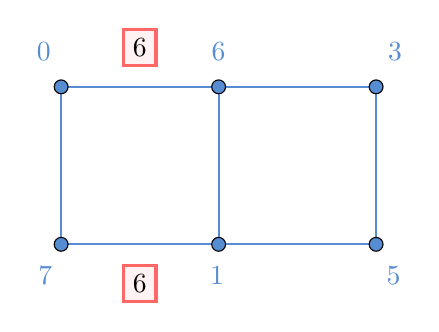
\begin{tikzpicture}
			\draw [cackithi,line width=0.8pt] (0.,2.)-- (4.,2.);
			\draw [cackithi,line width=0.8pt] (4.,2.)-- (4.,0.);
			\draw [cackithi,line width=0.8pt] (4.,0.)-- (0.,0.);
			\draw [cackithi,line width=0.8pt] (0.,0.)-- (0.,2.);
			\draw [cackithi,line width=0.8pt] (2.,2.)-- (2.,0.);
			
			\draw [fill=cackithi] (0.,2.) circle (2.5pt);
			\draw[color=cackithi] (-0.22,2.45) node {$0$};
			\draw [fill=cackithi] (4.,2.) circle (2.5pt);
			\draw[color=cackithi] (4.24,2.45) node {$3$};
			\draw [fill=cackithi] (4.,0.) circle (2.5pt);
			\draw[color=cackithi] (4.22,-0.4) node {$5$};
			\draw [fill=cackithi] (0.,0.) circle (2.5pt);
			\draw[color=cackithi] (-0.2,-0.4) node {$7$};
			\draw [fill=cackithi] (2.,2.) circle (2.5pt);
			\draw[color=cackithi] (2.,2.45) node {$6$};
			\draw [fill=cackithi] (2.,0.) circle (2.5pt);
			\draw[color=cackithi] (1.98,-0.4) node {$1$};
			\draw (1,2.5) node[squarednode] {$6$};
			\draw (1,-0.5) node[squarednode] {$6$};
		\end{tikzpicture}
		\vspace*{-5pt}
	\end{figure}
	Hình thứ hai cũng không phải là một dán nhãn duyên dáng bởi vì có hai nhãn $7$  bằng nhau. 
	\begin{figure}[H]
		\vspace*{-10pt}
		\centering
		\captionsetup{labelformat= empty, justification=centering}
		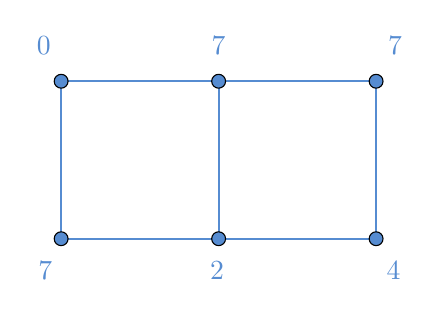
\begin{tikzpicture}
			\draw [cackithi, line width=0.8pt] (0.,2.)-- (4.,2.);
			\draw [cackithi,line width=0.8pt] (4.,2.)-- (4.,0.);
			\draw [cackithi,line width=0.8pt] (4.,0.)-- (0.,0.);
			\draw [cackithi,line width=0.8pt] (0.,0.)-- (0.,2.);
			\draw [cackithi,line width=0.8pt] (2.,2.)-- (2.,0.);
			
			\draw [fill=cackithi] (0.,2.) circle (2.5pt);
			\draw[color=cackithi] (-0.22,2.45) node {$0$};
			\draw [fill=cackithi] (4.,2.) circle (2.5pt);
			\draw[color=cackithi] (4.24,2.45) node {$7$};
			\draw [fill=cackithi] (4.,0.) circle (2.5pt);
			\draw[color=cackithi] (4.22,-0.4) node {$4$};
			\draw [fill=cackithi] (0.,0.) circle (2.5pt);
			\draw[color=cackithi] (-0.2,-0.4) node {$7$};
			\draw [fill=cackithi] (2.,2.) circle (2.5pt);
			\draw[color=cackithi] (2.,2.45) node {$7$};
			\draw [fill=cackithi] (2.,0.) circle (2.5pt);
			\draw[color=cackithi] (1.98,-0.4) node {$2$};
		\end{tikzpicture}
		\vspace*{-10pt}
	\end{figure}
	$2.$ Hình đã cho có thể được bổ sung như sau: 
	\begin{figure}[H]
		\vspace*{-10pt}
		\centering
		\captionsetup{labelformat= empty, justification=centering}
		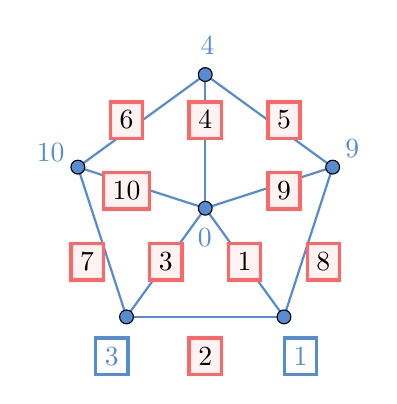
\begin{tikzpicture}
			\draw [cackithi,line width=0.8pt] (-1.6180339887498947,2.9021130325903073)-- (0.,2.38);
			\draw [cackithi,line width=0.8pt] (0.,2.38)-- (-1.,1.);
			\draw [cackithi,line width=0.8pt] (0.,2.38)-- (1.,1.);
			\draw [cackithi,line width=0.8pt] (0.,2.38)-- (1.618033988749895,2.9021130325903064);
			\draw [cackithi,line width=0.8pt] (0.,4.077683537175253)-- (0.,2.38);
			\draw [cackithi,line width=0.8pt] (0.,4.077683537175253)-- (-1.6180339887498947,2.9021130325903073);
			\draw [cackithi,line width=0.8pt] (-1.6180339887498947,2.9021130325903073)-- (-1.,1.);
			\draw [cackithi,line width=0.8pt] (-1.,1.)-- (1.,1.);
			\draw [cackithi,line width=0.8pt] (1.,1.)-- (1.618033988749895,2.9021130325903064);
			\draw [cackithi,line width=0.8pt] (1.618033988749895,2.9021130325903064)-- (0.,4.077683537175253);
			\draw [fill=cackithi] (-1.,1.) circle (2.5pt);
			\draw[color=cackithi] (-1.18624795654696,0.5) node[sqnode] {$3$};
			\draw (0,0.5) node[squarednode] {$2$};
			\draw (-1.5,1.7) node[squarednode] {$7$};
			\draw (-0.5,1.7) node[squarednode] {$3$};
			\draw (0.5,1.7) node[squarednode] {$1$};
			\draw (1.5,1.7) node[squarednode] {$8$};
			\draw (-1,3.5) node[squarednode] {$6$};
			\draw (-1,2.6) node[squarednode] {$10$};
			\draw (0,3.5) node[squarednode] {$4$};
			\draw (1,2.6) node[squarednode] {$9$};
			\draw (1,3.5) node[squarednode] {$5$};
			\draw [fill=cackithi] (1.,1.) circle (2.5pt);
			\draw[color=cackithi] (1.209997363286399,0.5) node[sqnode] {$1$};
			\draw [fill=cackithi] (1.618033988749895,2.9021130325903064) circle (2.5pt);
			\draw[color=cackithi] (1.8681210778885187,3.1434351104783014) node {$9$};
			\draw [fill=cackithi] (0.,4.077683537175253) circle (2.5pt);
			\draw[color=cackithi] (0.028749670410799504,4.4428075726414615) node {$4$};
			\draw [fill=cackithi] (-1.6180339887498947,2.9021130325903073) circle (2.5pt);
			\draw[color=cackithi] (-1.9624964404366394,3.0928102093550613) node {$10$};
			\draw [fill=cackithi] (0.,2.38) circle (2.5pt);
			\draw[color=cackithi] (-0.005000263671360479,2.012812318725942) node {$0$};
		\end{tikzpicture}
%		\vspace*{-5pt}
	\end{figure}
	\textbf{\color{cackithi}B. Trường hợp thẳng hàng}
	\vskip 0.05cm
	$1.$ Một dán nhãn duyên dáng của hình $L_5$	 

	\begin{figure}[H]
		\vspace*{-5pt}
		\centering
		\captionsetup{labelformat= empty, justification=centering}
		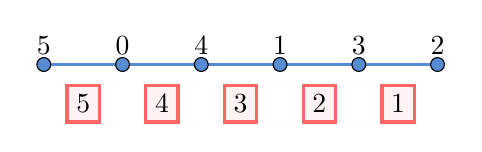
\begin{tikzpicture}
			\draw[cackithi, line width=0.8pt] (0,0) -- (5,0);
			\draw [fill=cackithi] (0,0) node[above]{$5$} circle (2.5pt);
			\draw [fill=cackithi] (1,0) node[above]{$0$} circle (2.5pt);
			\draw [fill=cackithi] (2,0) node[above]{$4$} circle (2.5pt);
			\draw [fill=cackithi] (3,0) node[above]{$1$} circle (2.5pt);
			\draw [fill=cackithi] (4,0) node[above]{$3$} circle (2.5pt);
			\draw [fill=cackithi] (5,0) node[above]{$2$} circle (2.5pt);
			
			
			\draw(0.5,-0.5) node[squarednode]{$5$};
			\draw(1.5,-0.5) node[squarednode]{$4$};
			\draw(2.5,-0.5) node[squarednode]{$3$};
			\draw(3.5,-0.5) node[squarednode]{$2$};
			\draw(4.5,-0.5) node[squarednode]{$1$};
		\end{tikzpicture}
		\vspace*{-10pt}
	\end{figure}
	Một dán nhãn duyên dáng của hình $L_6$	 

	\begin{figure}[H]
		\vspace*{-5pt}
		\centering
		\captionsetup{labelformat= empty, justification=centering}
		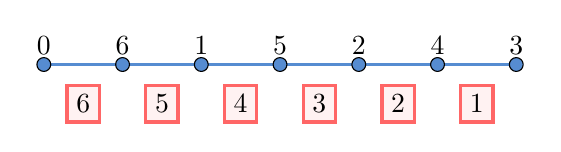
\begin{tikzpicture}
			\draw[cackithi, line width=0.8pt] (0,0) -- (6,0);
			\draw [fill=cackithi] (0,0) node[above]{$0$} circle (2.5pt);
			\draw [fill=cackithi] (1,0) node[above]{$6$} circle (2.5pt);
			\draw [fill=cackithi] (2,0) node[above]{$1$} circle (2.5pt);
			\draw [fill=cackithi] (3,0) node[above]{$5$} circle (2.5pt);
			\draw [fill=cackithi] (4,0) node[above]{$2$} circle (2.5pt);
			\draw [fill=cackithi] (5,0) node[above]{$4$} circle (2.5pt);
			\draw [fill=cackithi] (6,0) node[above]{$3$} circle (2.5pt);
			
			
			\draw(0.5,-0.5) node[squarednode]{$6$};
			\draw(1.5,-0.5) node[squarednode]{$5$};
			\draw(2.5,-0.5) node[squarednode]{$4$};
			\draw(3.5,-0.5) node[squarednode]{$3$};
			\draw(4.5,-0.5) node[squarednode]{$2$};
			\draw(5.5,-0.5) node[squarednode]{$1$};
		\end{tikzpicture}
		\vspace*{-10pt}
	\end{figure}
	Sự dán nhãn duyên dáng của hình $L_7$	 

	\begin{figure}[H]
		\vspace*{-5pt}
		\centering
		\captionsetup{labelformat= empty, justification=centering}
		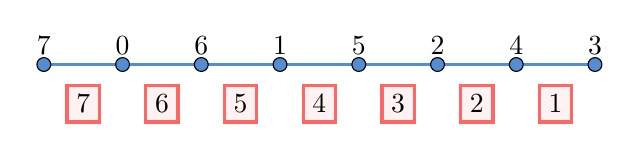
\begin{tikzpicture}
			\draw[cackithi, line width=0.8pt] (0,0) -- (7,0);
			\draw [fill=cackithi] (0,0) node[above]{$7$} circle (2.5pt);
			\draw [fill=cackithi] (1,0) node[above]{$0$} circle (2.5pt);
			\draw [fill=cackithi] (2,0) node[above]{$6$} circle (2.5pt);
			\draw [fill=cackithi] (3,0) node[above]{$1$} circle (2.5pt);
			\draw [fill=cackithi] (4,0) node[above]{$5$} circle (2.5pt);
			\draw [fill=cackithi] (5,0) node[above]{$2$} circle (2.5pt);
			\draw [fill=cackithi] (6,0) node[above]{$4$} circle (2.5pt);
			\draw [fill=cackithi] (7,0) node[above]{$3$} circle (2.5pt);
			
			
			\draw(0.5,-0.5) node[squarednode]{$7$};
			\draw(1.5,-0.5) node[squarednode]{$6$};
			\draw(2.5,-0.5) node[squarednode]{$5$};
			\draw(3.5,-0.5) node[squarednode]{$4$};
			\draw(4.5,-0.5) node[squarednode]{$3$};
			\draw(5.5,-0.5) node[squarednode]{$2$};
			\draw(6.5,-0.5) node[squarednode]{$1$};
		\end{tikzpicture}
		\vspace*{-10pt}
	\end{figure}
	$2.$ Tương tự như các dán nhãn của hình $L_4$ và $L_6$ phía trên, ta có thể dán nhãn hình $L_{2022}$ như sau: ta đánh số các điểm từ trái qua phải dựa vào dãy sau: 
	\begin{align*}
		&0,2022,1,2021,2,2020,3,2019,4,\\
		&2018 \ldots,1000,1012,1011
	\end{align*}
	Với cách dán nhãn trên, ta nhận được các trọng số từ trái qua phải là: $2022 ,$ $2021,$ $\ldots,4,3,2,1$. Đó là một dán nhãn duyên dáng của hình $L_{2022}$.
	\vskip 0.05cm 
	\textbf{\color{cackithi}C. Trường hợp đa giác}
	\vskip 0.05cm
	$1.$ Ta có thể dán nhãn tam giác và tứ giác một cách duyên dáng như sau: 
	\begin{figure}[H]
		\centering
		\vspace*{-5pt}
		\captionsetup{labelformat= empty, justification=centering}
		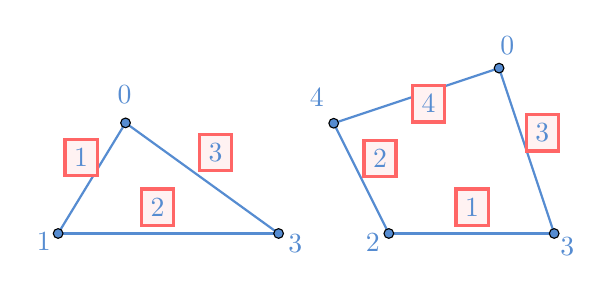
\begin{tikzpicture}[scale=0.7]
			\draw [cackithi, line width=0.8pt] (1.223091301970301,2.0066510197535226)-- (0,0);
			\draw [cackithi,line width=0.8pt] (0,0)-- (4,0);
			\draw [cackithi,line width=0.8pt] (4,0)-- (1.223091301970301,2.0066510197535226);
			\draw [cackithi,line width=0.8pt] (6,0)-- (5,2);
			\draw [cackithi,line width=0.8pt] (5,2)-- (8,3);
			\draw [cackithi,line width=0.8pt] (8,3)-- (9,0);
			\draw [cackithi,line width=0.8pt] (6,0)-- (9,0);

				\draw [fill=cackithi] (1.223091301970301,2.0066510197535226) circle (2.5pt);
				\draw[color=cackithi] (1.2043242804043022,2.522744112818487) node {$0$};
				\draw [fill=cackithi] (0,0) circle (2.5pt);
				\draw[color=cackithi] (-0.259503401743597,-0.14217294955332546) node {$1$};
				\draw[color=cackithi] (0.4161093746323564,1.3779557972925676) node[squarednode] {$1$};
				\draw [fill=cackithi] (4,0) circle (2.5pt);
				\draw[color=cackithi] (4.300882838794089,-0.17970699268532278) node {$3$};
				\draw[color=cackithi] (1.8048689705162608,0.4771387621246309) node[squarednode] {$2$};
				\draw[color=cackithi] (2.8558221782121884,1.4717909051225608) node[squarednode] {$3$};
				\draw [fill=cackithi] (6,0) circle (2.5pt);
				\draw[color=cackithi] (5.708409456243992,-0.16093997111932415) node {$2$};
				\draw [fill=cackithi] (5,2) circle (2.5pt);
				\draw[color=cackithi] (4.694990291680062,2.4664430481204906) node {$4$};
				\draw[color=cackithi] (5.839778607205983,1.3591887757265688) node[squarednode] {$2$};
				\draw [fill=cackithi] (8,3) circle (2.5pt);
				\draw[color=cackithi] (8.148122259823824,3.4047941264204247) node {$0$};
				\draw[color=cackithi] (6.721828620807923,2.3538409187244986) node[squarednode] {$4$};
				\draw [fill=cackithi] (9,0) circle (2.5pt);
				\draw[color=cackithi] (9.23660951065175,-0.23600805738331884) node {$3$};
				\draw[color=cackithi] (8.78620099306778,1.8283643148765356) node[squarednode] {$3$};
				\draw[color=cackithi] (7.510043526579868,0.4771387621246309) node[squarednode] {$1$};
		\end{tikzpicture}
		\vspace*{-10pt}
	\end{figure}
	$2.$ Bằng cách thêm đỉnh số $12$ như hình dưới vào một đa giác $11$ cạnh cho trước ta nhận được một dán nhãn duyên dáng của đa giác $12$ cạnh. 
	\begin{figure}[H]
		\centering
%		\vspace*{-5pt}
		\captionsetup{labelformat= empty, justification=centering}
		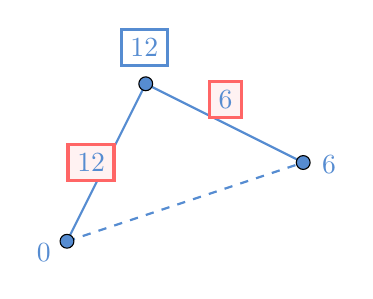
\begin{tikzpicture}
			\draw [cackithi, line width=0.8pt] (-3,3)-- (-4,1);
			\draw [cackithi,dashed, line width=0.8pt] (-4,1)-- (-1,2);
			\draw [cackithi,line width=0.8pt] (-3,3)-- (-1,2);
		
				\draw [fill=cackithi] (-3,3) circle (2.5pt);
				\draw[color=cackithi] (-3.018255571945407,3.4610951911184205) node[sqnode] {$12$};
				\draw [fill=cackithi] (-4,1) circle (2.5pt);
				\draw[color=cackithi] (-4.294413038433319,0.8524791934446044) node {$0$};
				\draw[color=cackithi] (-3.6938683483213604,2.0) node[squarednode] {$12$};
				\draw [fill=cackithi] (-1,2) circle (2.5pt);
				\draw[color=cackithi] (-0.6723778761955685,1.978500487404525) node {$6$};
				\draw[color=cackithi] (-1.986069385815478,2.8) node[squarednode] {$6$};
		\end{tikzpicture}
		\vspace*{-10pt}
	\end{figure}
	$3a.$ Nếu hai đỉnh kề nhau khác tính chẵn lẻ thì hiệu của chúng là một số lẻ, do đó trọng số là số lẻ. 
	\vskip 0.05cm
	$3b.$ Hoàn toàn tương tự như trên, nếu hai đỉnh kề nhau có cùng tính chẵn lẻ thì trọng số của đoạn thẳng nối hai đỉnh đó là một số chẵn.  
	\vskip 0.05cm
	$4.$ Giả sử phản chứng rằng tồn tại dán nhãn duyên dáng đối với hình ngũ giác. Khi đó trọng số các cạnh sẽ là các số tự nhiên từ $1$ tới $5$, trong đó có $3$ số lẻ và $2$ số chẵn. Đối với $3$ cạnh có trọng số lẻ thì các đỉnh liên kết phải khác tính chẵn lẻ, nếu không trọng số sẽ là số chẵn theo chứng minh trên. Ta có hai trường hợp sau:
	\vskip 0.05cm 
	Trường hợp ${1}$: $3$ cạnh trọng số lẻ kề nhau.
	\begin{figure}[H]
		\centering
		\vspace*{-5pt}
		\captionsetup{labelformat= empty, justification=centering}
		\begin{tikzpicture}[scale=0.75]
			\draw [line width=0.8pt,color=cackithi] (-1,0)-- (1,0);
			\draw [line width=0.8pt,color=cackithi] (1,0)-- (1.618033988749895,1.9021130325903064);
			\draw [line width=0.8pt,color=cackithi] (1.618033988749895,1.9021130325903064)-- (0,3.077683537175253);
			\draw [line width=0.8pt,color=cackithi] (0,3.077683537175253)-- (-1.6180339887498947,1.9021130325903073);
			\draw [line width=0.8pt,color=cackithi] (-1.6180339887498947,1.9021130325903073)-- (-1,0);
			\draw [line width=0.8pt,color=cackithi] (4,0)-- (6,0);
			\draw [line width=0.8pt,color=cackithi] (6,0)-- (6.618033988749895,1.9021130325903064);
			\draw [line width=0.8pt,color=cackithi] (6.618033988749895,1.9021130325903064)-- (5,3.077683537175253);
			\draw [line width=0.8pt,color=cackithi] (5,3.077683537175253)-- (3.381966011250105,1.9021130325903073);
			\draw [line width=0.8pt,color=cackithi] (3.381966011250105,1.9021130325903073)-- (4,0);
		
				\draw [fill=cackithi] (-1,0) circle (2.5pt);
				\draw[color=cackithi] (-1.291689587873526,-0.6) node[squarednode] {L};
				\draw(0,0)node[below] {Chẵn};
				\draw [fill=cackithi] (1,0) circle (2.5pt);
				\draw[color=cackithi] (1.2418583235362997,-0.6) node[squarednode] {L};
				\draw(1.5,1)node[below] {Lẻ};
				\draw [fill=cackithi] (1.618033988749895,1.9021130325903064) circle (2.5pt);
				\draw[color=cackithi] (1.9,1.3) node[squarednode] {C};
				\draw(1,3)node[below] {Lẻ};
				\draw [fill=cackithi] (0,3.077683537175253) circle (2.5pt);
				\draw[color=cackithi] (0.022001921746383594,3.7) node[squarednode] {L};
				\draw(-1,3)node[below] {Lẻ};
				\draw [fill=cackithi] (-1.6180339887498947,1.9021130325903073) circle (2.5pt);
				\draw[color=cackithi] (-1.929768321117482,2.5) node[squarednode] {C};
				\draw(-1.3,1)node[below] {Chẵn};
				\draw [fill=cackithi] (4,0) circle (2.5pt);
				\draw[color=cackithi] (3.85047432121012,-0.6) node[squarednode] {C};
				\draw(5,0)node[below] {Chẵn};
				\draw(6.6,0.9)node[below] {Lẻ};
				\draw(6,3)node[below] {Lẻ};
				\draw(4,3)node[below] {Lẻ};
				\draw(3,1)node[below] {Chẵn};
				\draw [fill=cackithi] (6,0) circle (2.5pt);
				\draw[color=cackithi] (6.140050952261962,-0.6) node[squarednode] {C};
				\draw [fill=cackithi] (6.618033988749895,1.9021130325903064) circle (2.5pt);
				\draw[color=cackithi] (6.909498836467909,1.2224717677625083) node[squarednode] {L};
				\draw [fill=cackithi] (5,3.077683537175253) circle (2.5pt);
				\draw[color=cackithi] (5.032796679868039,3.7) node[squarednode] {C};
				\draw [fill=cackithi] (3.381966011250105,1.9021130325903073) circle (2.5pt);
				\draw[color=cackithi] (3.081026437004173,2.5) node[squarednode] {L};
		\end{tikzpicture}
		\vspace*{-10pt}
	\end{figure}
	Trường hợp ${2}$: $2$ cạnh trọng số lẻ kề nhau liền kề với một cạnh có trọng số chẵn. 
	\begin{figure}[H]
		\centering
		\vspace*{-5pt}
		\captionsetup{labelformat= empty, justification=centering}
		\begin{tikzpicture}[scale=0.75]
			\draw [line width=0.8pt,color=cackithi] (-1,0)-- (1,0);
			\draw [line width=0.8pt,color=cackithi] (1,0)-- (1.618033988749895,1.9021130325903064);
			\draw [line width=0.8pt,color=cackithi] (1.618033988749895,1.9021130325903064)-- (0,3.077683537175253);
			\draw [line width=0.8pt,color=cackithi] (0,3.077683537175253)-- (-1.6180339887498947,1.9021130325903073);
			\draw [line width=0.8pt,color=cackithi] (-1.6180339887498947,1.9021130325903073)-- (-1,0);
			\draw [line width=0.8pt,color=cackithi] (4,0)-- (6,0);
			\draw [line width=0.8pt,color=cackithi] (6,0)-- (6.618033988749895,1.9021130325903064);
			\draw [line width=0.8pt,color=cackithi] (6.618033988749895,1.9021130325903064)-- (5,3.077683537175253);
			\draw [line width=0.8pt,color=cackithi] (5,3.077683537175253)-- (3.381966011250105,1.9021130325903073);
			\draw [line width=0.8pt,color=cackithi] (3.381966011250105,1.9021130325903073)-- (4,0);
			
			\draw [fill=cackithi] (-1,0) circle (2.5pt);
			\draw[color=cackithi] (-1.291689587873526,-0.6) node[squarednode] {C};
			\draw(0,0)node[below] {Lẻ};
			\draw [fill=cackithi] (1,0) circle (2.5pt);
			\draw[color=cackithi] (1.2418583235362997,-0.6) node[squarednode] {L};
			\draw(1.5,1)node[below] {Chẵn};
			\draw [fill=cackithi] (1.618033988749895,1.9021130325903064) circle (2.5pt);
			\draw[color=cackithi] (1.9,1.3) node[squarednode] {L};
			\draw(1,3)node[below] {Lẻ};
			\draw [fill=cackithi] (0,3.077683537175253) circle (2.5pt);
			\draw[color=cackithi] (0.022001921746383594,3.7) node[squarednode] {C};
			\draw(-1,3)node[below] {Lẻ};
			\draw [fill=cackithi] (-1.6180339887498947,1.9021130325903073) circle (2.5pt);
			\draw[color=cackithi] (-1.929768321117482,2.5) node[squarednode] {L};
			\draw(-1.3,1)node[below] {Chẵn};
			\draw [fill=cackithi] (4,0) circle (2.5pt);
			\draw[color=cackithi] (3.85047432121012,-0.6) node[squarednode] {L};
			\draw(5,0)node[below] {Lẻ};
			\draw(6.6,0.9)node[below] {Chẵn};
			\draw(6,3)node[below] {Lẻ};
			\draw(4,3)node[below] {Lẻ};
			\draw(3,1)node[below] {Chẵn};
			\draw [fill=cackithi] (6,0) circle (2.5pt);
			\draw[color=cackithi] (6.140050952261962,-0.6) node[squarednode] {C};
			\draw [fill=cackithi] (6.618033988749895,1.9021130325903064) circle (2.5pt);
			\draw[color=cackithi] (6.909498836467909,1.2224717677625083) node[squarednode] {C};
			\draw [fill=cackithi] (5,3.077683537175253) circle (2.5pt);
			\draw[color=cackithi] (5.032796679868039,3.7) node[squarednode] {L};
			\draw [fill=cackithi] (3.381966011250105,1.9021130325903073) circle (2.5pt);
			\draw[color=cackithi] (3.081026437004173,2.5) node[squarednode] {C};
		\end{tikzpicture}
		\vspace*{-10pt}
	\end{figure}
	Khi đó sẽ tồn tại hai đỉnh được dán nhãn khác tính chẵn lẻ nhưng lại cho trọng số là số chẵn như minh họa phía trên. Điều này mâu thuẫn với tính chất đã chứng minh ở phần trước. Do vậy, không tồn tại bất cứ dán nhãn duyên dáng cho hình ngũ giác.
	\vskip 0.05cm 
	\textbf{\color{cackithi}D. Một hình đa giác với số cạnh lớn}
	\vskip 0.05cm
	$1.$ Số các đoạn thẳng bằng số cách chọn ra $2$ điểm từ $2021$ điểm, nghĩa là 
	$\dfrac{1}{2}\times 2022\times 2021=2 043 231$. Vậy, hình $K_{2022}$ được tạo thành từ $2043231$ đoạn thẳng. 
	\vskip 0.05cm
	$2a.$ Số đoạn thẳng mang trọng số lẻ chính là số những số tự nhiên lẻ của tập hợp $\{1,2,...,2043231\}$, nghĩa là bằng  $1021616$.
	\vskip 0.05cm 
	$2b.$ Vì có $p$ điểm được dán nhãn là số chẵn nên số điểm được dán nhãn là số lẻ là $2022-p$. Số những đoạn thẳng có trọng số lẻ chính là số cặp điểm được dán nhãn khác nhau về tính chẵn lẻ, do đó có tất cả  $p(2022-p)$ đoạn.
	\vskip 0.05cm
	$3.$ Giả sử hình  $K_{2022}$ có một dán nhãn duyên dáng. Khi đó có $1 021 616$ đoạn thẳng mang trọng số lẻ. Suy ra tồn tại một số tự nhiên $p$ sao cho: $p(2022-p)=1 021 616$, nghĩa là $p^2-2022p+1 021 616=0$. Phương trình này không có nghiệm nguyên, mâu thuẫn. 
	\vskip 0.05cm
	\textbf{\color{cackithi}Bài $\pmb{2}$ ( Dành cho thí sinh theo chương trình chuyên)} 
	\vskip 0.05cm
	\textbf{\color{cackithi}Phần A}
	\vskip 0.05cm
	$1a$. Các số $21$ và $136$ là phân chia được đơn nguyên vì: $21=1+2+3+4+5+6$ và $136=1+2+3+4+5+6+7+8+9+10+11+12+13+14+15+16$.
	\vskip 0.05cm 
	$1b.$ Nếu $1850$ là phân chia được đơn nguyên thì tồn tại số tự nhiên $n$ sao cho: 
	\begin{align*}
		1+2+3+\cdots+n=1850.
	\end{align*}
	Suy ra 
	\begin{align*}
		\frac{n(n+1)}{2} = 1850.
	\end{align*}
	Hay, $n^2+n-3700=0$. Phương trình bậc hai này không có nghiệm nguyên, mâu thuẫn. Do đó $1850$ không phải là số phân chia được đơn nguyên. 
	\vskip 0.05cm
	$2.$ Số tự nhiên $a$ lớn hơn hoặc bằng $3$ là một số phân chia được đơn nguyên khi và chỉ khi phương trình: $n^2+n-2a=0$ có ít nhất một nghiệm nguyên dương. Điều đó có nghĩa là biệt thức $\Delta=1+8a$ là một số chính phương và ít nhất một trong hai nghiệm \linebreak$x_1=\dfrac{-1-\sqrt{1+ 8a}}{2}$ và $x_2=\dfrac{-1+\sqrt{1+ 8a}}{2}$ là nguyên dương. Từ đó ta suy ra rằng điều kiện cần và đủ để $a$ là số phân chia được đơn nguyên là $1+8a$ là một số chính phương.
	\vskip 0.05cm  
	\textbf{\color{cackithi}Phần B}
	\vskip 0.05cm
	$1.$ Các số $9$ và $15$ là phân chia được vì $9=4+5$ và $15=7+8=4+5+6=1+2+3+4+5$. Tuy nhiên số $16$ thì không phân chia được vì:
	\begin{align*}
		&1\!+\!2\!+\!3\!+\!4\!+\!5\!<\!16\!<\!1\!+\!2\!+\!3\!+\!4\!+\!5\!+\!6;\\
		&2+3+4+5<16<2+3+4+5+6;\\
		&3+4+5<16<3+4+5+6;\\
		&4+5+6<16<4+5+6+7;\\
		&5\!+\!6\!<\!16\!<\!5\!+\!6\!+\!7; 6\!+\!7\!<\!16\!<\!6\!+\!7\!+\!8;\\
		&7+8<16<7+8+9 \text{ và } 8+9>16.
	\end{align*}
	$2.$ Gọi $n$ là số tự nhiên là lẻ và lớn hơn hoặc bằng $3$. Đặt $n=2k+1$. Khi đó $n=k+(k+1)$ do đó là phân chia được.
	\vskip 0.05cm  
	$3.$ $S=(q+1)+(q+2)+\cdots+(q+k)=(q+q+\cdots+q)+(1+2+\cdots+k)=kq+\dfrac{k(k+1)}{2}$.
	\vskip 0.05cm
	Từ đó suy ra: $2S=2kq+k(k+1)=k(2q+k+1)$. 
	\vskip 0.05cm
	$4.$ Giả sử $N=2^p$ là một lũy thừa của $2$ và là phân chia được. Theo kết câu trên, tồn tại các số tự nhiên $k$ và $q$ lớn hơn hoặc bằng $2$ sao cho: $2N=k(2q+k+1)$. Điều này là vô lý vì vế trái là một luỹ thừa của $2$ còn vế phải là tích của một số chẵn và một số lẻ lớn hơn $1$. 
	\vskip 0.05cm
	$5a.$ Ta có $56=2^3\times7$ nên $r=3$ và $m=7$. Hơn nữa $2\times 56=2^4\times7=7(2\times4+7+1)$. Do đó $56$ được viết dưới dạng tổng được định nghĩa ở ý $3)$ phần $B)$ với $k=7$ và $q=4$. Cụ thể hơn $56=5+6+7+8+9+10+11$, từ đó suy ra $56$ là số tự nhiên phân chia được. 
	\vskip 0.05cm
	$5b.$ Tương tự như trên $2\times 44=8\times11=8(2\times1+8+1)$. Do đó $44=2+3+4+5+6+7+8+9$. Ta kết luận rằng $44$ là số tự nhiên phân chia được.
	\vskip 0.05cm 
	$5c.$ Gọi $n$ là một số tự nhiên dương chẵn và không phải là lũy thừa của $2$. Đặt $n=2^r\times m$, với $m$ là một số nguyên lẻ lớn hơn hoặc bằng $3$ và $r$ một số nguyên dương. Ta suy ra $2n=2^{r+1}\times m$. Ta xét hai trường hợp sau. 
	\vskip 0.05cm
	Trường hợp $1$: Nếu $m>2^{r+1}$, tức là $m \ge 2^{r+1}+1$ và vì $m$ là một số tự nhiên lẻ nên ta suy ra tồn tại một số tự nhiên $l\ge 0$ sao cho $m=2^{r+1}+1+2l$. Khi đó $2n=2^{r+1}(2l+2^{r+1}+1)$. Do đó $n$ được viết dưới dạng tổng được định nghĩa ở ý $3)$ phần $B)$ với $k=2^{r+1}$ và $q=l$. Hay nói cách khác $n$ là số tự nhiên phân chia được. 
	\vskip 0.05cm
	Trường hợp $2$: Nếu $m<2^{r+1}$ tức là $m+1 \le 2^{r+1}$ và vì $2^{r+1}$ là một số tự nhiên chẵn nên ta suy ra tồn tại một số tự nhiên $l \ge 0$ sao cho $2^{r+1}=m+1+2l$. Khi đó $2n=m(2l+m+1)$. Do đó $n$ được viết dưới dạng tổng được định nghĩa ở ý $3)$ phần $B)$ với $k=m$ và $q=l$. Ta kết luận rằng n là số tự nhiên phân chia được.  
	\vskip 0.05cm
	Lưu ý rằng trường hợp $m=2^{r+1}$ không thể xảy ra vì $m$ là số lẻ. 
	\vskip 0.05cm
	$6.$ Từ những kết quả nhận được ở câu hỏi $2)$ và câu hỏi $5)$ ta suy ra rằng tập hợp những số tự nhiên phân chia được gồm những số tự nhiên lẻ lớn hơn hoặc bằng $3$ và những số tự nhiên chẵn không  viết được dưới dạng lũy thừa của $2$. 
	\vskip 0.05cm
	\textbf{\color{cackithi}Phần C}
	\vskip 0.05cm
	$1.$ $13$ là số tự nhiên lẻ lớn hơn $3$, nên theo kết quả trên $13$ là số tự nhiên phân chia được, hơn nữa $2\times 13=2(2\times 5+2+1)$ nên $13$ được viết dưới dạng tổng được định nghĩa ở ý $3)$ phần $B)$ với $k=2$ và $q=5$. Tức là $13=(5+1)+(5+2)$. Giả sử tồn tại một biểu diễn khác của $13$, ta suy ra tồn tại những số tự nhiên $k'\ ge 2$ và $q'$ sao cho $13=(q'+1)+(q'+2)+\cdots+(q'+k')$. Theo kết quả phần $B)$, ta có $2\times 13=k'(2q'+k'+1)$. Vì $2q'+k'+1>k'$ nên ta suy ra $k'<13$. Vì $13$ là số nguyên tố, nên ta suy ra $k'\ge 2$ là ước của $2$. Hay nói cách khác $k'=2=k$. Thay vào đẳng thức ta được $q'=5=q$. Do đó $13$ là số tự nhiên phân chia được một cách duy nhất. Tương tự $25$ là số tự nhiên phân chia được, tuy nhiên $2\times25=2\times(2\times11+2+1)=5(2\times2+5+1)$, nên theo kết quả ở phần $B)$, số tự nhiên $25$ có thể được biểu diễn dưới dạng tổng theo $2$ cách $25=12+13$ và $25=3+4+5+6+7$ nên nó không phải là số tự nhiên phân chia được một cách duy nhất.
	\vskip 0.05cm 
	$2a.$ Ta có $n=(q+1)+(q+2)+\cdots+(q+k)=k\times q+\dfrac{k(k+1)}{2}$. Nếu $k$ là số tự nhiên chẵn thì $\dfrac{k}{2}$ là một số tự nhiên, do đó $n=\dfrac{k}{2}(2q+k+1)$. Nếu $k$ là một số tự nhiên lẻ thì $\dfrac{k}{2}$ là một số tự nhiên, do đó $n=k(q+\dfrac{k+1}{2})$. Từ đó ta kết luận rằng $n$ không phải là số nguyên tố.
	\vskip 0.05cm 
	$2b$. Gọi $p$ là tố lớn hơn hoặc bằng $3$, vì $p$ là số lẻ nên theo kết quả phần $B)$ $p$ là số tự nhiên phân chia được. Hơn nữa $p=(q+1)+(q+2)$ với $q=\dfrac{p-3}{2}$. Để  ý rằng $q$ là một số tự nhiên vì $p$ là một số lẻ lớn hơn hoặc bằng $3$. Ta sẽ chứng minh biểu diễn này là duy nhất. Tương tự câu $1)$ giả sử tồn tại một biểu diễn khác của $13$, ta suy ra tồn tại những số tự nhiên $k'\ge 2$ và $q'$ sao cho $p=(q'+1)+(q'+2)+\cdots+(q'+k')$. Theo kết quả phần $B)$, ta có $2\times p=k'(2q'+k'+1)$. Vì $2q'+k'+1>k'$ nên ta suy ra $k'<p$. Vì $p$ là số nguyên tố, nên ta suy ra $k'$ là ước của $2$. Hay nói cách khác $k'=2$. Thay vào đẳng thức ta được $q'=q$. Ta kết luận rằng mọi số nguyên tố lớn hơn hoặc bằng $3$ đều phân chia được một cách duy nhất. 
	\vskip 0.05cm
	\textbf{\color{cackithi}Bài $\pmb{3}$ (Dành cho các thí sinh không theo chương trình chuyên)} 
	\vskip 0.05cm
		\textbf{\color{cackithi}Số ba}
	\vskip 0.05cm
	$1.$ Dựa vào những sơ đồ dưới đây, ta có thể khẳng định rằng cả các số tự nhiên từ $1$ đến $12$ đều có thể đạt được bằng quy tắc nêu trên. 
	\[\begin{tikzcd}[column sep = 1.35em]
		4 \arrow{r}{:\ 2}  & 2 \arrow{r}{:\ 2}& 1, &4 \arrow{r}{:\ 2}  & 2,\\[-3ex]
		4 \arrow{r}{:\ 2}  & 2 \arrow{r}{\times 3}& 6  \arrow{r}{:\  2} & 3, & 4,\\[-3ex]
		4 \arrow{r}{:\ 2}  & 2 \arrow{r}{:\ 2} &1 \arrow{r}{\times 3}& 3  \arrow{r}{+2} & 5,\\[-3ex]
		4 \arrow{r}{:\ 2}  & 2 \arrow{r}{\times 3}& 6,\\[-3ex]
		4 \arrow{r}{\times  3}  & 12 \arrow{r}{+ 2}& 14\arrow{r}{: \ 2 }& 7,\\[-3ex]
		4 \arrow{r}{:\  2}  & 2 \arrow{r}{\times 3}& 6 \arrow{r}{+2 }& 8, \\[-3ex]
		4 \arrow{r}{:\ 2}  & 2 \arrow{r}{:\ 2} &1 \arrow{r}{\times 3}& 3  \arrow{r}{\times 3} & 9, \\[-3ex]
		4 \arrow{r}{:\ 2}  & 2 \arrow{r}{\times 3} &6 \arrow{r}{\times 3}& 18  \arrow{r}{+ 2} & 20 \arrow{r}{:\ 2} & 10,\\[-3ex]
		4 \arrow{r}{:\ 2}  & 2 \arrow{r}{:\ 2} &1 \arrow{r}{\times 3}& 3  \arrow{r}{\times 3} & 9 \arrow{r}{+ 2} & 11,\\[-3ex]
		4  \arrow{r}{\times 3} &12.
	\end{tikzcd}\]
	$2.$ Dựa vào kết quả trên, ta có thể thực hiện các phép toán sao cho kết quả là $8$. Sau đó ta tiếp tục áp dụng liên tiếp các phép toán sau:
	 \[
	 \begin{tikzcd}[column sep = 1.35em]
	 	8 \arrow{r}{\times 3} & 24\arrow{r}{\times 3} & 72 \arrow{r}{+ 2} & 74 \arrow{r}{\times 3}& 222\\[-3ex]
	 	222 \arrow{r}{+ 2} & 224 \arrow{r}{\times 3} & 672 \arrow{r}{+ 2} & 674 \arrow{r}{\times 3} & 2022.
	 \end{tikzcd}
	 \]
	Ta kết luận rằng $2022$ là số tự nhiên có thể đạt được theo các quy tắc đã nêu. 
	
	$3a$. Giả sử phản chứng rằng $m$ là bội của $3$. Đặt $m=3a$. Do $m$ là số không đạt được nhỏ nhất. nhỏ nhất nên $a$ là số đạt được. Thế nhưng khi đó, ta chỉ cần áp dụng thêm phép toán Nhân $3$  với kết quả $a$ để đạt được $m$. Hay nói cách khác $m$ là số tự nhiên đạt được, mâu thuẫn. Chứng tỏ rằng giả sử phản chứng là sai, nói cách khác $m$ không phải là bội của $3$.
	\vskip 0.05cm 
	$3b$. Giả sử $m-2$ là bội của $3$, đặt $m=3b+2$. Do $m$ là số không đạt được nhỏ nhất nên $b$ là đạt được. Khi đó, chỉ cần áp dụng thêm $2$ phép toán liên tiếp Nhân $3$  rồi Cộng $2$ với từ $b$ ta thu được $m$. Hay nói cách khác $m$ là số tự nhiên đạt được, mâu thuẫn. Vậy $m-2$ không phải là bội của $3$. 
	\vskip 0.05cm
	$3c.$ Nếu $m-1$ là bội của $3$, thì tồn tại số tự nhiên dương $c$ sao cho $m=3c+1>c$. Ta suy ra $2m=3\times 2c+2$. Nếu $2c$ là số tự nhiên không đạt được bằng cách áp dụng các quy tắc như trên, thì vì $m$ là nhỏ nhất trong những số không thể đạt được nên $m\ le 2c$, hay $3c+1 \le 2c \Leftrightarrow +1 \le 0$. Điều này mâu thuẫn với điều kiện $c$ là số tự nhiên. Ngược lại, nếu $2c$ là số tự nhiên đạt được, ta áp dụng thêm $3$ phép toán liên tiếp  Nhân $3$  rồi Cộng $2$  rồi  Chia $2$ với kết quả $2c$ ta thu được $m$. Hay nói cách khác $m$ cũng là số tự nhiên đạt được. Điều này mâu thuẫn với định nghĩa của $m$. Chứng tỏ rằng $m-1$ không phải là bội của $3$.
	\vskip 0.05cm
	$3d.$ Vì trong ba số tự nhiên liên tiếp luôn có một số là bội của $3$. Nên dựa vào những kết quả trên, nếu tồn tại những số tự nhiên không đạt được bằng cách áp dụng các quy tắc đã nêu với $m$ là số tự nhiên nhỏ nhất trong số chúng, khi đó $m-2,m-1$ và $m$ đều không phải là bội của $3$. Điều này mâu thuẫn với tính chất đã nêu. Chứng tỏ, mọi số tự nhiên dương đều đạt được bằng cách áp dụng các quy tắc đã nêu. 
	\vskip 0.05cm
	\textbf{\color{cackithi}\color{cackithi}Tài liệu tham khảo}
	\vskip 0.05cm
	[$1$] Les Olympiades nationales de mathématiques | Ministère de l'Education Nationale et de la Jeunesse
	\vskip 0.05cm
	[$2$] https://www.freemaths.fr/annales-olym\\piades-mathematiques-premieres-scientifiqu\\es-s/nationales/2022
\end{multicols}
\vspace*{-10pt}
\rule{1\linewidth}{0.1pt}
\begin{center}
	\textbf{\LARGE\color{cackithi}LỜI GIẢI, ĐÁP ÁN}
\end{center}
\begin{multicols}{2}
	Sau đó, hai máy bay có đầy bình tiếp tục hành trình của mình còn chiếc còn $1/2$ bình quay trở lại sân bay ban đầu. 
	\vskip 0.05cm
	Sau khi tiếp tục đi được $1/8$ vòng Trái Đất, nghĩa là được $1/4$ vòng kể từ điểm xuất phát, chiếc còn lại chuyển $1/4$ bình nhiên liệu cho Pi. Khi này Pi có đầy bình và chiếc còn lại có $1/4$ bình, vừa đủ để quay trở lại. Bây giờ, Pi tiếp tục hành trình của mình còn chiếc máy bay kia quay trở lại sân bay ban đầu. Với đầy bình, Pi có thể đi được $3/4$ vòng Trái Đất kể từ điểm xuất phát. 
	\vskip 0.05cm
	Máy bay đầu tiên, với đầy bình bay theo hướng ngược lại (so với hướng ban đầu) để gặp máy bay của Pi ở vị trí $3/4$ vòng Trái Đất, khi đó máy bay đầu tiên còn $1/2$ bình sẽ tiếp cho máy bay của Pi $1/4$ bình, sao cho cả hai máy bay có $1/4$ bình, đủ để đi đến vị trí $7/8$ vòng Trái Đất. Khi hai chiếc máy bay này gặp nhau, chiếc còn lại bắt đầu xuất phát từ sân bay ban đầu với đầy bình và bay theo hướng ngược lại để gặp máy bay của Pi và chiếc thứ hai ở vị trí $7/8$ vòng Trái Đất và tiếp cho mỗi chiếc $1/4$ bình. Khi này, mỗi chiếc có đúng $1/4$ bình, vừa đủ để bay về sân bay ban đầu.   
	\vskip 0.05cm
	\textbf{\color{cackithi}Góc cờ}
	\vskip 0.05cm
	\textbf{\color{cackithi}Bài $\pmb{1}$.
				$\pmb{1}$.Vd$\pmb{4}$ Vb$\pmb{4}$ $\pmb{2}$.Xg$\pmb{2}$ Mh$\pmb{3}$} [$2$...Md$1$ $3$.Xd$2$]
	\vskip 0.05cm
	\textbf{\color{cackithi}$\pmb{3}$.Ke$\pmb{3}$} Mã đen bị bắt.
	\vskip 0.05cm
	\textbf{\color{cackithi}Bài $\pmb{2}$. 
				$\pmb{1}$.Vc$\pmb{4}$ Vc$\pmb{6}$} [$1$...Mh$3$ $2$.Xg$4$ Mf$2$ $3$.Xh$4$]
	\vskip 0.05cm
	\textbf{\color{cackithi}$\pmb{2}$.Xh$\pmb{4}$ Vd$\pmb{6}$ $\pmb{3}$.Vd$\pmb{4}$ Ve$\pmb{6}$ $\pmb{4}$.Ve$\pmb{3}$ Md$\pmb{1+}$ $\pmb{5}$.Vd$\pmb{2}$ Mb$\pmb{2}$} [$5$...Mf$2$ $6$.Ve$2$]
	\vskip 0.05cm
	\textbf{\color{cackithi}$\pmb{6}$.Xb$\pmb{4}$}
	\vskip 0.05cm
	\textbf{\color{cackithi}Bài $\pmb{3}$.
				$\pmb{1}$.Xd$\pmb{4}$!! Mb$\pmb{6}$} [$1$...Mb$2$ $2$.Ve$3$ Vf$5$ $3$.Vd$2$ Ve$5$ $4$.Xb$4$]
	\vskip 0.05cm
	\textbf{\color{cackithi}$\pmb{2}$.Ve$\pmb{5}$ Mc$\pmb{8}$ $\pmb{3}$.Ve$\pmb{6}$ Ma$\pmb{7}$ $\pmb{4}$.Vd$\pmb{7}$ Mb$\pmb{5}$} [$4$...Vf$5$ $5$.Xa$4$ Mb$5$ $6$.Xa$5$; $4$...Vg$6$ $5$.Xd$5$]
	\vskip 0.05cm
	\textbf{\color{cackithi}$\pmb{5}$.Xd$\pmb{5+}$}
	\vskip 0.05cm
	$\pmb{1-0}$
\end{multicols}
%\newpage
%\begingroup
%\AddToShipoutPicture*{\put(148,700){\includegraphics[scale=1]{../tieude1.pdf}}} 
%\centering
%\endgroup
%\vspace*{5pt}
%
%\begin{multicols}{2}
%	\setlength{\abovedisplayskip}{4pt}
%	\setlength{\belowdisplayskip}{4pt}
%	Trong phần đầu chuyên mục, chúng tôi sẽ trình bày lời giải của các bài toán trong cuộc thi Olympic toán Maclaurin năm $2021$ tại Vương quốc Anh đăng trong số báo $4/2022$. 
%	\begin{figure}[H]
%		\vspace*{-5pt}
%		\centering
%		\captionsetup{labelformat= empty, justification=centering}
%		\includegraphics[width= 0.85\linewidth]{gocolympic}
%		\vspace*{-5pt}
%	\end{figure}
%	{\bf\color{cackithi} OC$\pmb{7.}$} Cho tam giác $ABC$ như trong hình vẽ. Một đường tròn, đi qua điểm $C$ và tiếp xúc với $AB$ tại $B,$ cắt đường thẳng $AC$ tại $P$. Đường tròn thứ hai, đi qua điểm $B$ và tiếp xúc với $AC$ tại $C,$ cắt đường thẳng $AB$ tại $Q.$  Chứng minh rằng 
%	\begin{align*}
%		\frac{AP}{AQ}= \left(\frac{AB}{AC} \right)^3.
%	\end{align*}
%	\begin{figure}[H]
%		\vspace*{-5pt}
%		\centering
%		\includegraphics[width=0.8\linewidth]{OC7}
%		\vspace*{-5pt}
%	\end{figure}
%	\textit{Lời giải.} Ta nối $PB$ và $QC$ và khai thác tính chất: góc tạo bởi tiếp tuyến và dây cung bằng  góc nội tiếp chắn cung đó. Ta nhận được $ \angle BPC = \angle ABC = \angle QCA.$
%	\vskip 0.1cm
%	Như vậy các tam giác $ACQ, ABC$ and $APB$ đồng dạng vì có hai góc bằng nhau. Do đó
%	\begin{align*}
%		\frac{AQ}{AC}=\frac{AC}{AB}=\frac{AB}{AP}.
%	\end{align*}
%	Từ đây, ta nhận được $AP=\frac{AB^2}{AC}$
%	và $AQ=\frac{AC^2}{AB}$ và suy ra đẳng thức cần chứng minh. 
%	\vskip 0.1cm
%	{\bf\color{cackithi} OC$\pmb{8.}$} Một dãy số nguyên $a_1, a_2, a_3, \cdots$ được xác định bởi: 
%	\begin{align*}
%		&a_1 = k, a_{n + 1} = a_n +8n \\
%		 &\text{với mọi số nguyên}\ n \ge 1.
%	\end{align*}
%	Tìm tất cả các giá trị của $k$ sao cho mọi số hạng trong dãy đều là số chính phương.
%	\vskip 0.1cm
%	\textit{Lời giải.} 
%	Từ giả thiết ta có $a_1=k$ và $a_2=k+8$ là các số chính phương, giả sử $k=m^2$. Do chênh lệch giữa 2 số chính phương $(m+3)^2$ và $m^2$ là $(m+3)^2-m^2= m^2+6m+9-m^2=6m+9>8$ nên $k+8$ chỉ có thể bằng $(m+1)^2$ hoặc $(m+2)^2$. Tuy nhiên, nếu $k+8=(m+1)^2$ thì vô lý vì khi đó $8=(m+1)^2-m^2=2m+1$ là số lẻ. 
%	\vskip 0.1cm
%	Như vậy, chỉ còn lại khả năng duy nhất là $k+8=(m+2)^2.$ Ta suy ra $8=(m+2)^2-m^2=4m+4,$ tức là $m=1$, hay $k=1.$
%	\vskip 0.1cm
%	Ta kiểm tra lại rằng $k=1$ thỏa mãn đầu bài. Thật vậy, khi đó, ta dễ dàng tính được
%	$a_n=1+ 8(1+2\cdots (n-1))= 1+ 4n(n-1)=(2n-1)^2,$ luôn là số chính phương.   
%	\vskip 0.1cm
%	Như vậy $k=1$ là giá trị duy nhất thỏa mãn đầu bài.
%	\vskip 0.1cm
%	{\bf\color{cackithi} OC$\pmb{9.}$} Một con mèo và một con chuột lần lượt ở tại các ô trên cùng bên phải và dưới cùng bên trái của một bảng ô vuông kích thước $m\times n$, trong đó $m, n > 1.$ Mỗi giây cả hai đều di chuyển
%	chéo một ô (sang một trong các ô có chung đúng $1$ đỉnh với ô hiện tại).
%	\vskip 0.1cm
%	Với những cặp $(m, n)$ nào thì mèo và chuột có thể đồng thời đi đến cùng một ô?
%	\begin{center}
%		\begin{tikzpicture}
%			\draw[cackithi] (0,0) grid (7,4);
%			\node[inner sep=0pt] (mouse) at (0.5,0.5)
%			{\includegraphics[width=.06\textwidth]{mouse2.png}};
%			\node[inner sep=0pt] (mouse) at (6.5,3.5)
%			{\includegraphics[width=.04\textwidth]{cat1.png}};
%		\end{tikzpicture}
%	\end{center}
%	\textit{Lời giải.} Ta tô màu các ô vuông đen, trắng như bàn cờ vua.    
%	\begin{figure}[H]
%		\vspace*{-5pt}
%		\centering
%		\captionsetup{labelformat= empty, justification=centering}
%		\begin{tikzpicture}
%			\draw (0,0) grid (7,4);
%			\foreach \x in {0,2,4,6}{
%				 \foreach \y in {0,2}{
%					\draw[fill=black] (\x,\y) rectangle (\x+1, \y+1);
%				}
%			}
%			\foreach \x in {1,3,5}{
%				\foreach \y in {1,3}{
%					\draw[fill=black] (\x,\y) rectangle (\x+1, \y+1);
%				}
%			}
%		\end{tikzpicture}
%		\vspace*{-5pt}
%	\end{figure}
%	Khi $m+n$ lẻ, ô xuất phát của mèo và chuột có màu khác nhau.  Do đó, tại bất kỳ thời điểm nào, mèo và chuột luôn ở những ô khác màu và chúng không thể đến cùng một ô.  
%	\vskip 0.1cm
%	Khi $m+n$ chẵn, Ta tô màu xanh, đỏ luân phiên những ô trên đường đi của mèo và chuột như trên hình vẽ. 
%	\vskip 0.1cm
%	Trước tiên ta xét trường hợp cả $m$ và $n$ đều chẵn. 
%	\begin{figure}[H]
%		\vspace*{-5pt}
%		\centering
%		\captionsetup{labelformat= empty, justification=centering}
%		\begin{tikzpicture}
%			\draw[cackithi] (0,0) grid (6,4);
%			\foreach \x in {0,2,4}{
%				\foreach \y in {0,2}{
%					\draw[cackithi,fill=red] (\x,\y) rectangle (\x+1, \y+1);
%				}
%			}
%			\foreach \x in {1,3,5}{
%				\foreach \y in {1,3}{
%					\draw[cackithi,fill=cackithi] (\x,\y) rectangle (\x+1, \y+1);
%				}
%			}
%		\end{tikzpicture}
%		\vspace*{-5pt}
%	\end{figure}
%	Như vậy, ban đầu chuột ở ô đỏ, mèo ở ô xanh và mỗi bước chúng đều di chuyển đến những ô khác màu với ô hiện tại. Do đó mèo và chuột luôn ở những ô khác màu và không bao giờ có thể đến cùng một ô.
%	\vskip 0.1cm
%	Còn lại trường hợp cả $m$ và $n$ đều lẻ. Có cách như sau để mèo và chuột đến được cùng một ô: chuột chỉ đi tới, lui giữa ô đỏ (đánh số $1$) và ô xanh (đánh số $2$) ở góc như trong hình bên dưới, còn mèo tiến dần về phía chuột. 
%	\vskip 0.1cm
%	Chú ý rằng, ban đầu mèo và chuột xuất phát từ các ô cùng màu nên tại mọi thời điểm chúng luôn ở những ô  cùng màu. Do đó khi mèo đi đến ô xanh số $2$ thì chuột cũng phải ở một ô xanh, tức là chuột cũng ở chính ô này. 
%	\begin{figure}[H]
%		\vspace*{5pt}
%		\centering
%		\captionsetup{labelformat= empty, justification=centering}
%		\begin{tikzpicture}
%			\draw[cackithi] (0,0) grid (7,5);
%			\foreach \x in {0,2,4,6}{
%				\foreach \y in {0,2,4}{
%					\draw[cackithi,fill=red] (\x,\y) rectangle (\x+1, \y+1);
%				}
%			}
%			\foreach \x in {1,3,5}{
%				\foreach \y in {1,3}{
%					\draw[cackithi,fill=cackithi] (\x,\y) rectangle (\x+1, \y+1);
%				}
%			}
%			\draw[black] (0.5,0.5) node{$\color{black}{1}$};
%			\draw (1.5,1.5) node{$\color{black}{2}$};
%		\end{tikzpicture}
%		\vspace*{-5pt}
%	\end{figure}
%	Như vậy mèo và chuột có thể đến được cùng một ô khi và chỉ khi cả $m$ và $n$ đều lẻ. 
%	\vskip 0.1cm
%	Trong phần cuối của chuyên mục kỳ này, chúng tôi sẽ giới thiệu với bạn đọc ba bài toán trong kỳ thi Olympic Toán học trẻ của Ba Lan năm $2022$. Các bài toán này phù hợp với trình độ học sinh khối lớp $6-8$.
%	\vskip 0.1cm
%	{\bf\color{cackithi} OC$\pmb{16.}$}  Trong lớp của Marek có $17$ học sinh và tất cả đều làm một bài kiểm tra. Biết rằng điểm của Marek cao hơn $17$ điểm so với điểm trung bình của các học sinh còn lại trong lớp. Hỏi điểm của Marek cao hơn điểm trung bình của cả lớp là bao nhiêu?
%	\vskip 0.1cm
%	{\bf\color{cackithi} OC$\pmb{17.}$} Giả sử mỗi ô vuông trong bảng dưới đây được điền một số nguyên dương từ $1$ đến $17$ sao cho:
%	\vskip 0.1cm
%	-- Các số được điền đôi một phân biệt;
%	\vskip 0.1cm
%	-- Tổng của các số trong mỗi cột đều bằng nhau và tổng các số ở hàng trên cùng gấp đôi tổng các số ở hàng dưới cùng.
%	\vskip 0.1cm
%	Hỏi trong các số từ $1$ đến $17$, số nào không được điền vào bảng? Vì sao?
%	\begin{figure}[H]
%		\vspace*{-5pt}
%		\centering
%		\begin{tikzpicture}[scale=0.87]
%			\draw[cackithi] (0,0) grid (8,2);
%		\end{tikzpicture}
%		\vspace*{-5pt}
%	\end{figure}
%	{\bf\color{cackithi} OC$\pmb{18.}$} Các điểm $K, L, M$ lần lượt nằm trên các cạnh $BC, CA, AB$ của tam giác đều
%	$ABC$ và thỏa mãn các điều kiện sau:
%	\begin{align*}
%		KM = LM, \angle KML = 90^\circ \ \text{\color{black}và} \ AM = BK.
%	\end{align*}
%	Chứng minh rằng $\angle CKL = 90^\circ.$
%\end{multicols}
%	 \newpage

	 \setcounter{figure}{0}
	 \thispagestyle{lichsutoanhocnone}
\pagestyle{lichsutoanhoc}
\graphicspath{{../lichsutoanhoc/pic/}}
\everymath{\color{lichsutoanhoc}}
\blfootnote{$^*$\color{lichsutoanhoc}Bản gốc có thể xem tại \href{https://media.nature.com/original/magazine-assets/d41586-018-00513-8/d41586-018-00513-8.pdf}{\color{lichsutoanhoc}The Fields Medal should return to its roots. Nature $553$, $18$ January $2018$, pp. $271-273'$}}
\blfootnote{$^2$\color{lichsutoanhoc}Đại học Osnabr\"uck.}
\begingroup
\AddToShipoutPicture*{\put(0,616){\includegraphics[width=19.3cm]{../bannerlichsu}}}
\AddToShipoutPicture*{\put(90,490){\includegraphics[scale=1]{../tieude1.pdf}}}
\centering
\endgroup

\vspace*{215pt}

\begin{multicols}{2}
	\textit{
		Những hồ sơ bị lãng quên về giải thưởng danh giá nhất của toán học lưu giữ những bài học cho tương lai của ngành này, lập luận của nhà sử học Michael Barany.}
	\begin{figure}[H]
		\vspace*{-5pt}
		\centering
		\captionsetup{labelformat= empty, justification=centering}
		\includegraphics[width= 0.85\linewidth]{OlgaLadyzhenskaya}
		\caption{\small\textit{\color{lichsutoanhoc}Olga Ladyzhenskaya lọt vào danh sách rút gọn Huy chương Fields năm $1958$. Nguồn: Karl Nickel -- Oberwolfach Photo Collection.}}
		\vspace*{-10pt}
	\end{figure}
	Cũng giống như huy chương Thế vận hội hay cúp vàng bóng đá thế giới, giải thưởng danh giá nhất ngành Toán học chỉ được trao bốn năm một lần. Ngay từ bây giờ, các khoa toán trên toàn thế giới đang xôn xao với những tin đồn, bởi $2018$ là năm của huy chương Fields.
	\vskip 0.1cm
	Trong niềm hân hoan hướng tới buổi lễ công bố của năm nay, tôi đã nhìn về quá khứ với sự quan tâm thậm chí còn lớn hơn. Trong các tập tài liệu lưu trữ bị lãng quên từ lâu, tôi đã tìm thấy những chi tiết về các bước ngoặt trong quá khứ của huy chương này mà theo quan điểm của tôi, là bài học cho những người đang cân nhắc sẽ công nhận ai vào tháng $8$ tới tại Đại hội toán học thế giới $2018$ (International Congress of Mathematicians--ICM) ở Rio de Janeiro ở Brazil, và cả sau đó~nữa.
	\vskip 0.1cm
	Từ cuối những năm $1960$, huy chương Fields đã được so sánh một cách rộng rãi với giải Nobel, nơi không có hạng mục nào dành cho toán học [$1$]. Trên thực tế, cả hai rất khác nhau về thủ tục, tiêu chí, tiền thưởng và nhiều mặt khác nữa. Đặc biệt, giải Nobel thường được trao cho những nhà khoa học lỗi lạc, những người được vinh danh thường hàng thập kỷ sau những cống hiến. Ngược lại, những người nhận huy chương Fields lại ở độ tuổi mà, trong hầu hết các ngành khoa học, một sự nghiệp đầy hứa hẹn chỉ mới vừa cất cánh.
	\vskip 0.1cm
	Ý tưởng trao một giải thưởng danh giá cho những ngôi sao đang lên, những người đã tạo được dấu ấn lớn khi còn khá trẻ -- bằng sự xuất sắc, may mắn và hợp thời -- là một sự tình cờ của lịch sử. Nó không phản ánh bất kỳ mối liên hệ đặc biệt nào giữa toán học và tuổi trẻ -- một truyền thuyết\footnote[3]{\color{lichsutoanhoc}Nhà toán học Godfrey Harold Hardy từng nói: ``Toán học, hơn bất kỳ lĩnh vực khoa học và nghệ thuật nào, là cuộc chơi của những người trẻ tuổi".} không được các số liệu xác nhận [$2$, $3$]. Như một số nhà toán học đã nhận ra từ lâu [$4$], chính sự tình cờ này đã làm tổn hại đến toán học. Nó củng cố những định kiến trong ngành cũng như trong quan điểm của công chúng về công việc, con đường sự nghiệp, các giá trị trí tuệ và xã hội của các nhà toán học. Tất cả $56$ người đoạt giải cho đến nay đều là những nhà toán học phi thường, nhưng vì những thành kiến như vậy mà $55$ người trong số họ là nam giới\footnote[4]{\color{lichsutoanhoc}Tính đến ICM $2022$, đã có $64$ nhà toán học đã giành được giải Fields, trong đó có $2$ nhà toán học nữ.}, hầu hết đến từ Hoa Kỳ, Châu Âu và hầu hết làm việc trong một nhóm các chủ đề nghiên cứu được cho là không đại diện cho toàn bộ ngành.
	\vskip 0.1cm
	Được khởi xướng vào những năm $1930$, huy chương Fields ban đầu có những mục tiêu rất khác. Nó tập trung chủ yếu vào việc làm xoa dịu những xung đột quốc tế hơn là tôn vinh các học giả xuất sắc. Trên thực tế, các ủy ban thời kỳ đầu đã tránh để cố tìm ra những nhà toán học trẻ giỏi nhất mà thay vào đó tìm cách nâng đỡ những cá nhân còn chưa được thừa nhận rộng rãi. Điều tôi muốn nhấn mạnh ở đây là, họ sử dụng huy chương để định hình tương lai của ngành, không chỉ để đánh giá quá khứ và hiện tại của nó.
	\vskip 0.1cm
	Khi Toán học ngày càng phát triển và lan rộng, số lượng nhà toán học và sự đa dạng trong các lĩnh vực nghiên cứu của họ khiến cho việc thống nhất xem ai đáp ứng được tiêu chuẩn mơ hồ là có triển vọng nhưng chưa phải là ngôi sao trở nên khó khăn hơn. 
	Năm $1966$, ủy ban huy chương Fields đã lựa chọn một tiêu chí, được sử dụng cho đến ngày nay, là chỉ trao giải cho những nhà toán học dưới $40$ tuổi. Và danh tiếng, thay vì được sử dụng để loại bỏ những ứng viên, lại trở thành một điều kiện tiên quyết.
	\vskip 0.1cm
	Tôi cho rằng huy chương Fields nên trở về với ý nghĩa ban đầu của nó. Những tiến bộ trong toán học định hình thế giới của chúng ta theo nhiều cách hơn bao giờ hết. Ngành này đang ngày càng lớn hơn và đa dạng hơn, đồng thời các vấn đề về bất bình đẳng giới, sắc tộc (demographic issues), cũng như các thách thức về thể chế của nó cũng trở nên cấp bách hơn. Huy chương Fields đóng một vai trò quan trọng trong việc xác định ai và cái gì là quan trọng trong toán học. 
	\vskip 0.1cm
	Ủy ban nên tận dụng vai trò này bằng cách trao huy chương trên cơ sở những gì toán học có thể và nên trở thành trong tương lai, không phải cho những gì đang phát triển nhanh nhất và nổi tiếng nhất bằng những chuẩn mực và cấu trúc cứng nhắc. Bằng việc thử thách tự hỏi bản thân bốn năm một lần xem lĩnh vực toán học và nhà toán học nào chưa được công nhận sẽ trở thành tâm điểm, những người trao giải có thể đóng một vai trò tích cực hơn cho tương lai ngành của mình.
	\vskip 0.1cm
	\textbf{\color{lichsutoanhoc}Ra đời từ mâu thuẫn}
	\vskip 0.1cm
	Việc ra đời trong thời kỳ của những xung đột sâu sắc trong cộng đồng toán học quốc tế đã góp phần hình thành nên các quan niệm về mục tiêu của huy chương Fields. Kiến trúc sư trưởng của nó là John Charles Fields, một nhà toán học Canada, người đã bắt đầu sự nghiệp trong cộng đồng toán học châu Âu \textit{fin de siècle}\footnote[5]{\color{lichsutoanhoc}Fin de siècle: cuối thế kỷ, ám chỉ cuối thể kỷ 19. Giai đoạn này được nhiều người cho là thời kỳ suy thoái xã hội, nhưng đồng thời cũng là thời kỳ của hy vọng cho một khởi đầu mới.}, nơi chỉ mới bắt đầu nhận thức Toán học như một lĩnh vực hợp tác toàn cầu~[$5$].
	\vskip 0.1cm
	Đại hội toán học thế giới đầu tiên diễn ra vào năm $1897$ tại Zurich (Thụy Sĩ), tiếp theo là Paris (Pháp) năm $1900$, Heidelberg (Đức) năm $1904$, Rome (Italia) năm $1908$ và Cambridge (Vương quốc Anh) năm $1912$. Chiến tranh thế giới thứ nhất đã làm đổ vỡ kế hoạch ICM $1916$ ở Stockholm (Thụy Điển) và đẩy cộng đồng toán học rơi vào tình trạng khủng hoảng.
	\vskip 0.1cm
	Khi cơn cuồng phong qua đi, những nhà khoa học bất bình đến từ Pháp và Bỉ đã nắm quyền lãnh đạo và khẳng định rằng người Đức cũng như các đồng minh của họ trong thế chiến không được tham gia vào các hợp tác quốc tế mới, các đại hội hay bất kỳ điều gì. Họ lên kế hoạch tổ chức ICM đầu tiên sau chiến tranh vào năm $1920$ tại Strasbourg, một thành phố vừa được sát nhập về Pháp sau nửa thế kỷ nằm dưới sự cai trị của Đức.
	\vskip 0.1cm
	Tại Strasbourg, phái đoàn Hoa Kỳ đã giành được quyền đăng cai ICM tiếp theo. Tuy nhiên, khi các thành viên trở về nước để bắt đầu gây quỹ, họ nhận thấy rằng quy tắc loại trừ người Đức đã làm mất lòng nhiều người ủng hộ tiềm năng. Fields đã tận dụng cơ hội này để đưa ICM đến Canada. Trên phương diện tham dự của cộng đồng quốc tế, đại hội Toronto $1924$ là một thảm họa, nhưng nó đã kết thúc với một thặng dư tài chính khiêm tốn. Ý tưởng về một huy chương quốc tế đã xuất hiện trong các cuộc thảo luận giữa những nhà tổ chức nhiều năm sau đó về việc phải làm gì với những khoản tiền còn lại.
	\vskip 0.1cm
	Fields thúc đẩy vấn đề này ngay trên giường bệnh trước khi qua đời vào năm $1932$, nhấn mạnh tầm quan trọng của việc phải trao hai huy chương tại mỗi kỳ ICM. Đại hội năm $1932$ ở Zurich đã chỉ định một ủy ban để lựa chọn những ứng viên cho năm $1936$, nhưng không để lại hướng dẫn về cách thức ủy ban nên tiến hành. Thay vào đó, các ủy ban thời kỳ đầu được chỉ dẫn bởi một bản ghi nhớ mà Fields đã viết ngay trước khi qua đời có tiêu đề ``Huy chương quốc tế cho những khám phá xuất sắc trong toán học" (International Medals for Outstanding Discoveries in Mathematics).
	\begin{figure}[H]
		\vspace*{-5pt}
		\centering
		\captionsetup{labelformat= empty, justification=centering}
		\includegraphics[width= 0.85\linewidth]{John_charles_fields}
		\caption{\small\textit{\color{lichsutoanhoc}Nhà toán học John Charles Fields. Nguồn: Wikipedia.}}
		\vspace*{-10pt}
	\end{figure}
	Phần lớn của bản ghi nhớ mang tính thủ tục: cách xử lý kinh phí, chỉ định một ủy ban, thông báo quyết định, thiết kế huy chương, v.v. Trên thực tế, Fields đã viết rằng ủy ban ``nên được càng tự do càng tốt" để quyết định người chiến thắng. Nhằm giảm thiểu sự ganh đua giữa các quốc gia, Fields quy định rằng huy chương không được đặt theo tên của bất kỳ cá nhân hay địa điểm nào, và không bao giờ có ý định đặt nó theo tên của chính mình. Lời chỉ dẫn nổi tiếng nhất của ông, sau này được sử dụng để giải thích cho giới hạn độ tuổi, là giải thưởng nên vừa là ``sự công nhận những việc đã làm được" vừa là ``sự khích lệ cho những thành tựu xa hơn nữa". Nhưng trong hoàn cảnh thời bấy giờ, chỉ dẫn này có một mục đích khác: ``để tránh những so sánh ngầm" giữa các nhóm theo chủ nghĩa dân tộc về việc ai xứng đáng giành chiến thắng. 
	\vskip 0.1cm
	Những huy chương đầu tiên được trao vào năm $1936$ cho hai nhà toán học Lars Ahlfors của Phần Lan và Jesse Douglas của Hoa Kỳ. Chiến tranh thế giới thứ hai đã làm trì hoãn các huy chương tiếp theo cho đến năm $1950$. Kể từ đó đến nay chúng được trao đều đặn bốn năm một lần.
	\vskip 0.1cm
	\textbf{\color{lichsutoanhoc}Máu và nước mắt}
	\vskip 0.1cm
	Quy trình lựa chọn huy chương Fields cần được giữ bí mật, nhưng các nhà toán học cũng là con người. Họ nói chuyện phiếm và đôi khi -- thật may mắn cho các nhà sử học -- lơ là trong việc bảo vệ những tài liệu mật, đặc biệt là trong những năm đầu của huy chương Fields, trước khi Liên đoàn toán học thế giới (International Mathematical Union--IMU) chính thức tham gia vào quá trình lựa chọn. Những phù du (ephemera) như vậy có lẽ là những tài liệu duy nhất còn sót lại.
	\vskip 0.1cm
	Ahlfors, một trong những nhà toán học được trao giải năm $1936$, đã phục vụ trong ủy ban lựa chọn huy chương Fields năm $1950$. Bản sao những thư từ trao đổi của ủy ban được chuyển thành một khối tài liệu liên quan đến ICM năm $1950$, phần lớn được lưu trữ tại Khoa Toán của Ahlfors tại Đại học Harvard (Cambridge, bang Massachusetts); những tài liệu này hiện vẫn đang nằm trong kho lưu trữ của đại học này.
	\vskip 0.1cm
	Ủy ban huy chương Fields năm $1950$ đến từ nhiều quốc gia. Chủ tịch của ủy ban là Harald Bohr (em trai của nhà vật lý Niels Bohr) đến từ Copenhagen (Đan Mạch). Các thành viên còn lại gồm Karol Borsuk (Warsaw, Ba Lan), Maurice Fréchet (Paris, Pháp), William Hodge (Cambridge, Anh), Damodar Kosambi (Tata, Ấn Độ) và Marston Morse (Princeton, Hoa Kỳ).\footnote[6]{\color{lichsutoanhoc}Nhà toán học Xô Viết Andrey Kolmogoroff được mời nhưng đã không tham gia ủy ban.}
	Họ liên lạc yếu thông qua các bức thư gửi cho Bohr, người sẽ tóm tắt những điểm chính trong các bức thư đó và gửi lại. Ủy ban đã tiến hành hầu hết các cuộc trao đổi này vào nửa cuối năm $1949$ và thống nhất về hai người chiến thắng vào tháng $12$ năm đó. 
	\vskip 0.1cm
	Các bức thư chỉ ra rằng Bohr đã tham gia vào quá trình tuyển chọn với một quan điểm mạnh mẽ về việc ai nên giành được một trong những huy chương: đó là nhà toán học người Pháp Laurent Schwartz, người đã gây ấn tượng mạnh với Bohr bằng một lý thuyết mới đầy thú vị tại một hội nghị vào năm $1947$ [$6$]. Chiến tranh thế giới thứ hai đồng nghĩa với việc sự nghiệp của Schwartz đã có một khởi đầu đặc biệt khó khăn: là một người Do Thái theo chủ nghĩa Trotsky\footnote[7]{\color{lichsutoanhoc}Hệ tư tưởng chính trị được phát triển và kế thừa từ chủ nghĩa Marx.} sống dưới chế độ Vichy của Pháp\footnote[8]{\color{lichsutoanhoc}Chính phủ Phát xít Pháp $(10.07.1940 - 09.08.1944)$.}, ông đã phải ẩn náu và dùng một cái tên giả che giấu thân phận. Cuốn sách chuyên khảo được chờ đợi từ lâu của ông cho đến cuối năm $1949$ vẫn chưa được xuất bản, cũng như có ít kết quả mới quan trọng được công bố.
	\vskip 0.1cm
	Bohr nhìn thấy ở Schwartz hình ảnh một nhà lãnh đạo toán học đầy lôi cuốn, người có thể đưa ra những cây cầu mới kết nối các lĩnh vực thuần túy và ứng dụng. Lý thuyết của Schwartz không hoàn toàn có được những tác động mang tính cách mạng như Bohr dự đoán, nhưng bằng cách quảng bá nó với huy chương Fields, Bohr đã thực hiện một sự can thiệp manh tính quyết định tới tương lai của Toán học.
	\vskip 0.1cm
	Bohr xác định cách tốt nhất để đảm bảo chiến thắng cho Schwartz là liên minh với Marston Morse của Viện Nghiên cứu Cao cấp Princeton, người về phần mình đang ủng hộ đồng nghiệp người Na Uy Atle Selberg. Con đường thuyết phục những thành viên còn lại của ủy ban không hề đơn giản, và các cuộc tranh luận của họ tiết lộ rất nhiều về suy nghĩ của các thành viên về huy chương Fields.
	\vskip 0.1cm
	Các thành viên ủy ban bắt đầu bằng việc thảo luận về các tiêu chí như tuổi và lĩnh vực nghiên cứu, thậm chí trước khi đề xuất những ứng viên. Hầu hết nghĩ rằng việc tập trung vào các nhánh cụ thể của toán học là không thể tránh khỏi. Họ đưa ra một loạt các cân nhắc về độ tuổi tiềm năng, chẳng hạn dưới $30$, cho đến một nguyên tắc chung rằng những người được đề cử nên đạt được thành tựu toán học trong khoảng thời gian từ ICM $1936$ cho đến thời điểm bấy giờ. Bohr đã gợi ý một cách khó hiểu rằng $42$ tuổi ``sẽ là một giới hạn tự nhiên của tuổi tác".
	\begin{figure}[H]
		\vspace*{-5pt}
		\centering
		\captionsetup{labelformat= empty, justification=centering}
		\includegraphics[width= 0.85\linewidth]{AndreWeil}
		\caption{\small\textit{\color{lichsutoanhoc}Đề cử nhà toán học Pháp André Weil đã chia rẽ ủy ban huy chương Fields năm 1950. Nguồn: buscabiografias.com.}}
		\vspace*{-10pt}
	\end{figure}
	Vào thời điểm danh sách đề cử đầu tiên lộ diện, gợi ý của Bohr trở nên sáng tỏ hơn rất nhiều. Rõ ràng mối đe dọa hàng đầu đối với các kế hoạch của ông dành cho Schwartz là một nhà toán học người Pháp khác, André Weil, người bước sang tuổi $43$ vào tháng $5$ năm $1949$. Tất cả mọi người, kể cả Bohr và Morse, đều đồng ý rằng Weil là nhà toán học xuất sắc hơn. Nhưng Bohr đã sử dụng yếu tố về tuổi tác để đảm bảo rằng Weil sẽ không giành chiến thắng. Với tư cách là chủ tịch, Bohr có một số quyền kiểm soát đối với các trao đổi và thường ám chỉ quan điểm lên các thành viên rằng các nhà toán học ``trẻ" nên được ưu tiên trong khi xem Schwartz là ví dụ điển hình của tuổi trẻ. Ông khẳng định rằng Weil đã ``quá nổi tiếng" và thu hút sự chú ý của mọi người vào lập luận của Ahlfors rằng việc trao huy chương cho Weil ``có thể là thảm họa" bởi vì ``nó sẽ tạo ấn tượng rằng ủy ban đã cố gắng chọn ra một thiên tài toán học vĩ đại nhất".
	\vskip 0.05cm
	Mục tiêu chính của ủy ban là tránh xung đột quốc tế và những so sánh tiềm ẩn. Nếu họ có thể phủ nhận việc đã cố gắng chọn ra những người xuất sắc nhất thì họ không thể bị buộc tội là đã bỏ qua ai đó tốt hơn.
	\vskip 0.05cm
	Tuy nhiên, Weil vẫn là một vấn đề. Ủy viên Damodar Kosambi nghĩ rằng sẽ là ``vô lý" nếu từ chối trao huy chương cho Weil -- một bình luận mà Bohr đã kể lại với một đồng nghiệp Đan Mạch nhưng không chia sẻ với các thành viên ủy ban khác. Ủy viên William Hodge lo lắng ``liệu chúng ta có thể trốn tránh trách nhiệm của mình hay không" nếu Weil không chiến thắng. Thậm chí Ahlfors còn cho rằng họ nên mở rộng giải thưởng cho bốn người để có thể bao gồm Weil. Bohr đã viết lại một lần nữa cho người đồng nghiệp Đan Mạch của mình rằng ``cần có nỗ lực phi thường" (blood and tears) để đem đến chiến thắng cho Schwartz và Selberg.
	\vskip 0.05cm
	Bohr thắng thế bằng cách cắt ngắn cuộc tranh luận. Ông lập luận rằng một chiến thắng cho Weil sẽ mở ra một cánh cửa để xem xét các nhà toán học cây đa cây đề, và yêu cầu ủy ban bỏ phiếu thuận hoặc chống đối với cặp Schwartz và Selberg. Cuối cùng, tại lễ trao giải ICM năm $1950$, Bohr ca ngợi Schwartz vì đã truyền cảm hững cho thế hệ các nhà toán học trẻ hơn -- điều ông cho rằng Weil không làm được.\footnote[9]{\color{lichsutoanhoc}Bohr đã dẫn trong thư gửi ủy ban: ``Anh ấy [Weil] là kiểu người luôn chỉ trích môi trường xung quanh dù anh ấy ở đâu".}
	\vskip 0.05cm
	\textbf{\color{lichsutoanhoc}Những khích lệ thêm}
	\vskip 0.05cm
	Những hồ sơ từ kho lưu trữ của Harvard cho thấy những cân nhắc vào năm $1950$ phản ánh những cái nhìn rộng hơn đối với huy chương Fields của các thành viên chứ không chỉ đơn thuần là của một vị chủ tịch nhiệt thành. Nhà toán học Harvard Oscar Zariski cũng lưu giữ các bức thư từ nhiệm kỳ của ông tại ủy ban năm $1958$ trong bộ sưu tập cá nhân.
	\vskip 0.05cm
	Ủy ban của Zariski do nhà toán học Heinz Hopf thuộc Viện Công nghệ Liên bang Thụy Sĩ ở Zurich (ETH Zürich) chủ trì. Vòng đề cử sơ bộ đã chọn ra đươc $38$ cái tên. Friedrich Hirzebruch là người có lợi thế rõ ràng và được đề cử bởi $5$ ủy viên.
	\vskip 0.05cm
	Hopf bắt đầu bằng việc gạch tên hai ứng viên lớn tuổi nhất là Lars Gårding và Lipman Bers. Động thái tiếp theo của ông đã chứng minh rằng không phải tuổi tác, mà sự công nhận trước mới thực sự là yếu tố bị loại: Hopf đã loại Hirzebruch và một người nữa, những người gần đây đã nhận được ghế giáo sư tại các học viện danh tiếng, bởi họ ``không cần khuyến khích thêm". Không ai trong ủy ban phản ứng dù chỉ là một chút.
	\vskip 0.05cm
	Trong số những người còn lại, ủy ban đồng ý rằng Alexander Grothendieck là người tài năng nhất, nhưng lại có ít kết quả đã được công bố. Vì vậy họ xem ông là ứng viên tiềm năng nhất cho $4$ năm sau ($1962$). John Nash, sinh cùng năm với Grothendieck ($1928$), đứng thứ ba trong vòng bỏ phiếu cuối cùng. Mặc dù danh sách rút gọn năm $1958$ có Olga Ladyzhenskaya và Harish--Chandra, nhưng phải đến năm $2014$ huy chương Fields mới thuộc về một phụ nữ (Maryam Mirzakhani)\footnote[10]{\color{lichsutoanhoc}Tại lễ trao giải $2022$ cách đây ít ngày, Maryna Viazovska đã trở thành nhà toán học nữ thứ hai giành huy chương Fields.} hoặc một nhà toán học gốc Ấn Độ (Manjul Bhargava)\footnote[11]{\color{lichsutoanhoc}Năm $2018$, Akshay Venkatesh là nhà toán học gốc Ấn Độ thứ hai được vinh danh.}. Cuối cùng, giải thưởng năm $1958$ đã được trao cho Klaus Roth và René Thom. Cả hai đều được ủy ban đánh giá là đầy hứa hẹn nhưng chưa quá thành công -- bởi vậy ít có khả năng gây ra những so sánh ngầm.
	\begin{figure}[H]
		\vspace*{-5pt}
		\centering
		\captionsetup{labelformat= empty, justification=centering}
		\includegraphics[width= 0.85\linewidth]{MaryamMirzakhani}
		\caption{\small\textit{\color{lichsutoanhoc}Maryam Mirzakhani, nhà toán học nữ đầu tiên được trao huy chương Fields. Nguồn: MaryamMirzakhani.}}
		\vspace*{-10pt}
	\end{figure}
	\textbf{\color{lichsutoanhoc}Bước ngoặt đột ngột}
	\vskip 0.05cm
	Đến năm $1966$, tiêu chuẩn các nhà toán học trẻ giỏi nhưng không phải quá giỏi đã trở nên khó khăn để đánh giá. Năm đó, chủ tịch của ủy ban là Georges de Rham đã thông qua giới hạn độ tuổi $40$, con số làm tròn nhỏ nhất bao trùm tuổi của tất cả những người giành được Fields trước đó. 
	\vskip 0.05cm
	Vậy là đột nhiên các nhà toán học mà trước đây được coi là quá thành công giờ lại đủ tiêu chuẩn. Grothendieck, người có lẽ bị loại vào năm $1962$ vì đã quá nổi tiếng, được trao huy chương vào năm $1966$. Tuy nhiên ông đã từ chối nhận giải vì lý do chính trị.
	\vskip 0.05cm
	Trong danh sách chiến thắng năm $1966$ còn có một nhà toán học hoạt động chính trị khác là Stephen Smale.\footnote[12]{\color{lichsutoanhoc}$1966$ là năm đầu tiên có $4$ người được trao huy hương Fields. Danh sách đầy đủ: Michael Atiyah, Paul Cohen, Alexander Grothendieck và Stephen Smale.}
	Ông đã đến Moscow nhận huy chương thay vì đứng điều trần trước Ủy ban Hạ viện Kiểm tra Hành động chống Hoa Kỳ (The US House Un--American Activities Committee) về hoạt động phản đối Chiến tranh Việt Nam của mình. Những nỗ lực của các đồng nghiệp để bảo vệ hành động này thu hút các hãng truyền thông lớn, và biệt danh ``giải Nobel toán học" cũng được ra đời từ đó.
	\vskip 0.05cm
	Sự trùng hợp ngẫu nhiên này -- so sánh huy chương Fields với một giải thưởng danh tiếng hơn đồng thời thay đổi quy tắc cho phép những người đã thành danh đạt huy chương -- đã có tác động lâu dài lên toán học cũng như lên hình ảnh của giải thưởng trong mắt công chúng. Nó đã viết lại hoàn toàn mục đích của huy chương, tách nó ra khỏi mục tiêu ban đầu là hòa giải quốc tế và dựa trên đúng những tiêu chuẩn mà Fields nghĩ sẽ chỉ làm gia tăng sự ganh đua.
	\begin{figure}[H]
		\vspace*{-5pt}
		\centering
		\captionsetup{labelformat= empty, justification=centering}
		\includegraphics[width= 0.85\linewidth]{FieldsMedalFront}
		\caption{\small\textit{\color{lichsutoanhoc}Mặt trước huy chương Fields. Nguồn: Wikipedia.}}
		\vspace*{-10pt}
	\end{figure}
	Bất kỳ phương pháp nào để chọn ra một số ít người được vinh danh từ một lĩnh vực rộng lớn như Toán học sẽ luôn có những thiếu sót và tranh cãi. 
	Tuy nhiên, hoàn cảnh mang tính thể chế và xã hội có ảnh hưởng lớn đến việc ai có cơ hội để tiến xa trong lĩnh vực này ở mọi giai đoạn, từ tiểu học đến khi đã trở thành giáo sư. Bản thân các ủy ban tuyển chọn cần phải đa dạng và phù hợp với những giá trị và vai trò phức tạp của toán học trong xã hội. 
	\vskip 0.05cm
	Tuy có những sai sót, các quy trình trước năm $1966$ đã buộc một ủy ban gồm các nhà toán học ưu tú phải suy nghĩ nghiêm túc về tương lai lĩnh vực nghiên cứu của mình. Các ủy ban đã sử dụng huy chương như một công cụ phân phối lại, để tạo động lực cho những người mà họ cảm thấy không có mọi lợi thế nhưng vẫn đang làm công việc quan trọng.
	\vskip 0.05cm
	Hiểu biết hiện tại của chúng ta về tác động xã hội của toán học cũng như các rào cản để đa dạng hóa nó hoàn toàn khác với các nhà toán học giữa thế kỷ $20$. Nếu các ủy ban ngày nay cũng được trao quyền quyết định như những gì xảy ra vào thời kỳ đầu, họ có thể tập trung vào những nhà toán học mà công trình và tên tuổi của họ chưa được ghi nhận xứng đáng trong giới tinh hoa của ngành. Nhờ đó, họ có thể thúc đẩy những lĩnh vực nghiên cứu dựa trên những điều tốt đẹp mà chúng sẽ đưa đến cho thế giới, chứ không phải chỉ chú trọng vào độ khó của những định lý chúng đưa ra.
	\vskip 0.05cm
	Theo quan điểm của tôi, lịch sử của huy chương Fields là lời mời gọi  các nhà toán học ngày nay suy nghĩ một cách sáng tạo về tương lai cũng như về những thông điệp mà họ muốn truyền tải thông qua giải thưởng danh tiếng nhất của mình.
	\vskip 0.05cm
	\textbf{\color{lichsutoanhoc}Tài liệu tham khảo}
	\vskip 0.05cm
	[$1$] Barany, M. J. Not. Am. Math. Soc. $62$, $15-20$ $(2015)$.
	\vskip 0.05cm
	[$2$] Stern, N. Soc. Stud. Sci. $8$, $127-140$ $(1978)$.
	\vskip 0.05cm
	[$3$] Hersh, R. and John--Steiner, V. Loving + Hating Mathematics: Challenging the Myths of Mathematical Life $251-272$ (Princeton Univ. Press, $2011$). 
	\vskip 0.05cm
	[$4$] Henrion, C. AWM Newsletter $25$ $(6)$, $12-16$ $(1995)$.
	\vskip 0.05cm
	[$5$] Riehm, E. M. and Hoffman, F. Turbulent Times in Mathematics: The Life of J.C. Fields and the History of the Fields Medal (American Mathematical Society \& Fields Institute, $2011$).
	\vskip 0.05cm
	[$6$] Barany, M. J, Paumier, A.--S. and Lützen, J. Hist. Math. $44$, $367-394$ $(2017)$
\end{multicols}
\newpage
\blfootnote{$^1$\color{lichsutoanhoc}Cộng tác viên Viện Toán học.}
\begingroup
\AddToShipoutPicture*{\put(48,565){\includegraphics[scale=1]{../tieude.pdf}}}
\centering
\endgroup

\vspace*{145pt}

\begin{multicols}{2}
	\textbf{\color{lichsutoanhoc}Dẫn nhập}
	\vskip 0.1cm
	Nếu Thales (khoảng $625-547$ trước Công nguyên--TCN) và Pythagoras (khoảng $584-495$ TCN) là những người đặt nền móng cho sự phát triển một nghìn năm toán học Hy Lạp thì Euclid (khoảng $330-275$ TCN) và Archimedes (khoảng $330-275$ TCN) là những đỉnh cao của Toán học Hy Lạp nói riêng và Toán học nói chung. Trong bộ sách đồ sộ \textit{Elements (Cơ sở)}  gồm $13$ quyển, được dùng trong $2000$ năm, được tái bản nhiều lần với sửa chữa rất ít và sự phổ biến chỉ kém Kinh thánh, Euclid đã tiếp thu, hoàn thiện, hệ thống và phát triển toàn bộ kiến thức toán học thế giới đã đạt được trước đó, trong đó có thành tựu toán học Hy Lạp trong 300 năm từ thế kỷ V đến thế kỷ III trước Công nguyên. 
	\vskip 0.1cm
	Bài viết này giới thiệu những bài toán và kiến thức cơ bản đạt được bởi các nhà toán học Hy Lạp sau Pythagoras và trước Euclid. Ở một số chỗ, bài viết cũng liên hệ các thành tựu toán học thời kỳ này với Cơ sở của Euclid và toán học các thời kỳ sau.    
	\vskip 0.1cm
	\textbf{\color{lichsutoanhoc}Ba bài toán kinh điển: Cầu phương hình tròn, Bài toán chia ba một góc và Bài toán gấp đôi thể tích lập phương}
	\vskip 0.1cm
	Ba bài toán này đã thu hút các nhà toán học suốt $2000$ năm. Ở đây chúng ta thấy một toán học khác hoàn toàn với toán học Babilon và toán học Ai Cập. Đây không còn là ứng dụng thực tế của số học vào các vấn đề của đời sống, mà là sự phát triển toán học dựa trên nền tảng vững chắc  của suy luận, chứng tỏ sự khác biệt rõ ràng giữa các bài toán thực tế với phát triển tư duy và phát triển nội tại của toán học.
	\vskip 0.1cm
	\textbf{\color{lichsutoanhoc}Bài toán cầu phương hình tròn}
	\vskip 0.1cm
	Theo Plutarch ($46-119$ CN), trong thời gian ở trong tù, Anaxagoras (khoảng $500-428$ TCN) đã tìm cách giải bài toán cầu phương hình tròn, tức là bài toán dựng hình bằng thước và compass biến hình tròn thành hình vuông có cùng diện tích. 
	\vskip 0.1cm
	Nếu $r$ là bán kính hình tròn cho trước thì diện tích của nó bằng $\pi r^2$. Diện tích hình vuông cạnh $a$  là $a^2$. Suy ra  $a^2 = \pi r^2$ hay  $a=\sqrt{\pi}r$. Bài toán trở thành: Cho trước hai điểm $A,B$ Hãy dựng điểm $C$  trên đường thẳng  $AB$  sao cho $AC = \sqrt{r}AB$  hay $a= \sqrt{\pi}r$.
	\vskip 0.1cm 
	\textbf{\color{lichsutoanhoc}Bài toán gấp đôi thể tích hình lập phương}
	\vskip 0.1cm
	Anaxagoras mất vào năm $428$ TCN, đúng một năm trước khi Plato sinh ra và một năm sau nhà toán học Pericles mất. Tương truyền rằng Pericles chết vì bệnh dịch hạch, một bệnh dịch đã làm chết một phần tư dân số Athens, và thảm họa này đã là nguồn gốc cho bài toán toán học nổi tiếng thứ hai. Một phái đoàn Athens được cử đến nhà tiên tri của thần Apollo tại Delos để hỏi làm cách nào để ngăn chặn bệnh, và nhà tiên tri đã trả lời rằng bàn thờ hình khối lập phương cho thần Apollo phải được tăng gấp đôi về thể tích. Người Athens đã tăng gấp đôi kích thước của bàn thờ, nhưng bệnh dịch vẫn hoành hoành. Tất nhiên, bàn thờ đã được tăng gấp tám lần về thể tích, thay vì gấp hai lần như yêu cầu. Đây chính là bài toán: \textit{Dựng bằng thước và compass một cạnh của khối lập phương có thể tích gấp đôi khối đã cho.}
	\vskip 0.1cm
	Giả sử  $a$ là cạnh của lập phương đã cho,  $b$ là cạnh của lập phương cần tìm. Theo yêu cầu, ta có $b^3 = 2a^3$, tức là $b = \sqrt[3]{2}a$.  Bài toán trở thành: Cho hai điểm $A,B$. Tìm điểm  $C$ trên đường thẳng $AB$  sao cho $AC = \sqrt[3]{2}AB$  hay $b = \sqrt[3]{2}a$.
	\vskip 0.1cm 
	\textbf{\color{lichsutoanhoc}Bài toán chia ba một góc}
	\vskip 0.1cm
	Trong thời gian đó, lan truyền ở Athens một bài toán thứ ba cũng nổi tiếng không kém: Hãy dựng một góc bằng một phần ba góc đã cho nhờ thước kẻ và compass. Bài toán được phát biểu như sau: Cho hai điểm $A,B$ tùy ý trên đường tròn tâm $O$.  Tìm điểm $C$ trên cung $AB$ sao cho $\angle AOC = \dfrac{1}{3} \angle AOB$.
	\vskip 0.1cm  
	Ba bài toán: cầu phương hình tròn, gấp đôi cạnh của lập phương và bài toán chia ba một góc là ba bài toán nổi tiếng (ba bài toán kinh điển) của thời cổ đại. Để chứng minh cả ba bài toán này đều không giải được nếu chỉ dùng thước và compass, phải dùng đến lý thuyết trường đa thức . Điều này đã được các nhà toán học thế kỷ XIX (Lindemann,  Gauss, Wanzel, \ldots) giải quyết trọn vẹn.  
	\vskip 0.1cm
	\textbf{\color{lichsutoanhoc}Hippocrates: Bài toán cầu phương hình tròn  và Diện tích hình trăng khuyết}
	\vskip 0.1cm
	Nhà toán học lỗi lạc nhất Hy Lạp vào nửa sau thế kỷ V là Hippocrates xứ Chios. Ông sống vào khoảng $460-380$ TCN,  hơi trẻ hơn Anaxagoras. Cần phân biệt Ông  với bác sĩ nổi tiếng cùng tên và cùng thời Hippocrates xứ Cos (khoảng $460-370$ TCN). Giống như Thales, Hippocrates đã khởi nghiệp như một thương gia và trở thành nhà nghiên cứu toán học vào cuối đời. Aristotle cho rằng Hippocrates kém sắc sảo hơn Thales và do đó ông ta đã bị lừa hoặc bị cướp khi đi buôn. Hippocrates đã đến Athens để theo kiện. Phải ở lại Athens trong nhiều năm (vào khoảng những năm $430$ TCN), ông đã tham dự các bài giảng của một số triết gia. Có lý do để tin rằng những người Pythagoras (the Pythagoreans) đã định cư ở Athens vào thời điểm đó, vì vậy Ông có thể đã học họ mặc dù ông không có thầy chính thức là người Pythagoras. Cuối cùng, Hippocrates đã đạt được trình độ cao trong hình học đến mức ông trở thành một trong những người đầu tiên kiếm được tiền bằng dạy toán. Những người Pythagoras đã dạy Ông những gì họ biết về số học và hình học, sau đó Ông đã phản bội lòng tin của họ bằng cách bán những bí mật toán học của người Pythagoras cho bất kỳ ai mua (một cách giải thích nhẹ nhàng hơn là người Pythagoras, cảm thông với sự bất hạnh của Hippocrates, đã cho phép Ông kiếm tiền bằng cách dạy các kiến thức hình học của họ).
	\vskip 0.1cm
	Hippocrates coi thất bại trong kinh doanh là vận may của Ông, vì Ông đã có cơ hội tập trung nghiên cứu hình học, ở đó ông đã đạt được thành công đáng kể. 
	\vskip 0.1cm
	Vào giữa thế kỷ thứ V, rất nhiều định lý hình học đã được thiết lập dẫn tới sự cần thiết phải đưa tất cả kiến thức này vào một trật tự logic tốt. Proclus viết rằng Hippocrates đã viết cuốn  \textit{Cơ sở của hình học}, trước hơn một thế kỷ cuốn \textit{Cơ sở}  của Euclid. Tuy nhiên, cuốn sách của Hippocrates đã bị thất lạc, mặc dù nó đã được Aristotle ($384-322$ TCN) nói đến. Cuốn sách của Hippocrates có thể đã bắt đầu một truyền thống viết sách đáng chú ý, nhưng nó có những thiếu sót của một tác phẩm tiên phong, và do đó đã bị lỗi thời trước \textit{Cơ sở} của Euclid.
	\vskip 0.1cm
	Hippocrates đã trình bày hình học như một chuỗi các mệnh đề, một hình thức trình bày giống như cách trình bày hiện đại, trong đó các mệnh đề cần chứng minh có thể được suy ra trên cơ sở của những mệnh đề trước đó. Trong số những đổi mới khác, Ông đã sử dụng các chữ cái để ký hiệu các điểm và đường trong các hình hình học.
	\vskip 0.1cm
	Khi Hippocrates đến Athens, ba bài toán--cầu phương hình tròn, nhân đôi thể tích của khối lập phương và chia ba một góc--đã thu hút sự chú ý của các nhà hình học. Những bài toán này là các bài toán kinh điển trong lịch sử toán học, là  nguồn kích thích và say mê giống nhau cho những người nghiệp dư và học giả qua các thời đại, cho đến tận thế kỷ XIX và thậm chí cho tới thế kỷ XX, do không hiểu những bài toán này không thể giải được bằng thước và compass, nhiều nhà toán học nghiệp dư vẫn say sưa ``cầu phương hình tròn."
	\vskip 0.1cm
	Trong thực tế, không có tác phẩm toán học nào từ thế kỷ V TCN còn tồn tại, nhưng còn một chứng cớ là Simplicius (khoảng năm $520$ CN) tuyên bố đã sao chép theo nghĩa đen cuốn  \textit{Lịch sử Toán học} (đã mất) của Eudemus. Từ tuyên bố ngắn gọn này, chúng ta biết Hippocrates đã giải bài toán cầu phương hình trăng khuyết (hình giới hạn bởi hai cung tròn có bán kính không bằng nhau). Vấn đề cầu phương hình trăng khuyết chắc chắn đã nảy sinh từ bài toán cầu phương hình tròn và dựa trên khẳng định (của Hippocrates): \textit{Tỷ lệ diện tích các hình tròn có cùng tỷ lệ với các hình vuông nội tiếp các hình tròn ấy.}
	\vskip 0.1cm
	Ở đây Hippocrates đã sử dụng ngôn ngữ và khái niệm về tỷ lệ đóng một vai trò rất lớn trong tư tưởng của người Pythagoras. Trên thực tế, một số người cho rằng Hippocrates đã trở thành người theo trường phái Pythagoras. Trường Pythagoras ở Crotone đã bị đóng cửa, phái Pythagoras bị đàn áp (có thể vì tính bí mật, cũng có thể vì xu hướng chính trị bảo thủ của nó), nhưng sự phân tán của những người Pythagoras trên khắp thế giới tiếng Hy Lạp lại mở rộng ảnh hưởng của trường phái Pythagoras. Không nghi ngờ gì nữa, điều này đã ảnh hưởng, trực tiếp hoặc gián tiếp, tới Hippocrates.
	\vskip 0.1cm
	Trong mảnh sách còn lại của Eudemus có hai định lý sau (được coi là của Hippocrates). 
	\vskip 0.1cm
	\textbf{\color{lichsutoanhoc}Định lý} $\pmb{1.}$ Giả sử $AB$  là đường kính hình tròn tâm  $D$, $AC$  và $BC$  là hai cạnh của  hình vuông nội tiếp trong hình tròn ấy. Dựng nửa đường tròn $AEC$  đường kính  $AC$. Khi ấy diện tích hình trăng khuyết $AECFA$  bằng diện tích tam giác  $ADC$ (Hình $1a$).
	\begin{figure}[H]
		\vspace*{-5pt}
		\centering
		\captionsetup{labelformat= empty, justification=centering}
		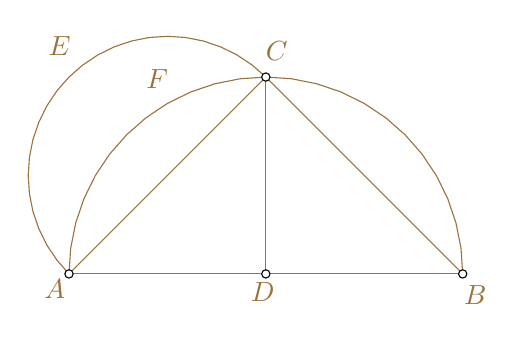
\begin{tikzpicture}
			\draw [shift={(2.5,0.)},lichsutoanhoc]  plot[domain=0.:3.141592653589793,variable=\t]({1.*2.5*cos(\t r)+0.*2.5*sin(\t r)},{0.*2.5*cos(\t r)+1.*2.5*sin(\t r)});
			\draw [lichsutoanhoc] (0.,0.)-- (5.,0.);
			\draw [shift={(1.25,1.25)},lichsutoanhoc]  plot[domain=0.7853981633974483:3.9269908169872414,variable=\t]({1.*1.7677669529663689*cos(\t r)+0.*1.7677669529663689*sin(\t r)},{0.*1.7677669529663689*cos(\t r)+1.*1.7677669529663689*sin(\t r)});
			\draw [lichsutoanhoc] (2.5,2.5)-- (0.,0.);
			\draw [lichsutoanhoc] (2.5,2.5)-- (5.,0.);
			\draw [lichsutoanhoc] (2.5,2.5)-- (2.5,0.);
				\draw [fill=white] (0.,0.) circle (1.5pt);
				\draw[color=lichsutoanhoc] (-0.18,-0.19) node {$A$};
				\draw [fill=white] (5.,0.) circle (1.5pt);
				\draw[color=lichsutoanhoc] (5.16,-0.27) node {$B$};
				\draw[color=lichsutoanhoc] (1.12,2.47) node {$F$};
				\draw [fill=white] (2.5,0.) circle (1.5pt);
				\draw[color=lichsutoanhoc] (2.46,-0.23) node {$D$};
				\draw [fill=white] (2.5,2.5) circle (1.5pt);
				\draw[color=lichsutoanhoc] (2.64,2.83) node {$C$};
				\draw[color=lichsutoanhoc] (-0.12,2.89) node {$E$};
		\end{tikzpicture}
		\caption{\small\textit{\color{lichsutoanhoc}Hình $1a$.}}
		\vspace*{-10pt}
	\end{figure}
	\textit{Chứng minh}. Nối $C$ với $S$. Ký hiệu, thí dụ, ${S_{\bigcirc ACB}}$  là diện tích nửa hình tròn $ACB$ đường kính $AB$. Vì $AB^2 = 2AC^2$  (Hình $1a$)  nên 
	\begin{align*}
		\frac{{{S_{\bigcirc ACB}}}}{{{S_{\bigcirc AEC}}}} = \frac{{\pi {{\left( {\frac{{AB}}{2}} \right)}^2}}}{{\pi {{\left( {\frac{{AC}}{2}} \right)}^2}}} = \frac{{A{B^2}}}{{A{C^2}}} = 2
	\end{align*}
	hay ${S_{\bigcirc ACB}} = 2{S_{\bigcirc AEC}}.$
	\vskip 0.1cm
	Nhưng  ${S_{\bigcirc ACB}} = {S_{\bigcirc ADC}} + {S_{\bigcirc BDC}} = 2{S_{\bigcirc ADC}}$ nên ${S_{\bigcirc AEB}} = {S_{\bigcirc ADC}}$.   Suy ra 
	\begin{align*}
		{S_{AECFA}} + {S_{AFC}} = {S_{AECA}} = {S_{AFCA}} + {S_{\Delta ADC}}.
	\end{align*}
	Vậy diện tích hình trăng khuyết $AECFA$  bằng diện tích tam giác $ADC$,  hay trăng khuyết $AECFA$  đã được ``cầu phương".
	\vskip 0.1cm
	Một phiên bản khác của Định lý $1$ là
	\vskip 0.1cm
	\textbf{\color{lichsutoanhoc}Định lý} $\pmb{1'.}$ Dựng trên các cạnh của tam giác $ABC$ vuông ở $C$   các nửa đường tròn  đường kính $AB, AC, BC$. Khi ấy tổng diện tích hình trăng khuyết $L_1$  và $L_2$ bằng diện tích tam giác  $ABC$ (Hình $1b$).   
	\begin{figure}[H]
%		\vspace*{-5pt}
		\centering
		\captionsetup{labelformat= empty, justification=centering}
		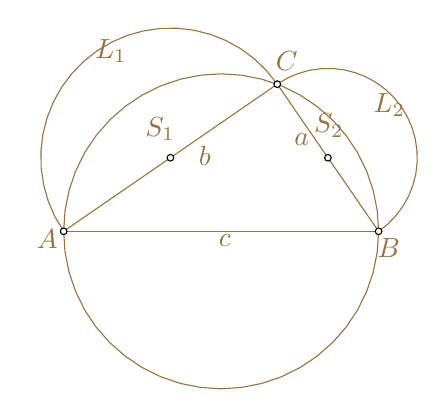
\begin{tikzpicture}[scale=0.8]
			\draw [shift={(2.5,0.)},lichsutoanhoc]  plot[domain=0.:3.141592653589793,variable=\t]({1.*2.5*cos(\t r)+0.*2.5*sin(\t r)},{0.*2.5*cos(\t r)+1.*2.5*sin(\t r)});
			\draw [lichsutoanhoc] (0.,0.)-- (5.,0.);
			\draw [lichsutoanhoc] (3.390811455834727,2.33590559529995)-- (0.,0.);
			\draw [lichsutoanhoc] (3.390811455834727,2.33590559529995)-- (5.,0.);
			\draw [shift={(1.6954057279173635,1.167952797649975)},lichsutoanhoc]  plot[domain=0.6032325047411791:3.744825158330972,variable=\t]({1.*2.058765241544895*cos(\t r)+0.*2.058765241544895*sin(\t r)},{0.*2.058765241544895*cos(\t r)+1.*2.058765241544895*sin(\t r)});
			\draw [shift={(4.195405727917364,1.167952797649975)},lichsutoanhoc]  plot[domain=-0.9675638220537177:2.1740288315360754,variable=\t]({1.*1.418268550101352*cos(\t r)+0.*1.418268550101352*sin(\t r)},{0.*1.418268550101352*cos(\t r)+1.*1.418268550101352*sin(\t r)});
			\draw [shift={(2.5,0.)},lichsutoanhoc]  plot[domain=-3.141592653589793:0.,variable=\t]({1.*2.5*cos(\t r)+0.*2.5*sin(\t r)},{0.*2.5*cos(\t r)+1.*2.5*sin(\t r)});
				\draw [fill=white] (0.,0.) circle (1.5pt);
				\draw[color=lichsutoanhoc] (-0.26,-0.13) node {$A$};
				\draw [fill=white] (5.,0.) circle (1.5pt);
				\draw[color=lichsutoanhoc] (5.16,-0.27) node {$B$};
				\draw[color=lichsutoanhoc] (2.56,-0.15) node {$c$};
				\draw [fill=white] (3.390811455834727,2.33590559529995) circle (1.5pt);
				\draw[color=lichsutoanhoc] (3.54,2.71) node {$C$};
				\draw[color=lichsutoanhoc] (2.24,1.19) node {$b$};
				\draw[color=lichsutoanhoc] (3.78,1.45) node {$a$};
				\draw [fill=white] (1.6954057279173635,1.167952797649975) circle (1.5pt);
				\draw[color=lichsutoanhoc] (1.53,1.62) node {$S_1$};
				\draw [fill=white] (4.195405727917364,1.167952797649975) circle (1.5pt);
				\draw[color=lichsutoanhoc] (4.21,1.68) node {$S_2$};
				\draw[color=lichsutoanhoc] (0.75,2.86) node {$L_1$};
				\draw[color=lichsutoanhoc] (5.17,2.) node {$L_2$};
		\end{tikzpicture}
		\caption{\small\textit{\color{lichsutoanhoc}Hình $1b$.}}
		\vspace*{-10pt}
	\end{figure}
	\textit{Chứng minh}. Ta có   
	\begin{align*}
			{S_{\bigcirc AC}} + {S_{\bigcirc BC}} &= \pi {\left( {\frac{{AC}}{2}} \right)^2} + \pi {\left( {\frac{{BC}}{2}} \right)^2}\\
			&= \frac{\pi }{4}\left( {A{C^2} + B{C^2}} \right) \\
			&= \frac{\pi }{4}A{B^2} = {S_{\bigcirc ABC}}.
	\end{align*}
	Hay (Hình $1b$)
	\begin{align*}
		{S_{{L_1}}} + {S_{{S_1}}} + {S_{{L_2}}} + {S_{{S_2}}} = {S_{\Delta ABC}} + {S_{{S_1}}} + {S_{{S_2}}}.
	\end{align*}
	Suy ra
	\begin{align*}
		{S_{{L_1}}} + {S_{{L_2}}} = {S_{\Delta ABC}}.
	\end{align*}
	\textbf{\color{lichsutoanhoc}Định lý} $\pmb{2}.$ Diện tích nửa lục giác đều $CEFD$ bằng tổng diện tích nửa hình tròn $ALB$  và ba hình trăng khuyết $CGEMC$,  $EHFNE$, $FKDOF$ (Hình $2$).
	\begin{figure}[H]
		\vspace*{-10pt}
		\centering
		\captionsetup{labelformat= empty, justification=centering}
		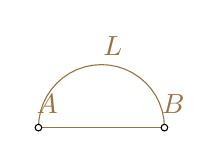
\begin{tikzpicture}[scale=0.8]
			\draw [lichsutoanhoc] (-5.,0.)-- (-3.,0.);
			\draw [shift={(-4.,0.)},lichsutoanhoc]  plot[domain=0.:3.141592653589793,variable=\t]({1.*1.*cos(\t r)+0.*1.*sin(\t r)},{0.*1.*cos(\t r)+1.*1.*sin(\t r)});
			
			\draw [fill=white] (-5.,0.) circle (1.5pt);
			\draw[color=lichsutoanhoc] (-4.86,0.37) node {$A$};
			\draw [fill=white] (-3.,0.) circle (1.5pt);
			\draw[color=lichsutoanhoc] (-2.86,0.37) node {$B$};
			
			\draw[color=lichsutoanhoc] (-3.82,1.29) node {$L$};
		\end{tikzpicture}
		\caption{\small\textit{\color{lichsutoanhoc}Hình $2a$.}}
		\vspace*{-10pt}
	\end{figure}
	\begin{figure}[H]
		\vspace*{-10pt}
		\centering
		\captionsetup{labelformat= empty, justification=centering}
		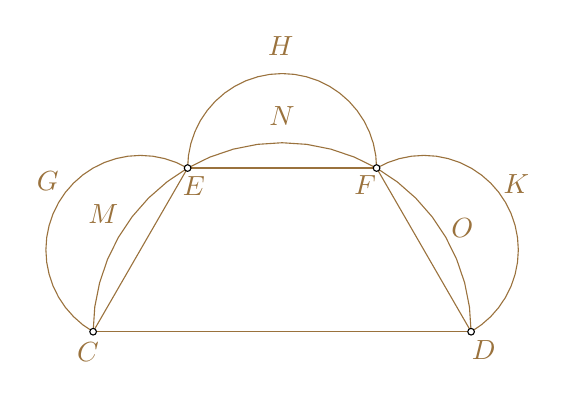
\begin{tikzpicture}[scale=0.8]
			\draw [lichsutoanhoc] (-1.,0.)-- (5.,0.);
			\draw [shift={(2.,0.)},lichsutoanhoc]  plot[domain=0.:3.141592653589793,variable=\t]({1.*3.*cos(\t r)+0.*3.*sin(\t r)},{0.*3.*cos(\t r)+1.*3.*sin(\t r)});
			\draw [shift={(-0.25,1.299038105676658)},lichsutoanhoc]  plot[domain=1.0471975511965979:4.188790204786391,variable=\t]({1.*1.5*cos(\t r)+0.*1.5*sin(\t r)},{0.*1.5*cos(\t r)+1.*1.5*sin(\t r)});
			\draw [shift={(2.,2.598076211353316)},lichsutoanhoc]  plot[domain=0.:3.141592653589793,variable=\t]({1.*1.5*cos(\t r)+0.*1.5*sin(\t r)},{0.*1.5*cos(\t r)+1.*1.5*sin(\t r)});
			\draw [shift={(4.25,1.299038105676658)},lichsutoanhoc]  plot[domain=-1.0471975511965983:2.0943951023931953,variable=\t]({1.*1.5*cos(\t r)+0.*1.5*sin(\t r)},{0.*1.5*cos(\t r)+1.*1.5*sin(\t r)});
			\draw [lichsutoanhoc] (-1.,0.)-- (0.5,2.598076211353316);
			\draw [lichsutoanhoc] (0.5,2.598076211353316)-- (3.5,2.598076211353316);
			\draw [lichsutoanhoc] (3.5,2.598076211353316)-- (5.,0.);
		
				\draw [fill=white] (-1.,0.) circle (1.5pt);
				\draw[color=lichsutoanhoc] (-1.08,-0.33) node {$C$};
				\draw [fill=white] (5.,0.) circle (1.5pt);
				\draw[color=lichsutoanhoc] (5.2,-0.29) node {$D$};
				\draw [fill=white] (0.5,2.598076211353316) circle (1.5pt);
				\draw[color=lichsutoanhoc] (0.6,2.31) node {$E$};
				\draw [fill=white] (3.5,2.598076211353316) circle (1.5pt);
				\draw[color=lichsutoanhoc] (3.32,2.33) node {$F$};
				\draw[color=lichsutoanhoc] (-1.72,2.39) node {$G$};
				\draw[color=lichsutoanhoc] (1.98,4.53) node {$H$};
				\draw[color=lichsutoanhoc] (5.72,2.35) node {$K$};
				\draw[color=lichsutoanhoc] (-0.84,1.87) node {$M$};
				\draw[color=lichsutoanhoc] (2.,3.43) node {$N$};
				\draw[color=lichsutoanhoc] (4.86,1.65) node {$O$};
		\end{tikzpicture}
		\caption{\small\textit{\color{lichsutoanhoc}Hình $2b$.}}
		\vspace*{-5pt}
	\end{figure}
	\textit{Chứng minh}. Dựng nửa hình tròn đường kính $AB = \dfrac{1}{2}CD$ (Hình $2a$). Dựng các nửa hình tròn đường kính $CE, EF, FD$ là ba cạnh liên tiếp của lục giác đều nội tiếp đường tròn đường kính  $CD$ (Hình $2b$). Vì 
	\begin{align*}
		C{D^2} = 4A{B^2} = A{B^2} + C{E^2} + E{F^2} + F{D^2}
	\end{align*}
	và tỷ lệ diện tích các hình tròn bằng tỷ lệ diện tích các hình vuông dựng trên đường kính của chúng nên 
	\begin{align*}
		&{S_{\bigcirc CEFD}} \\
		= &{S_{\bigcirc ALB}} + {S_{\bigcirc CGE}} + {S_{\bigcirc EHF}} + {S_{\bigcirc FKD}}.
	\end{align*}
	Trừ hai vế cho tổng diện tích ba hình viên phân $CMEC, ENFE, FODF$  ta được  
	\begin{align*}
		&{S_{CEFD}} \\
		= &{S_{\bigcirc ALB}} + {S_{CGEMC}} + {S_{EHFNE}} + {S_{FKDOF}}.
	\end{align*}
	Eudemus tin rằng Hippocrates đã chứng minh hai định lý trên, nhưng một chứng minh nghiêm túc vào thời điểm đó (khoảng năm $430$ trước Công nguyên) dường như khó có thể xảy ra. Chứng minh trong Quyển $12$ Chương $2$ \textit{Cơ sở} của Euclid dường như là của Eudoxus, một nhà toán học sống nửa thời gian giữa Hippocrates và Euclid. Tuy nhiên, hai cuốn sách đầu của Euclid dường như bắt nguồn từ Pythagoras, vì vậy sẽ có vẻ hợp lý khi giả định rằng công thức, ít nhất, phần lớn cuốn sách III và IV của \textit{Cơ sở}  là từ tác phẩm của Hippocrates. Hơn nữa, nếu Hippocrates đã đưa ra một chứng minh định lý về diện tích của các hình giới hạn bởi các hình tròn, thì Hippocrates chính là người phát minh ra phương pháp chứng minh gián tiếp trong toán học. 
	\vskip 0.1cm
	Từ các định lý về diện tích hình trăng khuyết, Hippocrates được coi là người đầu tiên trong lịch sử toán học tìm ra cách tính diện tích các hình cong (khác hình tròn). 
	\vskip 0.1cm
	Có cơ sở tương đối vững chắc về mặt lịch sử  khi nói rằng cầu phương hình tròn đã được phát triển bởi Hippocrates. Các học giả ngoài Simplicius cũng đề cập đến tác phẩm của Hippocrates. Simplicius sống ở thế kỷ VI, nhưng ông không chỉ trích dẫn Eudemus (khoảng năm $320$ TCN) mà còn dựa vào Alexander xứ Aphrodisias (khoảng năm $200$ CN), một trong những nhà bình luận chính về Aristotle. 
	Các kết quả trên dường như đã khuyến khích Hippocrates, cũng như những người cùng thời và những người kế nhiệm ông hi vọng rằng cuối cùng hình tròn sẽ được cầu phương.
	\vskip 0.1cm
	Các kết quả của Hippocrates về cầu phương hình trăng khuyết có thể coi là những nỗ lực đáng kể của toán học vào thời điểm đó. Nó cho thấy rằng các nhà toán học Athens rất thành thạo trong việc xử lý các phép biến đổi diện tích và tỷ lệ.
	\vskip 0.1cm 
	Có ba quan điểm về những gì Hippocrates đã suy luận từ cầu phương hình trăng khuyết. Một số đã buộc tội Ông vì tin rằng Ông có thể cầu phương tất cả các hình trăng, trong đó có hình tròn; Những người khác nghĩ rằng Ông biết những hạn chế công việc của mình, biết rằng nó được chứng minh chỉ với một số loại hình trăng. Một học giả lại viết rằng Hippocrates biết Ông đã không cầu phương hình tròn nhưng cố đánh lừa đồng hương là mình đã thành công. 
	\vskip 0.1cm
	Hippocrates còn là người đầu tiên sử dụng ký hiệu chữ cái trong các hình hình học. Thật thú vị khi lưu ý rằng trong khi Hippocrates có đóng góp trong hai bài toán nổi tiếng, Ông dường như đã không có tiến bộ trong bài toán chia ba một góc, một vấn đề được nghiên cứu phần nào sau đó bởi Hippias của Elis.
	\vskip 0.1cm
	\textbf{\color{lichsutoanhoc}Hippias xứ Elis}
	\vskip 0.1cm
	Vào cuối thế kỷ thứ năm TCN, một nhóm giáo viên chuyên nghiệp hoàn toàn không giống như người Pythagoras nổi lên mạnh mẽ ở Athens. Trong số này có Hippias, một người gốc Elis, đã sống tại Athens vào nửa sau của thế kỷ thứ năm TCN.  Ông là một trong những nhà toán học đầu tiên mà chúng ta có thông tin trực tiếp, vì chúng ta đọc được nhiều điều về Ông từ \textit{Đối thoại} của Plato. Ông được cho là đã viết nhiều, từ toán học để diễn xướng, nhưng không có tác phẩm nào của Ông còn tồn tại.  
	\vskip 0.1cm
	Hippias (khoảng $500-401$ TCN)  sống cùng thời với Socrates (khoảng $477-399$ TCN). Socrates được cho là đã mô tả Hippias đẹp trai, học giỏi nhưng khoe khoang và nông nổi. Trong \textit{Đối thoại} của Plato và \textit{Những kỷ vật} của Xenophon có những nhận xét không mấy hay ho về Hippias như một người tự coi mình là một chuyên gia trong mọi thứ từ lịch sử và văn học đến thủ công mỹ nghệ và khoa học. 
	\vskip 0.1cm
	Proclus và các nhà toán học khác đã gán tên trisectrix hoặc quadratrix cho Hippias, các đường cong khác đường tròn và đường thẳng. Điều này được mô tả như sau: Trong hình vuông $ABCD$ (Hình $3$), cho cạnh $AB$ di chuyển đều từ vị trí hiện tại của nó cho đến khi nó trùng với $DC$ và để chuyển động này diễn ra chính xác cùng thời gian $DA$ quay theo chiều kim đồng hồ từ vị trí hiện tại của nó cho đến khi nó trùng với $DC$.
	\begin{figure}[H]
		\vspace*{-5pt}
		\centering
		\captionsetup{labelformat= empty, justification=centering}
		\includegraphics[width = 0.85\linewidth]{1}
		\caption{\small\textit{\color{lichsutoanhoc}Hình $3$.}}
		\vspace*{-10pt}
	\end{figure}
	Nếu vị trí của hai đường chuyển động tại bất kỳ thời gian tương ứng được cho bởi $AuBu$ và $DAv$, và nếu $P$ là điểm của giao điểm của $AuBu$ và $DAv$, quỹ tích của $P$ trong quá trình chuyển động sẽ là trisectrix của Hippias -- đường cong $APQ$ trong Hình $3$. Với đường cong này, việc cắt bỏ một góc được thực hiện một cách dễ dàng. Ví dụ: nếu $PDC$ là góc được cắt bỏ, người ta chỉ cần cắt các đoạn $BuC$ và $AuD$ tại các điểm $R$, $S$, $T$ và $U$. Nếu đường $TR$ và $US$ cắt trisectrix ở $V$ và $W$, tương ứng, các dòng $VD$ và $WD$, theo thuộc tính của trisectrix, chia góc $PDC$ thành ba phần bằng nhau. Đường cong Hippias thường được gọi là quadratrix, vì nó có thể được sử dụng để cầu phương hình tròn. Người ta đã phỏng đoán rằng Hippias biết về phương pháp cầu phương này nhưng cầu phương qua đường cong Hippias do Dinostratus đưa ra sau này.
	\vskip 0.1cm
	Về tính cách, Plato đối lập Hippias với Socrates, người ta có thể tạo ra nhiều sự tương phản giống nhau bằng cách so sánh Hippias với một người cùng thời khác--nhà toán học thuộc trường phái Pythagoras là Archytas xứ Tarentum.
	\vskip 0.1cm
	\textbf{\color{lichsutoanhoc}Philolaus và Archytas xứ Tarentum}
	\vskip 0.1cm  
	Pythagoras được cho là đã lui về Metapontum vào cuối đời và đã chết ở đó khoảng năm $500$ TCN.  Ông không để lại các tác phẩm viết, nhưng ý tưởng của Ông đã được thực hiện bởi một số lượng lớn đệ tử. Trung tâm ở Croton đã bị bỏ hoang khi một nhóm đối thủ chính trị từ Sybaris đã bất ngờ sát hại nhiều thủ lĩnh, nhưng những người thoát khỏi vụ thảm sát đã mang theo các học thuyết của trường phái Pythagoras đến các khu vực khác của thế giới Hy Lạp. Trong số những người học được từ những người tị nạn Pythagoras có Philolaus xứ Tarentum. Ông được cho là đã viết bài tường thuật đầu tiên về thuyết Pythagoras.  Rõ ràng, đây là cuốn sách mà từ đó Plato rút ra kiến thức của Ông về Pythagoras.  
	\vskip 0.1cm
	Sự cuồng tín số rất đặc trưng của Pythagoras hiển nhiên đã được chia sẻ bởi Philolaus. Ông giải thích phần lớn những truyền thuyết huyền bí cũng như kiến thức về vũ trụ học của Pythagoras. Các Sơ đồ vũ trụ của Philolaus được cho là đã được sửa đổi bởi hai người thuộc trường phái Pythagoras, Ecphantus và Hicetas, những người đã giải thích ngày và đêm bằng cách đặt trái đất quay.  
	\vskip 0.1cm
	Sự cực đoan của việc tôn thờ số của Philolaus dường như cũng đã trải qua một số sửa đổi, đặc biệt hơn là dưới bàn tay của Archytas, một học trò của Philolaus xứ Tarentum. 
	\vskip 0.1cm
	Archytas tin tưởng chắc chắn vào hiệu quả của số. Trong nhiều năm liên tiếp, ông được bầu làm tướng, và Ông chưa bao giờ bị đánh bại. Ông tốt bụng và là một người yêu trẻ em, vì Ông là được cho là đã phát minh ra ``rchytas's rattle", một đồ chơi bằng gỗ, được chế tạo để làm thú vui cho trẻ. Archytas tiếp tục truyền thống Pythagoras trong việc đặt số học lên trên hình học, nhưng sự nhiệt tình của Ông đối với con số nhẹ hơn ở Philolaus.  Ông đã viết ứng dụng của số học, hình học đối với âm nhạc, và có thể là Philolaus hoặc Archytas đã đưa ra khái niệm ``trung bình điều hòa". 
	\vskip 0.1cm
	Archytas đã chú ý nhiều đến âm nhạc nhiều hơn so với những người tiền nhiệm của mình và Ông cảm thấy rằng môn học này phải đóng một vai trò lớn hơn văn học trong việc giáo dục trẻ em. Archytas dường như đã chú ý đáng kể đến vai trò của toán học trong chương trình giảng dạy, và Ông được coi là đã chỉ định bốn nhánh trong tứ giác toán học -- số học (hoặc số còn lại), hình học (hoặc độ lớn khi dừng lại), âm nhạc (hoặc các con số đang chuyển động) và thiên văn học (hoặc độ lớn trong chuyển động). Các môn học này, cùng với bộ ba bao gồm ngữ pháp, tu từ và biện chứng (mà Aristotle bắt nguồn từ Zeno), sau này tạo thành bảy nghệ thuật tự do; vì thế Archytas được coi là có đóng góp nổi bật đưa vai trò của toán học lên một vị trí quan trọng trong giáo dục. 
	\vskip 0.1cm
	Tuy nhiên, đóng góp quan trọng nhất của Archytas cho toán học có thể là sự can thiệp của ông với bạo chúa Dionysius để cứu sống người bạn Plato của mình. Plato cho đến cuối cuộc đời vẫn cam kết sâu sắc với sự tôn kính Pythagoras về số và hình học, và vị thế tối cao của Athens trong thế giới toán học của thế kỷ thứ tư TCN là kết quả chủ yếu từ sự nhiệt tình của Plato, ``nhà tạo ra các nhà toán học." 
	\vskip 0.1cm
	\textbf{\color{lichsutoanhoc}Menaechmus}
	\vskip 0.1cm
	Eudoxus được ghi nhớ trong lịch sử toán học không chỉ vì công việc của riêng mình mà còn thông qua học sinh của mình. 
	\vskip 0.1cm
	Ở Hy Lạp, có một sợi dây tiếp nối truyền thống từ thầy sang trò.  Thí dụ, Plato học được từ Archytas, Theodorus và Theaetetus; ảnh hưởng của Plato lần lượt được truyền qua Eudoxus cho anh em Menaechmus và Dinostratus, cả hai đều đạt được thành tựu xuất sắc trong toán học. 
	\vskip 0.1cm
	Menaechmus nổi tiếng là người đã khám phá ra các đường cong mà sau này được gọi là hình elip, parabol và hyperbol, các thiết diện được cắt ra bởi hình nón (các đường cong conic).
	\vskip 0.1cm
	Menaechmus đã thành công dựa trên các đường cong conic với các tính chất thích hợp để giải bài toán gấp đôi khối lập phương. 
	\vskip 0.1cm
	Proclus đã viết rằng Menaechmus là một trong những người đã ``làm cho toàn bộ hình học trở lên hoàn hảo hơn" (made the whole of geometry more perfect). Chúng ta biết rằng Menaechmus đã dạy Alexander Đại đế, và huyền thoại nổi tiếng thuộc về Menaechmus, khi học trò của Ông yêu cầu một lối tắt đến hình học: ``Hỡi Vua, để đi qua đất nước, có những con đường hoàng gia và những con đường dành cho công dân chung; nhưng trong hình học, chỉ có một con đường cho tất cả mọi người". ``O King, for traveling over the
	country there are royal roads and roads for common citizens; but in geometry there is one road for all."
	\vskip 0.1cm 
	Chứng cứ Menaechmus phát hiện ra các thiết diện conic là do một lá thư từ Eratosthenes đến Vua Ptolemy Euergetes, được Eutocius trích dẫn khoảng $700$ năm sau đó, trong đó bài toán gấp đôi khối lập phương được đề cập. 
	\vskip 0.1cm
	\textbf{\color{lichsutoanhoc}Dinostratus và cầu phương hình tròn}
	\vskip 0.1cm
	Dinostratus, anh trai của Menaechmus, cũng là một nhà toán học; một người đã ``giải quyết" bài toán gấp đôi khối lập phương, người còn lại ``giải quyết" bài toán cầu phương hình tròn. 
	\vskip 0.1cm
	\textbf{\color{lichsutoanhoc}Thay lời kết}
	\vskip 0.1cm
	Tất nhiên, người Hy Lạp cũng hiểu rằng việc sử dụng đường cong trong các bài toán chia ba góc và các bài toán cầu phương đã vi phạm quy tắc của trò chơi—chỉ cho phép sử dụng compass và thước thẳng. ``Lời giải" của Hippias, Menaechmus và Dinostratus, như các tác giả của chúng cũng nhận ra, là ngụy tạo; vì thế, việc tìm kiếm các giải pháp khác, chính tắc hoặc bất hợp pháp, tiếp tục, với kết quả là một số đường cong mới đã được phát hiện bởi các nhà hình học Hy Lạp.
	\vskip 0.1cm
	\textbf{\color{lichsutoanhoc}Tài liệu tham khảo chính}
	\vskip 0.1cm
	[$1$] David M. Burton, \textit{The History of Mathematics, An Introduction, Seventh Edition}, McGraw--Hill, $2011$. Chapter $3$: The Beginnings of Greek Mathematics, $3.2$ Pythagorean Mathematics, pp. $116-139$.
	\vskip 0.1cm
	[$2$] Thomas Heath, \textit{A History of Greek Mathematics, Oxford at the Clarendon Press}, $1921$, Volume $1$: From Thales to Euclid, pp. $170-353$.
	\vskip 0.1cm   
	[$3$] Victor J. Katz, \textit{A History of Mathematics, An Introduction}, Third Edition, Addison--Wesley, $2009$. Chapter $2$: \textit{The Beginnings of Mathematics in Greek}, pp. $40-49$.
	\vskip 0.1cm
	[$4$] Uta C. Merzbach and Carl B. Boyer, \textit{A
	History of Mathematics}, Third Edition, John Wiley \& Sons, $2011$, trang $57-89$.
	\vskip 0.1cm
	[$5$] Ngô Việt Trung, \textit{Lý thuyết Galois về các vấn đề giải phương trình bằng căn thức, dựng hình bằng thước kẻ và compa}, Nhà xuất bản Đại học Quốc gia Hà Nội, $2006$.
	\vskip 0.1cm
	\textbf{\color{lichsutoanhoc}Tài liệu tham khảo}
	\vskip 0.1cm 
	[$6$] George Johston Allman, \textit{Greek Geometry: From Thales to Euclid}, Dublin Universty Press, $1877$, $432$ trang.  
	\vskip 0.1cm
	[$7$] Euclid, \textit{Cơ sở của Hình học}, Nhà xuất bản Trí thức, $2016$, $350$ trang.
	\vskip 0.1cm
	[$8$] R. Lloyd, \textit{Early Greek Science: Thales to Aristotle}, $1970$, Chatto \& Windus, London, $156$ trang. 
	\vskip 0.1cm
	[$8$] Nicomachus of Gerasa, \textit{Introduction to Arithmetic}, Translated into English by Martin Luther D’ooge, The Macmillan Company, New York, $1926$.
	\vskip 0.1cm
	[$9$] Proclus, \textit{Commentaries on Euclid’s books}, Vol. $1$, $330$ trang.
	\vskip 0.1cm
	[$10$] Arpad Szabo, \textit{The beginnings of Greek Mathematics}, Springer, $1978$, $363$ trang.
	\vskip 0.1cm
	[$11$] M. L. West, \textit{Early Greek Philosophy and the Orient}, Oxford at the Clarendon Press, $1971$, $255$ trang.
\end{multicols}
	 \newpage

%	 \setcounter{figure}{0}
%	 \thispagestyle{diendandayvahoctoannone}
\pagestyle{diendandayvahoctoan}
\everymath{\color{diendantoanhoc}}
\graphicspath{{../diendantoanhoc/pic/}}
\blfootnote{$^{1}$\color[named]{diendantoanhoc}Thái Nguyên.}
\begingroup
\AddToShipoutPicture*{\put(0,616){\includegraphics[width=19.3cm]{../bannerdiendan}}}
\AddToShipoutPicture*{\put(44,525){\includegraphics[scale=1]{../tieude2.pdf}}}
\centering
\endgroup
\vspace*{192pt}

Trong bài viết này, tác giả xin giới thiệu với bạn đọc phương pháp sử dụng tiếp tuyến để giải một số bài toán về phương trình, bất phương trình thông qua tính lồi, lõm của hàm số.

\begin{multicols}{2}
	\textbf{\color{diendantoanhoc}$\pmb{1.}$ Khái niệm về tính lồi, lõm và điểm uốn của đồ thị}
	\vskip 0.1cm
	Xét đồ thị $ACB$ của hàm số $y = f(x)$ biểu diễn trong hình dưới đây. Ta giả thiết rằng tại mọi điểm của nó, đồ thị đã cho đều có tiếp tuyến. Tại mọi điểm của cung $AC$ tiếp tuyến luôn luôn ở \emph{phía trên} của $AC$, ta nói $AC$ là một \textbf{\color{diendantoanhoc}\itshape cung lồi}. Nếu $a$ là hoành độ của $A$ và $c$ là hoành độ của $C$, thì khoảng $(a; c)$ được gọi là một khoảng lồi của đồ thị. Tại mỗi điểm của cung $CB$ tiếp tuyến luôn luôn ở \emph{\itshape phía dưới} của $CB$. Ta nói $CB$ là một \textbf{\color{diendantoanhoc}\itshape cung lõm}. Nếu $c$ là hoành độ của $C$, $b$ là hoành độ của $B$ thì khoảng $(c; b)$ được gọi là một khoảng lõm của đồ thị.
	\begin{center}
		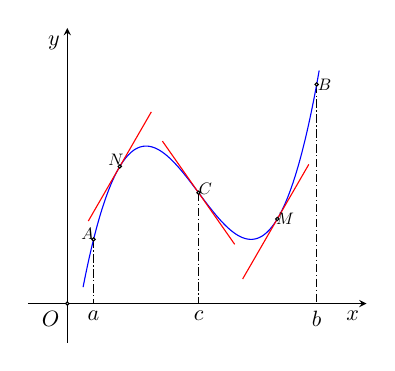
\begin{tikzpicture}
			\def\hsf(#1){((#1)^3-5*(#1)^2+7*(#1)-1}%ham so f
			\draw[-stealth,very thin](-.5,0)--(3.8,0)node[below left,scale=.8]{$x$};%truc Ox
			\draw[-stealth,very thin](0,-.5)--(0,3.5) node[below left,scale=.8]{$y$};%truc Oy
			\draw[fill=white](0,0)circle(.6pt)node[below left,scale=.8]{$O$};%goc toa do O
			\path (1/3,{\hsf(1/3)})coordinate(A) (19/6,{\hsf(19/6)})coordinate(B) (5/3,{\hsf(5/3)})coordinate(C)
			(8/3,{\hsf(8/3)})coordinate(M) (2/3,{\hsf(2/3)})coordinate(N);
			\draw[color=black,densely dash dot, thin] (A)--(1/3,0)node[below ,scale=.8] {$a$} (B)--(19/6,0)node[below ,scale=.8] {$b$} (C)--(5/3,0)node[below ,scale=.8] {$c$};
			\draw[blue,smooth,samples=100] plot[domain=.2:3.2](\x,{\hsf(\x)});
			\draw[red] (C)--+(125:.8)(C)--+(-55:.8) 
			(N)--+(60:.8)(N)--+(-120:.8) 
			(M)--+(60:.8)(M)--+(-120:.88);
			\foreach \p/\g in{A/140,B/0,C/30,M/0,N/120} \draw[fill=white](\p)circle(.6pt)+(\g:.1)node[scale=.6]{$\p$};
		\end{tikzpicture}
	\end{center}
	Điểm phân cách giữa cung lồi và cung lõm được gọi là \textbf{\color{diendantoanhoc}\itshape điểm uốn}. Điểm $C$ của đồ thị trong hình là điểm uốn.
	\vskip 0.1cm
	Nói cách khác thì: 
	Nếu hàm số $y=f(x)$ có đạo hàm trên khoảng ($I$ ). Ta nói rằng
	\vskip 0.1cm
	$a)$ Đồ thị ($C$) của hàm số $y = f(x)$ lồi trên khoảng ($I$) nếu tiếp tuyến của ($C$) tại mỗi điểm của nó đều nằm phía trên đồ thị.
	\vskip 0.1cm
	$b)$ Đồ thị ($C$) của hàm số $ y = f(x)$ lõm trên khoảng ($I$) nếu tiếp tuyến của nó tại mỗi điểm của nó đều nằm phía dưới đồ thị.
	\vskip 0.1cm
	Nhận xét: Đồ thị hàm lồi có hình dạng giống như một cái mũ $\cap $ còn của hàm lõm thì có hình dạng giống như một cái cốc  $\cup $.
	\vskip 0.1cm
	\textbf{\color{diendantoanhoc}$\pmb{2.}$ Dấu hiệu lồi, lõm và điểm uốn của đồ thị}
	\vskip 0.1cm
	Ta thừa nhận dấu hiệu lồi, lõm sau đây:
	\vskip 0.1cm
	Định lý: Cho hàm số $y = f(x)$ có đạo hàm đến cấp hai trên khoảng $I$.
	\vskip 0.1cm
	$1)$ Nếu $f "(x)< 0$ với mọi $x\in I$ thì đồ thị của hàm số \textbf{\color{diendantoanhoc}\itshape lồi} trên khoảng đó. 
	\vskip 0.1cm
	$2)$ Nếu $f "(x)> 0$ với mọi $x\in I$ thì đồ thị của hàm số  \textbf{\color{diendantoanhoc}\itshape lõm} trên khoảng đó.
	\vskip 0.1cm
	Định lý: Giả sử hàm số $y = f(x)$ có đạo hàm cấp hai trên một khoảng $I$ chứa điểm $ x _0$. Nếu $f"(x_0) = 0$ và $f"(x) $ đổi dấu khi $x$ qua điểm $x_0$ thì $U(x_0;f(x_0))$ là một điểm uốn của đồ thị hàm số $y = f(x)$.
	\vskip 0.1cm
	Tại điểm uốn tiếp tuyến đi xuyên qua đồ thị.
	\vskip 0.1cm
	\textbf{\color{diendantoanhoc}$\pmb{3.}$ Điều kiện để hai đường cong tiếp xúc nhau}
	\vskip 0.1cm
	Điều kiện để hai đường cong $y= f(x)$ và $y=g(x) $ tiếp xúc nhau là hệ phương trình sau có nghiệm và nghiệm của hệ là hoành độ giao điểm của hai đường cong đó \begin{align*}
		\begin{cases}f(x)=g(x)\\ f'(x)=g'(x)\end{cases}\tag{$*$}
	\end{align*}
	Vậy $f$ và $g$ tiếp xúc nhau khi và chỉ khi $x_0$ là nghiệm của hệ ($*$).
	\vskip 0.1cm
	Nếu hai đường cong $y=f(x)$ và $y=g(x)$ có tính lồi lõm trái ngược nhau, ngoài ra có chung nhau tiếp tuyến thì khi đó phương trình $f(x)=g(x)$ có nghiệm duy nhất.
	\begin{center}
		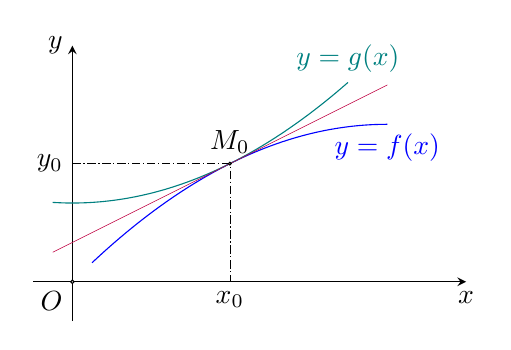
\begin{tikzpicture}
			\def\hsf(#1){-.125*(#1)^2+(#1)}%ham so f
			\def\hsg(#1){.125*(#1)^2+1}%ham so g
			\draw[-stealth] (-.5,0)--(5,0)node[below]{$x$};
			\draw[-stealth] (0,-.5)--(0,3)node[left]{$y$};
			\draw[fill=white](0,0)circle(.6pt)node[below left]{$O$};
			\draw[densely dash dot,very thin] (0,3/2)node[left]{$y_0$}-|(2,0) node[below]{$x_0$};
			\draw[smooth,blue]plot[domain=.25:4](\x,{\hsf(\x)}) node[below]{$y=f(x)$};
			\draw[smooth,teal]plot[domain=-.25:3.5](\x,{\hsg(\x)}) node[above]{$y=g(x)$};
			\draw[smooth,very thin,purple]plot[domain=-.25:4](\x,{.5*\x+1/2});
			\draw[fill=white](2,3/2)circle(.5pt)node[above]{$M_0$};
		\end{tikzpicture}
	\end{center}
	Cần phải chú ý rằng nhiều tài liệu trong và ngoài nước hiện nay định nghĩa về tính lồi (convex), lõm (concave) của đồ thị hàm số khác như đã nêu ở trên. Cụ thể là hàm lồi trong bài viết này được gọi là hàm lõm trong một số tài liệu, còn hàm lõm trong bài viết này thì lại được họ gọi là hàm lồi. 
	\vskip 0.1cm
	\textit{\textbf{\color{diendantoanhoc}Ta sẽ vận dụng những tính chất và nhận xét trên để ứng dụng trong việc giải một số bài toán về phương trình, bất phương trình, đây cũng chính là cở sở của phương pháp tiếp tuyến trên}}.
	\vskip 0.1cm
	Trong bài viết này chúng ta viết tắt VT cho vế trái, VP cho vế phải.
	Việc kiểm tra dấu hiệu lồi, lõm của hàm số bằng cách tính đạo hàm cấp hai trong một số ví dụ sẽ được dành cho bạn đọc.
	\vskip 0.1cm
	\textbf{\color{diendantoanhoc}$\pmb{4.}$ Các ví dụ}
	\vskip 0.1cm
	\textbf{\color{diendantoanhoc}Ví dụ $\pmb{1.}$} Giải phương trình
	\begin{align*}
		x^2-2x+5=\sqrt{x+3}+\sqrt{5-x}.
	\end{align*}
	\textit{Lời giải.} Điều kiện $-3\leq x\leq 5$. Vế trái là hàm lõm còn vế phải là hàm lồi (bạn đọc tự kiểm tra), chúng có chung tiếp tuyến tại $x=1$ là $y=4$. Vậy $x=1$ là nghiệm duy nhất.
	\vskip 0.1cm
	Nhận xét: Bài tập kiểu như trên rất quen thuộc với nhiều bạn đọc, phương pháp thường dùng là đánh giá bất đẳng thức. Ở đây, chúng ta sử dụng tiếp cận mới thông qua tiếp tuyến.
	\vskip 0.1cm
	Ta sẽ đến với những ví dụ khác, đòi hỏi đến cả kỹ năng nhẩm nghiệm.
	\vskip 0.1cm
	\textbf{\color{diendantoanhoc}Ví dụ $\pmb{2.}$} Giải phương trình
	\begin{align*}
		\sqrt[6]{6x-5}=\dfrac{x^{7}}{8x^{2}-10x+3}.
	\end{align*}
	\textit{Lời giải.} Điều kiện $x\ge \frac{5}{6}$. Với $x\ge \frac{5}{6}$ thì $VT$ là hàm lồi, liên tục, vì vậy đồ thị hàm số nằm dưới tất cả các tiếp tuyến của nó tại điểm $x=1$ là $y=x+1$.
	Với $x\ge\frac{5}{6}$ thì $VP$ là hàm lõm, liên tục, vì vậy đồ thị hàm số nằm trên tất cả các tiếp tuyến của nó tại điểm $x=1$ là $y=x+1$.
	\vskip 0.1cm
	Vậy $x=1$ là nghiệm duy nhất của phương trình. 
	\vskip 0.1cm
	\textbf{\color{diendantoanhoc}Ví dụ $\pmb{3.}$} Cho hai hàm số $f(x)$ và $g(x)$ được xác định như sau: $f(x)=\sqrt{13x^{2} - 6x + 10 } + \sqrt{5x^{2} -13x + \frac{17}{2}} + \sqrt{17x^{2} - 48x + 36} $ và $g(x)= \dfrac{1}{2}(36x - 8x^{2} - 21)$.
	\vskip 0.1cm
	Giải phương trình $f(x)=g(x)$.
	\vskip 0.1cm
	\textit{Lời giải.} Điều kiện $x\in \mathbb R$. Đặt $h(x)=f(x)-g(x)$\\ Không khó để chỉ ra $h(x)$ là hàm lõm, liên tục. Nhận thấy $h(\dfrac{3}{2})=0$ và $h'(\dfrac 32)=0$ , do đó đồ thị hàm số tiếp xúc với trục hoành tại điểm $x=\dfrac{3}{2}$.
	\vskip 0.1cm
	Vậy $x=\dfrac{3}{2}$ là nghiệm duy nhất của phương trình của bài toán.
	\vskip 0.1cm
	\textbf{\color{diendantoanhoc}Ví dụ $\pmb{4.}$} Giải phương trình
	\begin{align*}
		x\sqrt{x^2\!+\!6}\!+\!(x\!+\!1)\sqrt{x^2\!+\!2x\!+\!7}\!=\!\dfrac{13}{5}(2x\!+\!1)
	\end{align*}
	\textit{Lời giải.}  Điều kiện $x\in\mathbb R$. Đặt $g(x)=x\sqrt{x^2+6}$ và $f(x)=g(x+1)+g(x)$.
	\vskip 0.1cm
	Ta dễ kiểm tra thấy rằng:
	\vskip 0.1cm
	$a)$ $g(x)$ là hàm lẻ và $g''(x)$ cũng là hàm lẻ; hơn nữa ta cũng có $f(-\dfrac 12)=f''(-\dfrac 12)=0$.
	\vskip 0.1cm
	$b)$ $g(x)$ và $g''(x)$ là hàm đồng biến, suy ra $f(x)$ và $f''(x)$ cũng là hàm đồng biến.
	\vskip 0.1cm
	$c)$ Tiếp tuyến $f(x)$ tại $x=-\dfrac 12$ là $y=\dfrac{13}5(2x+1)$.
	\vskip 0.1cm
	Vậy đồ thị hàm số $f(x)$ nằm dưới tiếp tuyến của nó khi $x<-\dfrac 12$ và đồ thị hàm số $f(x)$ nằm trên tiếp tuyến của nó khi $x>-\dfrac 12$.
	\vskip 0.1cm
	Vậy $x=-\dfrac{1}{2}$ là nghiệm duy nhất của phương trình.
	\vskip 0.1cm
	Chú ý: Ở ví dụ này nghiệm của phương trình chính là điểm uốn của đồ thị.
	\vskip 0.1cm
	\textbf{\color{diendantoanhoc}Ví dụ $\pmb{5.}$} Giải phương trình
	\begin{align*}
		&3\left(x^{3}+\frac{x}{\sqrt{\left(1+x^{2} \right)^{3}}} \right)+2\\
		=\,\,&\sqrt{\left(1+x \right)^{3}}+\sqrt{\left(1-x \right)^{3}}.
	\end{align*}
	\textit{Lời giải.}  Điều kiện xác định $x\in[-1;1]$. Nhận xét rằng $x=0$ là một nghiệm của phương trình. Đặt $f(x)=x+(1+x)^{-\frac 32}$ và $g(x)=\dfrac{(1+x)^{\frac 32}+(1-x)^{\frac 32}-2}x$.
	\vskip 0.1cm
	Giả sử $x\ne 0$. Phương trình đã cho có thể được viết lại thành $3f(x^2)=g(x)$.
	\vskip 0.1cm
	Chú ý rằng:
	\vskip 0.1cm
	Một mặt, $g(x)$ là hàm lẻ, nhận giá trị âm trên $[-1;0)$ và dương trên $(0, 1]$ và đồng biến trên mỗi khoảng này (bạn đọc tự kiểm tra), nên $g(x)\le g(1)=2\sqrt 2-1 <1$ với mọi $0\ne  x\in[-1,1]$.
	\vskip 0.1cm
	Mặt khác, $f(x)$ là hàm lõm trên $[0,1]$ (bạn đọc tự kiểm tra), vì vậy đồ thị hàm số nằm trên tiếp tuyến của nó tại điểm $x=0$ : $f(x)\ge 1-\frac x2\ge \frac 12$.
	\vskip 0.1cm
	Vậy $f(x^2)\ge \frac 12$, suy ra $3f(x^2)\ge \frac 32 > 1\ge g(x)$, do đó phương trình không còn nghiệm nào nữa. 
	\vskip 0.1cm
	Vậy $x=0$ là nghiệm duy nhất của phương trình đã cho.
	\vskip 0.1cm
	\textbf{\color{diendantoanhoc}Ví dụ $\pmb{6.}$} Cho số lẻ $n>1$. Giải phương trình
	\begin{align*}
		n^{x^n-1}+n^{\frac{1}{x}}=n+1.
	\end{align*}
	\textit{Lời giải.} Điều kiện xác định: $x \neq 0$. 
	Nếu $x<0$ thì VT$<2<$VP nên trường hợp này phương trình vô nghiệm.
	\vskip 0.1cm
	Xét trường hợp $x>0$. Xét hàm số $f(x):\mathbb R^+\to \mathbb R$ xác định bởi:
	\begin{align*}
		f(x)=n^{x^n-1}+n^{\frac 1x}-n-1
	\end{align*}
	Ta lần lượt có:
	\begin{align*}
		f'(x)=&\,n(\ln n)x^{n-1}n^{x^n-1}-\frac {\ln n}{x^2}n^{\frac 1x}.\\
		f''(x)=&\,n(\ln n)\left(n(\ln n)x^{2n-2}+(n-1)x^{n-2}\right)\\
		&\times n^{x^n-1}+\ln n\left(\frac {\ln n}{x^4}+\frac 2{x^3}\right)n^{\frac 1x}.
	\end{align*}
	Nhận thấy rằng $f(1)=f'(1)=0$, do đó tiếp tuyến của hàm số $f(x)$ tại điểm $x=1$ là trục hoành.
	\vskip 0.1cm 
	Vì $f(x)$ là hàm lõm và liên tục ($f''(x)>0$) do đó $x=1$ là nghiệm duy nhất của phương trình. 
	\vskip 0.1cm
	\textbf{\color{diendantoanhoc}Ví dụ $\pmb{7.}$} Giải bất phương trình
	\begin{align*}
		45x^3\!-\!17x^2\!-\!37x\!+\!25\!\ge\! 4\sqrt{\!\!(x\!+\!1)(5x\!-\!3)^3}.
	\end{align*}
	\textit{Lời giải.} Bất phương trình đã cho được viết lại thành 
	\begin{align*}
		(x\!+\!1\!)(45x^2\!-\!62x\!+\!25)\!\ge\! 4\sqrt{\!\!(x\!+\!1\!)(5x\!-\!3)^3}.
	\end{align*}
	Nhận thấy rằng một nghiệm là $x=-1$; các nghiệm khác phải thỏa mãn $x>-1$ (trái lại thì VT$<0\le$ VP), và thật ra $x\ge\frac 35$ (trái lại thì VP không xác định).
	\vskip 0.1cm
	Khi đó (với điều kiện $x\ge\frac 35$) bất phương trình trở thành
	\begin{align*}
		45x^2-62x+25\ge 4(5x-3)\sqrt{\dfrac{5x-3}{x+1}}.
	\end{align*}
	Nhận thấy một nghiệm thứ hai là $x=\frac 35$. Vậy với $x>\frac 35$ bất phương trình trở thành
	\begin{align*}
		\dfrac{45x^2-62x+25}{4(5x-3)}\ge \sqrt{\dfrac{5x-3}{x+1}}.
	\end{align*}
	VT là hàm lõm (bạn đọc tự kiểm tra) với tiếp tuyến $y=x$ tại $x=1$, VP là hàm lồi (bạn đọc tự kiểm tra) với tiếp tuyến $y=x$ tại $x=1$. Vậy đồ thị hàm số VT luôn nằm trên đồ thị của VP,  do đó bất phương trình luôn đúng.
	\vskip 0.1cm
	Vậy nghiệm của bất phương trình là: \linebreak $x\in\{-1\}\cup\left[\frac 35,+\infty\right)$
	\vskip 0.1cm
	\textbf{\color{diendantoanhoc}$\pmb{5.}$ Bài tập đề nghị}
	\vskip 0.1cm
	\textbf{\color{diendantoanhoc}Bài $\pmb{1.}$} Giải các phương trình sau trên tập số thực
	\vskip 0.1cm
	$a)$  $\sqrt[4]{x}=\frac{3}{8}+2x$.
	\vskip 0.1cm
	$b)$ $8x^2+\sqrt{\frac{1}{x}}=\frac{5}{2}.$
	\vskip 0.1cm
	$c)$ $16x^4+5=6\sqrt[3]{4x^3+x}.$
	\vskip 0.1cm
	$d)$ $ 2\sqrt[4]{\dfrac{x^{2}}{3}+4}=1+\sqrt{\dfrac{3x}{2}}.$
	\vskip 0.1cm
	$e)$ $x^2+2x+4=3\sqrt{x^3+4x}.$
	\vskip 0.1cm
	$f)$ $2^{x^2}+3^{x^2}+4^{x^2}+5^{x^2}=4^{1-x^2}.$
	\vskip 0.1cm
	$g)$ $x^2+x = (6x-x^2-2)\sqrt{x-1}.$
	\vskip 0.1cm
	$h)$ $2x^2-11x+21-3\sqrt[3]{4x-4}=0.$
	\vskip 0.1cm
	$i)$ $x^{3}+x^{2}-15x+30=4\sqrt[4]{27(x+1)}.$
	\vskip 0.1cm
	$j)$ $2\sqrt[4]{27x^2+24x+\frac{28}{3}}=1+\sqrt{\frac{27x}{2}+6}.$
	\vskip 0.1cm
	$k)$ $\sqrt{x^2+x-1}+\sqrt{x-x^2+1}=x^2-x+2.$
	\vskip 0.1cm
	$l)$ $x^2-2x+3=\sqrt{2x^2-x}+\sqrt{1+3x-3x^2}.$
	\vskip 0.1cm
	$m)$ $\sqrt{x^2+x+19}+\sqrt{7x^2+22x+28}$\\
	$\quad\,\,+\sqrt{13x^2+43x+37}=3\sqrt{3}(x+3)$.
	\vskip 0.1cm
	$n)$ $\log_2 \dfrac{2x+1}{4x} = \log_{x} \dfrac{2x+1}{2}.$\\
	\vskip 0.1cm
	\textbf{\color{diendantoanhoc}Bài $\pmb{2.}$} Tồn tại hay không các cặp số thực âm $(x,y)$ thoả mãn phương trình \linebreak$x2^y+y2^{-x}=x+y$?
	\vskip 0.1cm
	\textbf{\color{diendantoanhoc}Bài $\pmb{3.}$} Tìm tất cả các số thực $a$ sao cho bất phương trình $a^x\geq 1+x\log _{11}12$ đúng với mọi số thực $x$.
	\vskip 0.1cm
	\textbf{\color{diendantoanhoc}Tài liệu tham khảo}
	\vskip 0.1cm
	[$1$] Ngô Thúc Lanh (chủ biên), {\it Giải tích $12$ }(SGK), Nhà xuất bản Giáo Dục ($2006$).
	\vskip 0.1cm
	[$2$] Nguyễn Huy Đoan (chủ biên), {\it Giải tích $12$ nâng cao} (SGK), Nhà xuất bản Giáo Dục ($2008$).
	\vskip 0.1cm
	[$3$] Phan Đức Chính (chủ biên), {\it Một số phương pháp chọn lọc giải các bài toán sơ cấp (Tập $2$)}, Nhà xuất bản Đại học Quốc gia Hà Nội ($2003$). 
	\vskip 0.1cm
	[$4$] Nguyễn Quang Nam, {\it Kỹ thuật tạo nhân tử kép}, Tạp chí Toán học và Tuổi trẻ, Nhà xuất bản Giáo Dục (Số $511$, tháng $1/2020)$.
	\vskip 0.1cm
	[$5$]~\url{https://artofproblemsolving.com/com} \url{munity}
	\end{multicols}
%	 \newpage

%	 \setcounter{figure}{0}
%	 \thispagestyle{timhieukhoahocnone}
\pagestyle{timhieukhoahoc}
\everymath{\color{timhieukhoahoc}}
\blfootnote{$^1$\text{\color{timhieukhoahoc}Viện Sinh thái và Môi trường Đông Dương.}}
\graphicspath{{../timhieukhoahoc/pic/}}
\begingroup
\AddToShipoutPicture*{\put(0,616){\includegraphics[width=19.3cm]{../bannertimhieu}}}
\AddToShipoutPicture*{\put(58,495){\includegraphics[scale=1]{../tieude.pdf}}}
\centering
\endgroup
\vspace*{210pt}

\begin{multicols}{2}
	Trái đất được hình thành khi nào là một câu hỏi mà từ xa xưa con người đã sáng tạo các câu chuyện mang đậm màu sắc huyền thoại lẫn tôn giáo. Cuối thế kỉ $19$, nhiều nhà khoa học đã đưa ra các giả thuyết về bằng nhiệt hay lượng muối tích tụ ở biển. Tuy nhiên, câu trả lời chính xác chỉ xuất hiện vào giữa thể kỉ $20$ với các đo đạc đồng vị chì do phóng xạ của Clair Patterson. Quá trình này cũng giúp ông khám phá một vấn đề môi trường nghiêm trọng của thế kỷ $20$. Chúng ta hãy cùng tìm hiểu câu truyện của Patterson trong bài viết này.
	\vskip 0.1cm
	$\pmb{1.}$ \textbf{\color{timhieukhoahoc}Đường isochron và tuổi của Trái đất}
	\vskip 0.1cm
	Năm $1944$, Clair Patterson, khi vừa tốt nghiệp thạc sĩ chuyên ngành hóa học, bị bắt buộc tham gia dự án Manhattan (dự án chế tạo bom nguyên tử của quân đội Mỹ) dù ông không tình nguyện. Trong quá trình này, ông đã tiếp xúc với các thí nghiệm về các đồng vị của uranium cũng như phương pháp phổ khối lượng để đo hàm lượng các đồng vị.
	\vskip 0.1cm
	\textbf{\color{timhieukhoahoc}Đồng vị là gì?}
	\vskip 0.1cm
	Các nguyên tử của cùng một nguyên tố có số lượng proton trong hạt nhân giống nhau nhưng số lượng neutron có thể khác nhau, tạo thành các đồng vị. Ví dụ, carbon có các đồng vị với nguyên tử khối khối là $12$, $13$ và $14$ (kí hiệu là $^{12}{C}$, $^{13}{C}$ và $^{14}{C}$).
	\begin{figure}[H]
		\vspace*{-5pt}
		\centering
		\captionsetup{labelformat= empty, justification=centering}
		\includegraphics[width= 1\linewidth]{1}
		\caption{\small\textit{\color{timhieukhoahoc}Hình $1$. Tinh thể zircon (${ZrSiO}_4$)}}
		\vspace*{-10pt}
	\end{figure} 
	Sau chiến tranh, Patterson quay lại làm nghiên cứu sinh ở Đại học Chicago. Ở đây, ông gặp được giáo sư Harrison Brown và tham gia nghiên cứu về việc xác định tuổi của Trái đất sử dụng phép đo đồng vị phóng xạ cùng với George Tilton, một nghiên cứu sinh khác của Brown. Cả hai bắt đầu tiến hành các thí nghiệm xác định tuổi của mẫu vật với các tinh thể zircon. Các tinh thể rất nhỏ này thường xất hiện trong các loại đá núi lửa thông thường. Khi các loại đá này hình thành do magma nóng chảy đông đặc lại, các tinh thể zircon sẽ lẫn vào trong. Do cấu tạo, zirconium trong tinh thể zircon có thể được thay thế bởi uranium nên các tinh thể zirconium thường có một lượng nhỏ uranium bên trong.
	\vskip 0.05cm
	\textbf{\color{timhieukhoahoc}Phân rã phóng xạ}
	\vskip 0.05cm
	Một số nguyên tử không ổn định có thể bị phân rã thành nguyên tử khác kèm theo giải phóng một số hạt (hạt nhân helium, electron, photon). Các đồng vị phóng xạ khác nhau khi phân rã tạo thành các sản phẩm đồng vị khác nhau. Ví dụ với uranium, một chất phóng xạ phổ biến, $^{238}{U}$ phân rã thành đồng vị chì $^{206}{Pb}$ còn $^{207}{U}$ phân rã thành $^{207}{Pb}$.
	\vskip 0.05cm
	Nếu tại thời điểm ban đầu có $N_0$ nguyên tử chất phóng xạ thì số lượng nguyên tử của nó sẽ giảm theo hàm mũ theo phương trình:
	\begin{align*}
		N = N_0 e^{-\lambda t}
	\end{align*}
	với $\lambda$ là hằng số phân rã (đặc trưng cho từng đồng vị phóng xạ). Sau mỗi chu kì bán rã: $t_{\frac{1}{2}} = \frac{\ln 2}{\lambda}$ thì số nguyên tử sẽ giảm đi một nửa.
	\vskip 0.05cm
	Mặt khác, khi uranium phân rã theo thời gian tạo thành chì, lượng uranium trong tinh thể giảm dần còn sản phẩm chì này sẽ bị đẩy ra ngoài tinh thể. Các đồng vị chì hình thành do quá trình phân rã của uranium có nguyên tử khối khác với chì thông thường do đó nếu đo khối lượng của các đồng vị này cùng lượng uranium còn lại trong tinh thể, ta có thể xác định tuổi của tinh thể nhờ chu kì bán rã của uranium.
	\vskip 0.05cm
	Patterson và Tilton phải làm việc với các tinh thể zircon chỉ bé bằng đầu cây kim và đo các khối lượng nhỏ hơn $1000$ lần so với những thí nghiệm trước thời điểm đó. Những tinh thể trong các thí nghiệm được lấy từ những mẫu đá với số tuổi đã được xác định từ tuổi địa chất của chúng (vị trí trong các lớp địa tầng). Trong khi các đo đạc uranium của Tilton tiến hành thuận lới thì các số liệu đồng vị chì của Patterson không khớp với tính toán.
	\vskip 0.1cm
	Sau khi kiểm tra các tính toán với số liệu cũng như thử các kỹ thuật thí nghiệm khác nhau, Patterson phát hiện ra rằng kết quả đo lượng chì bị tăng vọt ra do môi trường thí nghiệm bị nhiễm chì từ bên ngoài. Các dụng cụ thí nghiệm, sơn tường, quần áo và tóc của người làm thí nghiệm đều bị nhiễm một lượng chì nhỏ nhưng đủ để làm hỏng các thí nghiệm của Patterson. Ông đã phải tìm cách chế tạo các phòng sạch để tránh nhiễm chì từ môi trường cũng như tiến hành tẩy chì khỏi các dụng cụ thí nghiệm. Trong quá trình này, Patterson cũng trở thành chuyên gia trong việc đo hàm lượng chì nồng độ thấp ở các vật dụng khác nhau. Các kết quả cho thấy lượng chì trong chúng cao hơn nhiều so với các kết quả trước đó.
	Khi nhận bằng tiến sĩ năm $1951$, Patterson, cùng với Tilton, đã hoàn thiện được phương pháp tính tuổi của tinh thể zircon, một trong những phương pháp chính xác định tuổi của đá trong địa chất. Trong những năm sau đó, ông tham gia chương trình sau tiến sĩ nhờ tài trợ mà Brown xin được từ Ủy ban Nguyên tử Mỹ và bắt đầu tiến hành quá trình đo tuổi của Trái đất.
	\vskip 0.1cm
	Do Trái đất luôn trải qua các quá trình biến động địa chất liên tục, các loại đá sẽ có những giai đoạn bị chôn vùi trong lớp magma dưới lòng đất và tái tạo lại khi núi lửa phun trào. Do đó, việc tìm được những mẫu đá cùng tuổi với Trái đất là rất khó. Do đó, việc xác định tuổi của Trái đất cần phải dựa vào các mẫu đá lấy từ các thiên thạch. Patterson đưa ra các giả thuyết sau: các thiên thạch và Trái đất được hình thành cùng lúc trong quá trình phát triển của hệ Mặt trời; các thiên thạch tồn tại dưới dạng hệ cô lập và kín; vào thời điểm hình thành các thiên thạch có tỉ lệ giữa các đồng vị chì giống với như Trái đất lúc đó; các thiên thạch có tỉ lệ giữa các đồng vị uranium giống với Trái đất.
	\vskip 0.1cm
	Các mẫu thiên thạch mà Patterson sử dụng gồm hai loại: thiên thạch sắt và thiên thạch đá. Các thiên thạch sắt, được coi là giống với các vật liệu hình thành lõi từ của Trái đất, khi hình thành bị mất hết uranium nên có tỉ lệ các đồng vị chì giống với thời điểm mà Trái đất hình thành. Các thiên thạch đá khi hình thành cũng có tỉ lệ các đồng vị chì như vậy nhưng do có một lượng uranium nhất định nên tỉ lệ giữa các đồng vị chì của chúng thay đổi theo thời gian. Mối liên hệ giữa các tỉ lệ đồng vị chì này được biểu diễn thông qua mô hình Holmes -- Houtermans.
	\vskip 0.1cm
	Giả sử có một hệ kín từ thời điểm $T_0$ (khi Trái đất hình thành) so với hiện tại cho đến thời điểm hiện tại ($t=0$). Tại thời điểm hiện tại, số nguyên tử các đồng vị uranium đo được trong mẫu này là  $^{238}U$ và $^{235}U$ còn số nguyên tử các chì đo được là $^{206}Pb$, $^{207}Pb$ và $^{204}Pb$.
	\vskip 0.1cm
	Tại thời điểm $t$ bất kì (tính ngược từ hiện tại trở về trước), ta có các phương trình phân rã phóng xạ (với $\lambda_{238}$ và $\lambda_{235}$ lần lượt là hằng số phân rã của các đồng vị uranium tương ứng):
	\begin{align*}
		&^{238}U(t) = ^{238}U_0e^{-\lambda_{238}(T_0 -t)} \tag{$1$}\\
		&^{235}U(t) = ^{235}U_0e^{-\lambda_{235}(T_0 -t)} \tag{$2$}
	\end{align*}
	Lượng các đồng vị chì cũng bằng lượng ban đầu cộng với lượng được sinh ra do phân rã (số nguyên mỗi đồng vị chì sinh ra bằng số nguyên tử của đồng vị uranium sinh ra nó bị hụt đi):
	\begin{align*}
		&^{206}\!Pb(t) \!=\! ^{206}\!Pb_0 \!+\! \left(^{238}\!U_0 \!-\! ^{238}\!U(t)\right) \tag{$3$}\\
		&^{207}\!Pb(t) \!=\! ^{207}\!Pb_0 \!+\! \left(^{235}\!U_0 \!-\! ^{235}\!U(t)\right) \tag{$4$}
	\end{align*}
	Đặt $r_1 (t)= \frac{^{206}Pb(t)}{^{204}Pb},r_2 (t)= \frac{^{207}Pb(t)}{^{204}Pb(t)}$ (lượng chì thông thường $^{204}Pb$ không thay đổi theo thời gian) và biết rằng ở thời điểm hiện tại ($t=0$), $\frac{^{235}U}{^{238}U} = \frac{1}{137,88}$ với tất cả mẫu đá trên Trái đất; sau một số biến đổi ta được:
	\begin{align*}
		\frac{r_2(t) \!-\! b_0}{r_1(t)\!-\! a_0} \!=\! \frac{1}{137{,}88} \!\cdot\! \frac{e^{\!-\!\lambda_{235}T_0}\!-\! e^{\!-\!\lambda_{235}t}}{e^{\!-\!\lambda_{238}T_0}\!-\! e^{\!-\!\lambda_{238}t}} \tag{$5$}
	\end{align*}
	với $b_0$ và $a_0$ là các giá trị của $r_2$ và $r_1$ tại $T_0$.
	\vskip 0.1cm
	Quan hệ trên cho ta liên hệ giữa $r_2$ và $r_1$ không phụ thuộc vào số nguyên tử uranium. Nó cho thấy rằng, những mẫu vật khác nhau với cùng tỉ lệ các đồng vị chì ở thời điểm ban đầu và lượng uranium ban đầu khác nhau thì đều nằm trên cùng một đường thẳng trên biểu đồ biểu diễn theo quan hệ giữa $r_2$ và $r_1$. Đường thẳng này còn gọi là đường isochron ứng với thời điểm $t$.
	\vskip 0.1cm
	Trong thí nghiệm của mình, Patterson đã tiến hành đo đạc các đồng vị chì trong $5$ mẫu thiên thạch ($2$ thiên thạch sắt và $3$ thiên thạch đá). Kết quả (công bố năm $1953$) cho thấy chúng đều nằm trên cùng một đường isochron ứng với $T_0=4,55$ tỉ năm ($t=0$ ứng với thời điểm hiện tại). Đây cũng là số liệu chính xác đầu tiên về tuổi của Trái đất. Hiện tại, số liệu của Patterson, với chu kì bán rã của uranium mới cập nhật, cho ta kết quả $4,48$ tỉ năm. Tỉ lệ đồng vị chì Patterson đo được trong thiên thạch sắt thu được ở Canyon Diablo (Mỹ) được sử dụng làm các giá trị cho $a_0$ và $b_0$ trong ($5$) để vẽ các đường isochron ứng với các thời điểm $t$ khác. Khi đó, mô hình Holmes -- Houtermans cũng có thể áp dụng cho các loại quặng bị mất toàn bộ uranium khi hình thành vào thời điểm $t=T$. Chúng sẽ nằm trên đường isochron ứng với thời điểm $T$ này.
	\begin{figure}[H]
		\vspace*{-5pt}
		\centering
		\captionsetup{labelformat= empty, justification=centering}
		\includegraphics[width= 1\linewidth]{2}
		\caption{\small\textit{\color{timhieukhoahoc}Hình $2$. Mô hình Holmes -- Hautermans. Những mẫu đá có cùng tỉ lệ đồng vị chì ban đầu nhưng hàm lượng uranium khác nhau sẽ đi theo những đường cong khác nhau nhưng tại mỗi thời điểm, các điểm biểu diễn chúng đều nằm trên một đường isochron.}}
%		\vspace*{-5pt}
	\end{figure}	
	Cùng thời điểm với Patterson, nhiều nhà khoa học vẫn đang thử các phương pháp xác định tuổi của Trái đất sử dụng các phương pháp phân rã phóng xạ khác như kali -- argon và rubidium -- strontium. Patterson đã vượt lên trước những nghiên cứu khác do ông có thể loại bỏ các nguồn chì tạp chất khi tiến hành thí nghiệm.
	\begin{figure}[H]
		\vspace*{-5pt}
		\centering
		\captionsetup{labelformat= empty, justification=centering}
		\includegraphics[width= 1\linewidth]{3}
		\caption{\small\textit{\color{timhieukhoahoc}Hình $3$. Patterson trong phòng thí nghiệm ($1952$).}}
		\vspace*{-10pt}
	\end{figure}
	\textbf{\color{timhieukhoahoc}$\pmb{2.}$ Vấn đề ô nhiễm chì}
	\vskip 0.1cm
	Tiếp theo đó, Harrison Brown lại tìm được một nguồn tài trợ mới cho các nghiên cứu của Patterson: các công ty dầu mỏ. Việc đo đạc đồng vị chị trong các mẫu trầm tích ở đáy biển có thể giúp xác định loại đá của lớp trầm tích, giúp đánh giá khả năng của sự tồn tại mỏ dầu tại vị trí khoan thăm dò. Kết quả đánh giá theo mô hình Holmes -- Hautermans cho thấy một số mẫu trầm tích dưới đáy biển cũng nằm trên cùng một đường isochron với các kết quả đo đạc với các thiên thạch.
	\vskip 0.1cm
	Tuy nhiên, các thí nghiệm lại cho Patterson thấy một vấn đề nghiêm trọng hơn khi xét đến lượng chì tích tụ trong các lớp trầm tích. Trong khi phần lớn chì ở đáy biển đến từ các hạt đất sét chảy từ các con sông ra biển, một lượng chì nhỏ hơn nhiều được hình thành do các sinh vật phù du. Chúng hấp thụ chì hòa tan trong nước biển khi còn sống và khi xác của chúng chìm xuống lớp trầm tích, các tinh thể chứa chì sẽ hình thành. Việc đo đạc lượng chì từ các tinh thể này có thể cung cấp thông tin về lượng chì trong các đại dương của Trái đất trong thời gian kéo dài hàng triệu năm.
	\vskip 0.1cm
	Cùng lúc đó, một số nghiên cứu đo đạc lượng chì ở nhiều con sông cho kết quả gấp nhiều lần so với lượng chì tích tụ ở đáy biển trong quá khứ mà Patterson đo được. Để kiểm chứng việc này, Patterson đã tiến hành các thí nghiệm lấy mẫu nước ở các độ sâu khác nhau trong lòng biển. Sau khi tiến hành các tính toán, Patterson nhận thấy một khả năng: lượng chì tăng vọt trong nước biển có thể là do nguồn chì trong không khí từ việc đốt xăng dầu. Ngay sau khi Patterson công bố bài báo về việc này, nguồn tài trợ từ các công ty dầu mỏ lập tức chấm dứt!
	\vskip 0.1cm
	\textbf{\color{timhieukhoahoc}Xăng pha chì}
	\vskip 0.1cm
	Năm $1921$, Thomas Midgley và Charles Kettering, khi đó đang làm việc ở General Motors, phát hiện rằng việc cho phụ gia chì tetraethyl (TEL) vào trong xăng sẽ giúp loại bỏ hiện tượng nhiên liệu cháy trước khi động cơ đánh lửa, giúp công suất của các động cơ ô tô tăng lên. Năm $1923$, một loạt vụ ngộ độc chì với biểu hiện rối loạn thần kinh dẫn đến tử vong ở nhiều nhà máy sử dụng TEL xảy ra. Midgley và các công ty lớn làm mọi cách để trấn an dư luận về sự an toàn của sản phẩm này và các biện pháp an toàn được tiến hành để giảm thiểu phơi nhiễm của công nhân ở các nhà máy. Mặt khác, Charles Kettering thuê Robert Kehoe, một chuyên gia về độc chất học, để sản xuất các công bố khoa học chứng tỏ rằng phơi nhiễm chì từ xăng không ảnh hưởng đến sức khỏe cộng đồng trong suốt vài chục năm.
	\begin{figure}[H]
		\vspace*{-5pt}
		\centering
		\captionsetup{labelformat= empty, justification=centering}
		\includegraphics[width= 1\linewidth]{4}
		\caption{\small\textit{\color{timhieukhoahoc}Quảng cáo xăng pha chì năm $1933$. Các tập đoàn lớn như General Motors, Dupont và Standard Oil tiến hành quảng cáo rầm rộ cho sản phẩm này đồng thời với việc cố gắng phủ định tác hại của nó.}}
		\vspace*{-10pt}
	\end{figure}
	Patterson vẫn không hề nản chí và tiếp tục tìm các nguồn tài trợ cũng như các hợp tác khoa học để tiếp tục điều tra về vấn đề ô nhiễm chì. Các mẫu tuyết lấy từ các độ sâu khác nhau gần Bắc Cực và New Zealand mà Patterson thu được cho thấy nồng độ chì tăng từ $200$ đến $300$ lần so với $300$ năm trước đó. Việc đo lượng chì rất nhỏ này được tiến hành với các kĩ thuật cải tiến từ thời kì Patterson làm việc với Harrison Brown. Patterson cũng bắt đâu xét đến khía cạnh y học của chì. Trong giai đoạn tham gia dự án chế tạo bom nguyên tử, Patterson đã biết đến các thí nghiệm về quá trình đào thải barium phóng xạ ở sinh vật. Tỉ lệ barium phóng xạ trong sữa của con bò thí nghiệm thấp hơn rất nhiều lần so với tỉ lệ barium trong cỏ mà nó ăn do phần lớn bị cơ thể đào thải. Do đó, Patterson cũng tò mò về hiệu quả đào thải chì của cơ thể. Trong thời gian làm giáo sư thỉnh giảng ở đại học MIT, ông thường xuyên đến thư viện Y khoa của đại học Havard. Các dữ liệu cho thấy cơ thể người không đào thải chì một cách hiệu quả. Các kiến thức về địa chất giúp Patterson có một cái nhìn mới về quá trình này. Tỉ lệ chì/calcium trong xương người gần với tỉ lệ này trong các mẫu đá trong tự nhiên! Cũng có nghĩa là, phần lớn lượng chì được hấp thụ vào xương cùng với calcium.
	\vskip 0.1cm
	Patterson đã có một hành trình đi khắp thế giới để đo nồng độ chì từ các nguồn khác nhau: đại dương, lõi băng ở các cực Trái đất, động thực vật. Ông còn tiến hành đo nồng độ chì trong các xác ướp cổ xưa ở Peru. Các đo đạc của Patterson cho thấy mức độ chi được coi là “bình thường” trong các nghiên cứu y khoa lúc đó thật sự cao hơn rất nhiều lần so với trạng thái tự nhiên. Ông cũng tham gia các nghiên cứu khảo cổ học cho thấy việc khai thác các mỏ bạc thời Hy Lạp và La Mã cổ đại đã gây ra các giai đoạn tương ứng với hàm lượng chì trong khí quyển Trái đất cao hơn nhiều so với trước đó.
	\vskip 0.1cm
	\textbf{\color{timhieukhoahoc}Ô nhiễm chì thời La Mã}
	\vskip 0.1cm
	Hiện nay vẫn có nhiều tranh cãi về mức độ ảnh hưởng của chì đối với xã hội La Mã. Nhiều đường ống dẫn nước trong các thành phố La Mã được làm bằng chì. Do chưa có đường mía, người La Mã nấu quả nho trong các nồi chì (do các nồi đồng sẽ có mùi tanh) để làm các chất tạo ngọt, đặc biệt khi uống với rượu vang. Đã có giả thuyết được đưa ra cho rằng mức độ nhiễm độc chì cao ở tầng lớp cai trị dẫn đến các câu chuyện trong lịch sử về sự điên khùng của các hoàng đế La Mã, góp phần dẫn đến sự sụp đổ của đế quốc. 
	\vskip 0.1cm
	\textbf{\color{timhieukhoahoc}$\pmb{3.}$ Giảm thiểu ô nhiễm chì}
	\vskip 0.1cm
	Những nghiên cứu của Patterson và nhiều nhà khoa học khác là tiền đề cho các phong trào đấu tranh giảm thiểu ô nhiễm chì, đặc biệt là xăng pha chì trong thập niên $1970$. Nhiều nghiên cứu tiếp theo đã khẳng định tác hại của xăng pha chì vẫn luôn bị hệ thống công nghiệp tìm cách phủ định thông qua các nghiên cứu được tài trợ. Tuy vấp phải sự chống đối từ các tập đoàn lớn, quá trình giảm chì trong xăng bắt đầu ở Mỹ vào năm $1983$. Năm $1986$, Nhật Bản là nước đầu tiên cấm hoàn toàn xăng pha chì. Năm $2001$, Việt Nam cũng ngừng sử dụng xăng pha chì. Năm $2021$, Algeria là nước cuối cùng tiến hành chuyển sang sử dụng xăng không chì.
	\vskip 0.1cm
	Chì trong sơn cũng là một nguồn gây ngộ độc chì cho con người. Chì thường được cho vào sơn để giảm ăn mòn và giúp cho sơn khô nhanh hơn. Nó đặc biệt nguy hại với trẻ nhỏ vì chúng thời chơi gần mặt đất và dễ tiếp xúc với sơn tường. Nhiều nước, trong đó có Việt Nam, cũng đã có các quy định về việc quản lí lượng chì trong sơn. Ở nhiều nước khác, chì vẫn chưa được loại bỏ khỏi sơn do chi phí chuyển đổi công nghệ.
	\vskip 0.1cm
	Các nỗ lực giảm thiểu chì đã có hiệu quả đáng kể. Ở Mỹ, nồng độ chì trung bình trong máu trẻ em năm $2016$ giảm $95\%$ so với năm $1978$. Tuy nhiên, với những người đã bị phơi nhiễm chì với lượng lớn từ trước đó, hậu quả lâu dài thực sự vẫn rất khó đánh giá. Một nghiên cứu mới đây ước tính có $170$ triệu người Mỹ đang sống bị phơi nhiễm chì ở mức độ cao ở thời kì trẻ em và mức độ sụt giảm trí tuệ trung bình do chì là khoảng $2{.}6$ điểm IQ. Ảnh hưởng của phơi nhiễm chì với các bộ phận khác trong cơ thể cũng là một đề tài được các nghiên cứu y học quan tâm.
	\vskip 0.1cm
	Hiện nay, chì vẫn xuất hiện trong đời sống trong nhiều sản phẩm như ắc quy chì, mỹ phẩm, thiết bị điện tử, ... Phơi nhiễm chì do tiếp xúc trực tiếp hoặc từ chì trong đất và nước ngầm vẫn là một vấn đề đáng quan tâm.
	\vskip 0.1cm
	\textbf{\color{timhieukhoahoc}$\pmb{4.}$ Lời kết}
	\vskip 0.1cm
	Tại Mỹ, xăng pha chì chỉ bị cấm hoàn toàn vào năm $1996$, nhiều tháng sau khi Patterson mất. Câu chuyện của Clair Patterson cho thấy sự cần thiết của các nghiên cứu khoa học độc lập để tránh sự mất kiểm soát của công nghệ khi chỉ chạy theo mục đích lợi nhuận. Bản thân Patterson cũng là một tấm gương của một nhà khoa học nghiêm túc với ý thức về sự đóng góp của các nghiên cứu cho lợi ích chung của cộng đồng.
	\begin{figure}[H]
		\vspace*{5pt}
		\centering
		\captionsetup{labelformat= empty, justification=centering}
		\includegraphics[width= 1\linewidth]{5}
		\caption{\small\textit{\color{timhieukhoahoc}Clair Patterson ($1922 - 1995$).}}
		\vspace*{-10pt}
	\end{figure}
	\textbf{\color{timhieukhoahoc}Tài liệu tham khảo}
	\vskip 0.1cm
	[$1$] Allgegre, C. ($2008$). Isotope Geology. Cambridge University Press.
	\vskip 0.1cm
	[$2$] Patterson, C. ($1956$). Age of meteorites and the earth. \textit{Geochimica et Cosmochimica Acta}, $10$, $230-237$.
	\vskip 0.1cm
	[$3$] Patterson, C. ($1965$). Contaminated and Natural Lead Environments of Man. \textit{Environmental Health: An International Journal.}
\end{multicols}
%	 \newpage

%	\setcounter{figure}{0}
%	\thispagestyle{doisongtoanhocnone}
\pagestyle{doisongtoanhoc}
\everymath{\color{doisongtoanhoc}}
\graphicspath{{../doisongtoanhoc/pic/}}
\blfootnote{$^1$\color{doisongtoanhoc}Trung tâm Thông tin -- Tư liệu, Viện Hàn lâm Khoa học và Công nghệ Việt Nam.}
\begingroup
\AddToShipoutPicture*{\put(0,616){\includegraphics[width=19.3cm]{../bannerdoisong}}}
\AddToShipoutPicture*{\put(80,522){\includegraphics[scale=1]{../tieude.pdf}}}\centering
\endgroup

\vspace*{190pt}


\begin{multicols}{2}	
	\textit{Chiều ngày $14/3/2022$, Trung tâm Quốc tế Đào tạo và Nghiên cứu Toán học UNESCO, Viện Toán học -- Viện Hàn lâm Khoa học và Công nghệ Việt Nam và Quỹ Đổi mới sáng tạo Vingroup đồng tổ chức ngày Toán học quốc tế $2022$ với chủ đề: ``Toán học kết nối chúng ta", nhằm nhấn mạnh sự kết nối và vai trò của của toán học trong không gian và thời gian, toán học liên kết các ngành khoa học và toán học kết nối chúng ta như những nhân tố của xã hội.}
	\begin{figure}[H]
		\centering
		\vspace*{-5pt}
		\captionsetup{labelformat= empty, justification=centering}
		\includegraphics[width=1\linewidth]{1}
		\vspace*{-10pt}
	\end{figure}
	Tại phiên họp lần thứ $40$ của Đại hội đồng UNESCO ngày $26$ tháng $11$ năm $2019$, tổ chức Giáo dục, Khoa học và Văn hóa Liên Hiệp Quốc chính thức tuyên bố ngày $14$ tháng $3$ hằng năm là ngày Toán học Quốc tế (International Day of Mathematics--IDM). Năm $2022$, Unesco đã chọn chủ đề cho Ngày Toán học quốc tế là ``Toán học kết nối" (\textit{Mathematics Unites}) ``bởi vì Toán học là một ngôn ngữ chung để chúng ta tìm đến nhau".
	\vskip 0.1cm
	Trên tinh thần đó, Ngày Toán học quốc tế $2022$ với chủ đề: ``Toán học kết nối chúng ta", đã tạo dấu ấn kết nối liên ngành bằng nội dung của ba bài giảng đại chúng.
	\vskip 0.1cm
	Bài giảng ``Toán học trong nghiên cứu khí hậu và biến đổi khí hậu quy mô khu vực" do PGS. TSKH Ngô Đức Thành -- Đồng Trưởng Khoa Vũ trụ và Ứng dụng, Trường Đại học Khoa học và Công nghệ Hà Nội, Viện Hàn lâm Khoa học và Công nghệ Việt Nam trình bày, đã đặt ra và trả lời $14$ câu hỏi xung quanh các ứng dụng của Toán học trong nghiên cứu biến đổi khí hậu trong vòng $100$ năm nay. Thông qua bài giảng, người nghe thấy được các công thức toán học xuất hiện trong các mô hình tính toán về biến đổi khí hậu như: Mô hình cân bằng năng lượng, mô hình đối lưu khí quyển \ldots 
	\vskip 0.1cm
	Bài giảng ``Giải mã DNA của bạn: lý thuyết đồ thị có thể giúp gì?" do TS. Võ Sỹ Nam -- Giám đốc Trung tâm Tin Y Sinh, Viện Nghiên cứu dữ liệu lớn Vingroup \& Giảng viên liên kết, Vin University trình bày. Kể từ khi dự án giải mã DNA người đầu tiên trên thế giới hoàn tất vào năm $2003$, đã có rất nhiều dự án tiếp theo được thực hiện. Với lượng dữ liệu khổng lồ lên đến hàng petabyte tạo ra từ các dự án này, các phương pháp và công cụ tính toán hiệu quả trở nên tối cần thiết. TS. Võ Sỹ Nam đã chia sẻ về vai trò và ý nghĩa của lý thuyết đồ thị trong giải mã DNA cũng như tiềm năng ứng dụng của lý thuyết này trong di truyền học nói chung.
	\begin{figure}[H]
		\centering
		\vspace*{-5pt}
		\captionsetup{labelformat= empty, justification=centering}
		\includegraphics[width=1\linewidth]{2}
		\vspace*{-10pt}
	\end{figure}
	Bài giảng thứ ba, ``Toán là chúng ta", do diễn giả Nguyễn Như Huy -- Giám đốc nghệ thuật của ZeroStation trình bày. Từ góc độ lịch sử triết học, diễn giả Như Huy trao đổi về sự khác biệt giữa toán, xét như một lối suy tư có tính căn nguyên của con người về vật, với toán học, là một trong những hình thái phát triển hiện đại của toán. Diễn giả sử dụng lối suy tư toán nói trên để tiếp cận với các sự vật và hiện tượng phi toán học, như lịch sử nghệ thuật và mối quan hệ giữa quan niệm về logic kiểu Wittgenstein với Tâm, xét như một thực tại của tư tưởng Thiền. 
	\vskip 0.1cm
	Sau các bài giảng là tọa đàm ``Toán học kết nối chúng ta" với những trao đổi xung quanh ứng dụng toán học trong trong khoa học cũng như trong cuộc sống. Với sự góp mặt của các chuyên gia có nhiều kinh nghiệm tại Việt Nam, cùng với chủ đề hấp dẫn, chương trình ``Toán học kết nối chúng ta" đã lan tỏa được những kiến thức toán học tới đại chúng và tiếp thêm động lực, đam mê, cùng tình yêu toán học cho các các bạn trẻ tại Việt Nam. Bạn đọc có thể xem lại chương trình trên các trang fanpage của Viện Toán học \url{https://www.facebook.com/vientoanhoc/}, Bản tin KHCN của Trung tâm Thông tin -- Tư liệu và Quỹ Đổi mới sáng tạo Vingroup \url{https://www.facebook.com/vinif.org}
\end{multicols}
\vspace*{-10pt}
\rule{1\linewidth}{0.1pt}
\vspace*{-20pt}
\begin{center}
	\LARGE\textbf{\color{doisongtoanhoc}LỜI GIẢI, ĐÁP ÁN}
\end{center}
\begin{multicols}{2}
	\begin{center}
			\resizebox{\columnwidth}{!}{\begin{tikzpicture}[color=doisongtoanhoc]
							\draw (0,0) rectangle (6,3);
							\draw (1,0.5) node {$8$};
							\draw (1,1.5) node {$1$};
							\draw (1,2.5) node {$2$};
							\draw (3,0.5) node {$7$};
							\draw (3,2.5) node {$3$};
							\draw (5,0.5) node {$6$};
							\draw (5,1.5) node {$5$};
							\draw (5,2.5) node {$4$};
							
							\draw[align=center] (1, -0.1) node[below] {\textbf{\color{doisongtoanhoc}Vũ} \\ bác sỹ \\ phẫu thuật};
							\draw[align=center] (3, -0.1) node[below] {\textbf{\color{doisongtoanhoc}Bửu} \\ kỹ sư \\ xây dựng};
							\draw[align=center] (5, -0.1) node[below] {\textbf{\color{doisongtoanhoc}Trung} \\ nha \\ sỹ};
							\draw[align=center] (1, 3.1) node[above] {\textbf{\color{doisongtoanhoc}An} \\  \\ };
							\draw[align=center] (3, 3.1) node[above] {\textbf{\color{doisongtoanhoc}Công} \\  \\ };
							\draw[align=center] (5, 3.1) node[above] {\textbf{\color{doisongtoanhoc}Đức} \\ bác sỹ \\ thú y};
							
							\draw[align=center] (-0.1, 1.5) node[left] { \\ nhân viên \\ ngân hàng};
							\draw[align=center] (6.1, 1.5) node[right] {\textbf{\color{doisongtoanhoc}Sinh} \\ thợ làm \\ bánh};
					\end{tikzpicture}}
		\end{center}
	Như vậy ở vị trí số ($1$) là Nhân viên ngân hàng.
	\vskip 0.1cm
	Tiếp theo, ta để ý một chút với thông tin số $4$. Bác sỹ đa khoa có Cố vấn pháp luật ngồi bên tay phải. Hai người này chỉ có thể ngồi ở vị trí số ($2$) và số ($3$), vì tại các vị trí khác ta đều đã biết nghề nghiệp của một trong hai người ngồi cạnh nhau. Vì vậy ta tiếp tục điền thêm được như sau.
	\begin{figure}[H]
			\vspace*{-10pt}
			\centering
			\resizebox{\columnwidth}{!}{\begin{tikzpicture}[color=doisongtoanhoc]
							\draw (0,0) rectangle (6,3);
							\draw (1,0.5) node {$8$};
							\draw (1,1.5) node {$1$};
							\draw (1,2.5) node {$2$};
							\draw (3,0.5) node {$7$};
							\draw (3,2.5) node {$3$};
							\draw (5,0.5) node {$6$};
							\draw (5,1.5) node {$5$};
							\draw (5,2.5) node {$4$};
							
							\draw[align=center] (1, -0.1) node[below] {\textbf{\color{doisongtoanhoc}Vũ} \\ bác sỹ \\ phẫu thuật};
							\draw[align=center] (3, -0.1) node[below] {\textbf{\color{doisongtoanhoc}Bửu} \\ kỹ sư \\ xây dựng};
							\draw[align=center] (5, -0.1) node[below] {\textbf{\color{doisongtoanhoc}Trung} \\ nha \\ sỹ};
							\draw[align=center] (1, 3.1) node[above] {\textbf{\color{doisongtoanhoc}An} \\ cố vấn \\ pháp luật};
							\draw[align=center] (3, 3.1) node[above] {\textbf{\color{doisongtoanhoc}Công} \\ bác sỹ \\ đa khoa};
							\draw[align=center] (5, 3.1) node[above] {\textbf{\color{doisongtoanhoc}Đức} \\ bác sỹ \\ thú y};
							
							\draw[align=center] (-0.1, 1.5) node[left] {\\Nhân viên \\ ngân hàng};
							\draw[align=center] (6.1, 1.5) node[right] {\textbf{\color{doisongtoanhoc}Sinh} \\ thợ làm \\ bánh};
					\end{tikzpicture}}
			\vspace*{-20pt}
		\end{figure}
	Cuối cùng, ta cần xác định tên của người ngồi vị trí số ($1$). Trong các thông tin đưa ra, không có thông tin nào trực tiếp nói về người làm nghề Nhân viên ngân hàng này. 
	\vskip 0.1cm
	\hfill (\textit{Xem tiếp trang $19$})
\end{multicols}

%	\newpage
%
%	 \setcounter{figure}{0}
%	  \thispagestyle{gocconone}
\pagestyle{gocco}
\everymath{\color{gocco}}
\graphicspath{{../gocco/pic/}}
\blfootnote{$^1${\color[named]{gocco}Đại kiện tướng quốc tế.}}
\begingroup
\AddToShipoutPicture*{\put(0,616){\includegraphics[width=19.3cm]{../bannergocco}}}
\AddToShipoutPicture*{\put(138,555){\includegraphics[scale=1]{../tieude5.pdf}}} 
\centering
\endgroup

\vspace*{155pt}
\begin{multicols}{2}
	Lý thuyết cơ bản của cờ tàn Xe chống Mã khi hai bên không còn Tốt thường được đánh giá là hòa cờ cơ bản. Nếu như Vua và Mã luôn đứng cạnh nhau hoặc ở giữa bàn cờ, bên có Xe không thể giành chiến thắng. Tuy nhiên trên thực tế rất nhiều các kỳ thủ rất mạnh cũng đôi khi mắc phải những sai lầm nghiêm trọng trong thi đấu dẫn đến thua cờ.
	\vskip 0.1cm
	Trong phần I bài viết này, chúng ta đã xem xét một số trường hợp khi Vua và Mã đối phương nằm ở hàng ngang cuối $1$ và $8$ hoặc ở cột $a$ và $h$. Trong các trường hợp Mã đứng sai vị trí hoặc đứng tách rời khỏi Vua của mình, cơ hội giành chiến thắng của bên có Xe sẽ dễ dàng rất nhiều.
	\vskip 0.1cm
	Chúng ta nghiên cứu một số ví dụ dưới đây. 
	\begin{center}
		\newgame
		\fenboard{6k1/8/5K2/R7/2n5/8/8/8 b Q - 0 1}
		\scalebox{0.85}\showboard
		\vskip 0.1cm
		\textit{\small\color{gocco}Hình $1$.}
	\end{center}
	\textbf{\color{gocco}$\pmb{1}$.Xa$\pmb{8+}$ Vh$\pmb{7}$ $\pmb{2}$.Xa$\pmb{7+}$ Vg$\pmb{8}$} [$2$...Vh$6$ $3$.Xa$4$ Me$3$ $4$.Xh$4\#$; $2$...Vh$8$ $3$.Xc$7$ Me$3$ $4$.Vg$6$]
	\vskip 0.1cm
	\textbf{\color{gocco}$\pmb{3}$.Xd$\pmb{7}$! (H$\pmb{5}$)} Kỹ thuật cơ bản của trắng lúc này là vừa đe dọa chiếu hết và tách Mã đen khỏi Vua. \textbf{\color{gocco}Me}$\pmb{3}$ [$3$...Vh$8$ $4$.Xd$4$ Mb$6$ $5$.Vf$7$; $3$...Mb$6$ $4$.Xd$4$ Vh$7$ $5$.Vf$7$ Vh$6$ $6$.Xd$6+$]
	\begin{center}
		\newgame
		\fenboard{6k1/3R4/5K2/8/2n5/8/8/8 b Q - 0 1}
		\scalebox{0.85}\showboard
		\vskip 0.1cm
		\textit{\small\color{gocco}Hình $2$.}
	\end{center}
	\begin{center}
		\newgame
		\fenboard{5k2/8/6K1/8/4R3/8/2n5/8 b Q - 0 1}
		\scalebox{0.85}\showboard
		\vskip 0.1cm
		\textit{\small\color{gocco}Hình $3$.}
	\end{center}
	\textbf{\color{gocco}$\pmb{4}$.Vg$\pmb{6}$ Vf$\pmb{8}$ $\pmb{5}$.Xd$\pmb{4}$ Mc$\pmb{2}$ $\pmb{6}$.Xe$\pmb{4}$} Xe trắng khống chế hoàn toàn các ô cờ di chuyển của Mã đen.  \textbf{\color{gocco}Ma}$\pmb{3}$ [$6$...Ma$1$ $7$.Vf$6$ Vg$8$ $8$.Xg$4+$ Vh$7$ $9$.Xg$7+$ Vh$8$ $10$.Vg$6$ Mc$2$ $11$.Xc$7$]
	\vskip 0.1cm
	\textbf{\color{gocco}$\pmb{7}$.Vf$\pmb{6}$!! Vg$\pmb{8}$ $\pmb{8}$.Xg$\pmb{4+}$ Vh$\pmb{7}$ $\pmb{9}$.Xg$\pmb{7+}$ Vh$\pmb{8}$} [$\pmb{9}$...Vh$\pmb{6}$ $\pmb{10}$.Xg$\pmb{3}$]
	\vskip 0.1cm
	\textbf{\color{gocco}$\pmb{10}$.Vg$\pmb{6}$ Mc$\pmb{4}$ $\pmb{11}$.Xe$\pmb{7}$} Trắng thắng
	\vskip 0.1cm
	Ví dụ tiếp theo cho thấy ngay cả khi Mã và bên yếu đứng cạnh nhau, nhưng vị trí Mã yếu vẫn có thể dẫn đến thua cờ. 
	\begin{center}
		\newgame
		\fenboard{7R/k7/2K5/n7/8/8/8/8 b Q - 0 1}
		\scalebox{0.85}\showboard
		\vskip 0.2cm
		\textit{\small\color{gocco}Hình $4$.}
	\end{center}
	\textbf{\color{gocco}$\pmb{1}$.Vb$\pmb{5}$ Mb$\pmb{7}$} [$1$...Mb$3$ $2$.Xd$8$ Vb$7$ $3$.Xd$1$]
	\vskip 0.1cm
	\textbf{\color{gocco}$\pmb{2}$.Xf$\pmb{8}$! Md$\pmb{6+}$ $\pmb{3}$.Vc$\pmb{6}$ Mc$\pmb{4}$} [ Phương án $3$...Mb$7$ $4$.Xf$7$ Va$8$ $5$.Vb$6$; $3$...Me$4$ $4$.Xf$7+$ Vb$8$ $5$.Xb$7+$ Va$8$ $6$.Xb$4$ Mf$6$ $7$.Xf$4$ Mh$5$ $8$.Xf$5$ Mg$3$ (\textit{$8$...Mg$7$ $9$.Xf$8+$ Va$7$ $10$.Xf$7+$}) $9$.Xf$3$ Me$4$ $10$.Vb$6$]
	\begin{center}
		\newgame
		\fenboard{k7/8/1K6/8/4n3/5R2/8/8 b Q - 0 1}
		\scalebox{0.85}\showboard
		\vskip 0.2cm
		\textit{\small\color{gocco}Hình $5$. Đen không thể ngăn cản nước chiếu hết ở hàng ngang số $8$.}
	\end{center}
	\textbf{\color{gocco}$\pmb{4}$.Xf$\pmb{4}$ Ma$\pmb{5+}$} [Phương án khác $4$...Md$2$ $5$.Xa$4+$ Vb$8$ $6$.Vb$6$ Xc$8$ $7$.Xf$4$ Mb$3$ $8$.Xf$3$ Md$2$ (\textit{$8$...Md$4$ $9$.Xc$3+$ Vb$8$ $10$.Xd$3$ Me$6$ $11$.Xd$6$}) $9$.Xc$3+$ Vb$8$ $10$.Xc$6$ Mb$3$ $11$.Xc$4$]
	\begin{center}
		\newgame
		\fenboard{1k6/8/1K6/8/2R5/1n6/8/8 b Q - 0 1}
		\scalebox{0.85}\showboard
		\vskip 0.2cm
		\textit{\small\color{gocco}Hình $6$. Mã đen bị hết nước đi.}
	\end{center}
	\textbf{\color{gocco}$\pmb{5}$.Vb$\pmb{5}$ Mb$\pmb{7}$ $\pmb{6}$.Xd$\pmb{4}$ Vb$\pmb{8}$ $\pmb{7}$.Va$\pmb{6}$!} Bằng các nước đi Vua khéo léo, Vua và Xe trắng phối hợp kiểm soát chặt chẽ các ô cờ di chuyển của Mã đen. Đồng thời không cho phép Mã đen có thời gian chuyển đến các có thể gỡ hòa như c$8$. Vc$7$ [Nếu $7$...Mc$5+$ $8$.Vb$6$ Me$6$ (\textit{$8$...Mb$7$ $9$.Xd$7$ Va$8$ $10$.Xh$7$}) $9$.Xd$6$]
	\begin{center}
		\newgame
		\fenboard{1k6/1n6/K7/8/3R4/8/8/8 b Q - 0 1}
		\scalebox{0.85}\showboard
		\vskip 0.2cm
		\textit{\small\color{gocco}Hình $7$.}
	\end{center}
	\begin{center}
		\newgame
		\fenboard{k7/1n5R/1K6/8/8/8/8/8 b Q - 0 1}
		\scalebox{0.85}\showboard
		\vskip 0.2cm
		\textit{\small\color{gocco}Hình $8$.}
	\end{center}
	\textbf{\color{gocco}$\pmb{8}$.Xc$\pmb{4+}$ Vb$\pmb{8}$ $\pmb{9}$.Xb$\pmb{4}$ Va$\pmb{8}$ $\pmb{10}$.Vb$\pmb{6}$! Vb$\pmb{8}$} [$10$...Md$6$ $11$.Xh$4$ Vb$8$ $12$.Xh$8+$ Mc$8+$ $13$.Mc$6$]
	\vskip 0.1cm
	\textbf{\color{gocco}$\pmb{11}$.Vc$\pmb{6}$ Va$\pmb{8}$ $\pmb{12}$.Xh$\pmb{4}$ Vb$\pmb{8}$} [$12$...Md$8+$ $13$.Vc$7$ Me$6+$ $14$.Vb$6$]
	\vskip 0.1cm
	\textbf{\color{gocco}$\pmb{13}$.Xh$\pmb{8+}$ Va$\pmb{7}$ $\pmb{14}$.Xh$\pmb{7}$ Va$\pmb{8}$ $\pmb{15}$.Vb$\pmb{6}$}
	\vskip 0.1cm
	\textit{Như vậy qua xem xét một số ví dụ, chúng ta thấy lý thuyết về Vua và Xe  chống Vua và Mã khi hai bên không còn Tốt hầu hết đều cho rằng đó là thế cờ hòa cơ bản. Tuy nhiên trên thực tế, nếu khi chơi các kỳ thủ không nắm chắc kiến thức vẫn có thể thua cờ.}
	\vskip 0.1cm
	\textbf{\color{gocco}Bài tập $\pmb{1}$:}
	\begin{center}
		\newgame
		\fenboard{8/8/8/1k1K4/8/6R1/5n2/8 b Q - 0 1}
		\scalebox{0.85}\showboard
		\vskip 0.2cm
		\textit{\small\color{gocco}Hình $9$. Trắng đi trước thắng.}
	\end{center}
	\columnbreak
	\textbf{\color{gocco}Bài tập $\pmb{2}$: (Reti, $\pmb{1929}$)}
	\begin{center}
		\newgame
		\fenboard{8/8/1k6/8/2KR4/8/5n2/8 b Q - 0 1}
		\scalebox{0.85}\showboard
		\vskip 0.2cm
		\textit{\small\color{gocco}Hình $10$. Trắng đi trước thắng.}
	\end{center}
	\textbf{\color{gocco}Bài tập $\pmb{3}$: (A. Karpov -- L. Ftacnik, Thessalonniki olympiad (men) $\pmb{1988}$)}
	\begin{center}
		\newgame
		\fenboard{3R4/8/8/6k1/2n1K3/8/8/8 b Q - 0 1}
		\scalebox{0.85}\showboard
		\vskip 0.2cm
		\textit{\small\color{gocco}Hình $11$. Trắng đi trước thắng.}
	\end{center}
%	\textbf{\color{gocco}Lời giải:}
%	\vskip 0.1cm
%	\textbf{\color{gocco}Bài $\pmb{1}$.
%	$\pmb{1}$.Vd$\pmb{4}$ Vb$\pmb{4}$ $\pmb{2}$.Xg$\pmb{2}$ Mh$\pmb{3}$} [$2$...Md$1$ $3$.Xd$2$]
%	\vskip 0.1cm
%	\textbf{\color{gocco}$\pmb{3}$.Ke$\pmb{3}$} Mã đen bị bắt.
%	\vskip 0.1cm
%	\textbf{\color{gocco}Bài $\pmb{2}$. 
%	$\pmb{1}$.Vc$\pmb{4}$ Vc$\pmb{6}$} [$1$...Mh$3$ $2$.Xg$4$ Mf$2$ $3$.Xh$4$]
%	\vskip 0.1cm
%	\textbf{\color{gocco}$\pmb{2}$.Xh$\pmb{4}$ Vd$\pmb{6}$ $\pmb{3}$.Vd$\pmb{4}$ Ve$\pmb{6}$ $\pmb{4}$.Ve$\pmb{3}$ Md$\pmb{1+}$ $\pmb{5}$.Vd$\pmb{2}$ Mb$\pmb{2}$} [$5$...Mf$2$ $6$.Ve$2$]
%	\vskip 0.1cm
%	\textbf{\color{gocco}$\pmb{6}$.Xb$\pmb{4}$}
%	\vskip 0.1cm
%	\textbf{\color{gocco}Bài $\pmb{3}$.
%	$\pmb{1}$.Xd$\pmb{4}$!! Mb$\pmb{6}$} [$1$...Mb$2$ $2$.Ve$3$ Vf$5$ $3$.Vd$2$ Ve$5$ $4$.Xb$4$]
%	\vskip 0.1cm
%	\textbf{\color{gocco}$\pmb{2}$.Ve$\pmb{5}$ Mc$\pmb{8}$ $\pmb{3}$.Ve$\pmb{6}$ Ma$\pmb{7}$ $\pmb{4}$.Vd$\pmb{7}$ Mb$\pmb{5}$} [$4$...Vf$5$ $5$.Xa$4$ Mb$5$ $6$.Xa$5$; $4$...Vg$6$ $5$.Xd$5$]
%	\vskip 0.1cm
%	\textbf{\color{gocco}$\pmb{5}$.Xd$\pmb{5+}$}
%	\vskip 0.1cm
%	$\pmb{1-0}$
%	
%	\vfill\null
\end{multicols}





%	 \newpage
%	 
%	 \thispagestyle{empty}
%	 \begingroup 
%	 \AddToShipoutPicture*{\put(0,0){\includegraphics[width=19.3cm]{DTS.pdf}}}
%	 \centering
%	 \vspace*{0cm}
%	 \endgroup
%	 \newpage	
%	 \pagestyle{empty}
%	
%	 \thispagestyle{empty}
%	 \begingroup 
%	 \AddToShipoutPicture*{\put(0,0){\includegraphics[width=19.3cm]{dovui.pdf}}}
%	 \centering
%	 \vspace*{0cm}
%	 \endgroup
%	 \newpage	
%	 \pagestyle{empty}
\end{document} 
%	\setcounter{figure}{0}
%	\thispagestyle{doithoaitoanhocnone}
\pagestyle{doithoaitoanhoc}
\everymath{\color{doithoaitoanhoc}}
\graphicspath{{../doithoaitoanhoc/pic/}}
%\blfootnote{$^1$\color{doithoaitoanhoc}Viện Toán học Việt Nam.}
\begingroup
\AddToShipoutPicture*{\put(0,616){\includegraphics[width=19.3cm]{../bannerdoithoai}}}
\AddToShipoutPicture*{\put(50,500){\includegraphics[scale=1]{../tieude.pdf}}}\centering
\endgroup

\vspace*{225pt}
\textit{\textbf{\color{doithoaitoanhoc}LTS.} Hélène Esnault ($1953$) là một nhà toán học đương đại nổi tiếng thế giới. Bà từng đọc báo cáo mời tiểu ban tại ICM $2002$, là Ủy viên Hội đồng xét giải thưởng Fields $2018$, Chủ tịch Hội đồng xét giải thưởng Shaw ($2021-2023$) và là thành viên của rất nhiều các ủy ban, hội đồng khác. Hélène Esnault cũng là một người bạn lâu năm thân thiết của các nhà toán học Việt Nam và là Tiến sỹ danh dự của Viện Hàn lâm Khoa học và Công nghệ Việt Nam. Tòa soạn trân trọng giới thiệu bài phỏng vấn Esnault do tờ báo Die Zeit (Thời báo), tuần báo lớn nhất của Đức, thực hiện. Trong bài phỏng vấn, Hélène Esnault chia sẻ về hành trình của mình, từ một đứa trẻ thông minh lớn lên trong gia đình lao động nghèo trở thành một giáo sư toán học, và những trải nghiệm trong nghiên cứu, ý nghĩa của toán học đối với con người và xã hội.}

\begin{multicols}{2}	
	Hélène Esnault lớn lên trong một gia đình lao động nghèo ở ngoại ô Paris, ngày nay bà là một trong những nhà toán học thành công nhất. Một cuộc trò chuyện về sự tò mò,\linebreak khoảnh khắc khai sáng trên đường cao tốc và nỗ lực của một cơ quan tình báo đề nghị bà cộng tác. Phỏng vấn của Stefan Klein.
	\vskip 0.1cm
	\textit{Hélène Esnault thuộc vào nhóm những nhà toán học thành công nhất trên thế giới, nhưng thay vì các công thức và tài liệu tham khảo về các chương trình nghiên cứu, trang web của bà có các bài thơ bằng tiếng Pháp, tiếng Anh, tiếng Đức và tiếng Nga. Một trong số đó là của \linebreak chính Esnault, nó nói là về sự gần gũi đã bị mất trong đại dịch. Esnault giải thích cho tôi, bà luôn viết, và ngày càng chuyển sang văn học nhiều hơn vì bà đang sống ở Đức và sợ quên dần tiếng tiếng Pháp mẹ đẻ.
		\vskip 0.1cm
		Sinh ra tại Paris năm $1953$, Esnault giữ vị trí Giáo sư mang tên Einstein tại Đại học Tự do Berlin trong một thời gian dài; nay bà đã nghỉ hưu. Bà mời tôi tới uống trà trong căn hộ của mình ở Schöneberg. Nhưng Esnault thích nói về thơ hơn. Trước đây vài giờ, một chứng minh có sự đóng góp của bà, mà các nhà toán học đã tìm kiếm trong gần bốn thập kỷ vừa được công bố trên mạng. Tiếng chuông liên tục từ máy tính xách tay của bà thông báo các email chúc mừng.}
	\vskip 0.1cm
	\textbf{\color{doithoaitoanhoc}Klein:} Esnault, điều gì đã đưa chị đến với toán học?
	\vskip 0.1cm
	\textbf{\color{doithoaitoanhoc}Hélène Esnault:} Thời con gái, tôi rất quan tâm đến ngôn ngữ, văn học và triết học. Tôi đọc rất nhiều. Nhưng ngay khi tôi mở miệng nói về những chủ đề này, mọi người đã nghe thấy tôi đến từ đâu. Tôi không thể thể hiện bản thân như mong đợi. Toán học thu hút tôi bởi vì nó không quan tâm bạn đến từ đâu. Đó là một phần của sự giải phóng của tôi.
	\vskip 0.1cm
	\textbf{\color{doithoaitoanhoc}Klein:} Chị đến từ đâu?
	\vskip 0.1cm
	\textbf{\color{doithoaitoanhoc}Esnault:} Từ một trong những vùng ngoại ô của Paris mà anh nhìn thấy trên TV khi tình\linebreak trạng bất ổn bạo lực thỉnh thoảng bùng lên. Lúc đầu, chúng tôi sống trong một căn phòng áp mái, không có nước máy. Tôi không có giường của riêng mình và bố mẹ tôi đã giao tôi cho một người khác nuôi vì không có đủ chỗ cho tôi. Tôi chỉ có thể quay lại gia đình mình vào lúc ba tuổi, khi chúng tôi được cấp một căn nhà ở xã hội. Cha tôi là một công nhân luyện kim. Ông rời trường học khi mới $12$ tuổi để kiếm sống. Tôi nói chuyện với ông bằng một thứ tiếng lóng của giới công nhân mà không một người Pháp lịch lãm nào thực sự hiểu được. Mẹ tôi là y tá trong nhà máy của cha tôi. Bà biết mông của hầu hết tất cả mọi người trong khu nhà của chúng tôi vì bà đã dùng những ống tiêm cũ để tiêm miễn phí cho bất kỳ ai cần.
	\vskip 0.1cm
	\textbf{\color{doithoaitoanhoc}Klein:} Trong môi trường đó, điều gì đã khiến chị theo đuổi con đường học thuật?  
	\vskip 0.1cm
	\textbf{\color{doithoaitoanhoc}Esnault:} Cha tôi rất hay đọc. Sau giờ làm việc, ông sẽ ôm những cuốn sách về lịch sử. Để hiểu ngữ pháp tiếng Pháp, ông đã tự học tiếng Tây Ban Nha, vì ngôn ngữ này có cấu trúc tương tự như ngôn ngữ của chúng tôi. Khi còn trẻ, ông đã tham gia các lớp học buổi tối, nơi những trí thức có lý tưởng dạy toán miễn phí cho công nhân. Khi còn là một thiếu niên, tôi cũng đã tham gia các khóa học này.
	\vskip 0.1cm
	\textbf{\color{doithoaitoanhoc}Klein:} Có ảnh hưởng của ông ấy lên quyết định của chị không?
	\vskip 0.1cm
	\textbf{\color{doithoaitoanhoc}Esnault:} Cũng có. Tôi đã nghe nói về vô hạn ở trường, điều này khiến tôi rất thích thú. Toán học dường như là một trò chơi bất tận đối với tôi. Trong cờ vua, thứ mà cha tôi rất giỏi, luôn có một người thắng và một người thua. Toán học ngược lại không bao giờ dừng. Câu hỏi mới nảy sinh từ mỗi câu trả lời. Và toán học đòi hỏi sự trung thực tuyệt đối. Gian lận là điều không thể chấp nhận được. Vì thế, tôi đã đi khắp Paris đến các khóa học dành cho công nhân. Tôi muốn biết thêm. Và tôi muốn xem làm thế nào để dạy toán cho những người, giống như cha tôi, có trình độ học vấn thấp.
	\begin{figure}[H]
		\centering
		\vspace*{-5pt}
		\captionsetup{labelformat= empty, justification=centering}
		\includegraphics[width=0.65\linewidth]{1}
		\caption{\small\textit{\color{doithoaitoanhoc}Hélène Esnaut thời trẻ. (Ảnh từ bộ sưu tập của Viện Toán Oberwolfach).}}
		\vspace*{-10pt}
	\end{figure}
	\textbf{\color{doithoaitoanhoc}Klein:} Chị có trao đổi nhiều với cha mình về toán học không?
	\vskip 0.1cm
	\textbf{\color{doithoaitoanhoc}Esnault:} Không. Rất khó để nói chuyện với ông về toán. Ông đã nghe nói về số phức. Ông đã nhận ra một thực tế rằng những cấu trúc này của toán cao cấp dẫn đến những mối liên hệ không thể chứng minh được bằng những tính toán đơn giản. Tôi đã phải hứa sẽ giải thích tất cả những điều này cho ông một cách chi tiết.
	\vskip 0.1cm
	\textbf{\color{doithoaitoanhoc}Klein:} Ta không thể đếm bằng số phức vì chúng không được xếp trên một trục số mà trên một mặt phẳng. Số phức đơn giản nhất, được gọi là $i$, khi nhân với chính nó sẽ cho kết quả là $-1$. Thật khó để tưởng tượng.
	\vskip 0.1cm
	\textbf{\color{doithoaitoanhoc}Esnault:} Vâng, và tôi không đủ kiên nhẫn để giải thích điều đó với ông. Tôi đã rất sốt ruột và đang mắc kẹt trong hệ thống toán học. Phần lớn những gì cha tôi thắc mắc đã trở thành hiển nhiên với tôi. Tuổi trẻ thường\linebreak vô ơn.
	\vskip 0.1cm
	\textbf{\color{doithoaitoanhoc}Klein:} Có thầy cô nào đã hỗ trợ chị không?
	\vskip 0.1cm
	\textbf{\color{doithoaitoanhoc}Esnault:} Dạo đó thì không -- ngoại trừ việc cô hiệu trưởng trường tiểu học của tôi khuyên cha mẹ tôi nên gửi tôi đến trường trung học ở Paris. Sau đó, với ba franc mà tôi có, tôi mua cho mình những cuốn sách toán rách nát từ những người bán hàng bên bờ sông Seine, những người lúc đó không chỉ bán đồ lưu niệm cho khách du lịch mà còn bán cả sách, và thử sức với những bài tập trong đó. Sau khi tốt nghiệp trung học, bố mẹ tôi lại được gọi lên. Họ được cho biết rằng tôi nên tham gia một lớp học dự bị để thi vào một trong những trường đại học ưu tú có tên là Grande École, mà trong trường hợp của tôi là để học toán. Tôi thậm chí còn không có khái niệm rằng có thể học toán ở bậc đại học! Đối với tôi, hệ thống giáo dục thực sự hiệu quả.
	\vskip 0.1cm
	\textbf{\color{doithoaitoanhoc}Klein:} Các Grandes Écoles được coi là cực kỳ tư sản. Chị cảm thấy thế nào khi ở đó?
	\vskip 0.1cm
	\textbf{\color{doithoaitoanhoc}Esnault:} Cảm giác tò mò. Sau khi một bạn gái khác phải nghỉ học, tôi là nữ sinh duy nhất trong lớp dự bị. Trường trung học chuyên dành cho những lớp này thậm chí còn không có nhà vệ sinh riêng cho tôi. Nhưng có một chuyện khác quan trọng hơn nhiều. Sau vài tuần trong học kỳ đầu tiên, một cậu bé dường như thích tôi đã kéo tôi ra một chỗ. Có xì xào về tôi, cậu ấy kể. Thứ nhất là mọi người bàn tán chuyện tôi đến từ một khu phố nghèo. Thứ hai, cha tôi là một công nhân, và thứ ba, ông là cộng sản. Hai đầu gối tôi run lên. Bạn không nên lo lắng, cậu bạn trấn an tôi: tớ đã giải thích với những người khác rằng tất cả những điều này không thể đúng. Và tại sao? “Vì bạn luôn sạch sẽ và thơm tho.”
	\vskip 0.1cm
	\textbf{\color{doithoaitoanhoc}Klein:} Không thể tin được. Chị có nghĩ rằng mọi chuyện sẽ khác với mình nếu ở Đức?
	\vskip 0.1cm
	\textbf{\color{doithoaitoanhoc}Esnault:} Khi tôi còn làm việc tại Viện Toán học Max Planck ở Bonn, tôi là thành viên của một Ban tuyển chọn của Quỹ Học thuật Quốc gia Đức. Tôi phỏng vấn những ứng viên trong lĩnh vực của tôi. Có lần tôi có một ứng viên giải thích rất kỹ cho tôi về môn toán cao cấp mà anh ta đã tự học khi còn là một người lính nghĩa vụ nhàm chán. Sự hiểu biết của anh ấy thật ấn tượng. Anh là một đứa trẻ thuộc tầng lớp lao động và chưa bao giờ học. Ủy ban muốn từ chối anh ta vì anh ta thiếu hiểu biết về văn chương hay âm nhạc. Tôi đã phải thực hiện một cuộc đấu tranh để đủ phiếu ủng hộ anh ta. 
	\vskip 0.1cm
	\textbf{\color{doithoaitoanhoc}Klein:} Làm thế nào chị, một người bên lề, xoay sở để khẳng định mình?
	\vskip 0.1cm
	\textbf{\color{doithoaitoanhoc}Esnault:} Cha tôi đã dạy tôi tính kiên trì. Bản thân ông rất thể thao và điều đó đã sống cứu ông. Nếu không thì ông đã không sống sót sau cú nhảy khỏi đoàn tàu hỏa hướng tới Buchenwald. Đức Quốc xã muốn đưa ông vào trại tập trung vì là người cộng sản kháng chiến. Nhưng khi đoàn tàu lăn bánh qua miền Bắc nước Pháp, ông và khoảng mười đồng đội đã thoát khỏi những loạt đạn của quân Đức. Những người cuối cùng bị trúng đạn, cha tôi chạy nhanh hơn họ. Lúc đó ông đã ngoài ba mươi và có lúc còn kéo theo một đồng đội bị thương. Ông không bao giờ kể thêm về giai đoạn đó. Khi tôi còn là một đứa trẻ, ông nói rất nhiều về đạp xe, một môn thể thao của tầng lớp lao động vào thời điểm đó. Ông tuyên bố rằng các cuộc đua như Tour de France khắc nghiệt đến nỗi chỉ có những người lao động mới vượt qua nổi: ``Chỉ chúng ta mới có thể chịu đựng được.” Tôi không muốn trở thành vận động viên. Nhưng ông đã đúng: Ai sinh ra không có đặc ân, sẽ bù đắp thiệt thòi bằng ý chí kiên cường.
	\vskip 0.1cm
	\textbf{\color{doithoaitoanhoc}Klein:} Và những ý chí như vậy cần thiết trong toán học?
	\vskip 0.1cm
	\textbf{\color{doithoaitoanhoc}Esnault:} Ồ vâng. Công việc của chúng tôi rất căng thẳng. Có những giai đoạn bạn giải quyết một vấn đề cả ngày lẫn đêm. Khi sinh viên muốn làm nghiên cứu sinh với tôi, điều đầu tiên tôi hỏi họ là: Bạn có thể sống với điều gì đó thường xuyên ám ảnh bạn không? 
	\vskip 0.1cm
	\textbf{\color{doithoaitoanhoc}Klein:} Giống như một con ma?
	\vskip 0.1cm
	\textbf{\color{doithoaitoanhoc}Esnault:} Vâng. Các bạn trẻ phải chịu đựng được điều đó. Bạn cần tình yêu với toán học, cũng như sự sẵn sàng hy sinh. Nếu không thì đó là một sự tồn tại khốn khổ. Bởi vì toán học mạnh hơn chúng tôi, bạn thấy mình trong một trận chiến liên tục. Tôi không thích từ chiến đấu, nhưng tôi không biết cách diễn đạt nào khác tốt hơn: Bạn muốn hiểu nhưng bạn không thể. Ví dụ, tôi đã có một vấn đề trong đầu trong hai năm mà tôi không thể giải quyết được. Và mỗi khi tôi cố gạt nó sang một bên, nó lại quay trở lại. Tôi biết chắc rằng đó là một vấn đề khá nhỏ. Nhưng khi cuối cùng tôi đã giải quyết được nó, có lẽ nó sẽ giúp người ta hiểu được một vài mối liên hệ khác.
	\vskip 0.1cm
	\textbf{\color{doithoaitoanhoc}Klein:} Chính xác thì chị đang nghiên cứu gì?
	\vskip 0.1cm
	\textbf{\color{doithoaitoanhoc}Esnault:} Hình học đại số số học. Chúng tôi nghiên cứu lý thuyết số với sự trợ giúp của các hình ảnh hình học.
	\vskip 0.1cm
	\textbf{\color{doithoaitoanhoc}Klein:} Nếu tôi hiểu đúng, một câu hỏi đơn giản, chẳng hạn là, những phân số nào là nghiệm một phương trình như $x^2 + y^2 = 1$ -- và chúng có tồn tại hay không. Phương \linebreak trình này xác định một đường tròn có bán kính bằng $1$.
	\begin{figure}[H]
		\centering
		\vspace*{-5pt}
		\captionsetup{labelformat= empty, justification=centering}
		\includegraphics[width=0.65\linewidth]{2}
		%		\caption{\small\textit{\color{doithoaitoanhoc}Hélène Esnaut thời trẻ. (Ảnh từ bộ sưu tập của Viện Toán Oberwolfach).}}
		\vspace*{-10pt}
	\end{figure}
	\textbf{\color{doithoaitoanhoc}Esnault:} Chính xác, chúng tôi nghiên cứu các đa tạp đại số trên các trường khác nhau. Một điều tuyệt vời mới xảy ra: Một nhóm các nhà toán học gồm một người Úc, một người Ấn Độ và một người Canada đã thành công trong việc chứng minh dạng tổng quát nhất của một giả thuyết đã tồn tại trong hơn $35$ năm về sự phân bố các điểm đặc biệt trên các đa tạp Shimura\footnote{\color{doithoaitoanhoc}Xem bài “Một chứng minh cho giả thuyết $30$ năm của André và Oort” trong Pi số này.”}. Chứng minh, vừa được công bố sáng nay, và bây giờ phải được các chuyên gia kiểm tra, có sử dụng một kết quả căn bản mà một nhà toán học trẻ tuổi và tôi đã phát hiện ra. 
	\vskip 0.1cm
	\textbf{\color{doithoaitoanhoc}Klein:} Tôi cũng xin chúc mừng! Tuy nhiên, tôi sợ rằng bây giờ với tôi cũng giống như với cha của chị: Thật không may, tôi không hiểu ý nghĩa các kết quả này. Dù giống như mọi nhà vật lý khác, tôi đã hoàn thành chương \linebreak trình đại học về toán học. Có bao nhiêu người trên thế giới thực sự hiểu chị đang làm gì?
	\vskip 0.1cm
	\textbf{\color{doithoaitoanhoc}Esnault:} Điều đó phụ thuộc vào ý của anh khi nói “hiểu”. Tôi không biết liệu tôi có nên tiết lộ bao nhiêu người có thể hiểu chi tiết công việc của chúng tôi. Câu trả lời có thể không làm hài lòng các nhà tài trợ ở các quỹ nghiên cứu quốc gia.
	\vskip 0.1cm
	\textbf{\color{doithoaitoanhoc}Klein:} Để tôi đoán: đếm trên đầu ngón tay?
	\vskip 0.1cm
	\textbf{\color{doithoaitoanhoc}Esnault:} Đôi khi chỉ có ba. Nhưng hình học đại số số học nói chung là một lĩnh vực lớn. Trong lĩnh vực này, nếu tính rất hào phóng, có khoảng vài trăm nhà toán học trên khắp thế giới.
	\vskip 0.1cm
	\textbf{\color{doithoaitoanhoc}Klein:} Nói về các nhà tài trợ: Phần còn lại của thế giới hưởng lợi như thế nào từ những phát hiện của anh chị?
	\vskip 0.1cm
	\textbf{\color{doithoaitoanhoc}Esnault:} Không phải ngay lập tức. Toán học có động lực riêng của nó. Các vấn đề đến với chúng tôi từ các ngành khoa học khác. Ban đầu, các nhà vật lý, nhà khoa học máy tính hoặc nhà sinh học quan tâm đến cách một cái gì đó có thể được tính toán. Các nhà toán học suy nghĩ và tiếp tục xoay vòng các ý tưởng của họ. Sau mấy năm, những suy nghĩ trở nên trừu tượng đến mức người ta thường không thể hiểu được vấn đề ban đầu xuất phát \linebreak từ đâu.
	\vskip 0.1cm
	\textbf{\color{doithoaitoanhoc}Klein:} Khi đó toán học sẽ giống như một trò ghép hình mà các anh chị đặt ra theo ý thích của riêng mình.
	\vskip 0.1cm
	\textbf{\color{doithoaitoanhoc}Esnault:} Đúng, nhưng một trò ghép hình không chỉ trải trên mặt bàn, mà còn ở nhiều chiều khác. Đôi khi, một cái nhìn sâu sắc từ trò chơi cho thấy công dụng thực tế đáng ngạc nhiên trong nhiều thập kỷ sau đó. Nhưng thường thì không. Tôi luôn biết rằng tôi muốn làm những việc xa rời tất cả các ứng dụng. Toán học càng thuần túy càng tốt. Khi còn là một nhà toán học trẻ, tôi thường sợ rằng giới quân sự sẽ lạm dụng công việc của tôi. Việc các công thức đã được sử dụng để chế tạo bom nguyên tử đã rất ảnh hưởng tới tôi.
	\vskip 0.1cm
	\textbf{\color{doithoaitoanhoc}Klein:} Tại sao lại nên dành cả cuộc đời\linebreak mình cho những bài toán mà hầu như không ai hiểu? Và rất không chắc chắn liệu các lời giải có mang lại lợi ích cho ai hay không?
	\vskip 0.1cm
	\textbf{\color{doithoaitoanhoc}Esnault:} Đó chưa bao giờ là một câu hỏi đối với tôi. Chúng ta làm rất nhiều điều vô ích và sống tốt với chúng. Trong mắt tôi, sức hấp dẫn của toán học chính là nằm ở tính trừu tượng.
	\vskip 0.1cm
	\textbf{\color{doithoaitoanhoc}Klein:} Nhiều người lạ lẫm với sự trừu tượng -- đối với họ, các ký hiệu toán học, biểu diễn những thứ không chạm tới được, là trống rỗng về nội dung. Tôi đoán, đó là lý do thực sự tại sao nhiều người đã gặp rắc rối với toán học ngay từ thời học phổ thông.  
	\vskip 0.1cm
	\textbf{\color{doithoaitoanhoc}Esnault:} Các nhà toán học chúng tôi chỉ đơn giản là cố gắng lược bỏ nhiều nhất những rườm rà trong suy nghĩ của mình, để phát biểu mọi thứ ngắn gọn và tổng quát nhất có thể. Hoạt động của chúng tôi tương tự như hoạt động của một nhà thơ đấu tranh cho ngôn ngữ của mình. Chúng tôi thử các công thức, thêm một câu ở đây, lấy thứ gì ở đó. Và nếu mọi thứ suôn sẻ, đến một lúc nào đó bạn có cảm giác rằng nó đúng. Nhưng ngoài những yếu tố tạo ra mỗi liên hệ giữa toán học và nghệ thuật, giữa chúng vẫn có một khác biệt lớn: Nghệ thuật cho phép nhiều câu trả lời. Chúng tôi có một tiêu chí về chân lý. Chỉ có đúng và sai.
	\vskip 0.1cm
	\textbf{\color{doithoaitoanhoc}Klein:} Chị hiểu Chân lý như thế nào?
	\vskip 0.1cm
	\textbf{\color{doithoaitoanhoc}Esnault:} Theo cách hiểu thông thường thì đó Sự thật. Trong Toán học chúng tôi hiểu đó là sự đúng đắn. Nghĩa là không có sự mâu thuẫn giữa các khẳng định. Mỗi mệnh đề được viết ra phải phù hợp với hàng triệu \linebreak mệnh đề khác. Đó là một yêu cầu rất cao: với mỗi khẳng định cần có một chứng minh,\linebreak rằng nó không đưa đến bất kỳ mâu thuẫn nào. Như thế, Toán học là một lâu đài Chân lý.
	\vskip 0.1cm
	\textbf{\color{doithoaitoanhoc}Klein:} Thế lâu đài của những suy nghĩ chân lý này từ đâu ra? Nhiều nhà toán học và một số triết gia nói rằng nó luôn ở đó. Mọi người chỉ có nhiệm vụ khám phá nó. Galileo gọi toán học là ``bảng chữ cái mà Chúa dùng để mô tả vũ trụ".
	\vskip 0.1cm
	\textbf{\color{doithoaitoanhoc}Esnault:} Tôi nghĩ rằng lâu đài này do con người chúng ta xây dựng. Chúng tôi tò mò và phát minh ra các công cụ trí tuệ mới để hiểu. Những câu hỏi mới nảy sinh từ những công cụ này, v.v. Do đó, trong hàng nghìn năm kể từ khi người Sumer và người Trung Quốc đặt nền móng đầu tiên, toán học đã phát triển.
	\vskip 0.1cm
	\textbf{\color{doithoaitoanhoc}Klein:} Vậy thì chị phải giải thích tại sao toán học lại tiên đoán rất nhiều hiện tượng mà con người chưa bao giờ quan sát được. Hãy nghĩ về lý thuyết tương đối. Chỉ với các công thức của toán học, Einstein và các nhà vật lý khác đã có thể dự đoán lỗ đen hơn một trăm năm trước. Chúng ta đã nhìn thấy hình ảnh đầu tiên về một lỗ đen vào năm $2019$.
	\vskip 0.1cm
	\textbf{\color{doithoaitoanhoc}Esnault:} Đối với tôi, những thành công như vậy cho thấy chúng tôi đã làm rất tốt. Nếu một công cụ có thể được sử dụng cho những mục đích mà người tạo ra nó chưa bao giờ nghĩ đến, thì thật là tốt. Tôi đã tự trải nghiệm ví dụ khác. NSA Hoa Kỳ đã hai lần cố gắng mời tôi tôi làm phản biện.
	\vskip 0.1cm
	\textbf{\color{doithoaitoanhoc}Klein:} Cơ quan tình báo đã suy sụp sau tiết lộ của Edward Snowden?
	\vskip 0.1cm
	\textbf{\color{doithoaitoanhoc}Esnault:} Vâng. Họ đã phát hiện ra rằng các quá trình mã hóa các thông điệp bí mật có thể được rút ra từ kiến thức về hình học đại số. Tôi đã từ chối cả hai lần.
	\vskip 0.1cm
	\textbf{\color{doithoaitoanhoc}Klein:} Mặc dù vậy, chị đã không thực sự \linebreak thành công trong cố gắng không làm bất cứ điều gì hữu ích để tránh giới quân sự trong mọi trường hợp.
	\vskip 0.1cm
	\textbf{\color{doithoaitoanhoc}Esnault:} Giới quân sự không quan tâm trực tiếp đến kết quả nghiên cứu của tôi. Nhưng vâng, tôi đã rất ngây thơ. Toán học không chỉ là về nội dung, nó kiểm tra chính những lập luận logic. Nhưng đó chính là lý do khiến nó không vô dụng. Tại sao nền kinh tế Đức thuê các nhà toán học?
	\vskip 0.1cm
	\textbf{\color{doithoaitoanhoc}Klein:} Họ thiết kế phần mềm hoặc quản lý rủi ro.
	\vskip 0.1cm
	\textbf{\color{doithoaitoanhoc}Esnault:} Họ chưa bao giờ được học về các quy trình trong một công ty trong quá trình\linebreak đào tạo của mình. Thay vào đó họ được học cách bỏ qua các chi tiết và nhận ra cấu trúc đằng sau của vấn đề. Có thể nói họ có một con mắt tinh tường nhìn thấy cái gì phụ thuộc cái gì và làm thế nào để sắp xếp mọi thứ theo trật tự tốt nhất.
	\vskip 0.1cm
	\textbf{\color{doithoaitoanhoc}Klein:} Chị làm thế nào để tiếp cận một vấn đề phức tạp? Chẳng hạn, chị có thử hình dung các mối quan hệ bằng hình ảnh hoặc trên giấy không?
	\vskip 0.1cm
	\textbf{\color{doithoaitoanhoc}Esnault:} Khó nói. Anh có biết mình mơ bằng ngôn ngữ nào không?
	\vskip 0.1cm
	\textbf{\color{doithoaitoanhoc}Klein:} Thường bằng tiếng Đức. Sau một vài tuần ở một đất nước mà ngôn ngữ tôi có thể nói, điều đó sẽ thay đổi. Chị có trải qua những suy nghĩ căng thẳng như một trạng thái mơ không?
	\vskip 0.1cm
	\textbf{\color{doithoaitoanhoc}Esnault:} Chừng nào tôi còn chưa hiểu vấn đề, tôi cảm thấy như mình đang ở trong màn sương dày đặc. Sau đó, tôi hầu như không nhận thấy những gì đang xảy ra trong tôi và với tôi. Tôi thường viết hoặc nguệch ngoạc những bức vẽ nhỏ, một mặt để xua đi tâm lý hồi hộp, mặt khác đó là cách tiếp cận vấn đề. Nhưng có những nhà toán học không cần tay để suy nghĩ. Họ thậm chí không ghi chú. Với họ, mọi thứ diễn ra trong đầu.
	\vskip 0.1cm
	\textbf{\color{doithoaitoanhoc}Klein:} Albert Einstein đã từng viết rằng ý tưởng của ông phát triển trong các hình ảnh nội tại, nhưng cũng trong ``những suy nghĩ sơ đẳng”, mà ông cho là tác nhân cơ bắp. Rõ ràng là ông ta suy nghĩ với cả cơ thể. Mặt khác, ngôn ngữ với tư cách là một công cụ của tri thức, hầu như không đóng một vai trò nào đối với ông.
	\vskip 0.1cm
	\textbf{\color{doithoaitoanhoc}Esnault:} Tôi không thể xác nhận điều đó đối với bản thân mình. Một ý nghĩ chỉ thực sự rõ ràng với tôi khi tôi có thể viết nó ra một cách gọn gàng. Tôi cũng tự hỏi ngôn ngữ ảnh hưởng đến tư duy logic của chúng ta như thế nào. Ví dụ trong tiếng Nhật, bạn không nói “không” vì điều đó được coi là bất lịch sự. Mặt khác, tiếng Đức dường như đặc biệt phù hợp với logic và toán học.
	\vskip 0.1cm
	\textbf{\color{doithoaitoanhoc}Klein:} Tại sao?
	\vskip 0.1cm
	\textbf{\color{doithoaitoanhoc}Esnault:} Bởi vì ngữ pháp tiếng Đức tạo ra khả năng diễn đạt các mức độ khác nhau của sự thật. Khi người Đức diễn đạt tình huống ``Anh ta nói, anh ta đã cư xử như vậy”, họ thể hiện tính khách quan của lời nói bằng cách sử dụng các động từ ``nói” và ``cư xử” ở hai thể khác nhau. Tất cả các ngôn ngữ khác mà tôi biết đều không phân biệt được thực tế và nội dung của khẳng định, chúng sử dụng các động từ ``nói” và ``cư xử” trong tình huống trên ở cùng một thể. Tôi luôn thấy độ chính xác này là một thế mạnh lớn. Ngôn ngữ Đức đã làm phong phú thêm cho tôi rất nhiều. Nhưng có lẽ việc một người đi đến cái nhìn sâu sắc thông qua ngôn ngữ, hình ảnh hoặc cảm giác cơ thể không phải là quan trọng -- trong mọi trường hợp, có những khoảnh khắc hạnh phúc lúc chúng ta có cảm giác rằng chúng ta hiểu được điều gì đó.
	\vskip 0.1cm
	\textbf{\color{doithoaitoanhoc}Klein:} Chị trải qua những khoảnh khắc này như thế nào?
	\vskip 0.1cm
	\textbf{\color{doithoaitoanhoc}Esnault:} Chúng gần như luôn gây bất ngờ. Sau khi đứng trong bóng tối nhiều tuần hoặc thậm chí nhiều năm, đột nhiên bạn bước ra ánh sáng. Một lần, một liên hệ quan trọng mà tôi đã tìm kiếm bấy lâu bỗng nhiên hiện ra khi tôi đang lái xe trên một con đường cao tốc tại Bỉ. Thông thường tôi khá bình tĩnh. Nhưng lần đó hình ảnh gần như trọn vẹn, và tôi suýt hét lên. Thêm hai tuần nữa tôi mới viết được chứng minh ra giấy.
	\begin{figure}[H]
		\centering
		\vspace*{-5pt}
		\captionsetup{labelformat= empty, justification=centering}
		\includegraphics[width=1\linewidth]{3}
		\caption{\small\textit{\color{doithoaitoanhoc}Hélène Esnault cùng với Moritz Kerz (trái) và Alexander Beilinson (phải). (Ảnh từ trang web của Hélène Esnault).}}
		\vspace*{-10pt}
	\end{figure}
	\textbf{\color{doithoaitoanhoc}Klein:} Tôi thấy thú vị là tại khoảnh khắc khai sáng, chị đã nhận ra lời giải, nhưng vẫn chưa thể diễn đạt nó. Như thể có một kiến thức chưa thể diễn ngôn. Nhiều người gọi đây là trực giác.
	\vskip 0.1cm
	\textbf{\color{doithoaitoanhoc}Esnault:} Tôi gọi đó là niềm tin có cơ sở. Trong một thời gian ngắn, tôi đã luyện tập môn leo núi trong nhà. Đôi khi bạn phải vượt qua một cái vực với một bước nhảy xa và dứt khoát. Tôi thường bị chóng mặt trong tình huống này và khi đó các bạn tập thuyết phục tôi: Cứ nhảy đi nào! Bạn gần như đã ở phía bên kia, bạn có thể làm được. Đó là cảm giác của tôi khi ý tưởng đúng đắn đột nhiên nảy \linebreak sinh sau một thời gian dài nghi ngờ. Tất nhiên, câu hỏi đặt ra là: sự chắc chắn đạt được này đến từ đâu?
	\vskip 0.1cm
	\textbf{\color{doithoaitoanhoc}Klein:} Những người bạn tập của chị biết rằng chị sẽ làm được điều đó vì họ đã từng nhìn thấy nhiều người leo núi trước vực. Tôi đoán rằng rằng nếu chúng ta đã thực hiện một hoạt động trong nhiều năm, chúng ta sẽ sở hữu, một cách vô thức, một khối lượng lớn những kiến thức thực nghiệm. Chúng ta sẽ cảm nhận được điều gì khả thi khi gặp lại một tình huống đã biết, nhưng không thể mô tả điều đó.
	\vskip 0.1cm
	\textbf{\color{doithoaitoanhoc}Esnault:} Vâng, đúng là như vậy. Trước khi lời giải đến với tôi trên đường cao tốc Bỉ, tôi đã đọc rất nhiều về bản chất toán học của vấn đề đó. Vì thế, logic của nó đã trở nên quen thuộc với tôi đến mức tôi có thể nhìn rõ định hướng chính, ngay cả khi tôi vẫn còn thiếu nhiều chi tiết.
	\vskip 0.1cm
	\textbf{\color{doithoaitoanhoc}Klein:} Thật ngạc nhiên, chính các nhà toán học, không phải nhà tâm lý học hay nghệ sĩ, là những người đầu tiên nghiêm túc khám phá tư duy sáng tạo trong thế kỷ trước. Tôi nghĩ họ day dứt hơn ai hết về việc khoa học của họ dựa nhiều vào các quá trình vô thức. Ngày nay, một số chuyên gia khẳng định rằng trong năm mươi năm nữa máy tính sẽ trở \linebreak thành nhà toán học giỏi hơn. Chị có nghĩ vậy không?
	\vskip 0.1cm
	\textbf{\color{doithoaitoanhoc}Esnault:} Hãy nghĩ về Peter Scholze.
	\vskip 0.1cm
	\textbf{\color{doithoaitoanhoc}Klein:} Giám đốc Viện Toán học Max Planck ở Bonn, năm $2018$ là người Đức thứ hai nhận được Huy chương Fields, huy chương danh giá nhất cho các nhà toán học. Chị đã ở trong hội đồng xét.
	\vskip 0.1cm
	\textbf{\color{doithoaitoanhoc}Esnault:} Vâng. Nhưng Scholze đạt được \linebreak vinh quang không nhờ vào tôi, mà nhờ \linebreak thành tựu toán học tuyệt vời của anh ấy. Tôi chỉ làm nhiệm vụ của mình. Tháng Mười hai năm ngoái, anh ấy đã công bố một chứng \linebreak minh quan trọng, kết nối các lĩnh vực toán học khác nhau lại với nhau. Nhưng vì các lập luận mới lạ và rất phức tạp, Scholze không chắc chắn về chứng minh của mình và tìm sự giúp đỡ. Các nhà toán học đã đưa chứng \linebreak minh vào máy tính, mất nửa năm. Máy tính đã xác nhận cho Scholze.
	\vskip 0.1cm
	\textbf{\color{doithoaitoanhoc}Klein:} Nhưng máy tính chỉ kiểm tra chứng minh. Liệu nó có thể đưa ra một chứng minh không?
	\vskip 0.1cm
	\textbf{\color{doithoaitoanhoc}Esnault:} Chính xác. Máy tính chỉ phản hồi. Và nó chỉ nói ngôn ngữ mà chúng tôi đã dạy. Ngược lại, tư duy con người có thể bứt lên.
	\vskip 0.1cm
	\textbf{\color{doithoaitoanhoc}Klein:} Câu hỏi đặt ra là tại sao con người chúng ta lại có thể đạt đến tầm cao trí tuệ của toán học. Đối với tổ tiên thảo nguyên của chúng ta, việc sở hữu một bộ não hiểu được hình học đại số không mang lại lợi thế sinh tồn nào.
	\vskip 0.1cm
	\textbf{\color{doithoaitoanhoc}Esnault:} Đúng, nhưng mọi sự trừu tượng đều làm cho cuộc sống dễ dàng hơn vì nó rút ngắn đường đi của suy nghĩ. Nó bắt đầu với việc đếm một, hai, ba dễ dàng hơn so với việc đặt tên chi tiết cho tất cả các đối tượng mỗi lần. Thay vào đó, chúng ta nhóm mọi thứ lại với nhau dựa trên một số đặc điểm nhất định. Toán học là nghệ thuật đơn giản hóa.
	\begin{figure}[H]
		\centering
		\vspace*{-5pt}
		\captionsetup{labelformat= empty, justification=centering}
		\includegraphics[width=1\linewidth]{4}
		\caption{\small\textit{\color{doithoaitoanhoc}Hélène Esnault và các đồng nghiệp trong Hội thảo về Đại số giao hoán và Hình học Đại số, Hà Nội, $1996$. (Ảnh từ bộ sưu tập của Viện Toán học).}}
		\vspace*{-10pt}
	\end{figure}
	\textbf{\color{doithoaitoanhoc}Klein:} Nhà toán học và nhà nghiên cứu não bộ Stanislas Dehaene từ Paris lập luận rằng chúng ta có cảm nhận về các con số. Tâm trí của chúng ta được lập trình để đếm mọi thứ. Trên thực tế, các thí nghiệm mới cho thấy trẻ sơ sinh có thể đếm mọi thứ chúng nhìn thấy và nghe thấy chỉ vài giờ sau khi sinh. Nhưng nếu mọi người được sinh ra với tài năng toán học, tại sao rất ít người có thể sử dụng nó?
	\vskip 0.1cm
	\textbf{\color{doithoaitoanhoc}Esnault:} Vì sự phát triển của các kỹ năng còn phụ thuộc vào sự giáo dục và xã hội. Đó là lý do tôi hài lòng về sự phổ biến của máy \linebreak tính. Chúng thách thức nhiều người suy nghĩ trừu tượng hơn bao giờ hết -- ngay cả những người lẽ ra không bao giờ tiếp xúc với toán học. Ngay những tin tặc cũng thường không có xuất thân xuất sắc. Nhưng khi tự học lập trình, họ có thể trở nên vô cùng sáng tạo. Tôi ước chúng ta có thể cho những người trẻ này nhiều cơ hội hơn để sử dụng tốt sự khéo léo của họ. Tôi đã phải để một trong những nhân viên giỏi nhất của mình tại Đại học Tự do Berlin ra đi sau khi vị trí của anh ta hết hạn. Tôi đã làm mất anh ta cho một cơ quan tình báo. Với tư cách là cấp trên của anh ấy, tôi đã được phỏng vấn để kiểm tra an ninh về anh ấy. Điều đó khiến trái tim tôi rỉ máu.
	\vskip 0.1cm
	\textbf{\color{doithoaitoanhoc}Klein:} Chị sẽ chọn nghề gì nếu không phát hiện ra toán học khi còn trẻ?
	\vskip 0.1cm
	\textbf{\color{doithoaitoanhoc}Esnault:} Có lẽ tôi đã vào tù. Khi mới lớn, tôi có rất nhiều uất ức trước sự bất công của thế giới khiến tôi có thể đã hủy hoại mọi thứ. Và khả năng làm một điều gì đó với kết thúc tồi tệ trong hoàn cảnh của tôi là không hề nhỏ. Cũng có thể tôi theo con đường viết văn.
	\vskip 0.1cm
	\begin{tBox}
		Stefan Klein, $55$ tuổi, nghiên cứu vật lý và triết học. Tại Klein, ông tổ chức các buổi nói chuyện về các chủ đề khoa học. Gần đây, cuốn sách ``Sáu tỉ đường đến hạnh phúc” của ông đã được dịch sang tiếng Việt (NXB Thế Giới). Một cuốn sách khác của ông, nhan đề ``Wir alle sind Sternenstaub” (Chúng ta đều là bụi từ các ngôi sao) sẽ tiếp tục được giới thiệu với bạn đọc Việt Nam trong thời gian tới. 
		\begin{figure}[H]
			\centering
			\vspace*{-5pt}
			\captionsetup{labelformat= empty, justification=centering}
			\includegraphics[width=0.55\linewidth]{5}
			%		\vspace*{-5pt}
		\end{figure}
	\end{tBox}
\end{multicols}

%	\newpage




%
